% \\ref(.*)\}\. => $1}%.%%\n 

\section{Raw Results% from the complementary surveys
}\label{app:raw_results}
% \subsection{Figures}
% Country-specific raw results are also available as supplementary material files:  [anonymized repository], [anonymized repository], [anonymized repository], [anonymized repository], [anonymized repository], [anonymized repository].

\begin{figure}[h!]
    \caption[Average synthetic indicators of support for global redistribution]{Average synthetic indicators of support for global redistribution. (Question~\ref{q:solidarity_support}). \hfill (Back~to~Section~\ref{par:ranking}.)
    }\label{fig:synthetic_indicators_mean}
    \makebox[\textwidth][c]{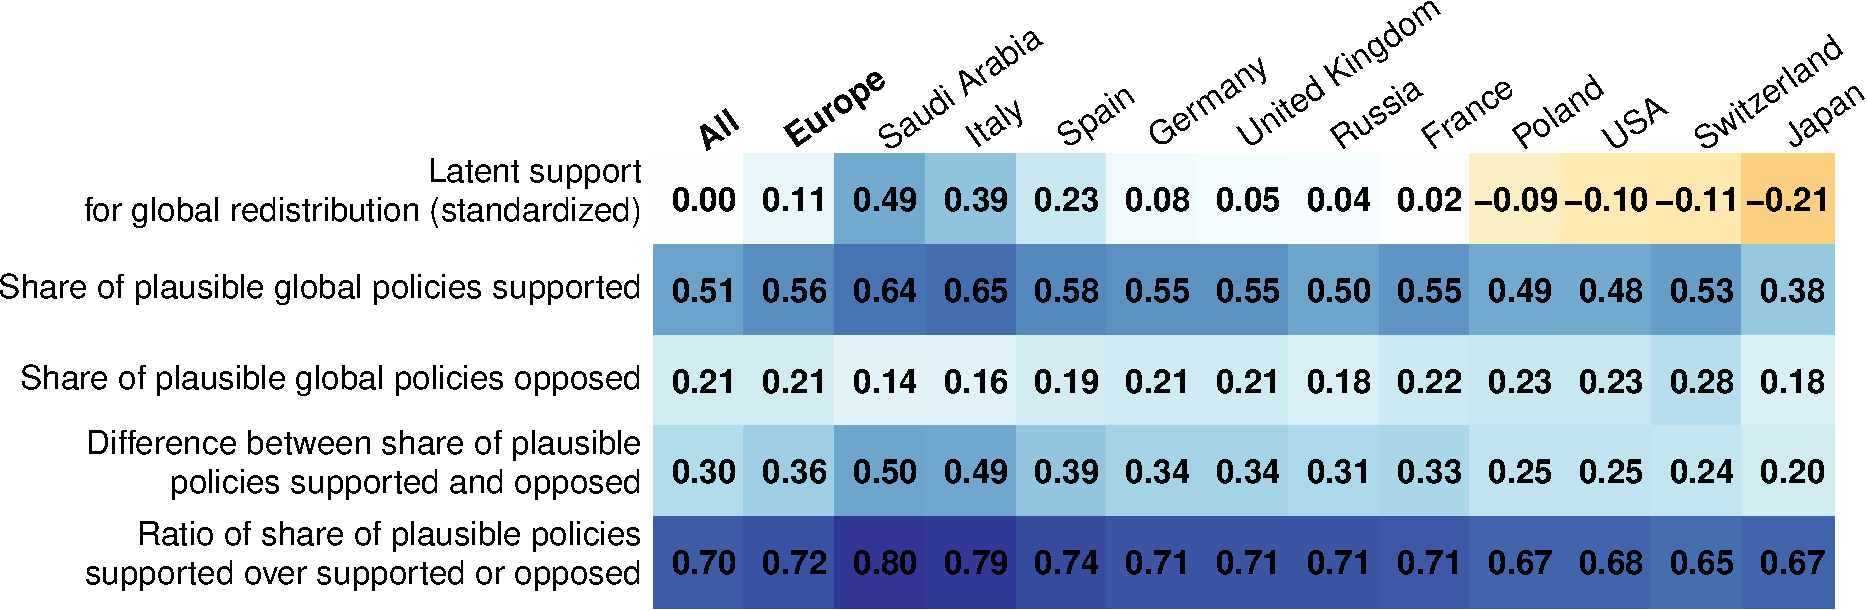
\includegraphics[width=\textwidth]{../figures/country_comparison/synthetic_indicators_mean.pdf}} 
\end{figure}

\begin{figure}[h!]
    \caption[Willingness to participate in a global movement for sustainable development]{``If there was a worldwide movement in favor of a global program to tackle climate change, implement taxes on millionaires and fund poverty reduction in low-income countries, to what extent would you be willing to be part of that movement? (Multiple answers possible)'' (Question~\ref{q:global_movement}). \hfill (Back~to~Section~\ref{par:willingness_act}.)
    }\label{fig:global_movement}
    \makebox[\textwidth][c]{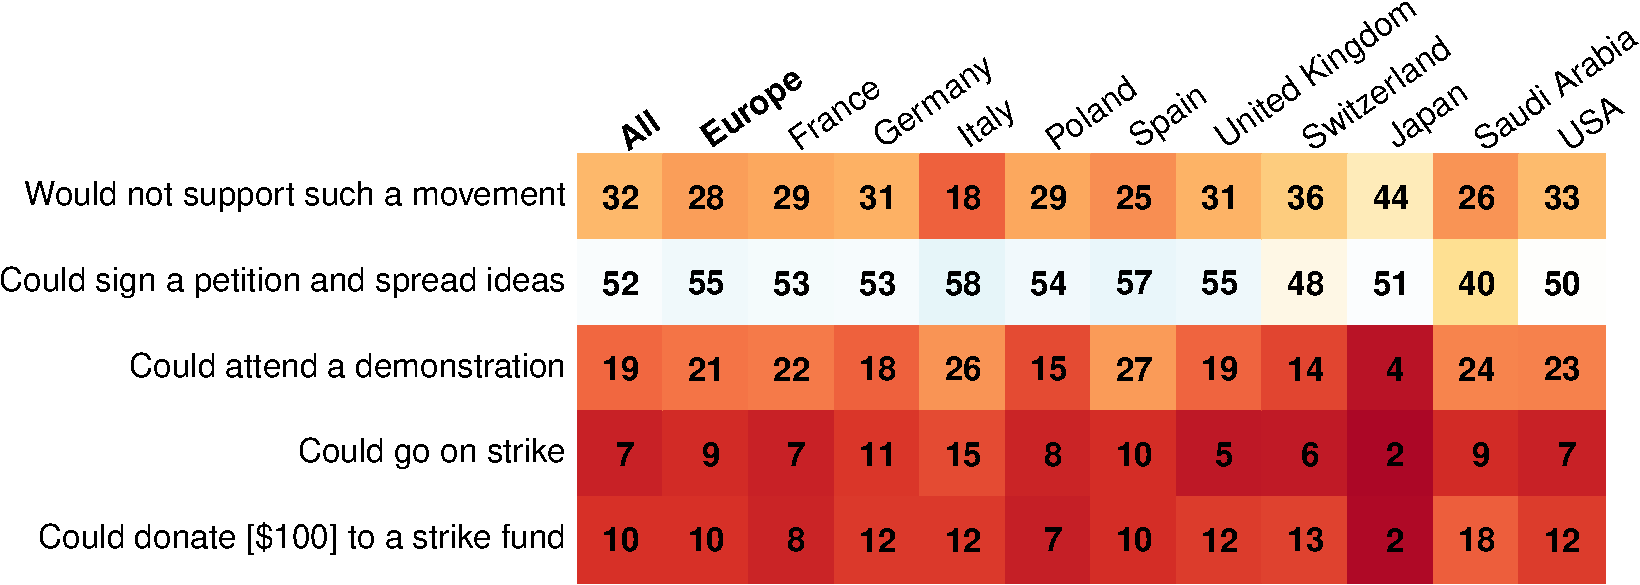
\includegraphics[width=\textwidth]{../figures/country_comparison/global_movement_positive.pdf}} 
\end{figure}

% \begin{figure}[h!]
%     \caption[Keyword classification of open-ended fields]{Keyword classification of open-ended fields (matches with at least one keyword in a list). (Questions~\ref{q:concerns_field}-\ref{q:injustice_field}). \hfill (Back~to~Section~\ref{subsec:considerations}.)
%     }\label{fig:field_keyword}
%     \makebox[\textwidth][c]{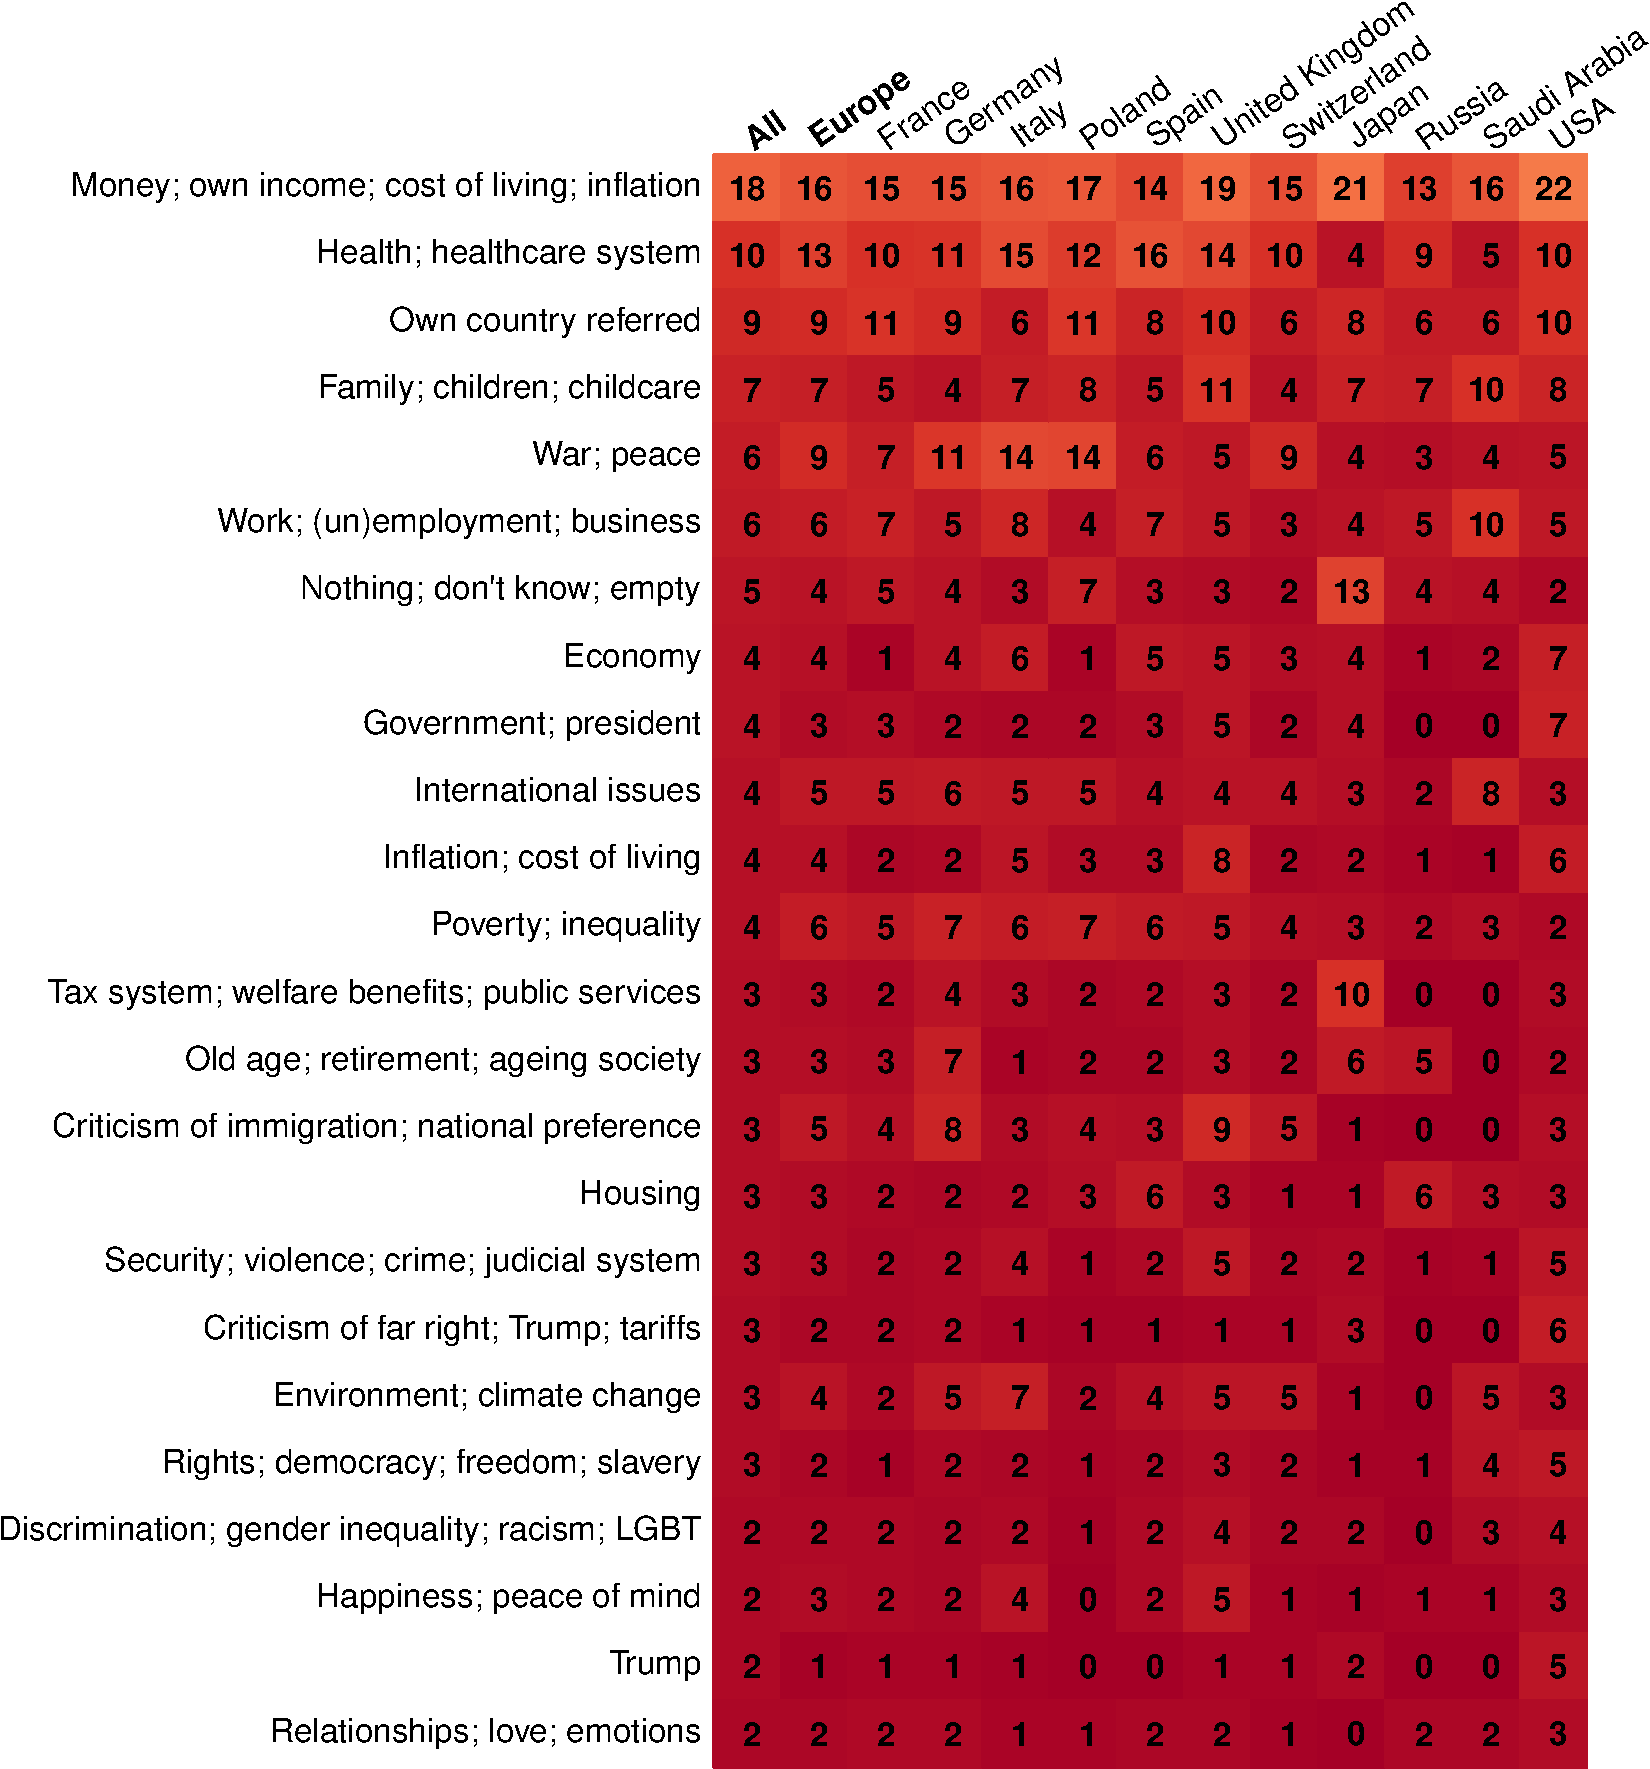
\includegraphics[height=.85\textheight]{../figures/country_comparison/field_keyword_main_positive.pdf}} 
% \end{figure}

% \begin{figure}[h!]
%     \caption[AI classification of open-ended fields]{AI classification of open-ended fields (using ChatGPT-4.1). (Questions~\ref{q:concerns_field}-\ref{q:injustice_field}).\hfill (Back~to~Section~\ref{subsec:considerations}.)
%     }\label{fig:field_gpt}
%     \makebox[\textwidth][c]{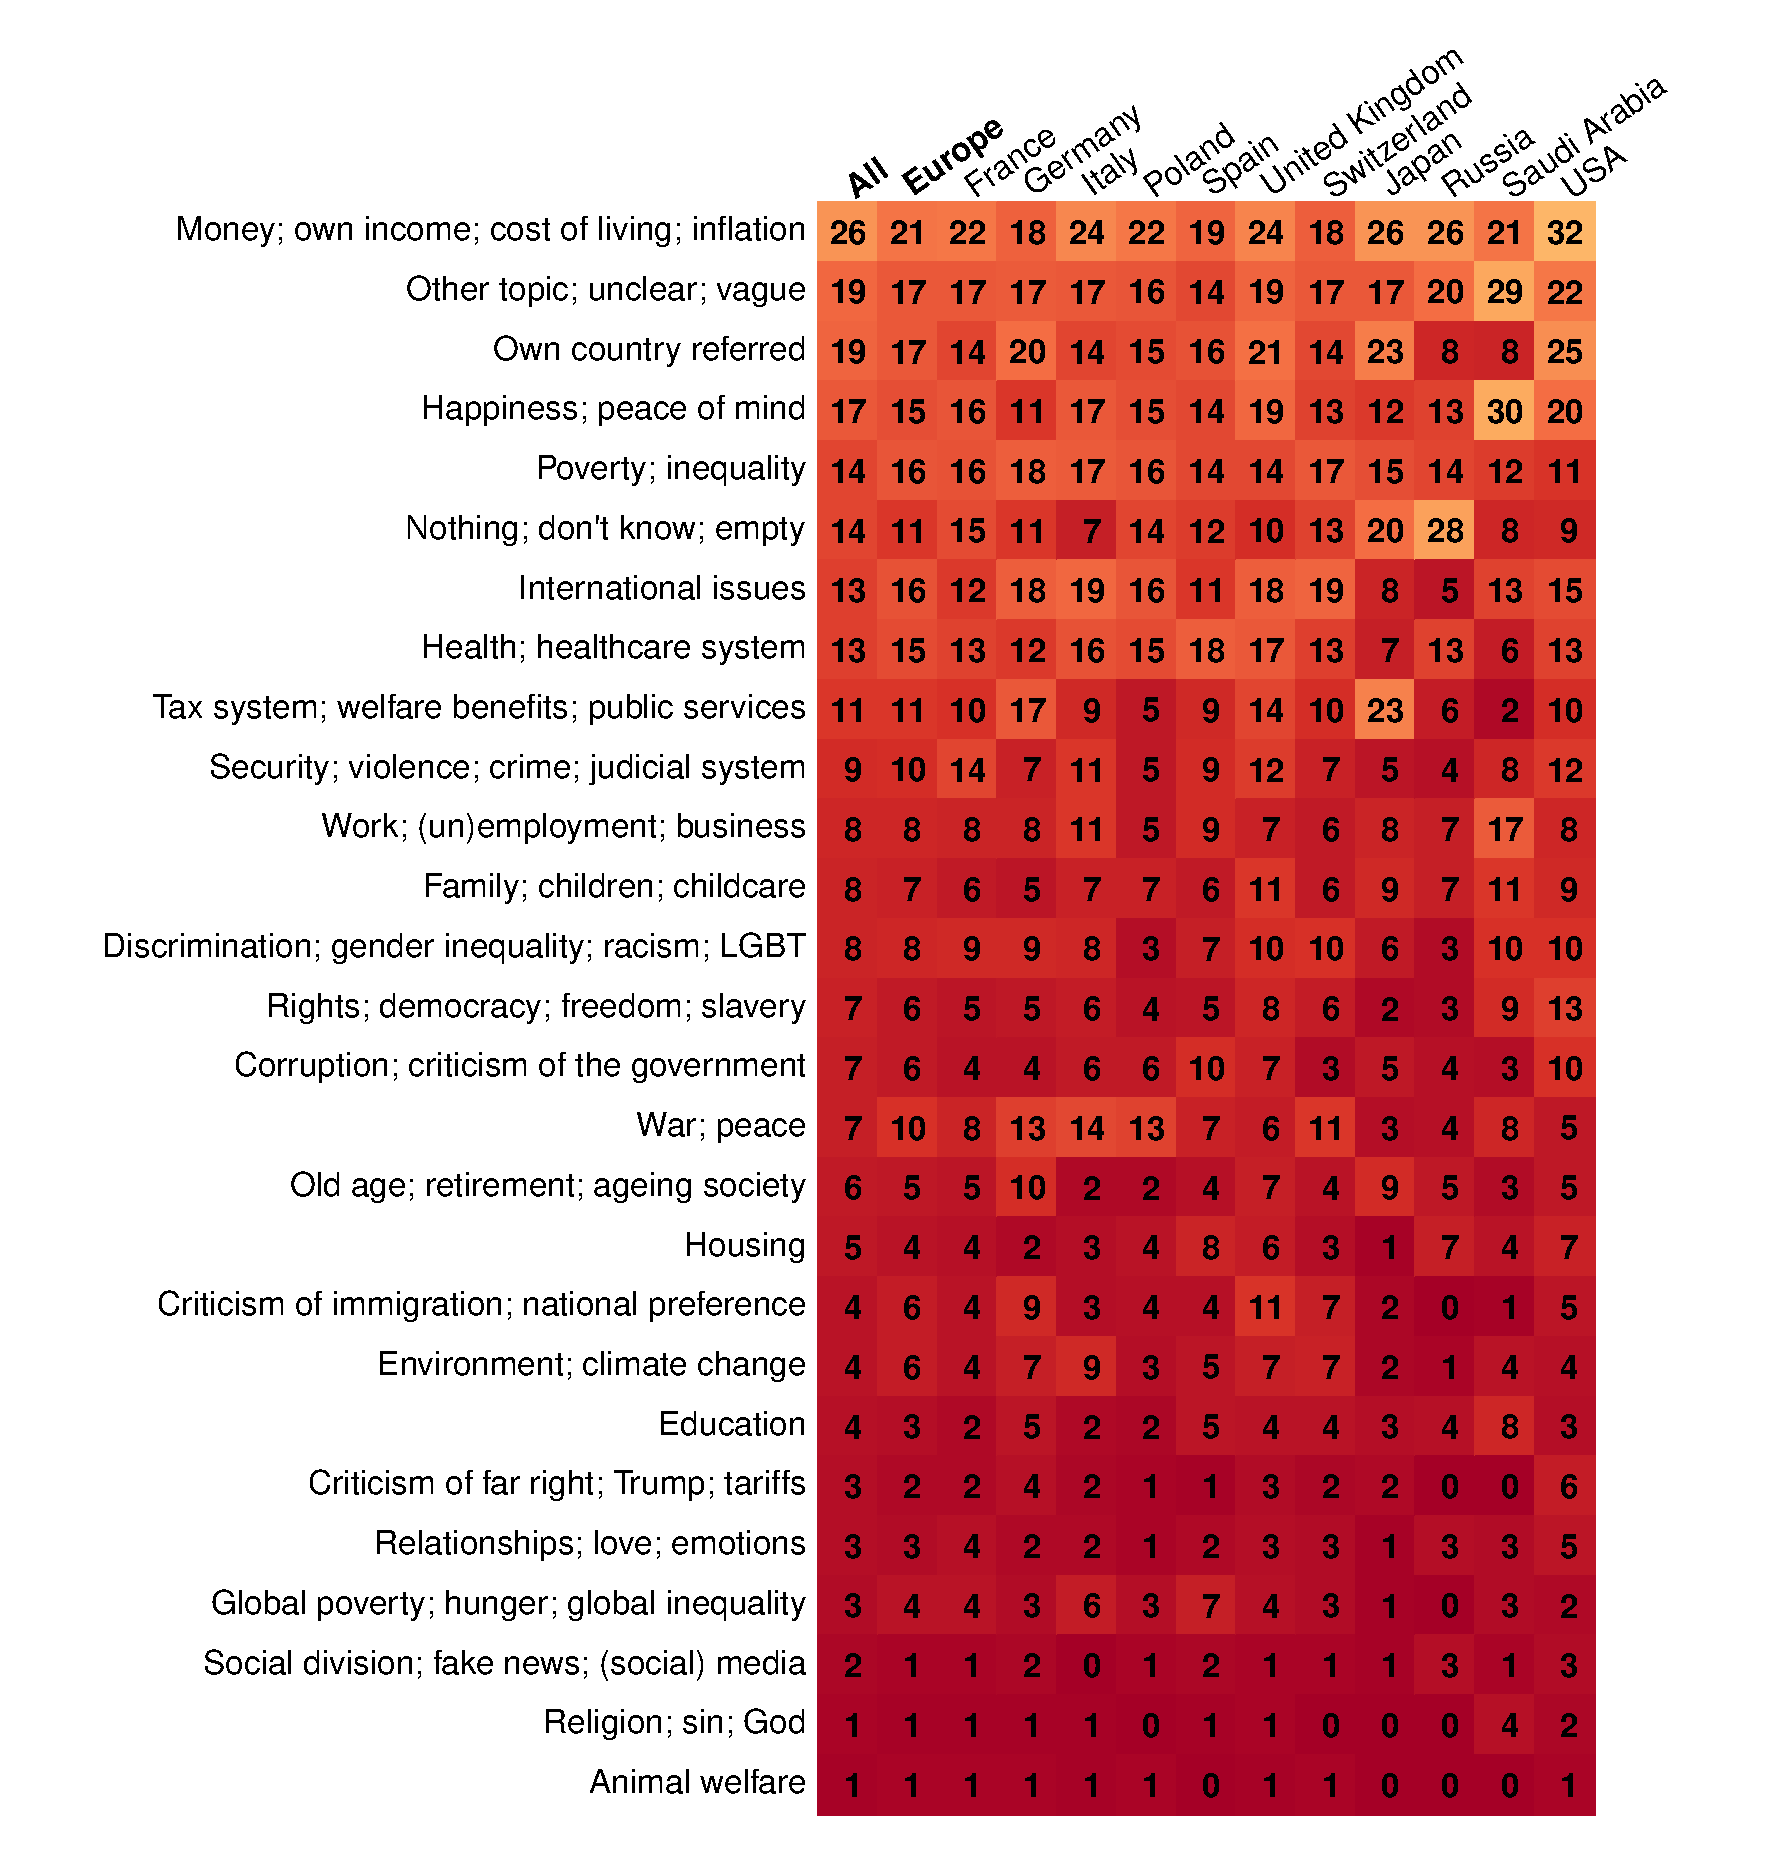
\includegraphics[height=.85\textheight]{../figures/country_comparison/field_gpt_positive.pdf}} 
% \end{figure}

\begin{figure}[h!]
    \caption[Manual classification of open-ended fields]{Manual classification of open-ended fields. (Questions~\ref{q:concerns_field}-\ref{q:injustice_field}).\hfill (Back~to~Section~\ref{subsec:considerations}.)
    }\label{fig:field_manual}
    \makebox[\textwidth][c]{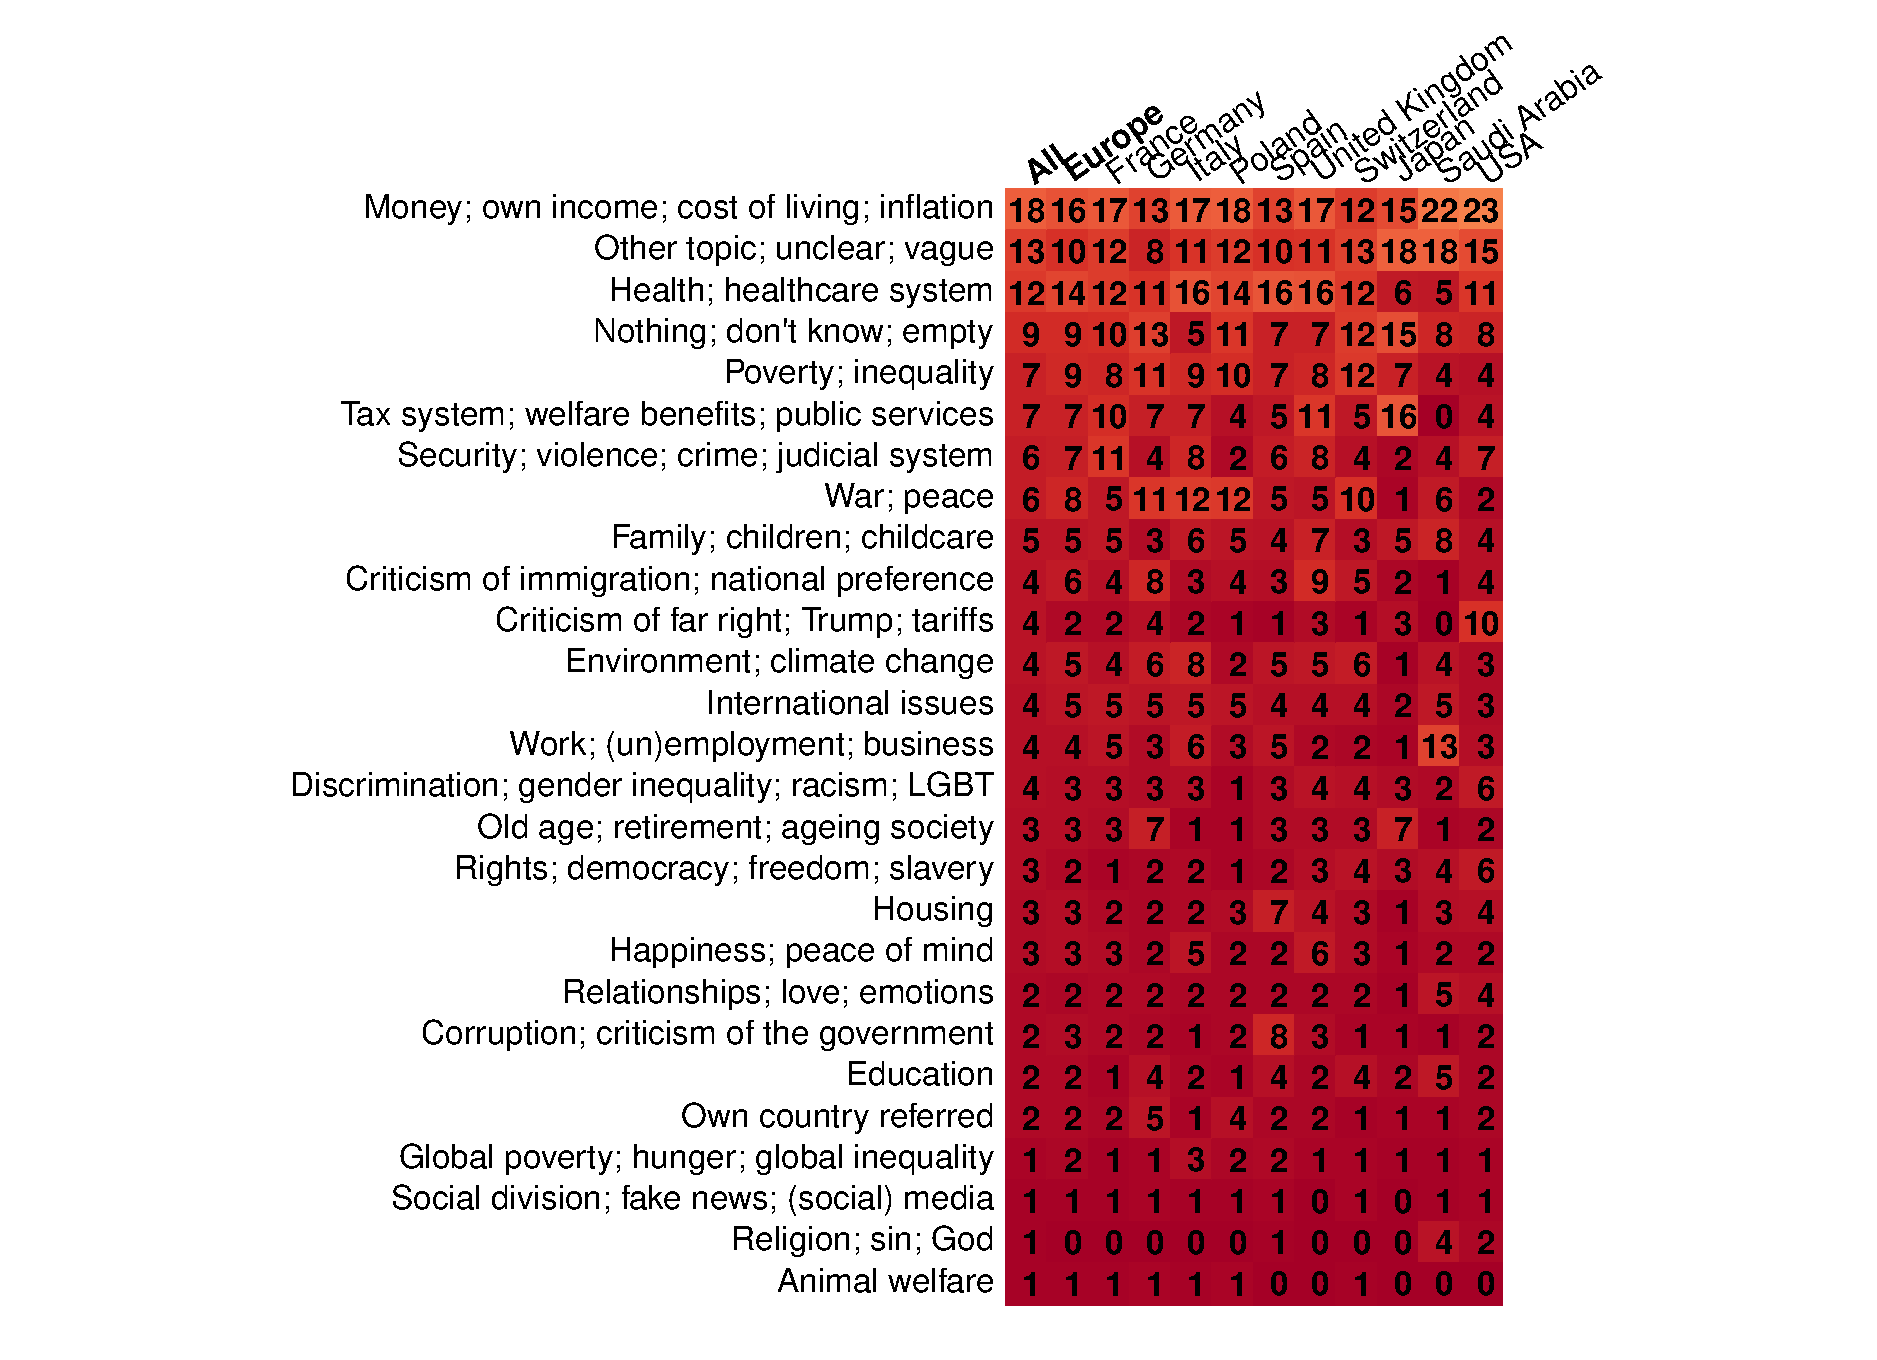
\includegraphics[height=.85\textheight]{../figures/country_comparison/field_manual_positive.pdf}} 
\end{figure}

\begin{figure}[h!]
    \caption[Manual classification of \textit{concerns} fields]{Manual classification of \textit{concerns} fields: ``What are your main concerns these days?'' (Question~\ref{q:concerns_field}).\hfill (Back~to~Section~\ref{subsec:considerations}.)
    }\label{fig:concerns_field}
    \makebox[\textwidth][c]{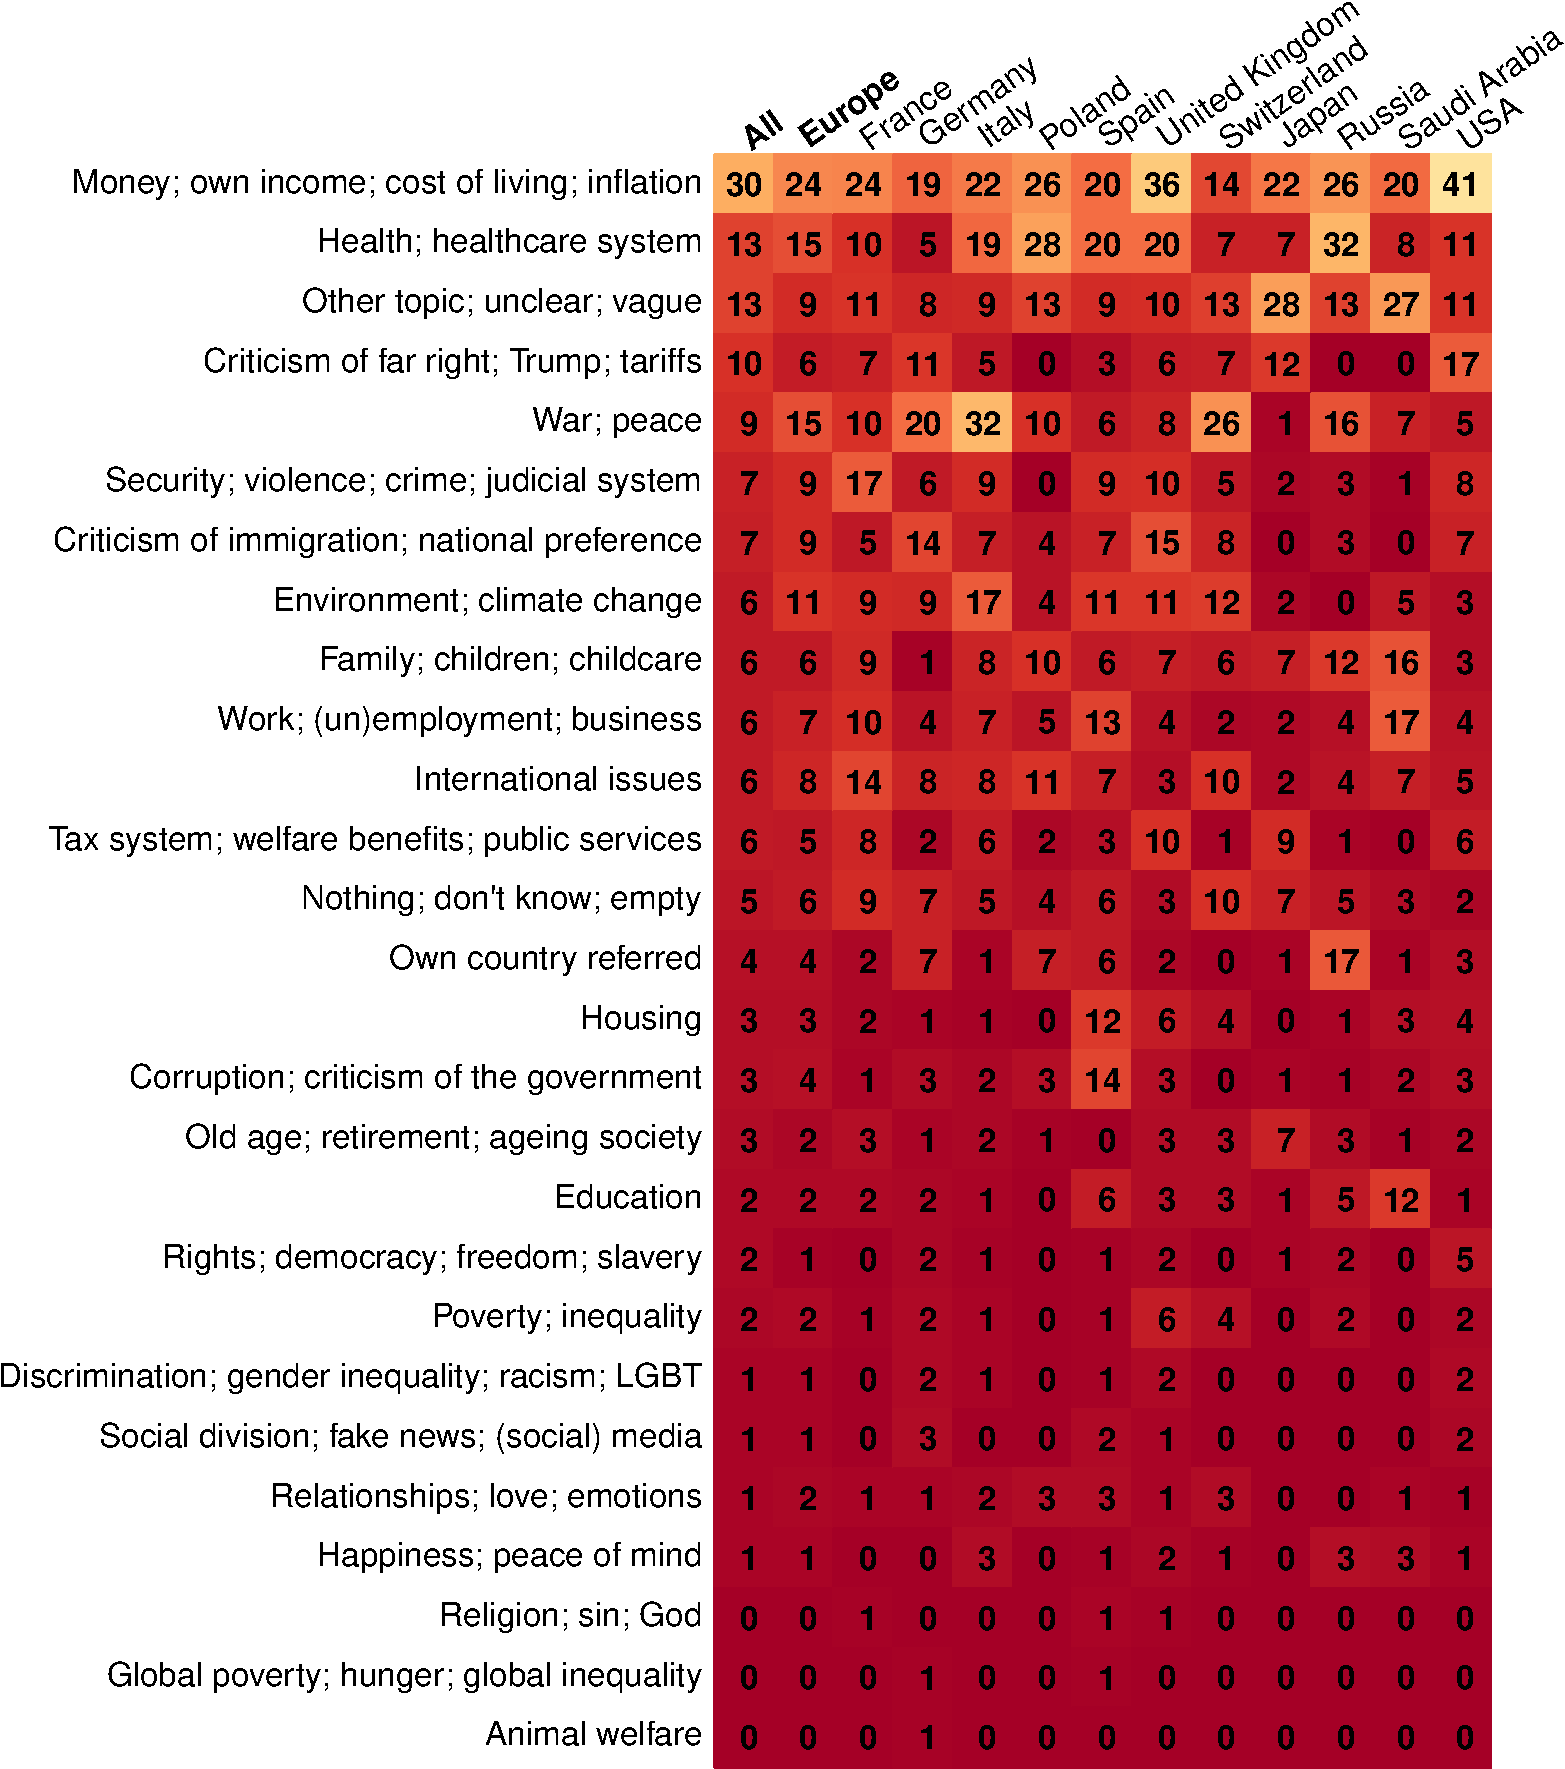
\includegraphics[height=.85\textheight]{../figures/country_comparison/field_concerns_manual_positive.pdf}} 
\end{figure}

\begin{figure}[h!]
    \caption[Manual classification of \textit{wish} fields]{Manual classification of \textit{wish} fields: ``What are your needs or wishes?'' (Question~\ref{q:wish_field}).\hfill (Back~to~Section~\ref{subsec:considerations}.)
    }\label{fig:wish_field}
    \makebox[\textwidth][c]{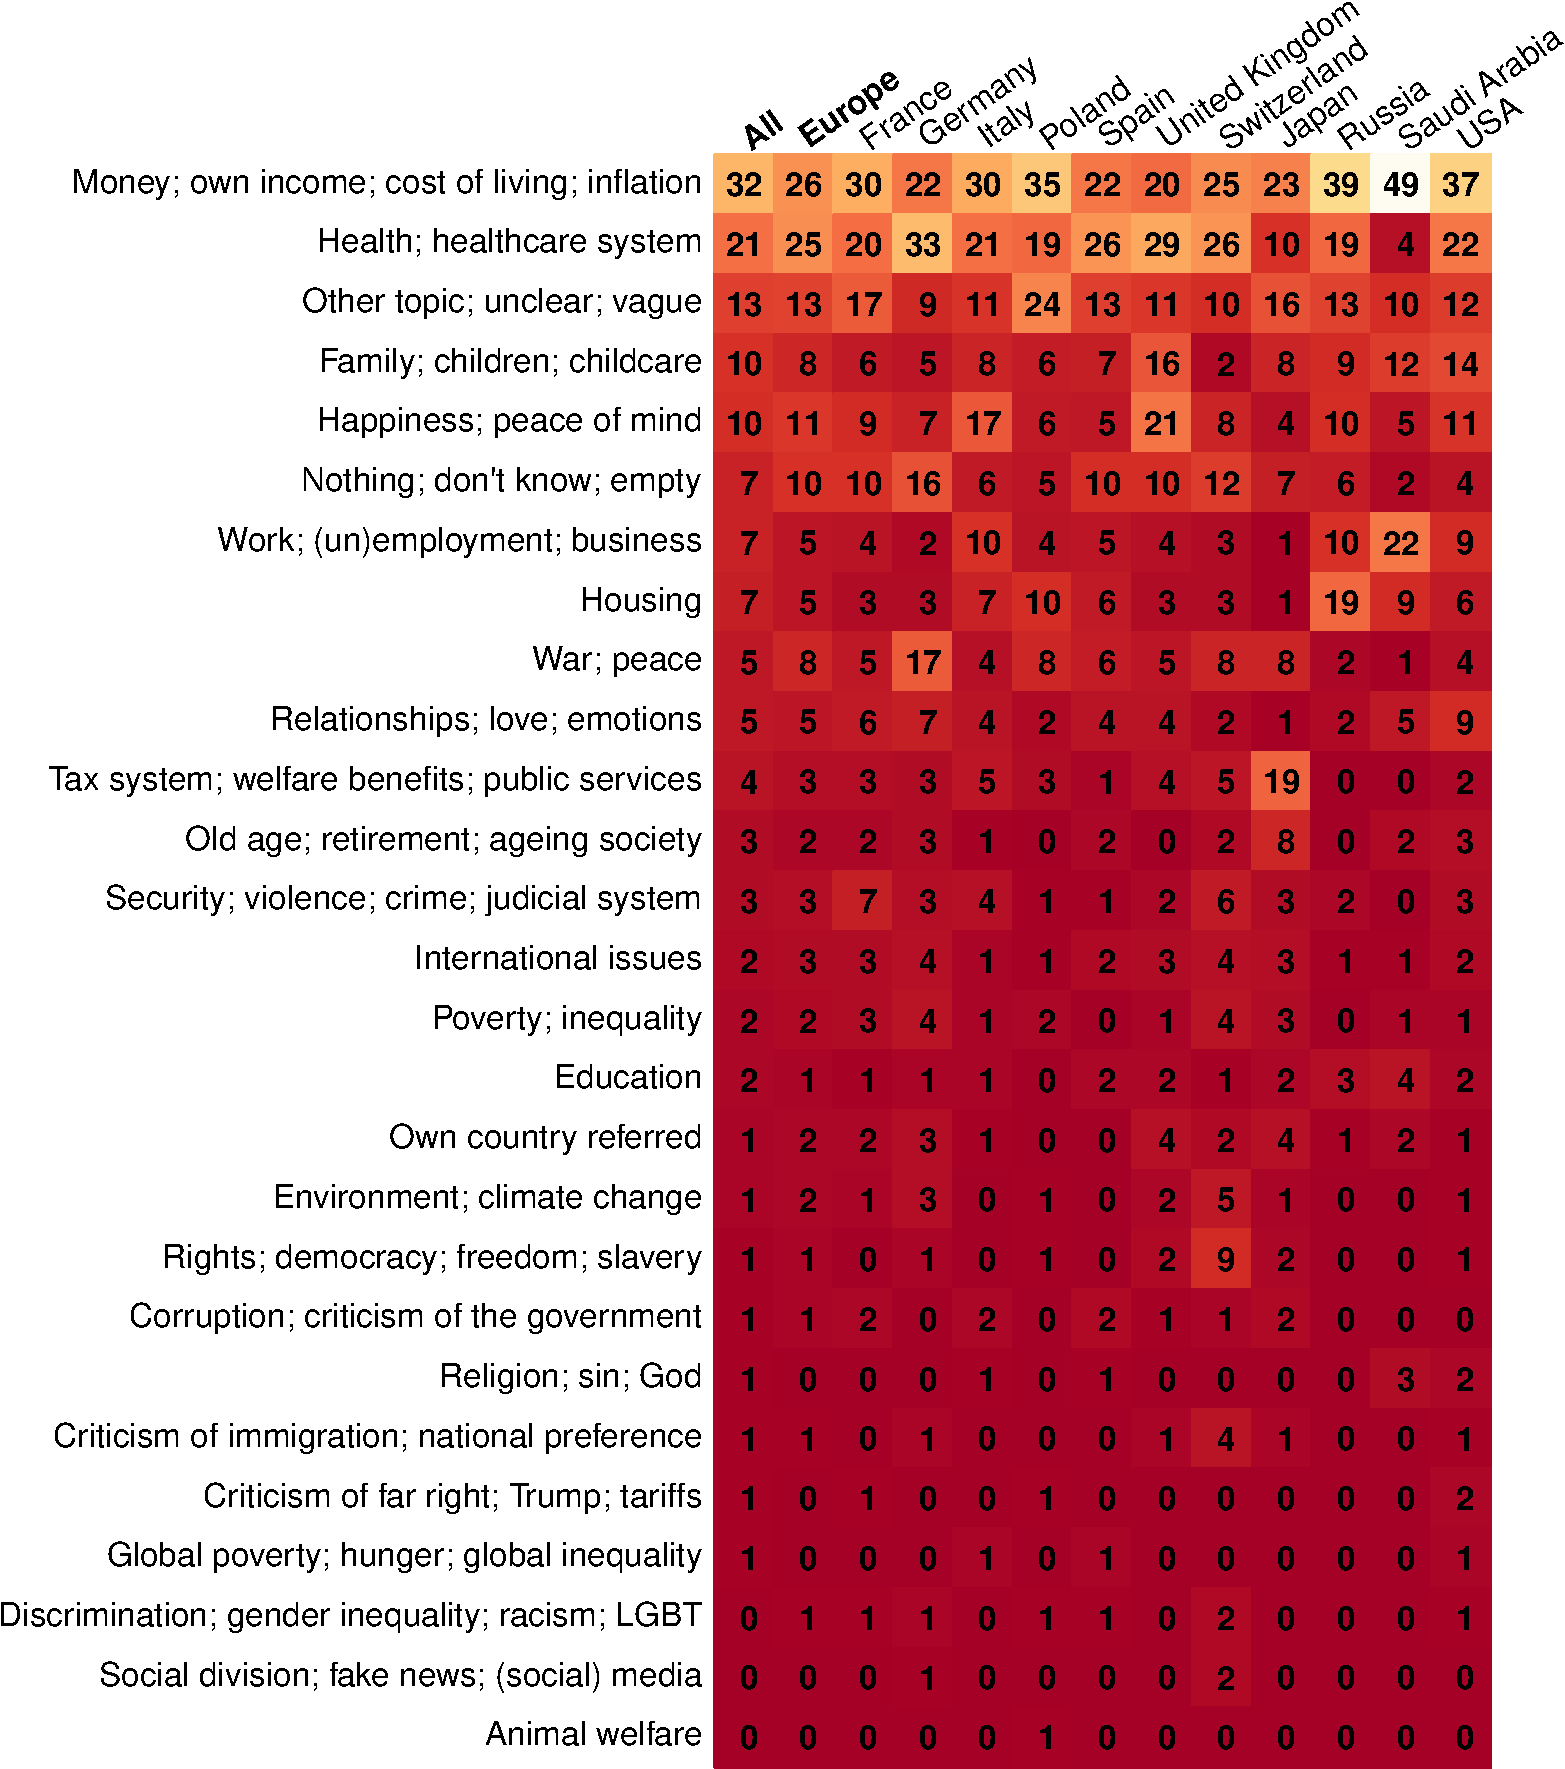
\includegraphics[height=.85\textheight]{../figures/country_comparison/field_wish_manual_positive.pdf}} 
\end{figure}

\begin{figure}[h!]
    \caption[Manual classification of \textit{injustice} fields]{Manual classification of \textit{injustice} fields: ``What according to you is the greatest injustice of all?'' (Question~\ref{q:injustice_field}).\hfill (Back~to~Section~\ref{subsec:considerations}.)
    }\label{fig:injustice_field}
    \makebox[\textwidth][c]{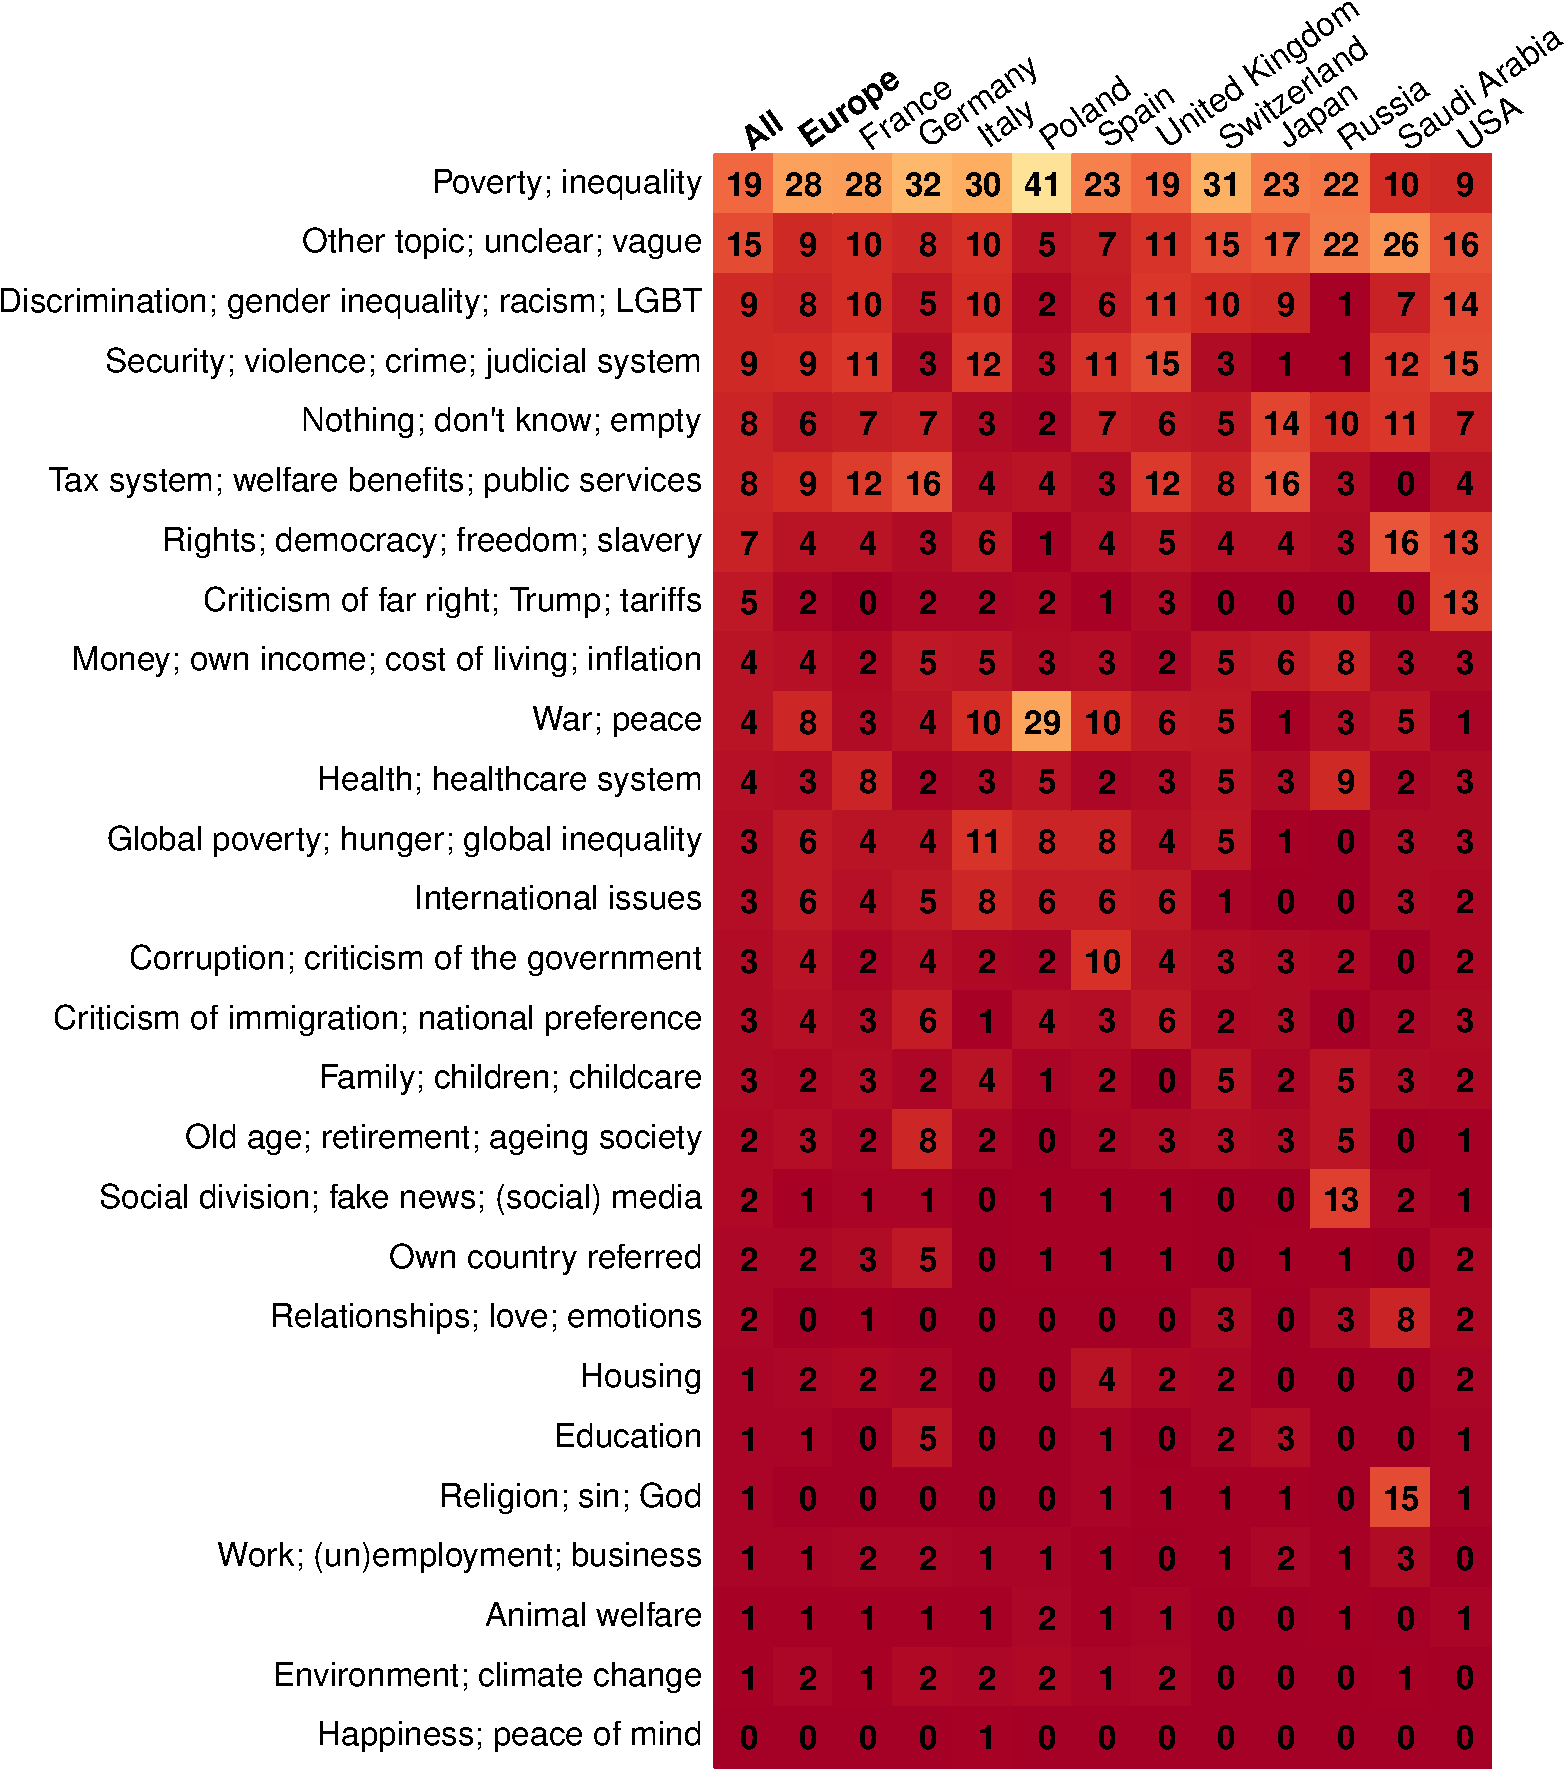
\includegraphics[height=.85\textheight]{../figures/country_comparison/field_injustice_manual_positive.pdf}} 
\end{figure}

\begin{figure}[h!]
    \caption[Manual classification of \textit{issue} fields]{Manual classification of \textit{issue} fields: ``Can you name an issue that is important to you but is neglected in the public debate?'' (Question~\ref{q:issue_field}).\hfill (Back~to~Section~\ref{subsec:considerations}.)
    }\label{fig:issue_field}
    \makebox[\textwidth][c]{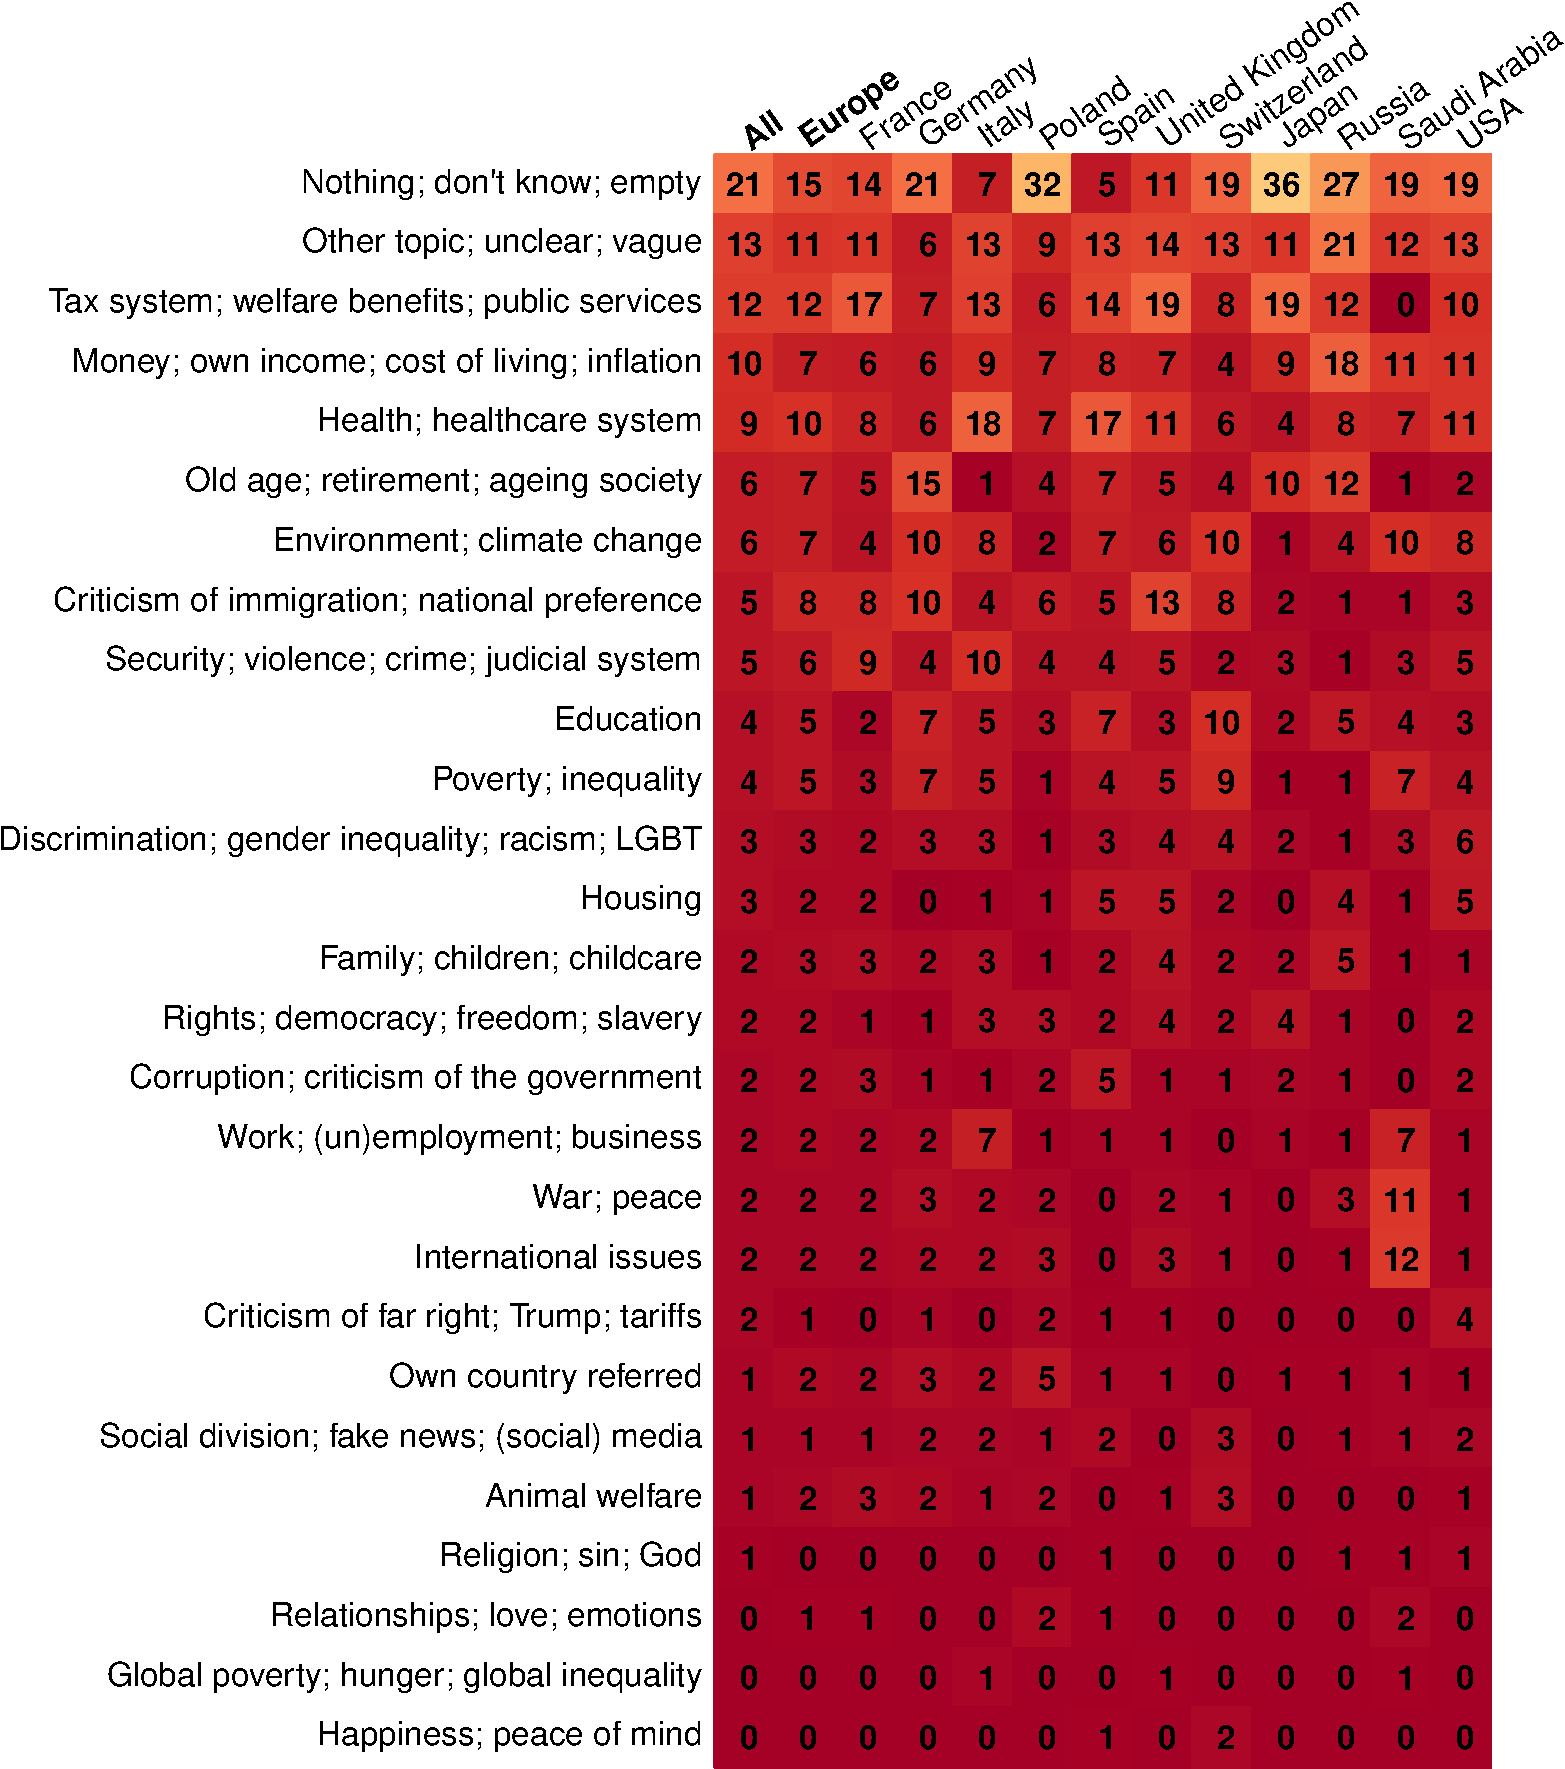
\includegraphics[height=.85\textheight]{../figures/country_comparison/field_issue_manual_positive.pdf}} 
\end{figure}

% \begin{figure}
% \caption[Conjoint analysis: effect of development aid and millionaire tax by vote]{Effect by vote at the last election on the likelihood that a political program is preferred of containing the following policy (compared to no foreign policy in the program). (See Figure \ref{fig:conjoint} for the simple figure). (Question~\ref{q:conjoint}). \hfill (Back~to~Section~\ref{subsec:considerations}.)} \label{fig:conjoint_vote}
% \begin{subfigure}{\textwidth}
%   \caption[]{Cut development aid.}
%   \makebox[\textwidth][c]{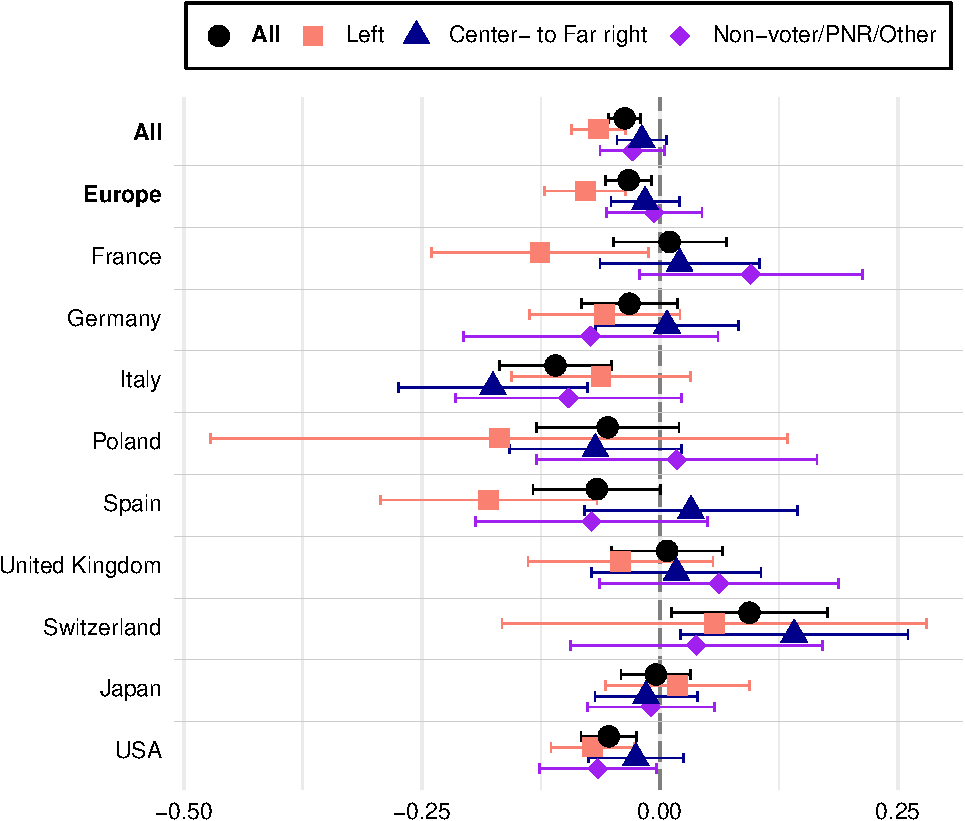
\includegraphics[width=.75\textwidth]{../figures/country_comparison/program_preferred_by_cut_aid_vote_country.pdf}}
% \end{subfigure} 
% \begin{subfigure}{\textwidth}
%   \caption[]{Int'l tax on millionaires with 30\% financing health and education in low-income countries.}%\begin{flushright}
%   \makebox[\textwidth][c]{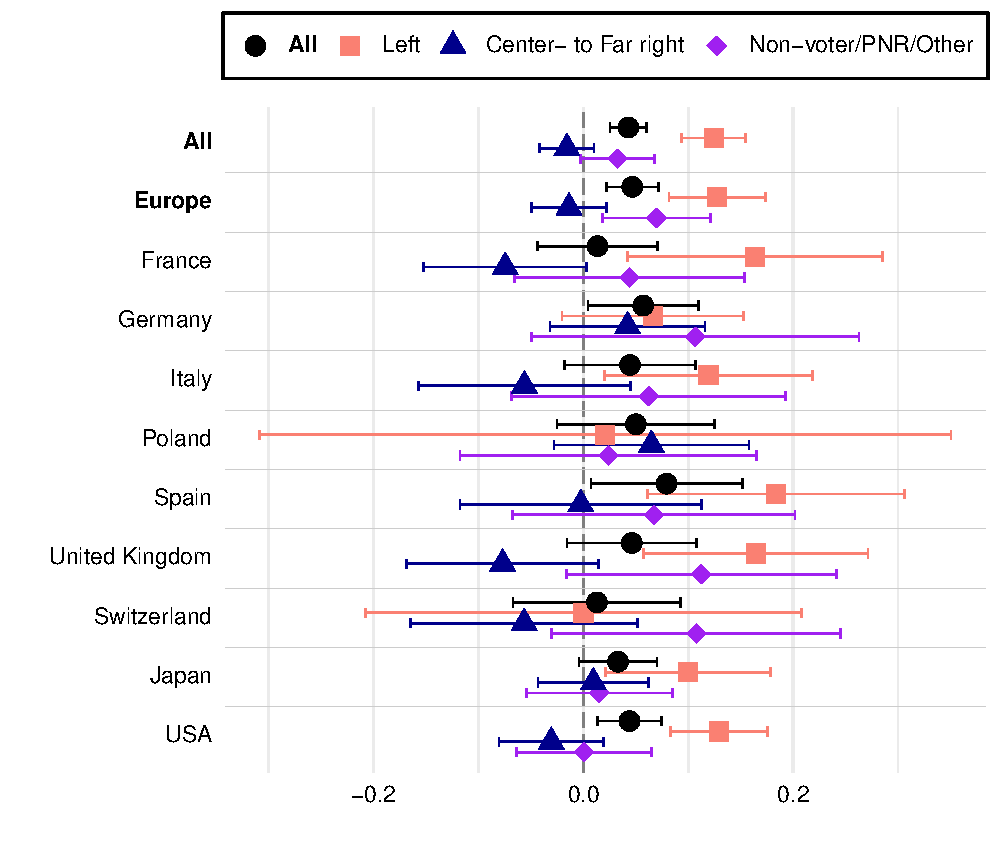
\includegraphics[width=.75\textwidth]{../figures/country_comparison/program_preferred_by_millionaire_tax_vote_country.pdf}}%\end{flushright}
% \end{subfigure}
% \end{figure}

% \begin{figure}[h!]
%     \caption[Conjoint analysis in France]{Conjoint analysis in France (Average Marginal Component Effect). Cf. Figure \ref{fig:conjoint_FR_original} for French. (Question~\ref{q:conjoint}). \hfill (Back~to~Section~\ref{subsec:conjoint}.)
%     }\label{fig:conjoint_FR}
%     \makebox[\textwidth][c]{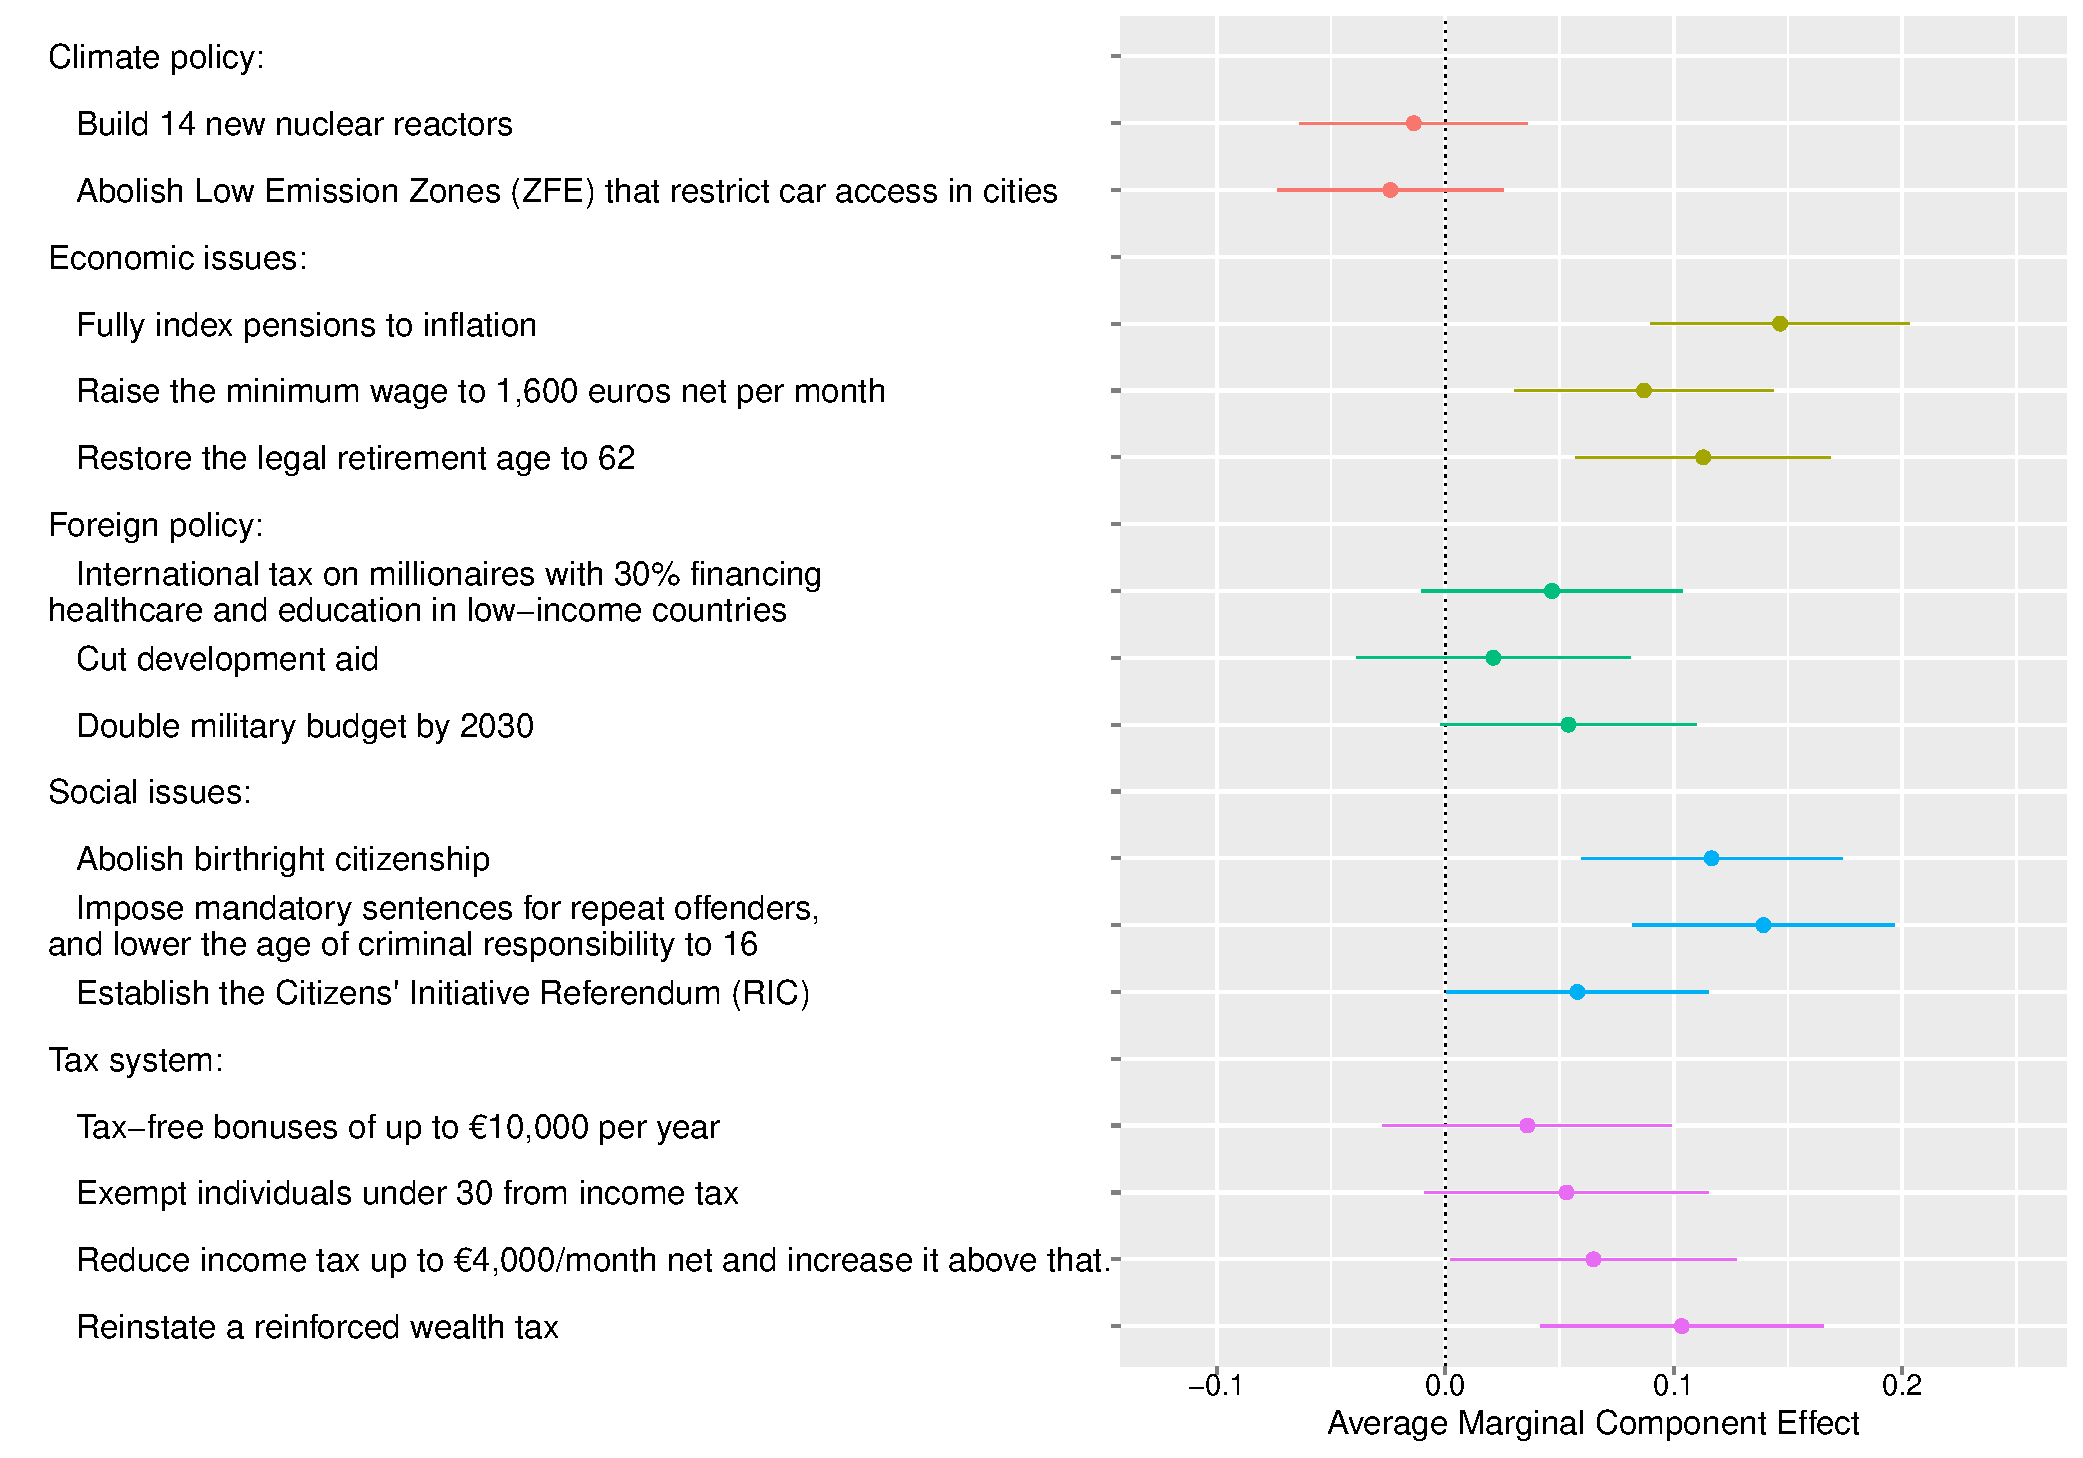
\includegraphics[width=\textwidth]{../figures/all/conjoint_EN-FR.pdf}} 
% \end{figure}

% \begin{figure}[h!]
%     \caption[Conjoint analysis in Germany]{Conjoint analysis in Germany (Average Marginal Component Effect). Cf. Figure \ref{fig:conjoint_DE_original} for German. (Question~\ref{q:conjoint}). \hfill (Back~to~Section~\ref{subsec:conjoint}.)
%     }\label{fig:conjoint_DE}
%     \makebox[\textwidth][c]{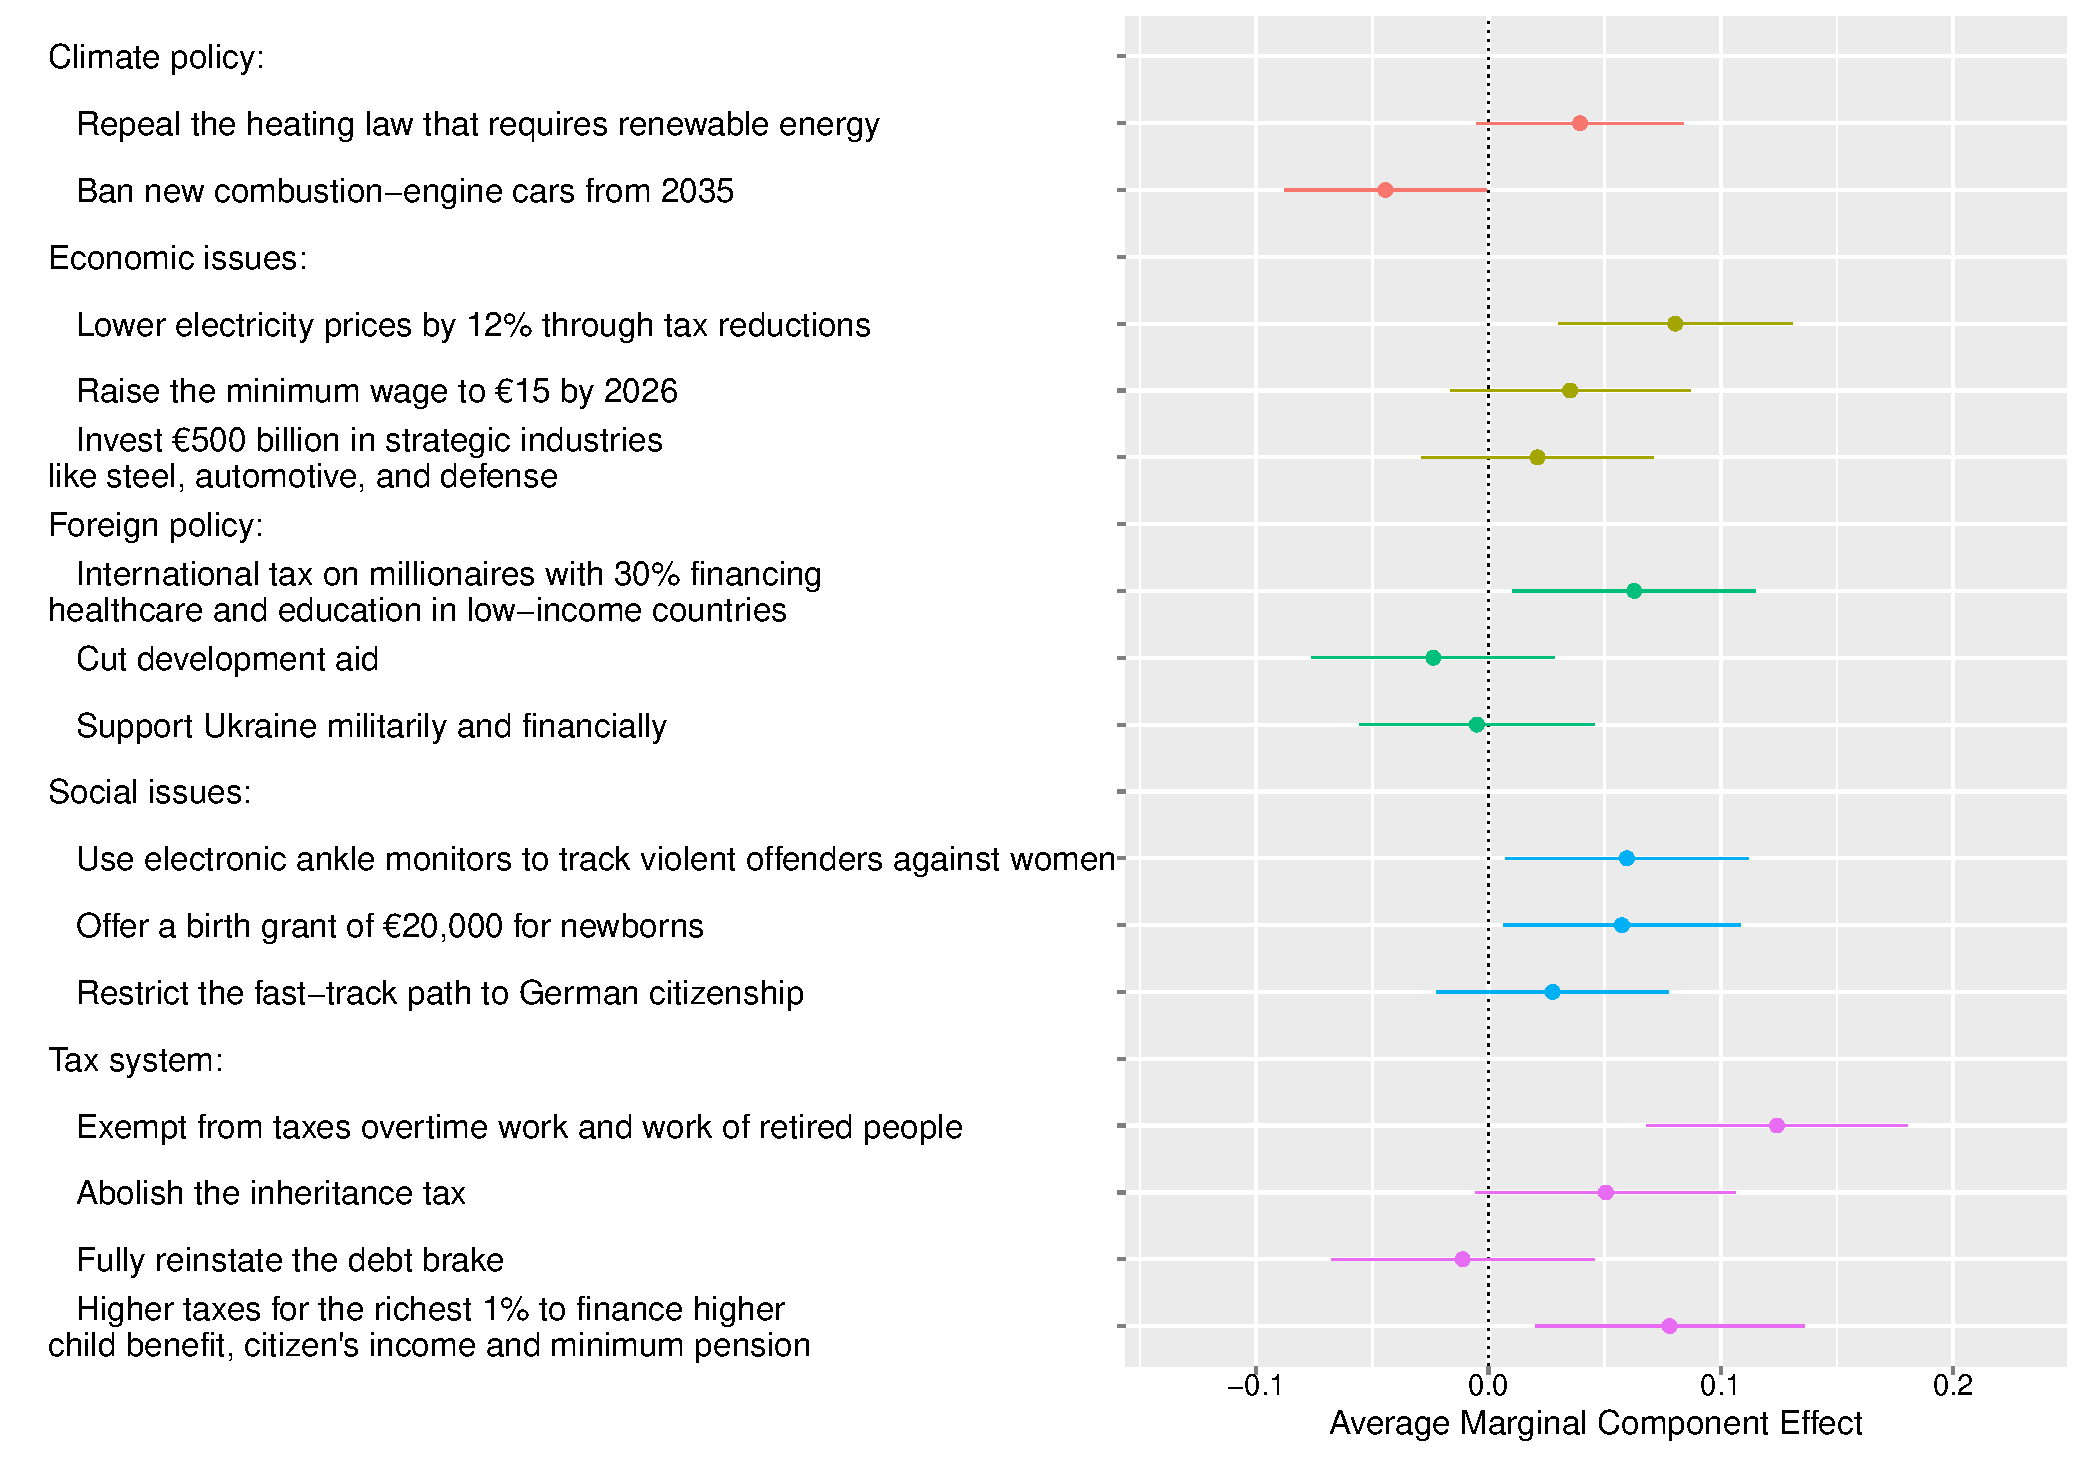
\includegraphics[width=\textwidth]{../figures/all/conjoint_EN-DE.pdf}} 
% \end{figure}

% \begin{figure}[h!]
%     \caption[Conjoint analysis in Italy]{Conjoint analysis in Italy (Average Marginal Component Effect). Cf. Figure \ref{fig:conjoint_IT_original} for Italian. (Question~\ref{q:conjoint}). \hfill (Back~to~Section~\ref{subsec:conjoint}.)
%     }\label{fig:conjoint_IT}
%     \makebox[\textwidth][c]{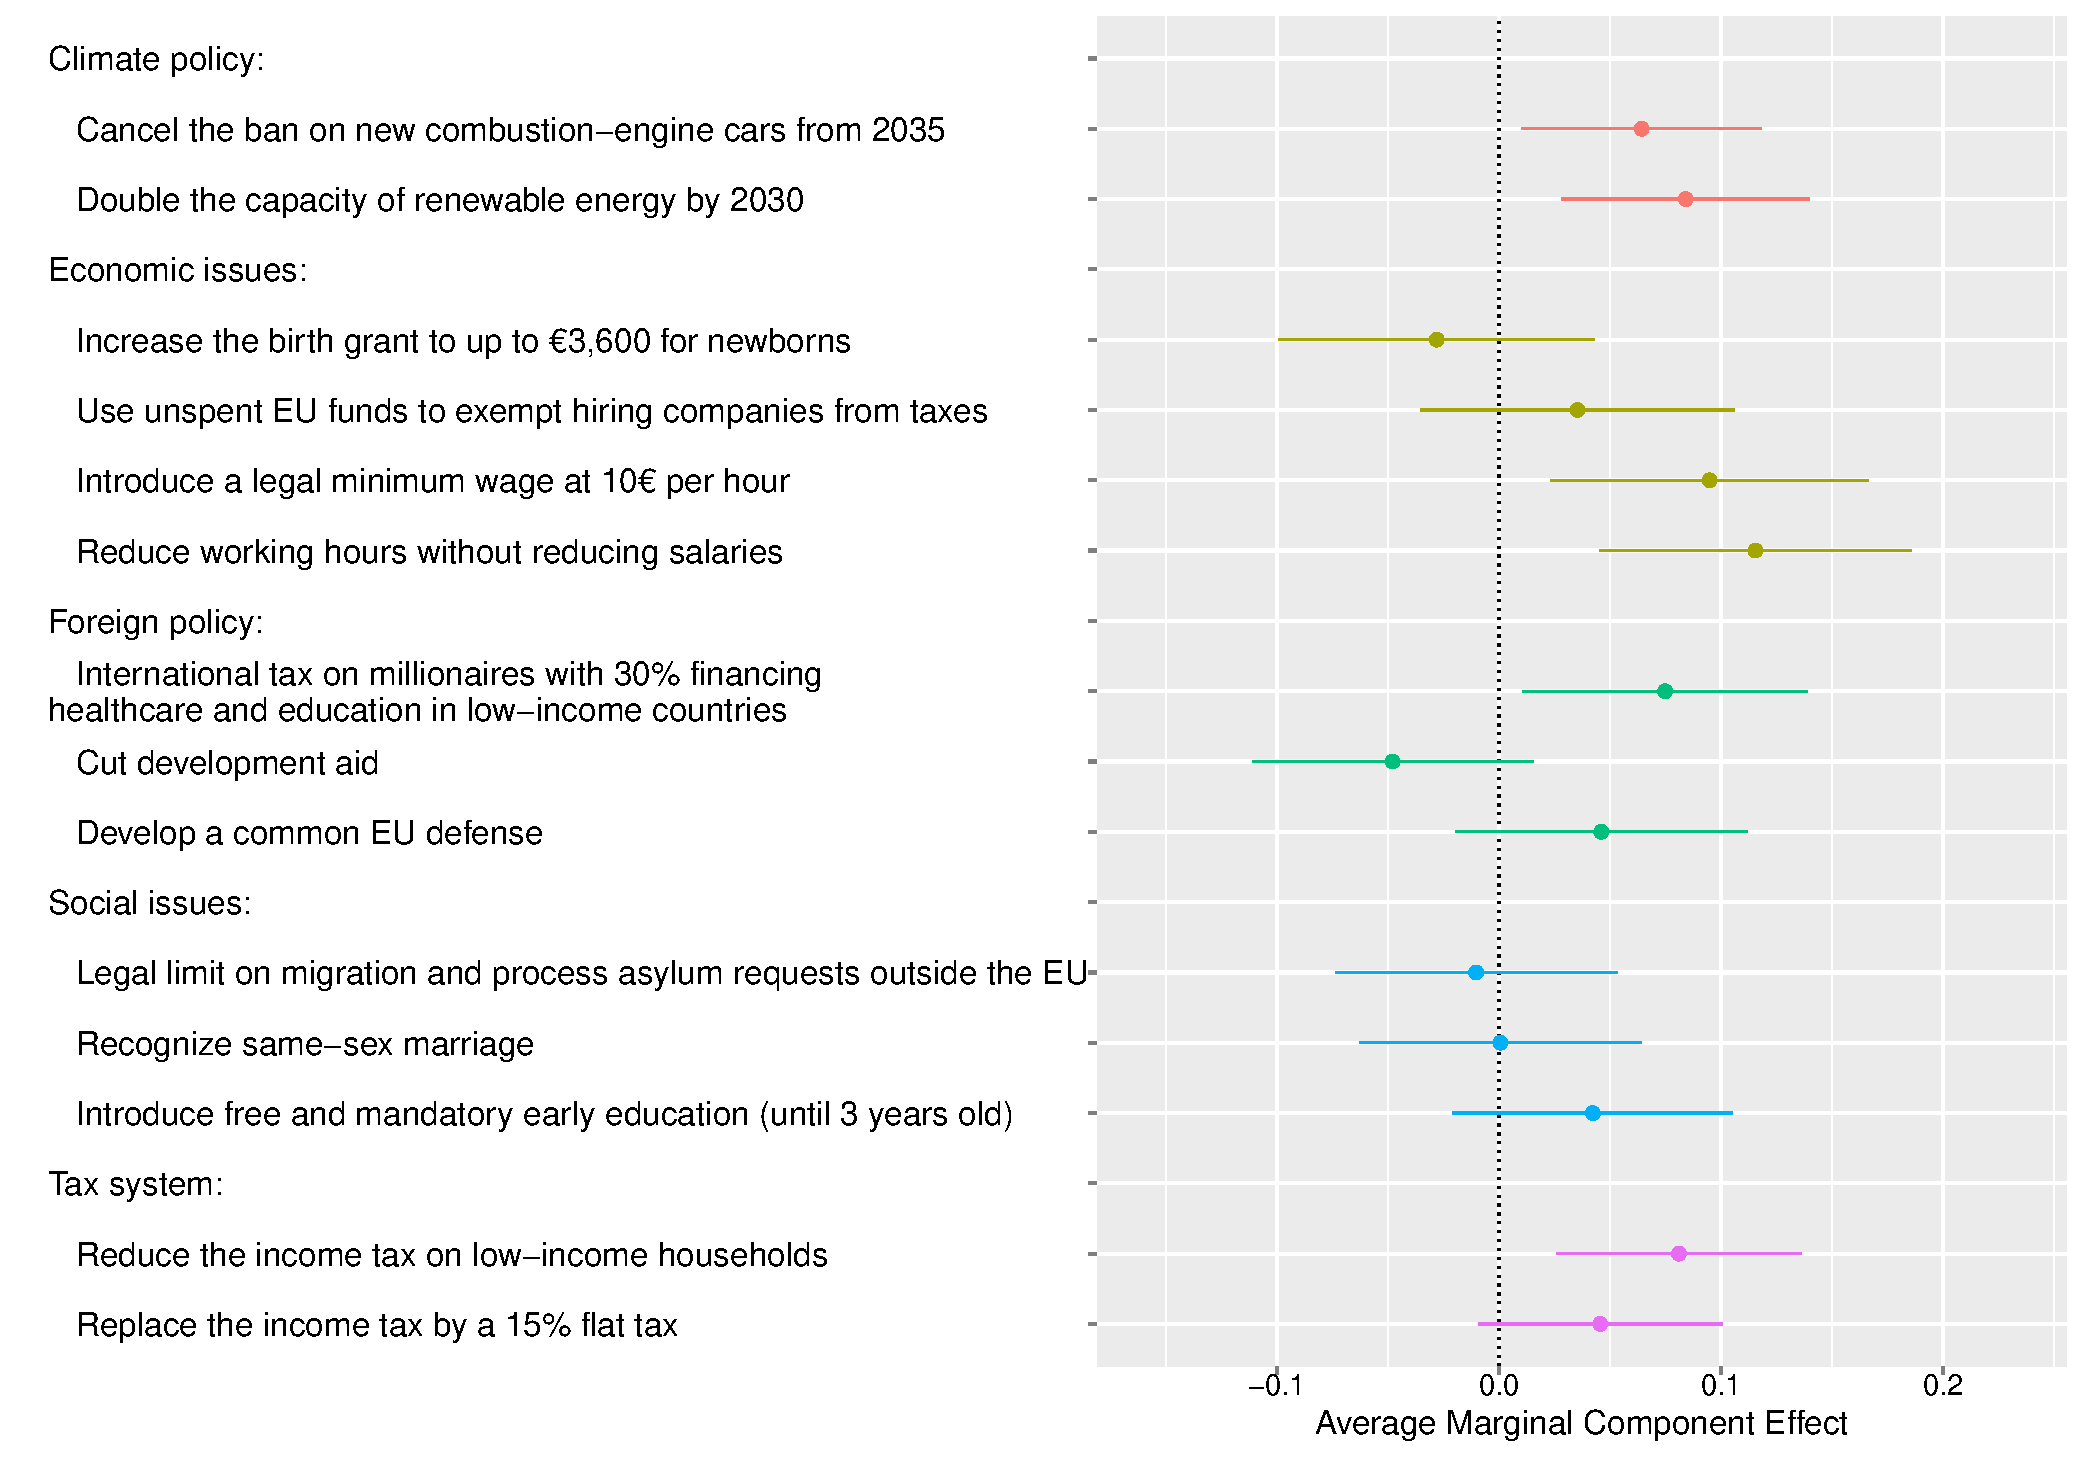
\includegraphics[width=\textwidth]{../figures/all/conjoint_EN-IT.pdf}} 
% \end{figure}

% \begin{figure}[h!]
%     \caption[Conjoint analysis in Poland]{Conjoint analysis in Poland (Average Marginal Component Effect). Cf. Figure \ref{fig:conjoint_PL_original} for Polish. (Question~\ref{q:conjoint}). \hfill (Back~to~Section~\ref{subsec:conjoint}.)
%     }\label{fig:conjoint_PL}
%     \makebox[\textwidth][c]{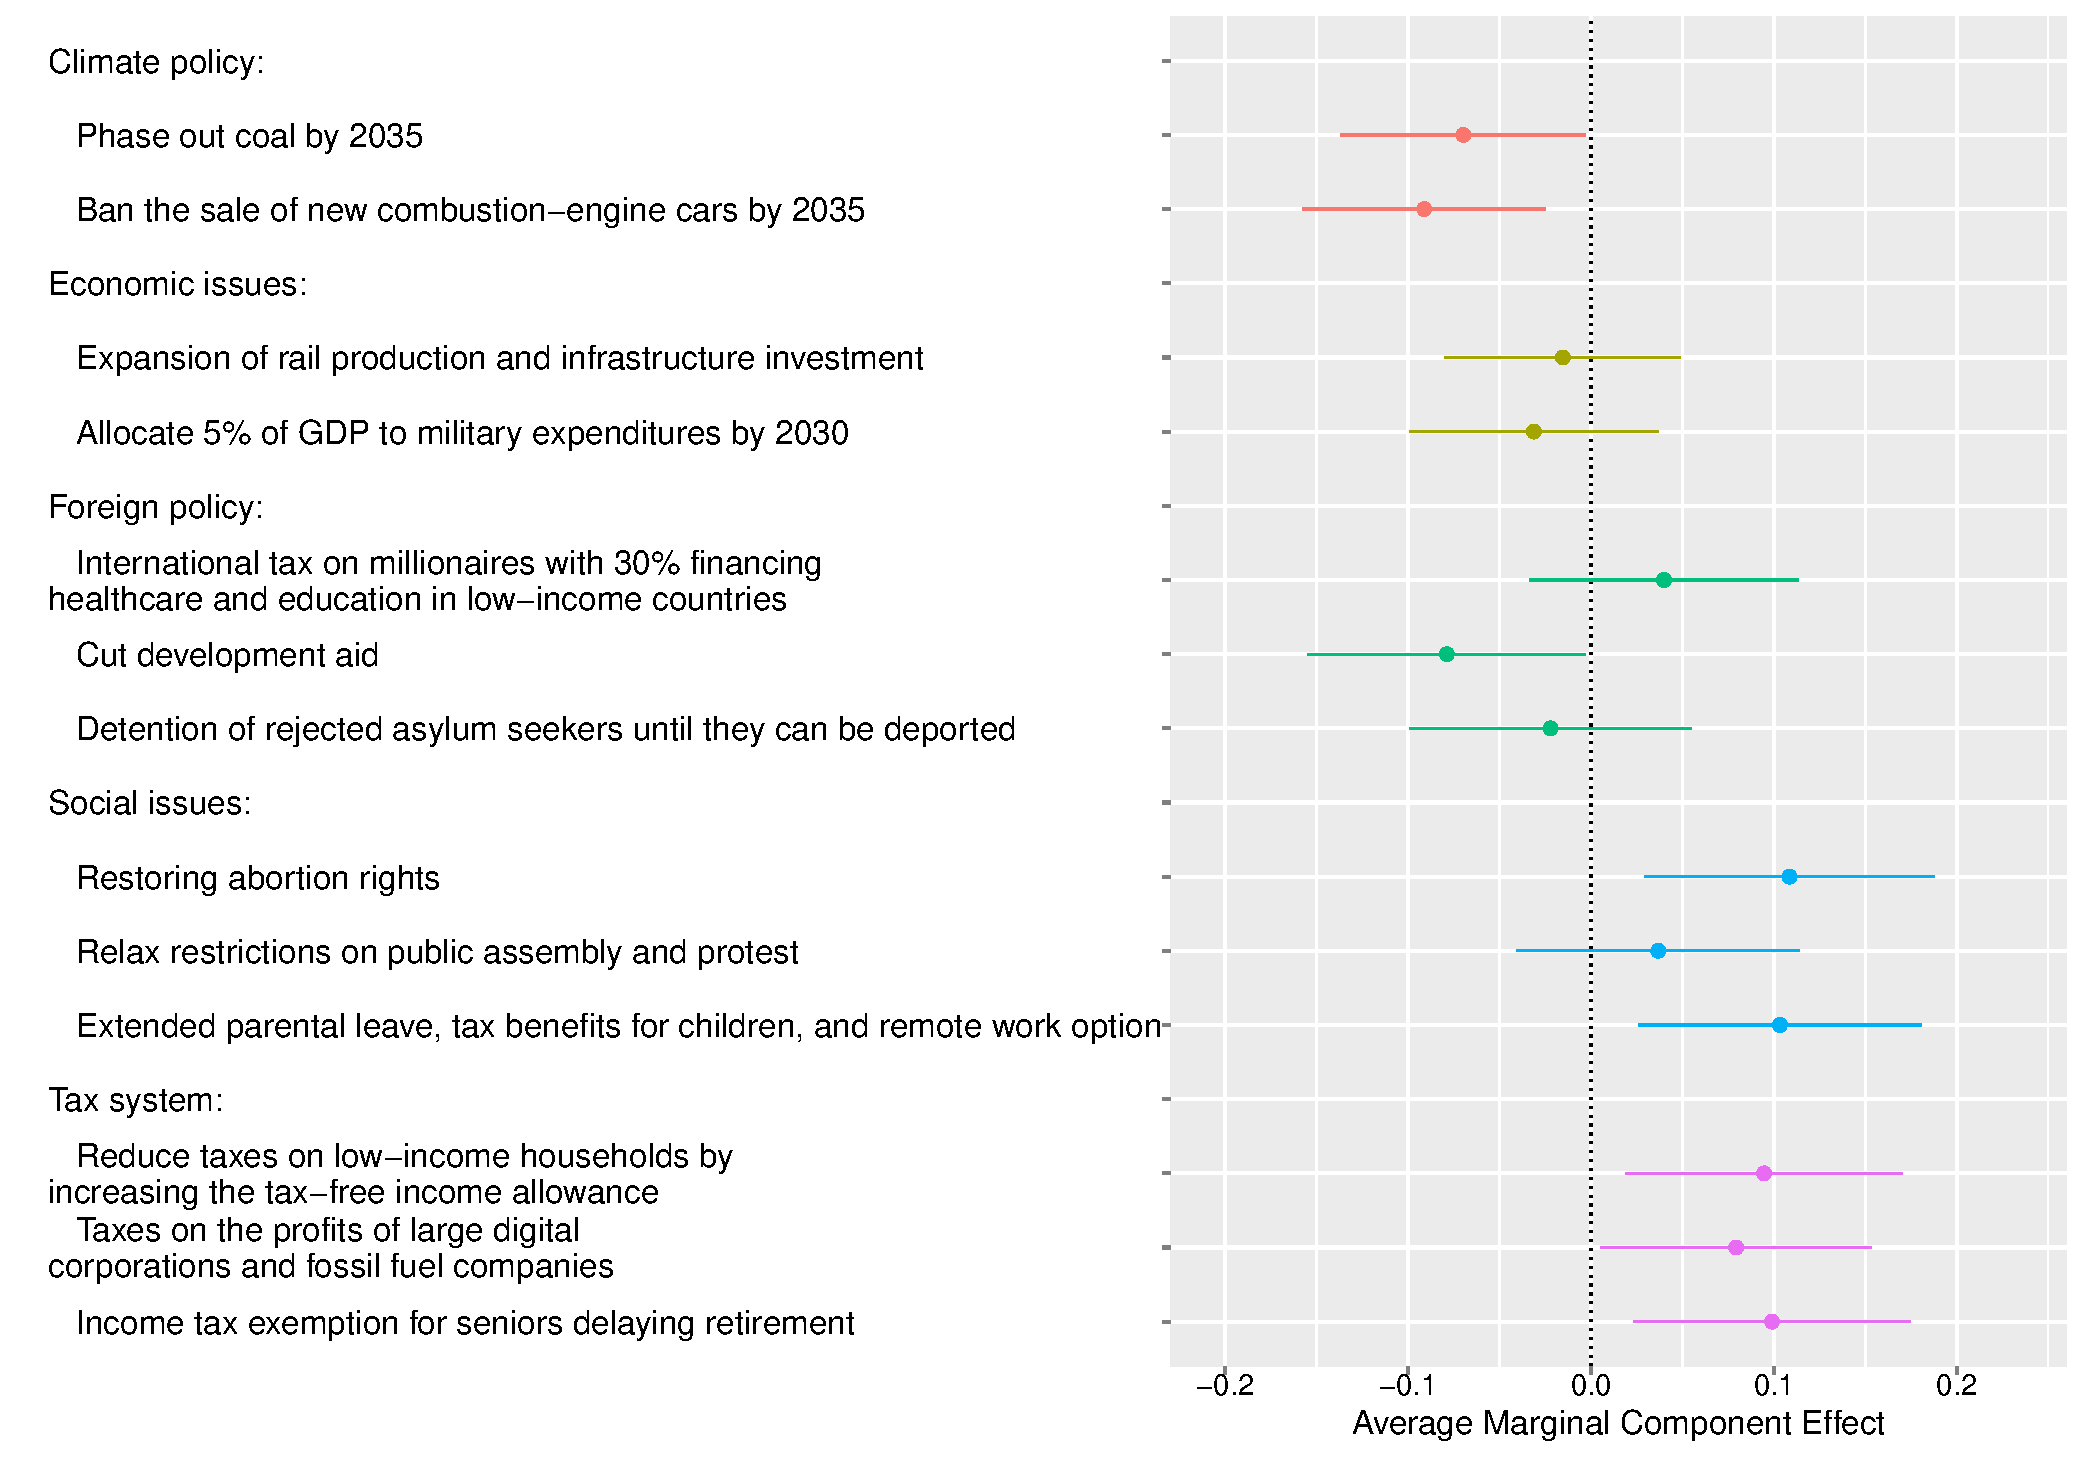
\includegraphics[width=\textwidth]{../figures/all/conjoint_EN-PL.pdf}} 
% \end{figure}

% \begin{figure}[h!]
%     \caption[Conjoint analysis in Spain]{Conjoint analysis in Spain (Average Marginal Component Effect). Cf. Figure \ref{fig:conjoint_ES_original} for Spanish. (Question~\ref{q:conjoint}). \hfill (Back~to~Section~\ref{subsec:conjoint}.)
%     }\label{fig:conjoint_ES}
%     \makebox[\textwidth][c]{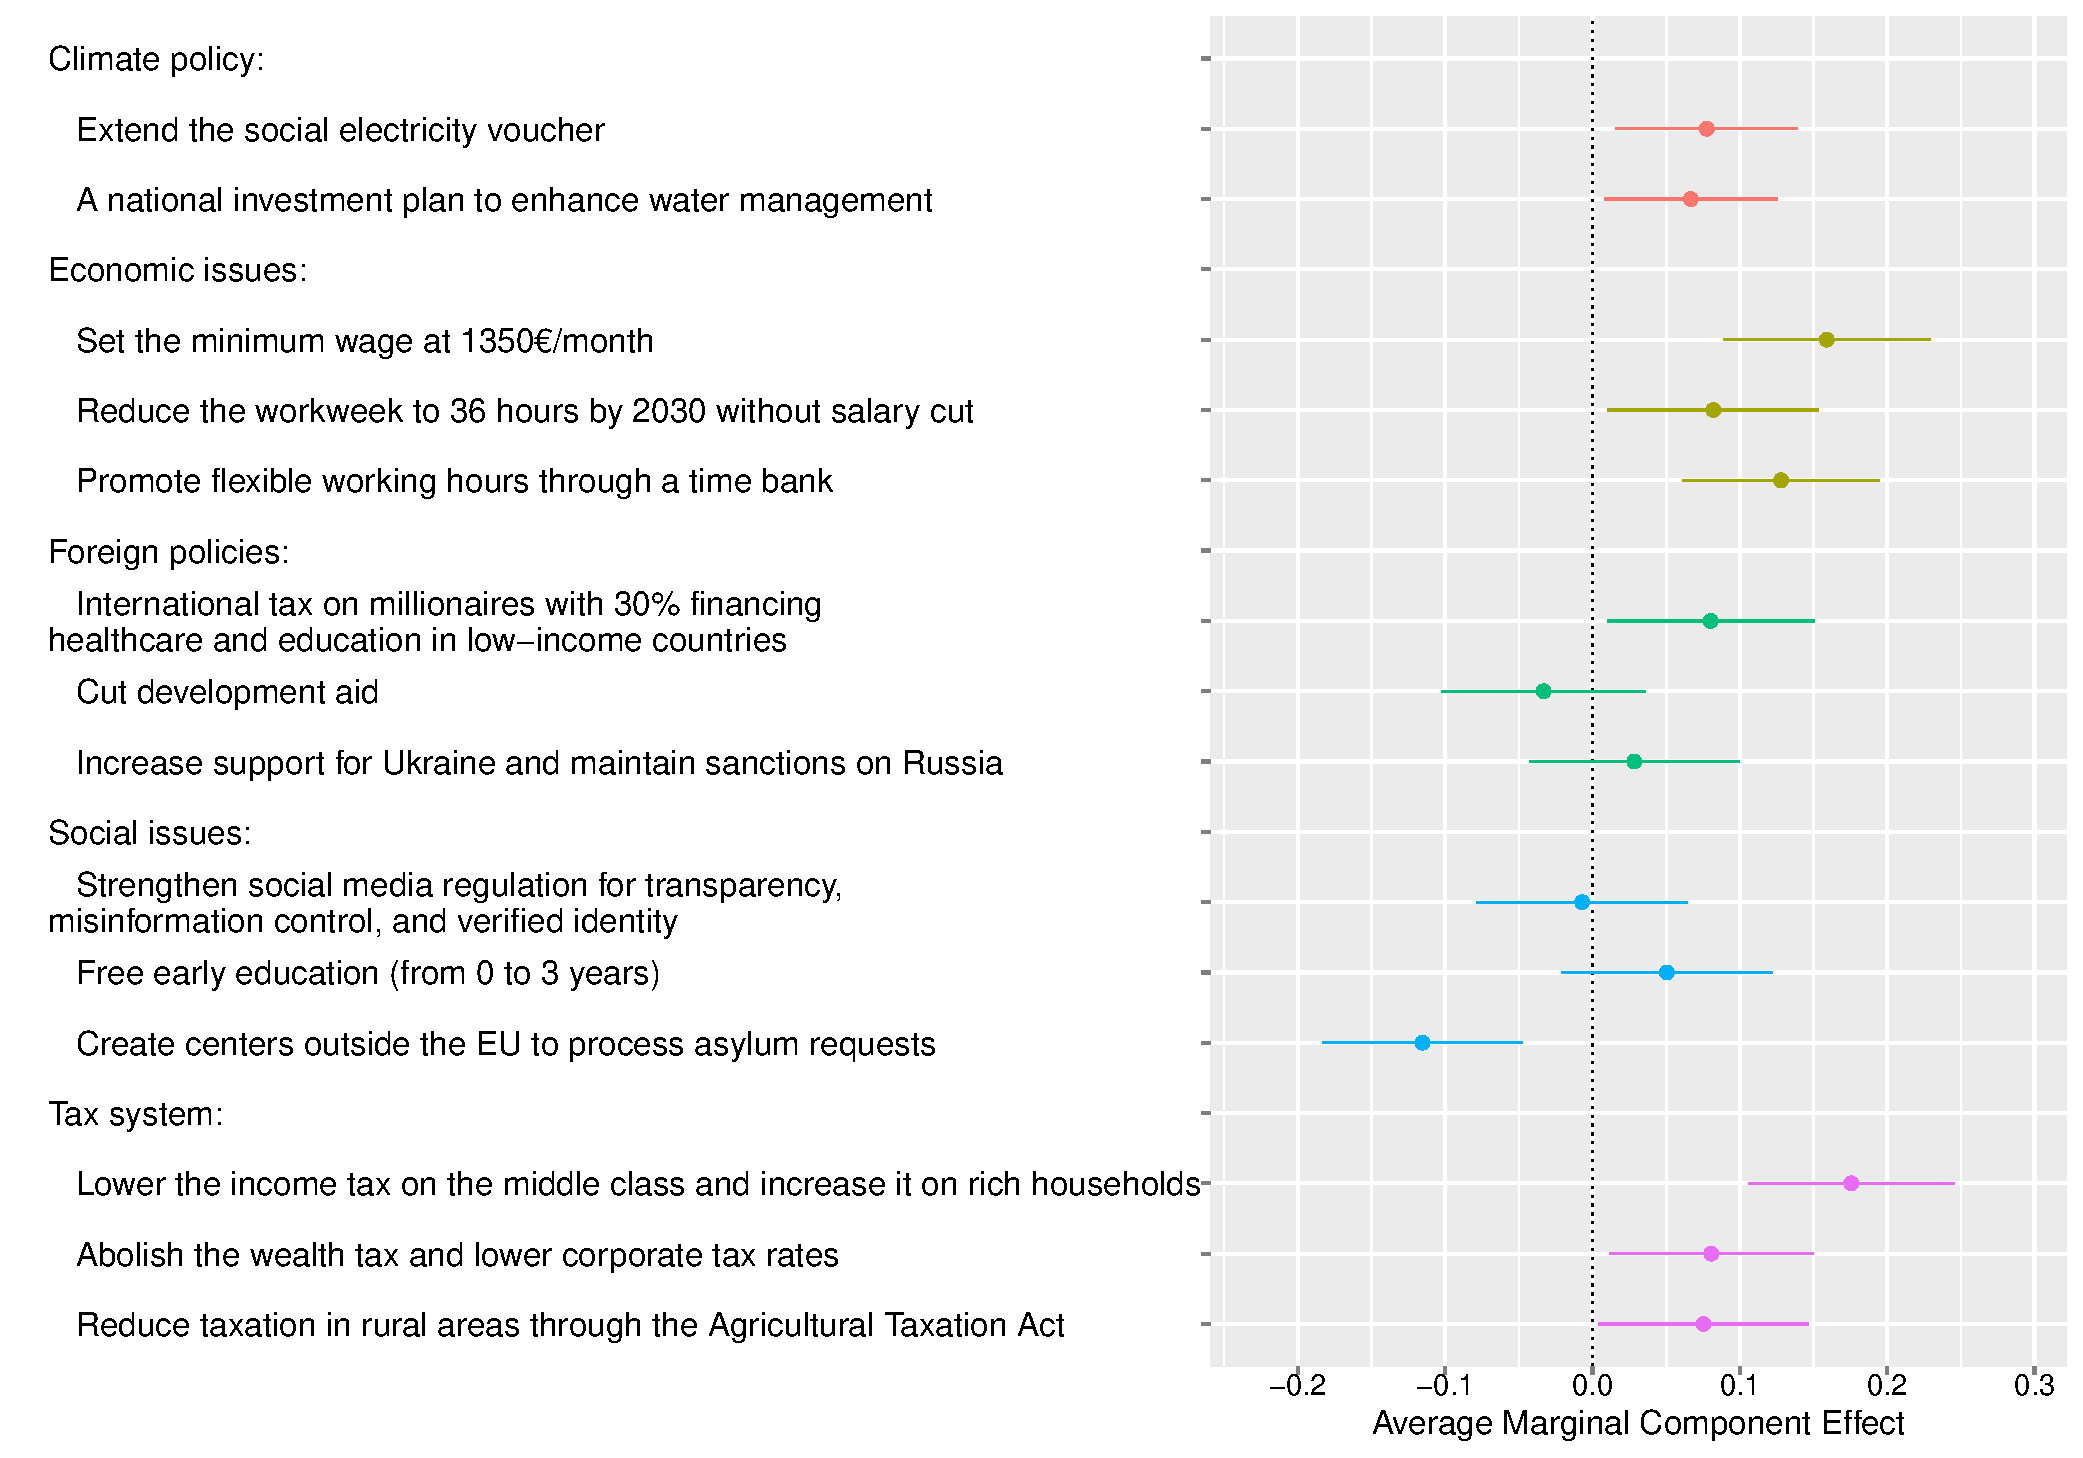
\includegraphics[width=\textwidth]{../figures/all/conjoint_EN-ES.pdf}} 
% \end{figure}

% \begin{figure}[h!]
%     \caption[Conjoint analysis in the UK]{Conjoint analysis in the UK (Average Marginal Component Effect). (Question~\ref{q:conjoint}). \hfill (Back~to~Section~\ref{subsec:conjoint}.)
%     }\label{fig:conjoint_GB}
%     \makebox[\textwidth][c]{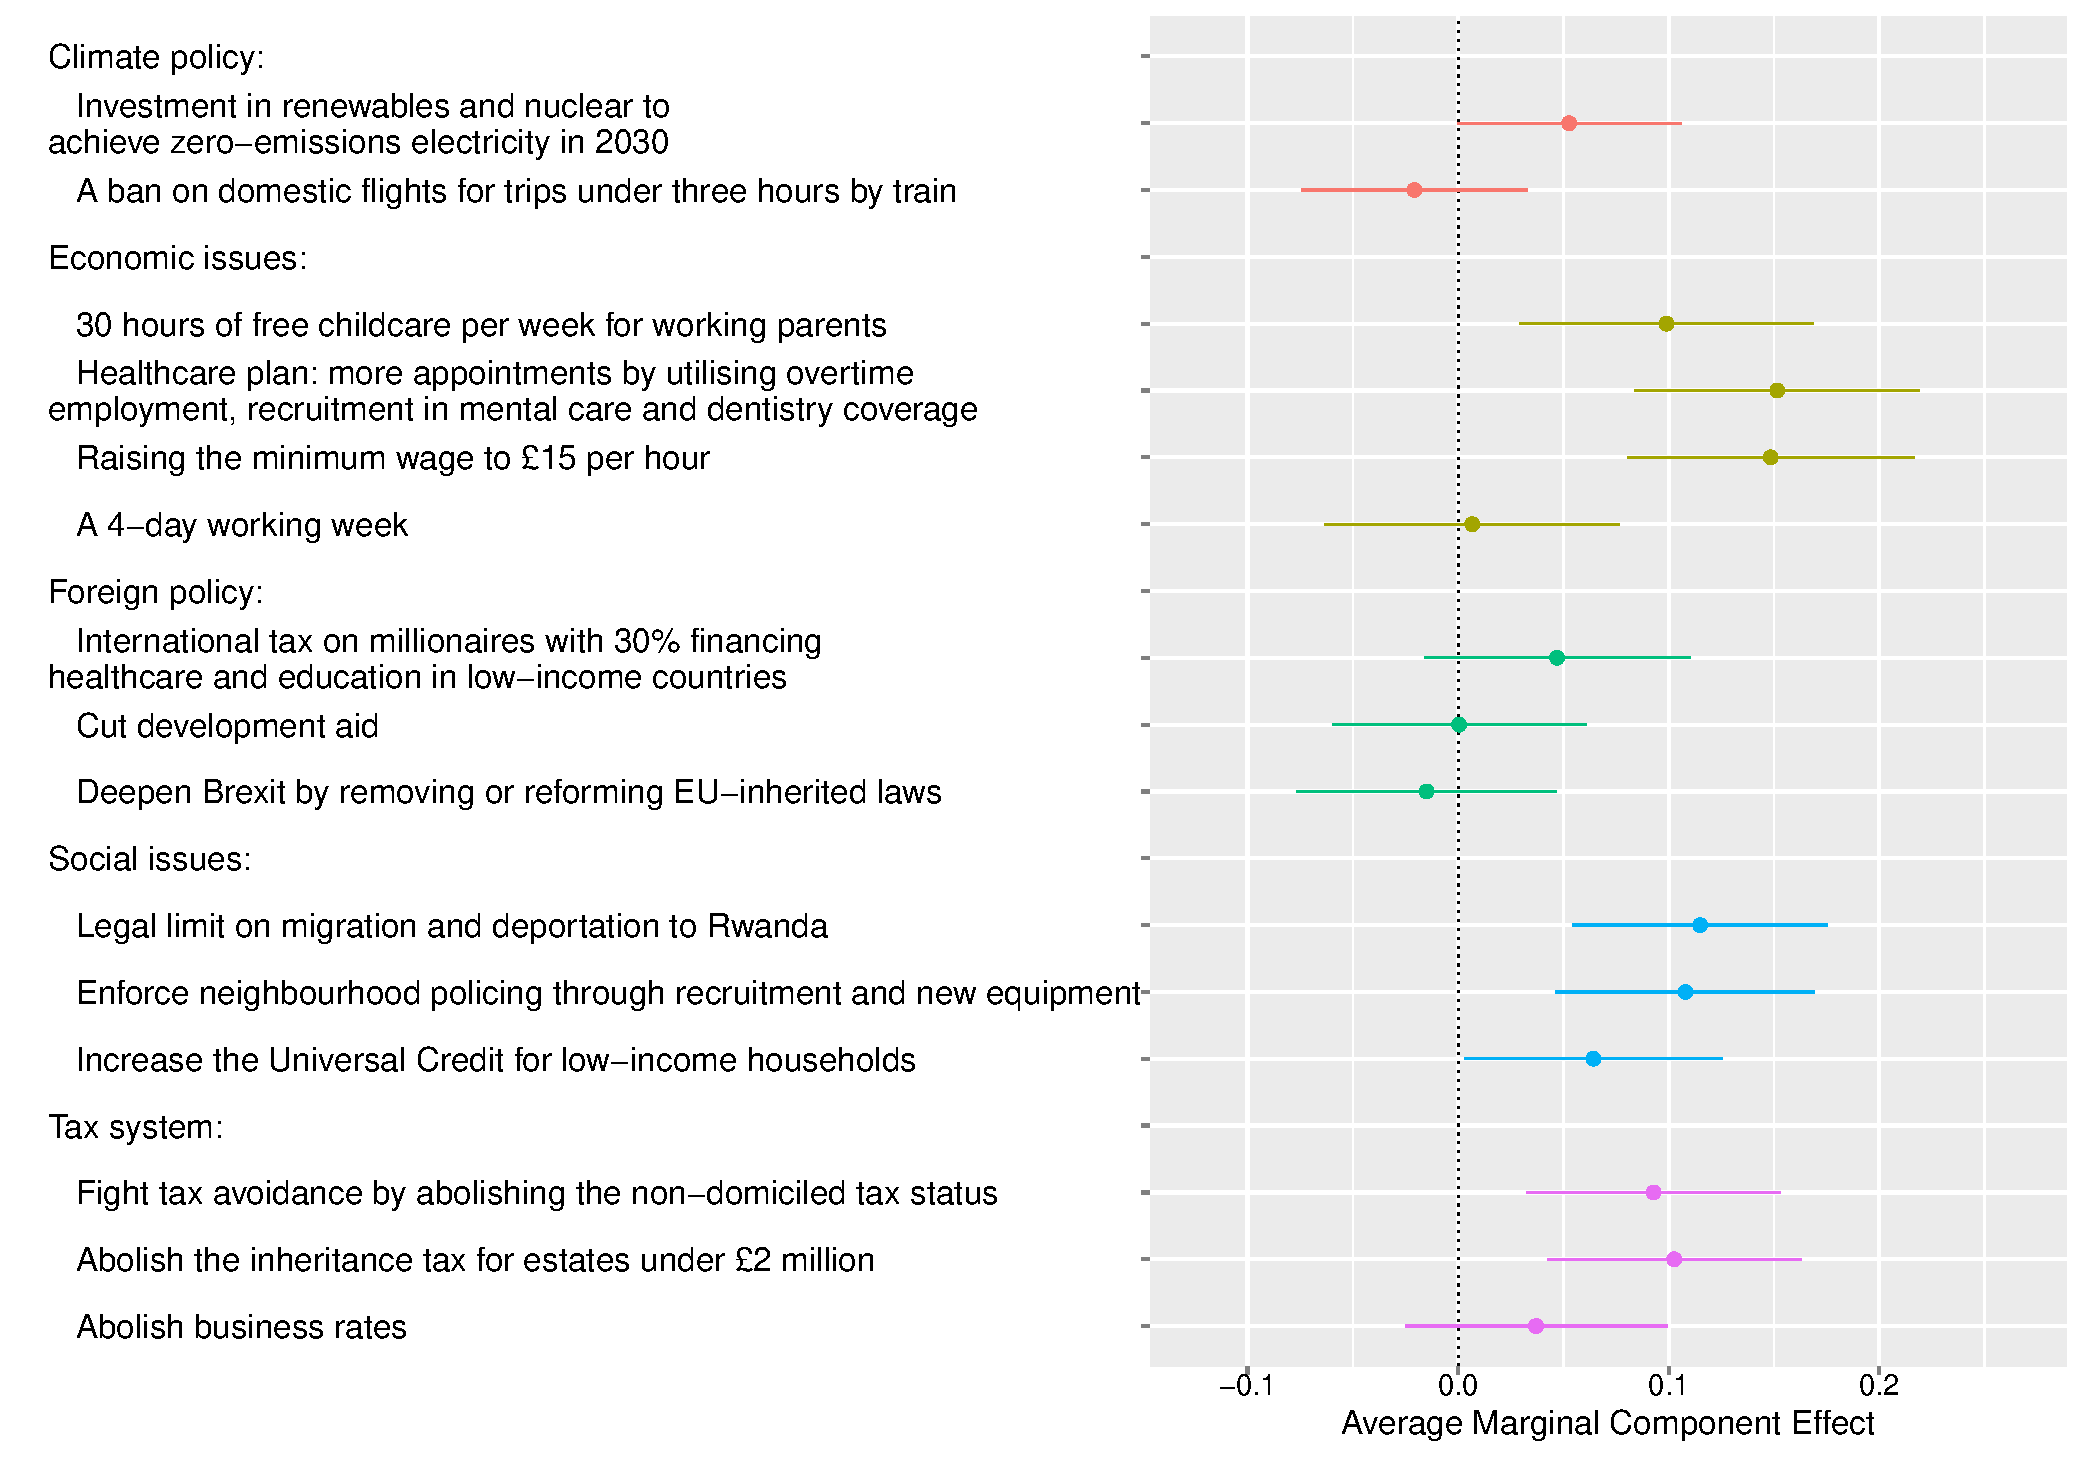
\includegraphics[width=\textwidth]{../figures/all/conjoint_EN-GB.pdf}} 
% \end{figure}

% \begin{figure}[h!]
%     \caption[Conjoint analysis in Switzerland]{Conjoint analysis in Switzerland (Average Marginal Component Effect). (Question~\ref{q:conjoint}). \hfill (Back~to~Section~\ref{subsec:conjoint}.)
%     }\label{fig:conjoint_CH}
%     \makebox[\textwidth][c]{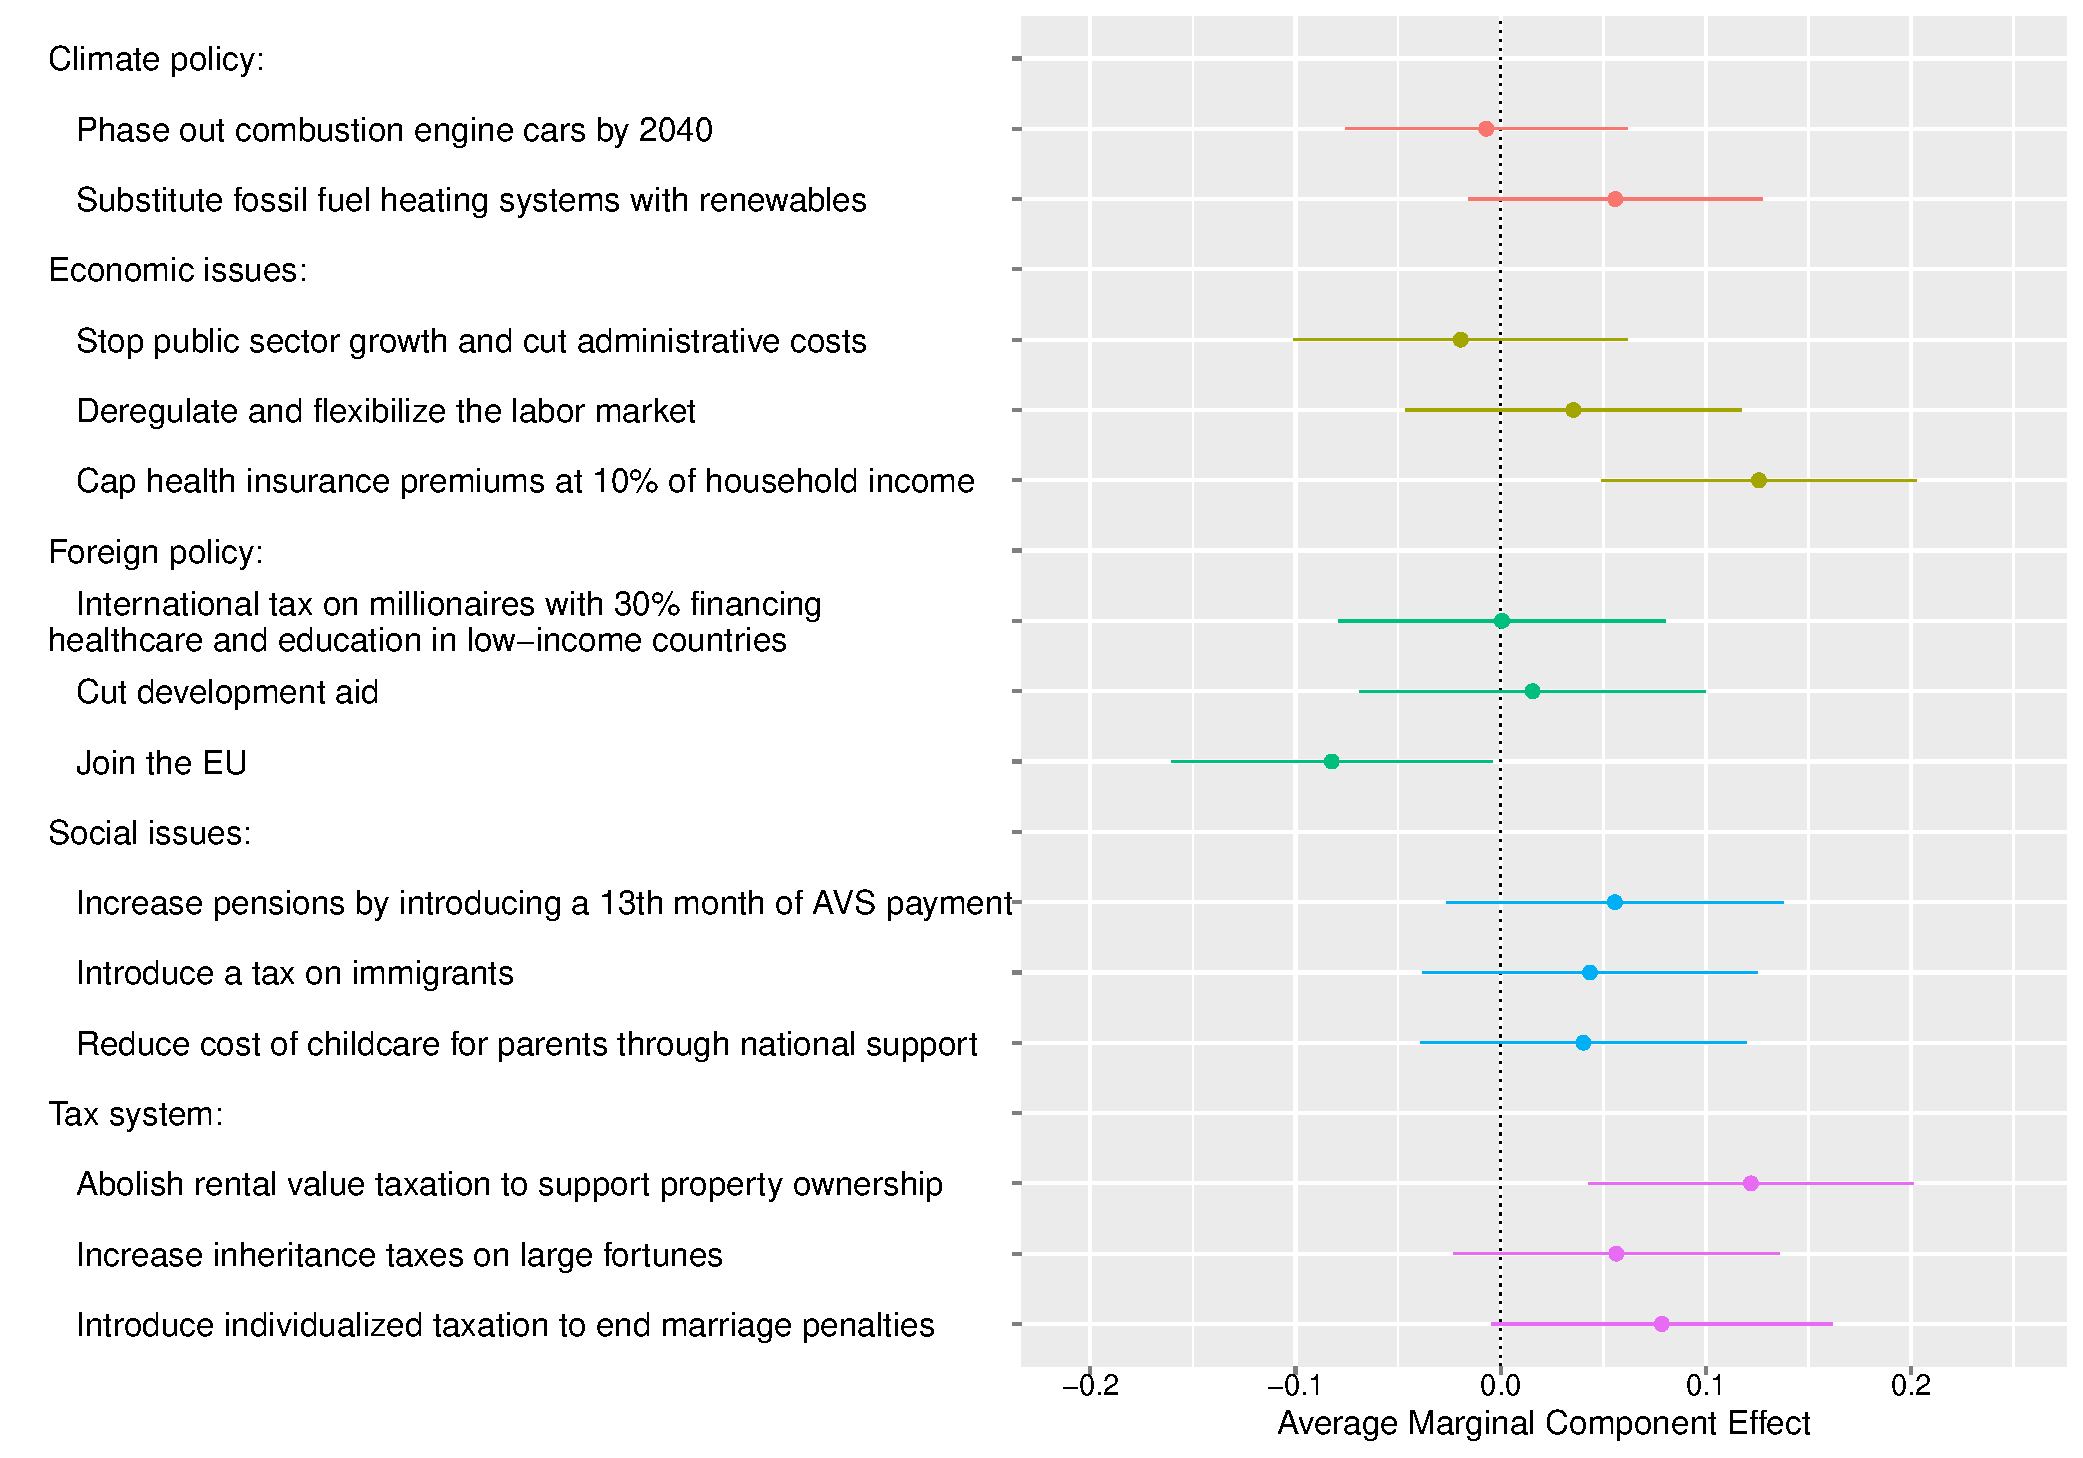
\includegraphics[width=\textwidth]{../figures/all/conjoint_EN-CH.pdf}} 
% \end{figure} 

% \begin{figure}[h!]
%     \caption[Conjoint analysis in Japan]{Conjoint analysis in Japan (Average Marginal Component Effect). (Question~\ref{q:conjoint}). \hfill (Back~to~Section~\ref{subsec:conjoint}.)
%     }\label{fig:conjoint_JP}
%     \makebox[\textwidth][c]{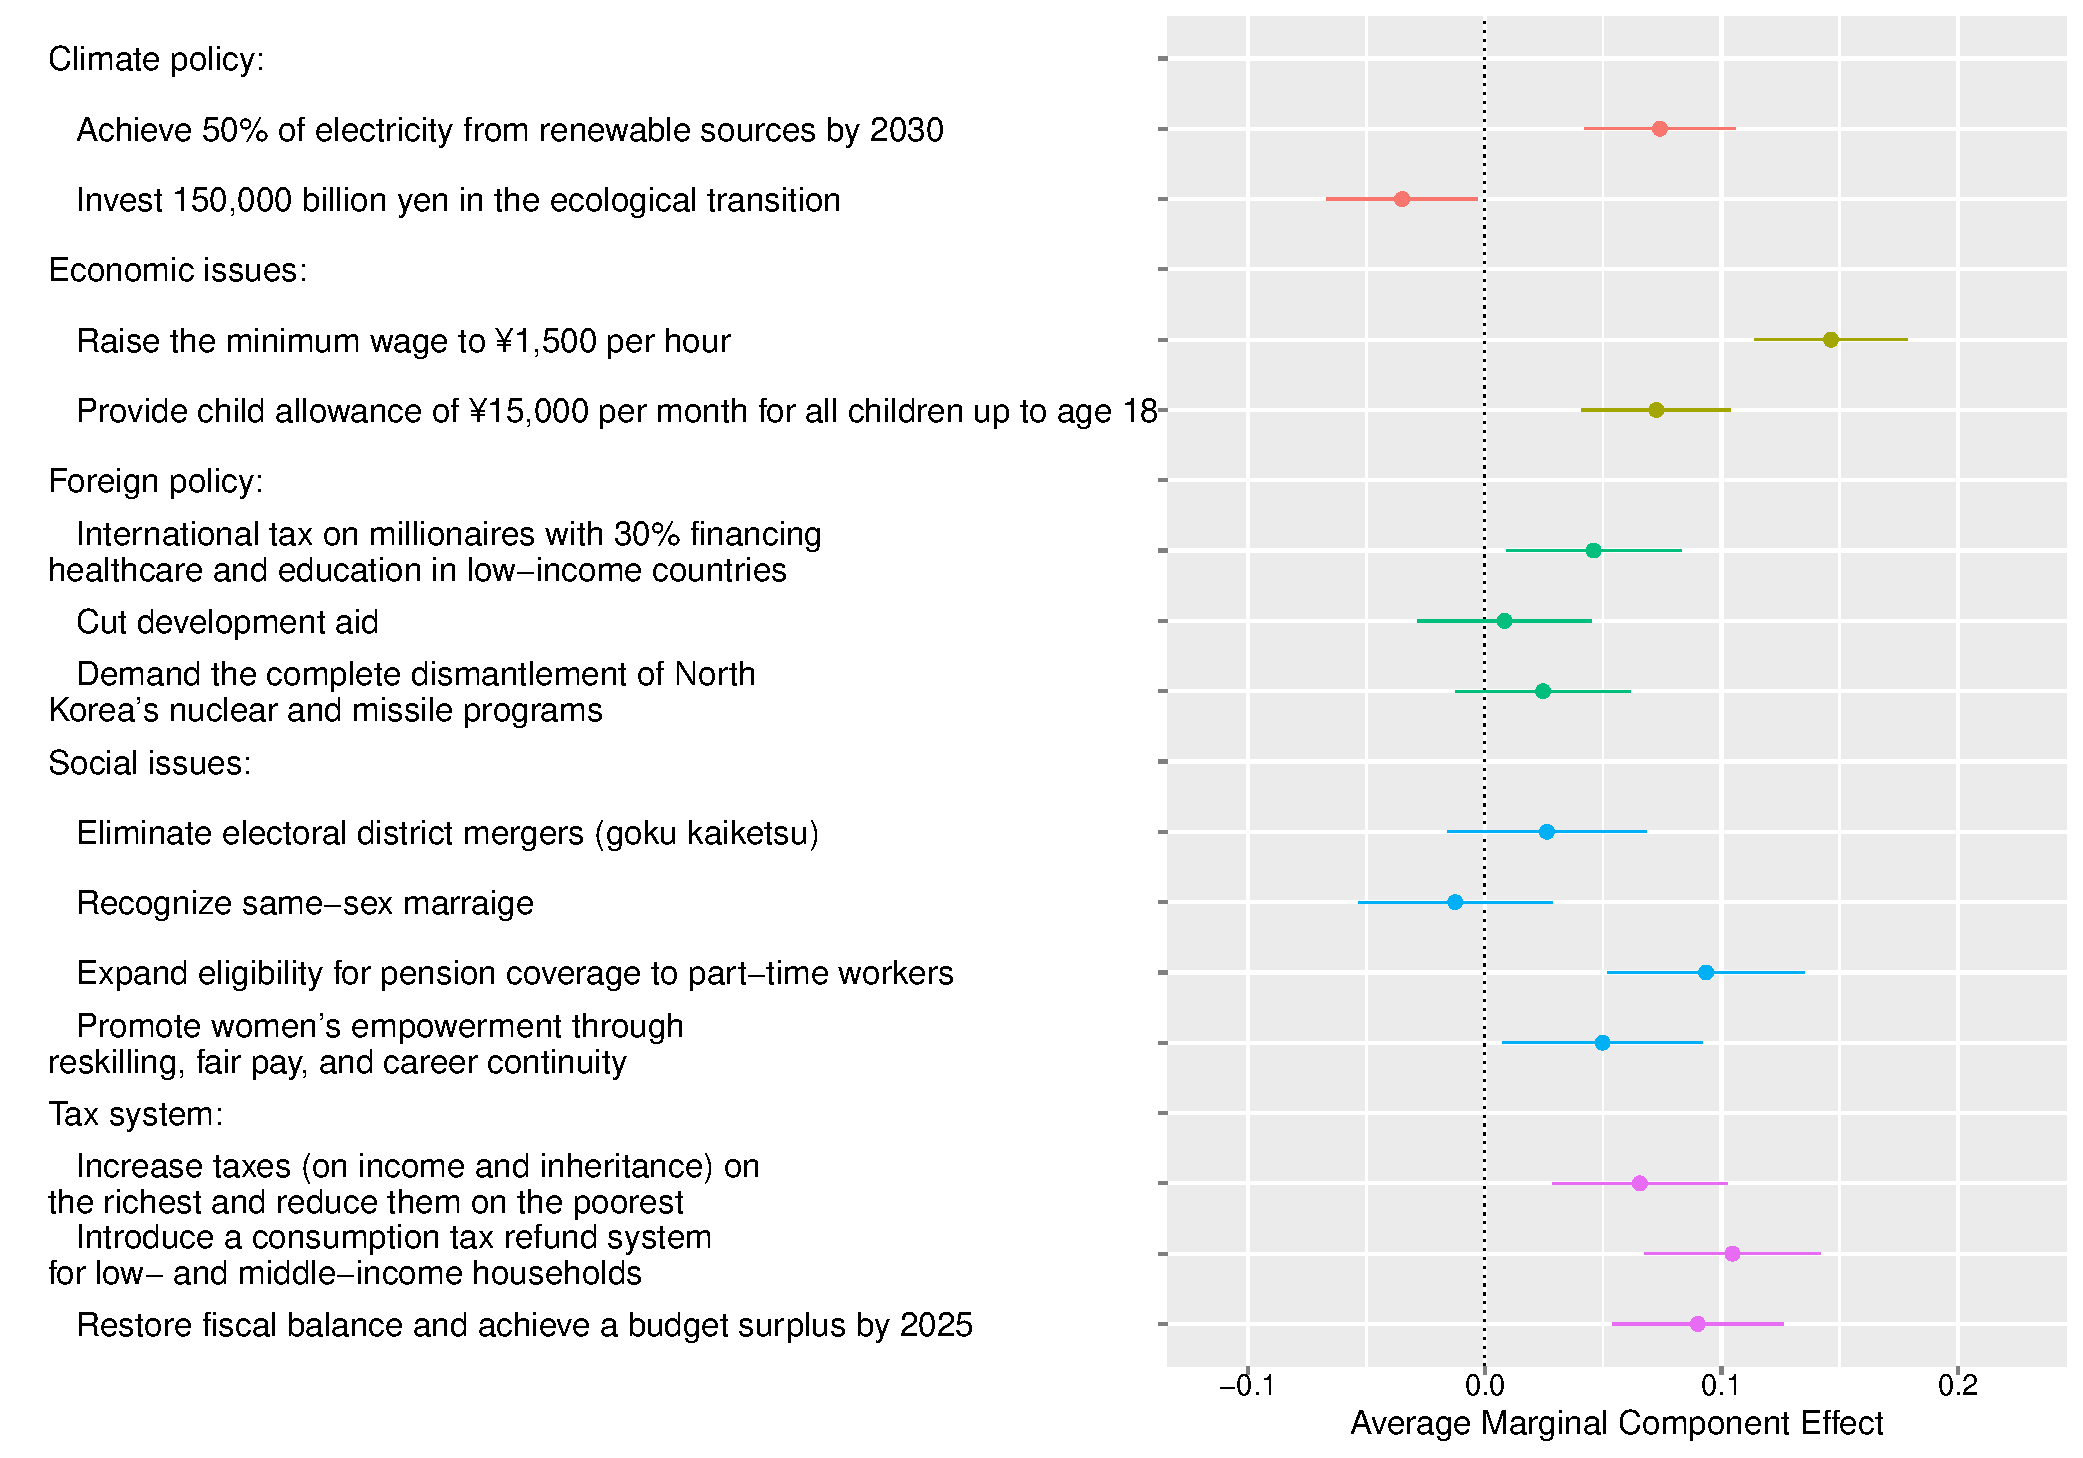
\includegraphics[width=\textwidth]{../figures/all/conjoint_EN-JA.pdf}} 
% \end{figure} 
\begin{figure}[h!]
    \caption[Conjoint analysis in the U.S.]{Conjoint analysis in the U.S. (Average Marginal Component Effect). (Question~\ref{q:conjoint}). \hfill (Back~to~Section~\ref{subsec:conjoint}.)
    }\label{fig:conjoint_US}
    \makebox[\textwidth][c]{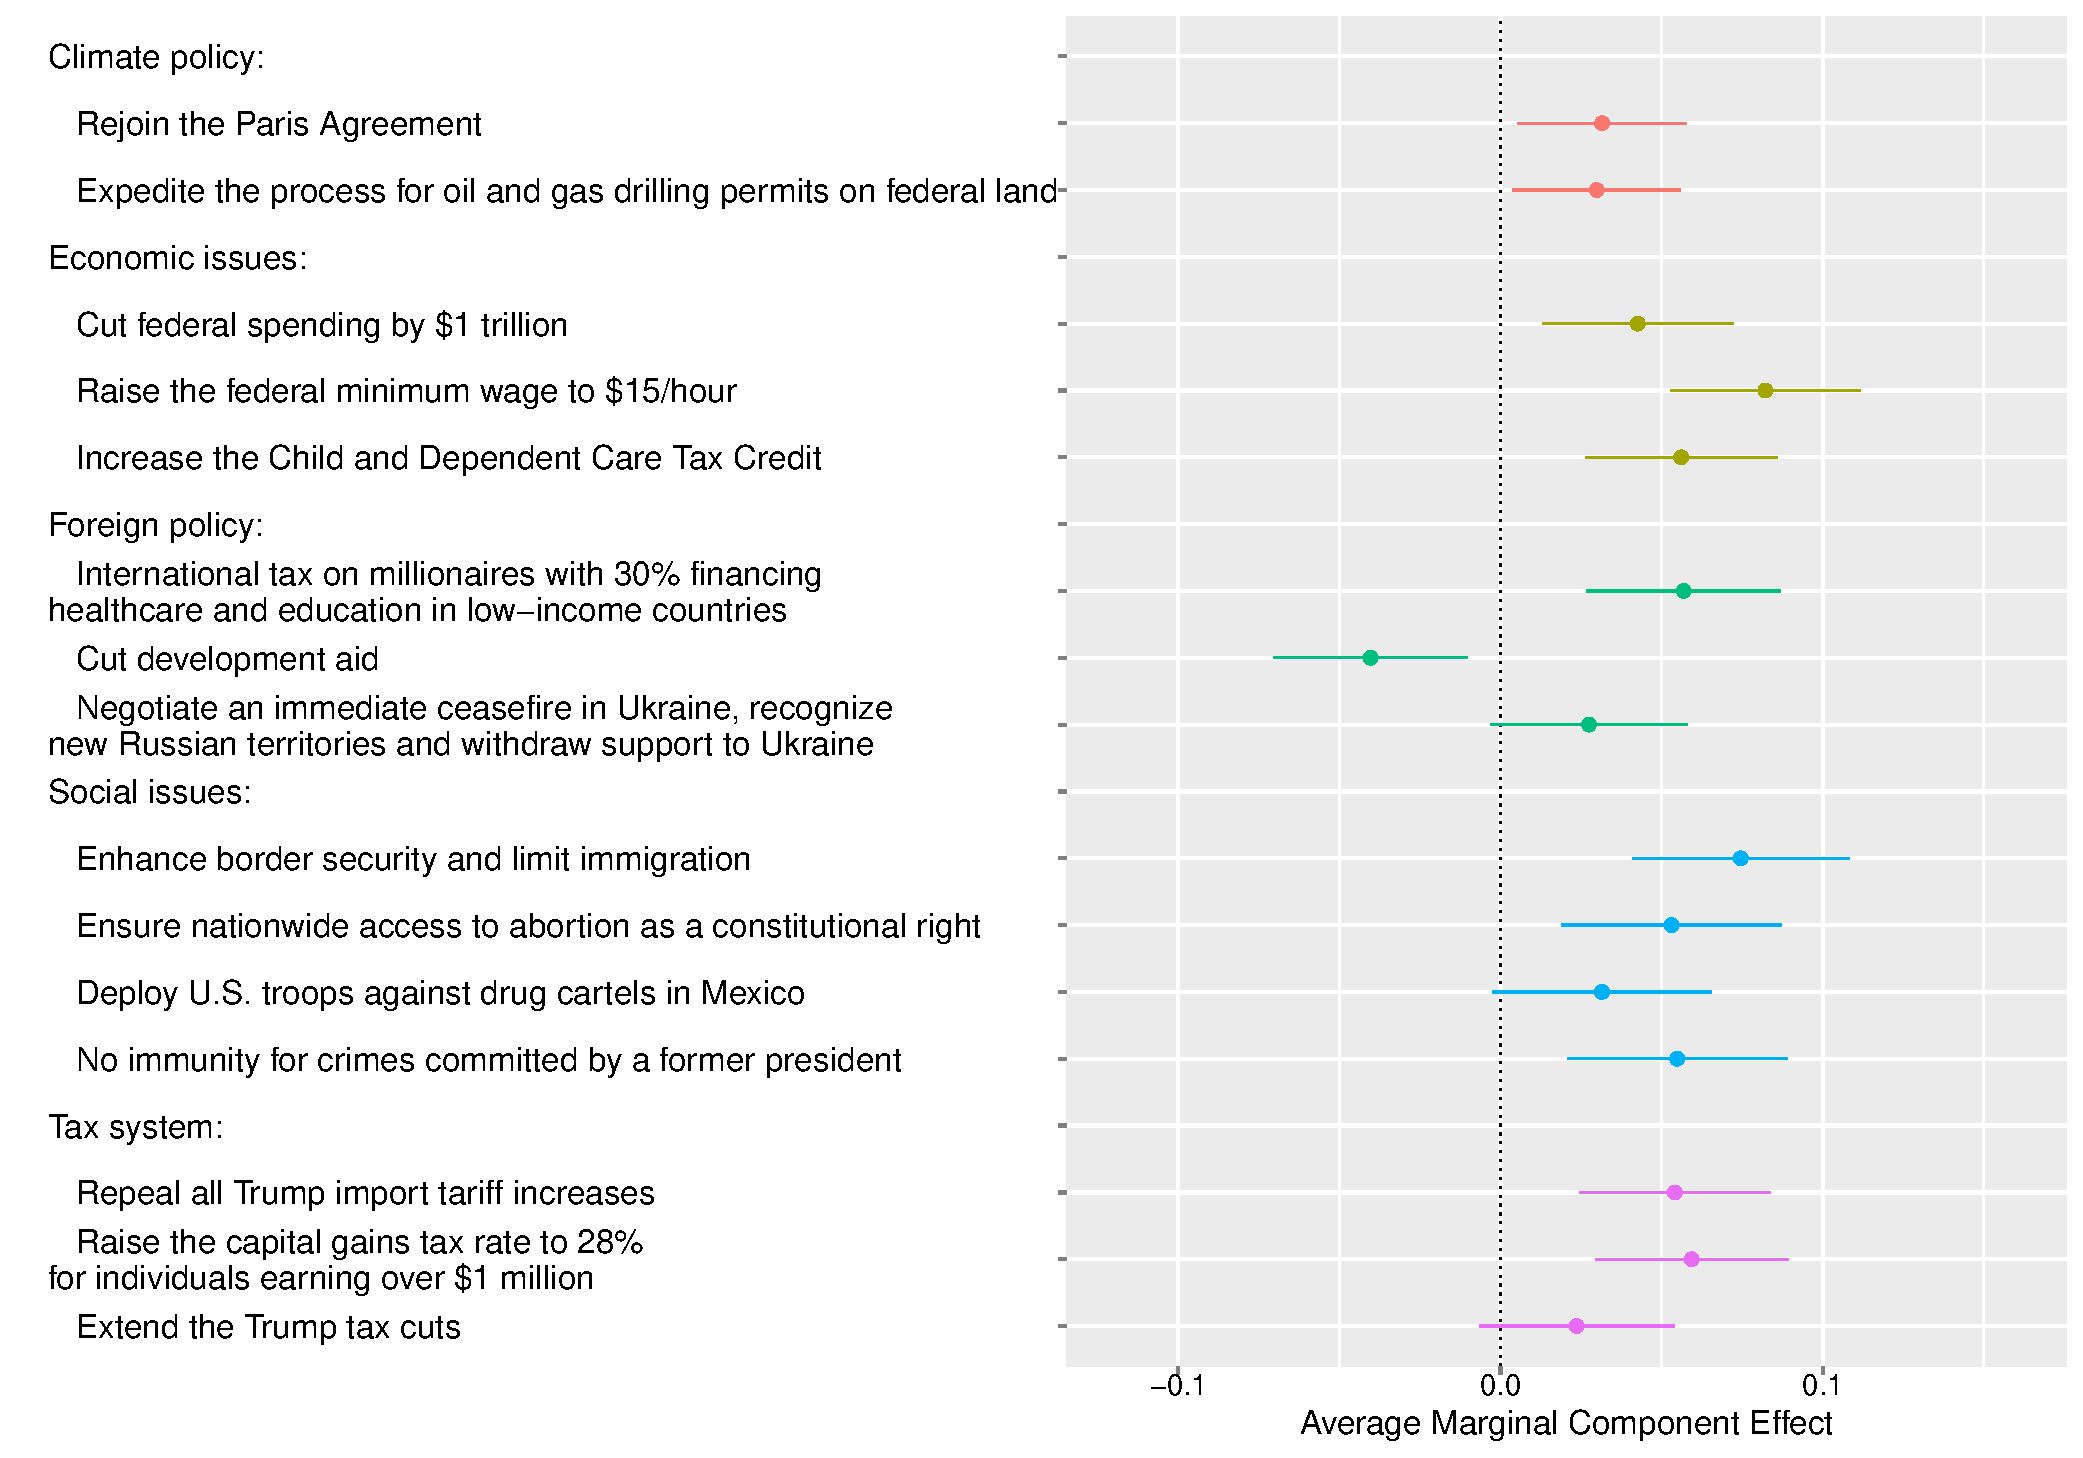
\includegraphics[width=\textwidth]{../figures/all/conjoint_EN.pdf}} 
\end{figure} 

% \begin{figure}[h!]
%     \caption[Conjoint analysis in France (French)]{Conjoint analysis in France (in French, cf. Figure \ref{fig:conjoint_FR} for English). (Question~\ref{q:conjoint}). \hfill (Back~to~Section~\ref{subsec:conjoint}.)
%     }\label{fig:conjoint_FR_original}
%     \makebox[\textwidth][c]{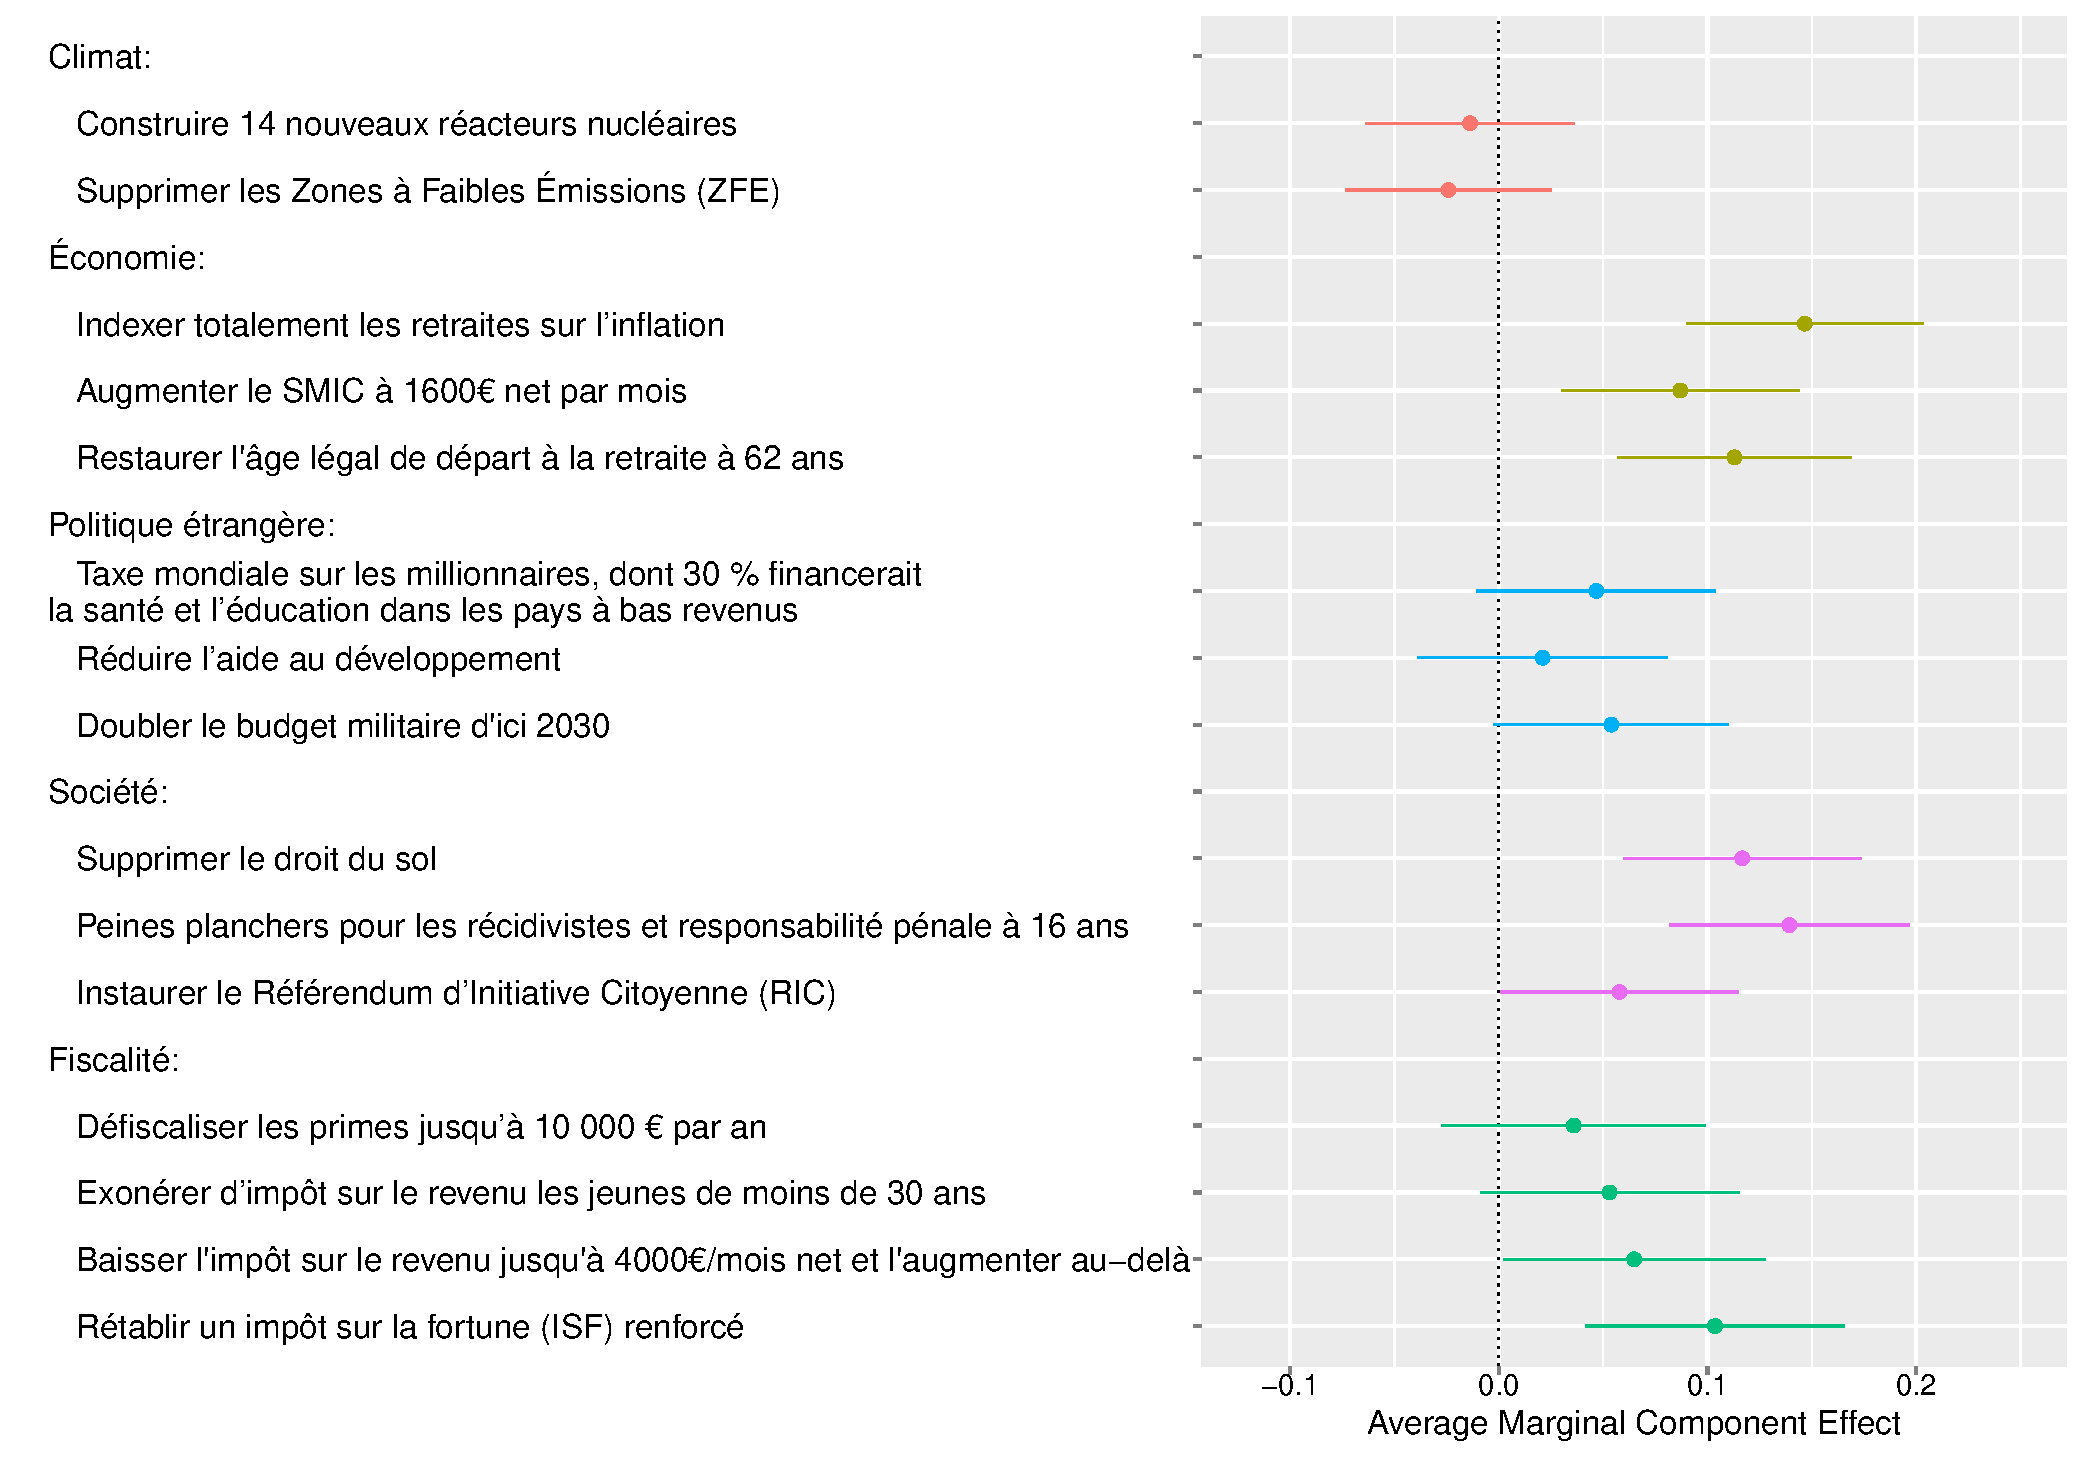
\includegraphics[width=\textwidth]{../figures/all/conjoint_FR.pdf}} 
% \end{figure}

% \begin{figure}[h!]
%     \caption[Conjoint analysis in Germany (German)]{Conjoint analysis in Germany (in German, cf. Figure \ref{fig:conjoint_DE} for English). (Question~\ref{q:conjoint}). \hfill (Back~to~Section~\ref{subsec:conjoint}.)
%     }\label{fig:conjoint_DE_original}
%     \makebox[\textwidth][c]{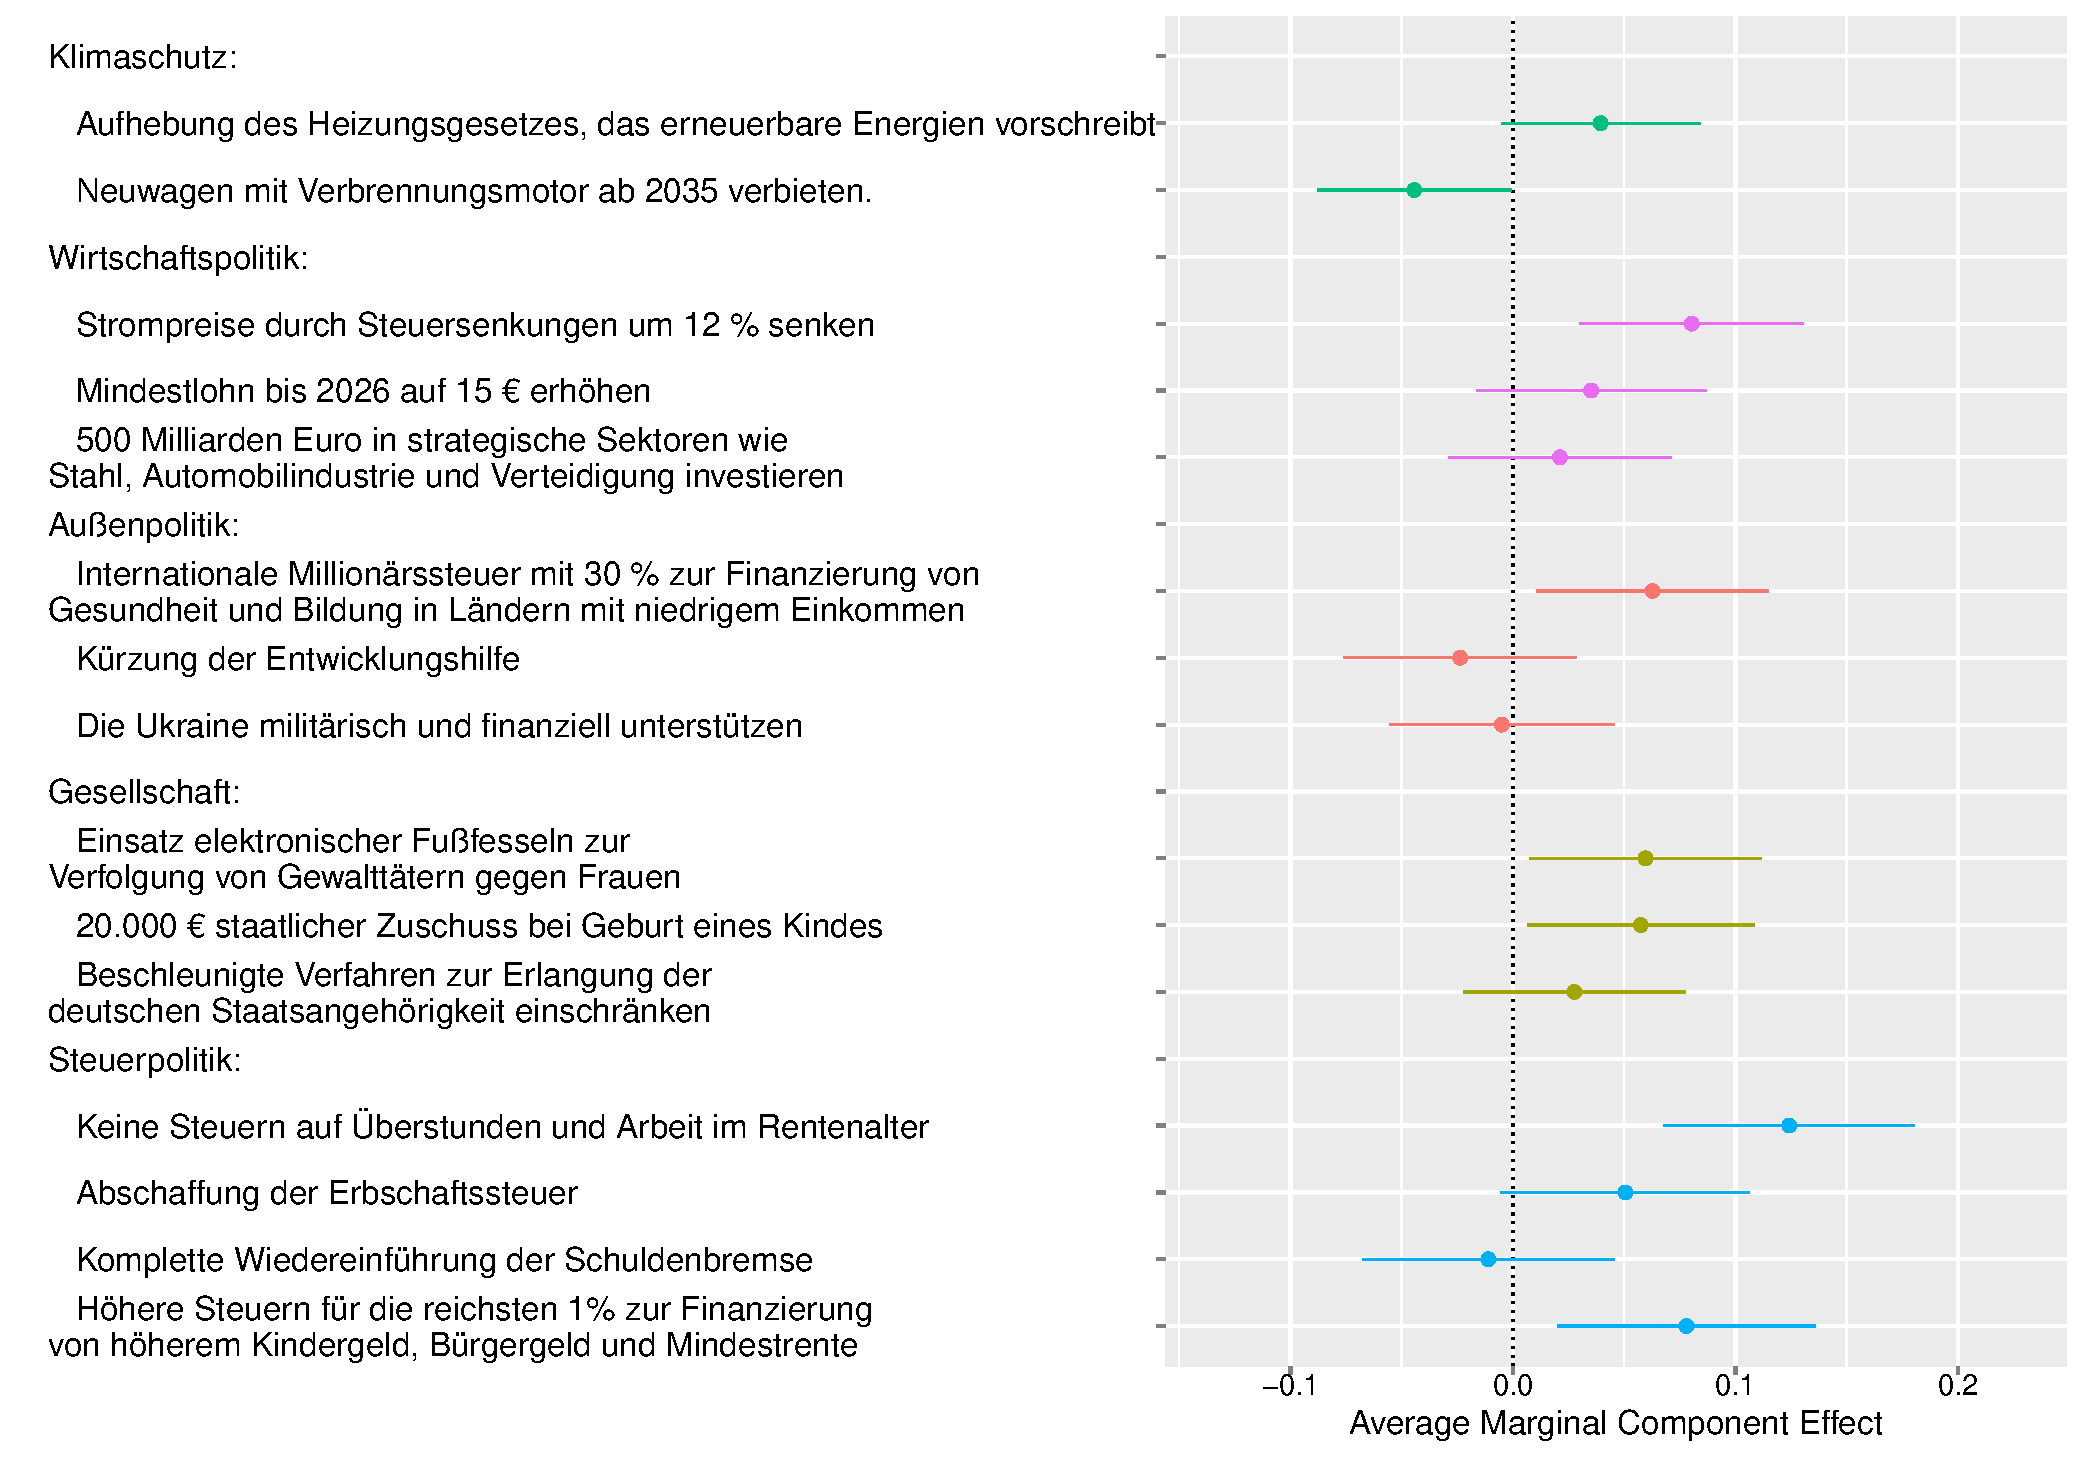
\includegraphics[width=\textwidth]{../figures/all/conjoint_DE.pdf}} 
% \end{figure}

% \begin{figure}[h!]
%     \caption[Conjoint analysis in Italy (Italian)]{Conjoint analysis in Italy (in Italian, cf. Figure \ref{fig:conjoint_IT} for English). (Question~\ref{q:conjoint}). \hfill (Back~to~Section~\ref{subsec:conjoint}.)
%     }\label{fig:conjoint_IT_original}
%     \makebox[\textwidth][c]{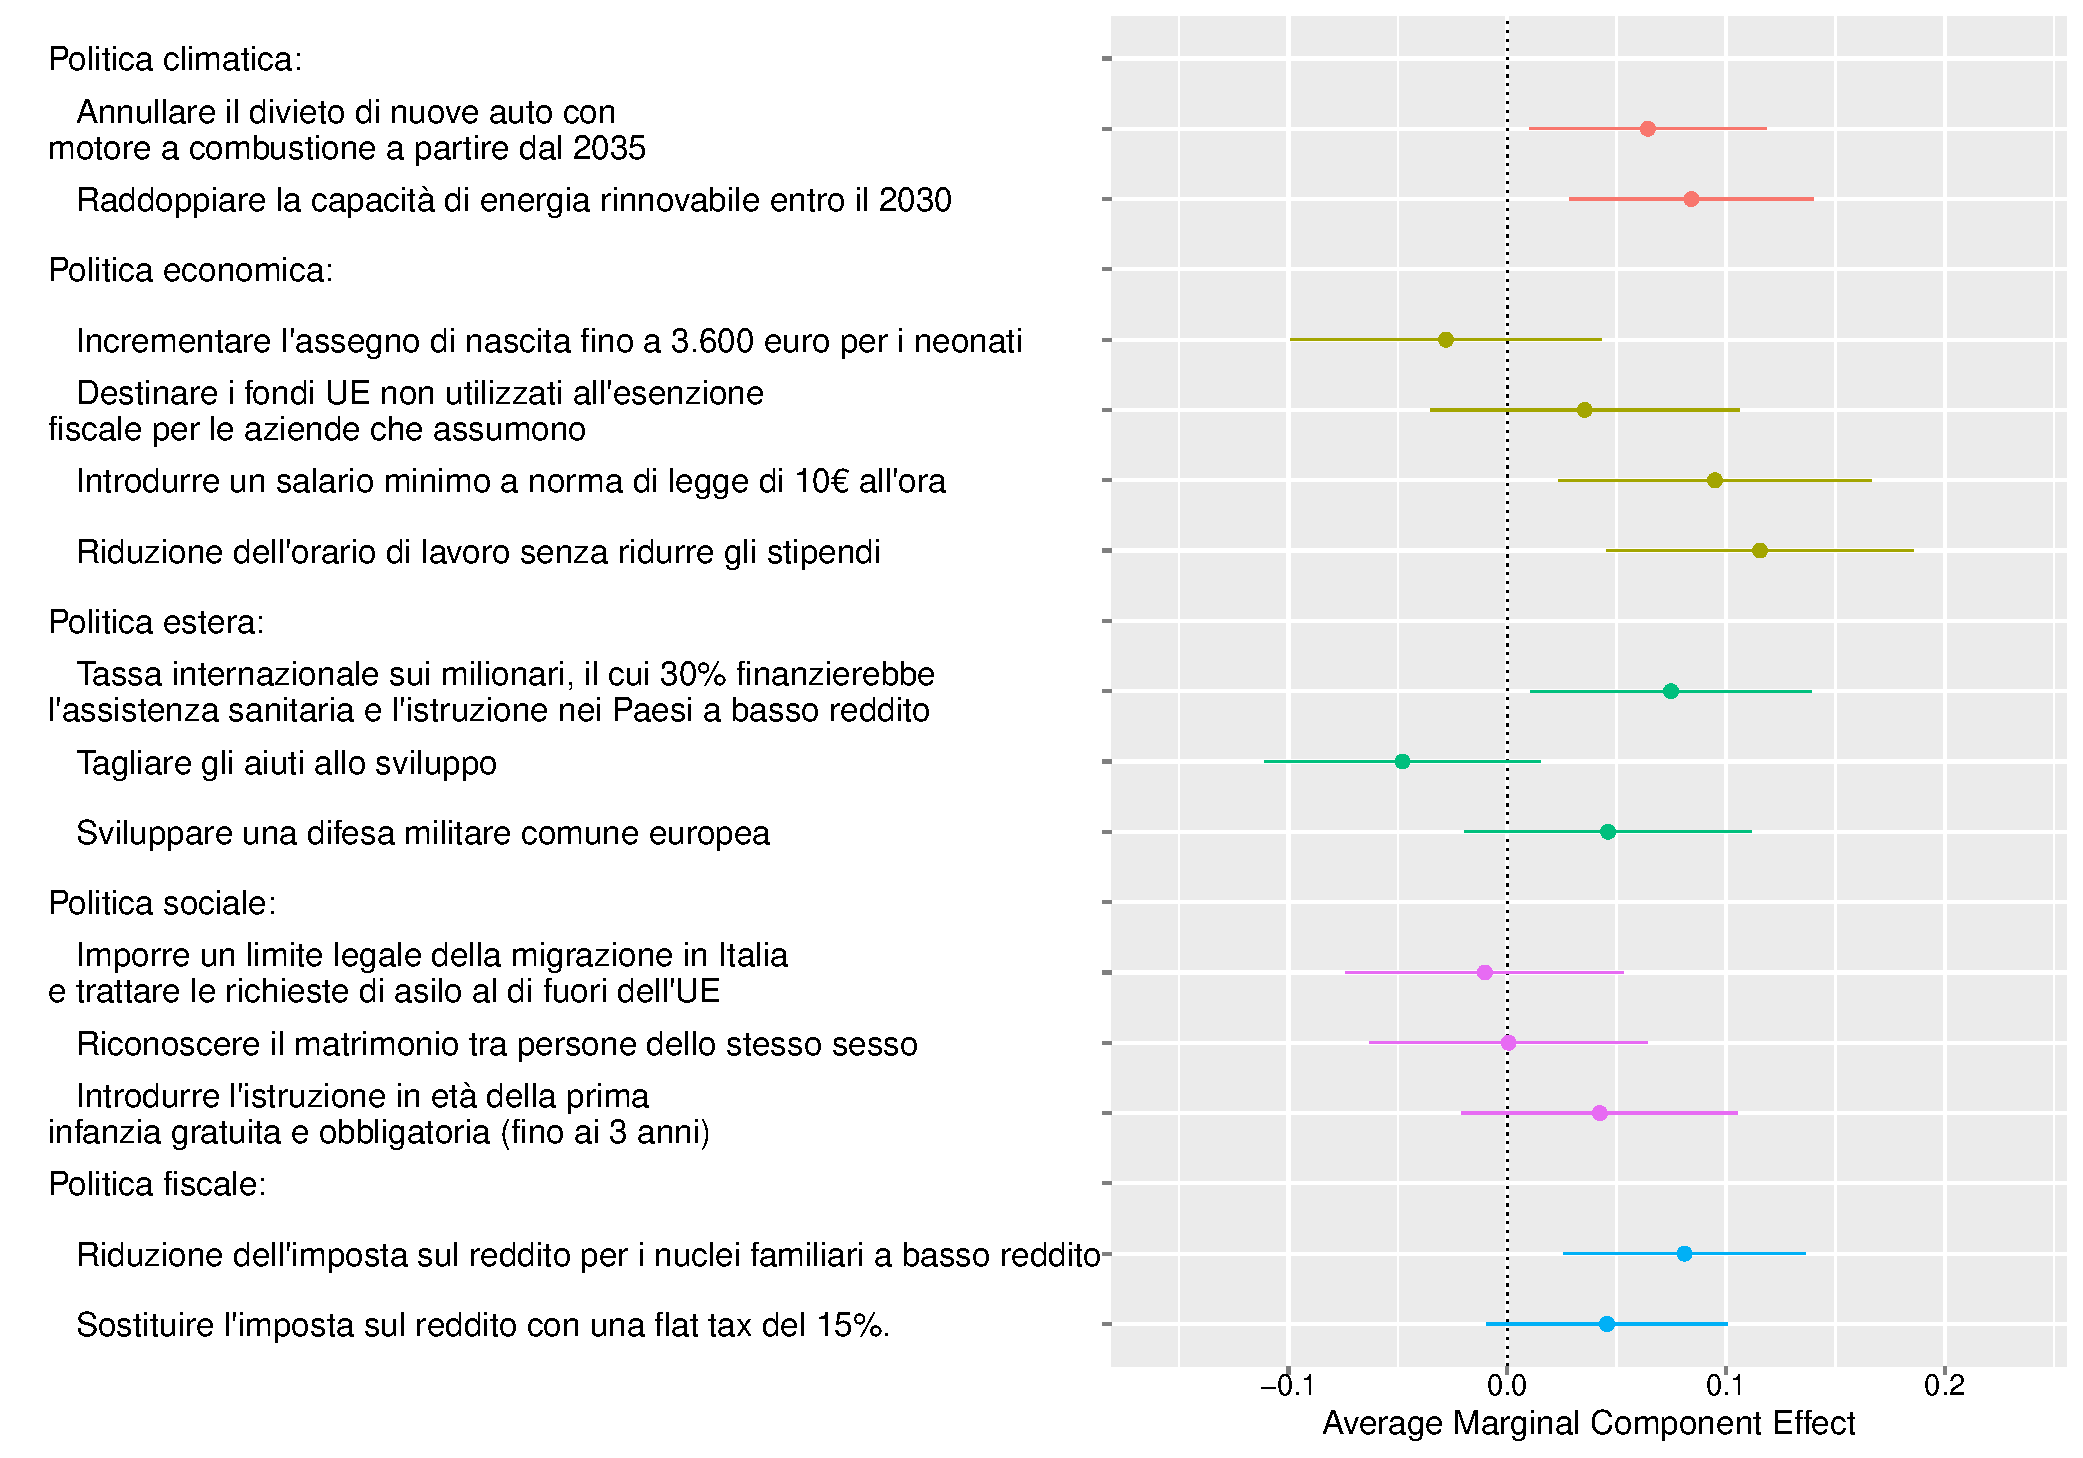
\includegraphics[width=\textwidth]{../figures/all/conjoint_IT.pdf}} 
% \end{figure}

% \begin{figure}[h!]
%     \caption[Conjoint analysis in Poland (Polish)]{Conjoint analysis in Poland (in Polish, cf. Figure \ref{fig:conjoint_PL} for English). (Question~\ref{q:conjoint}). \hfill (Back~to~Section~\ref{subsec:conjoint}.)
%     }\label{fig:conjoint_PL_original}
%     \makebox[\textwidth][c]{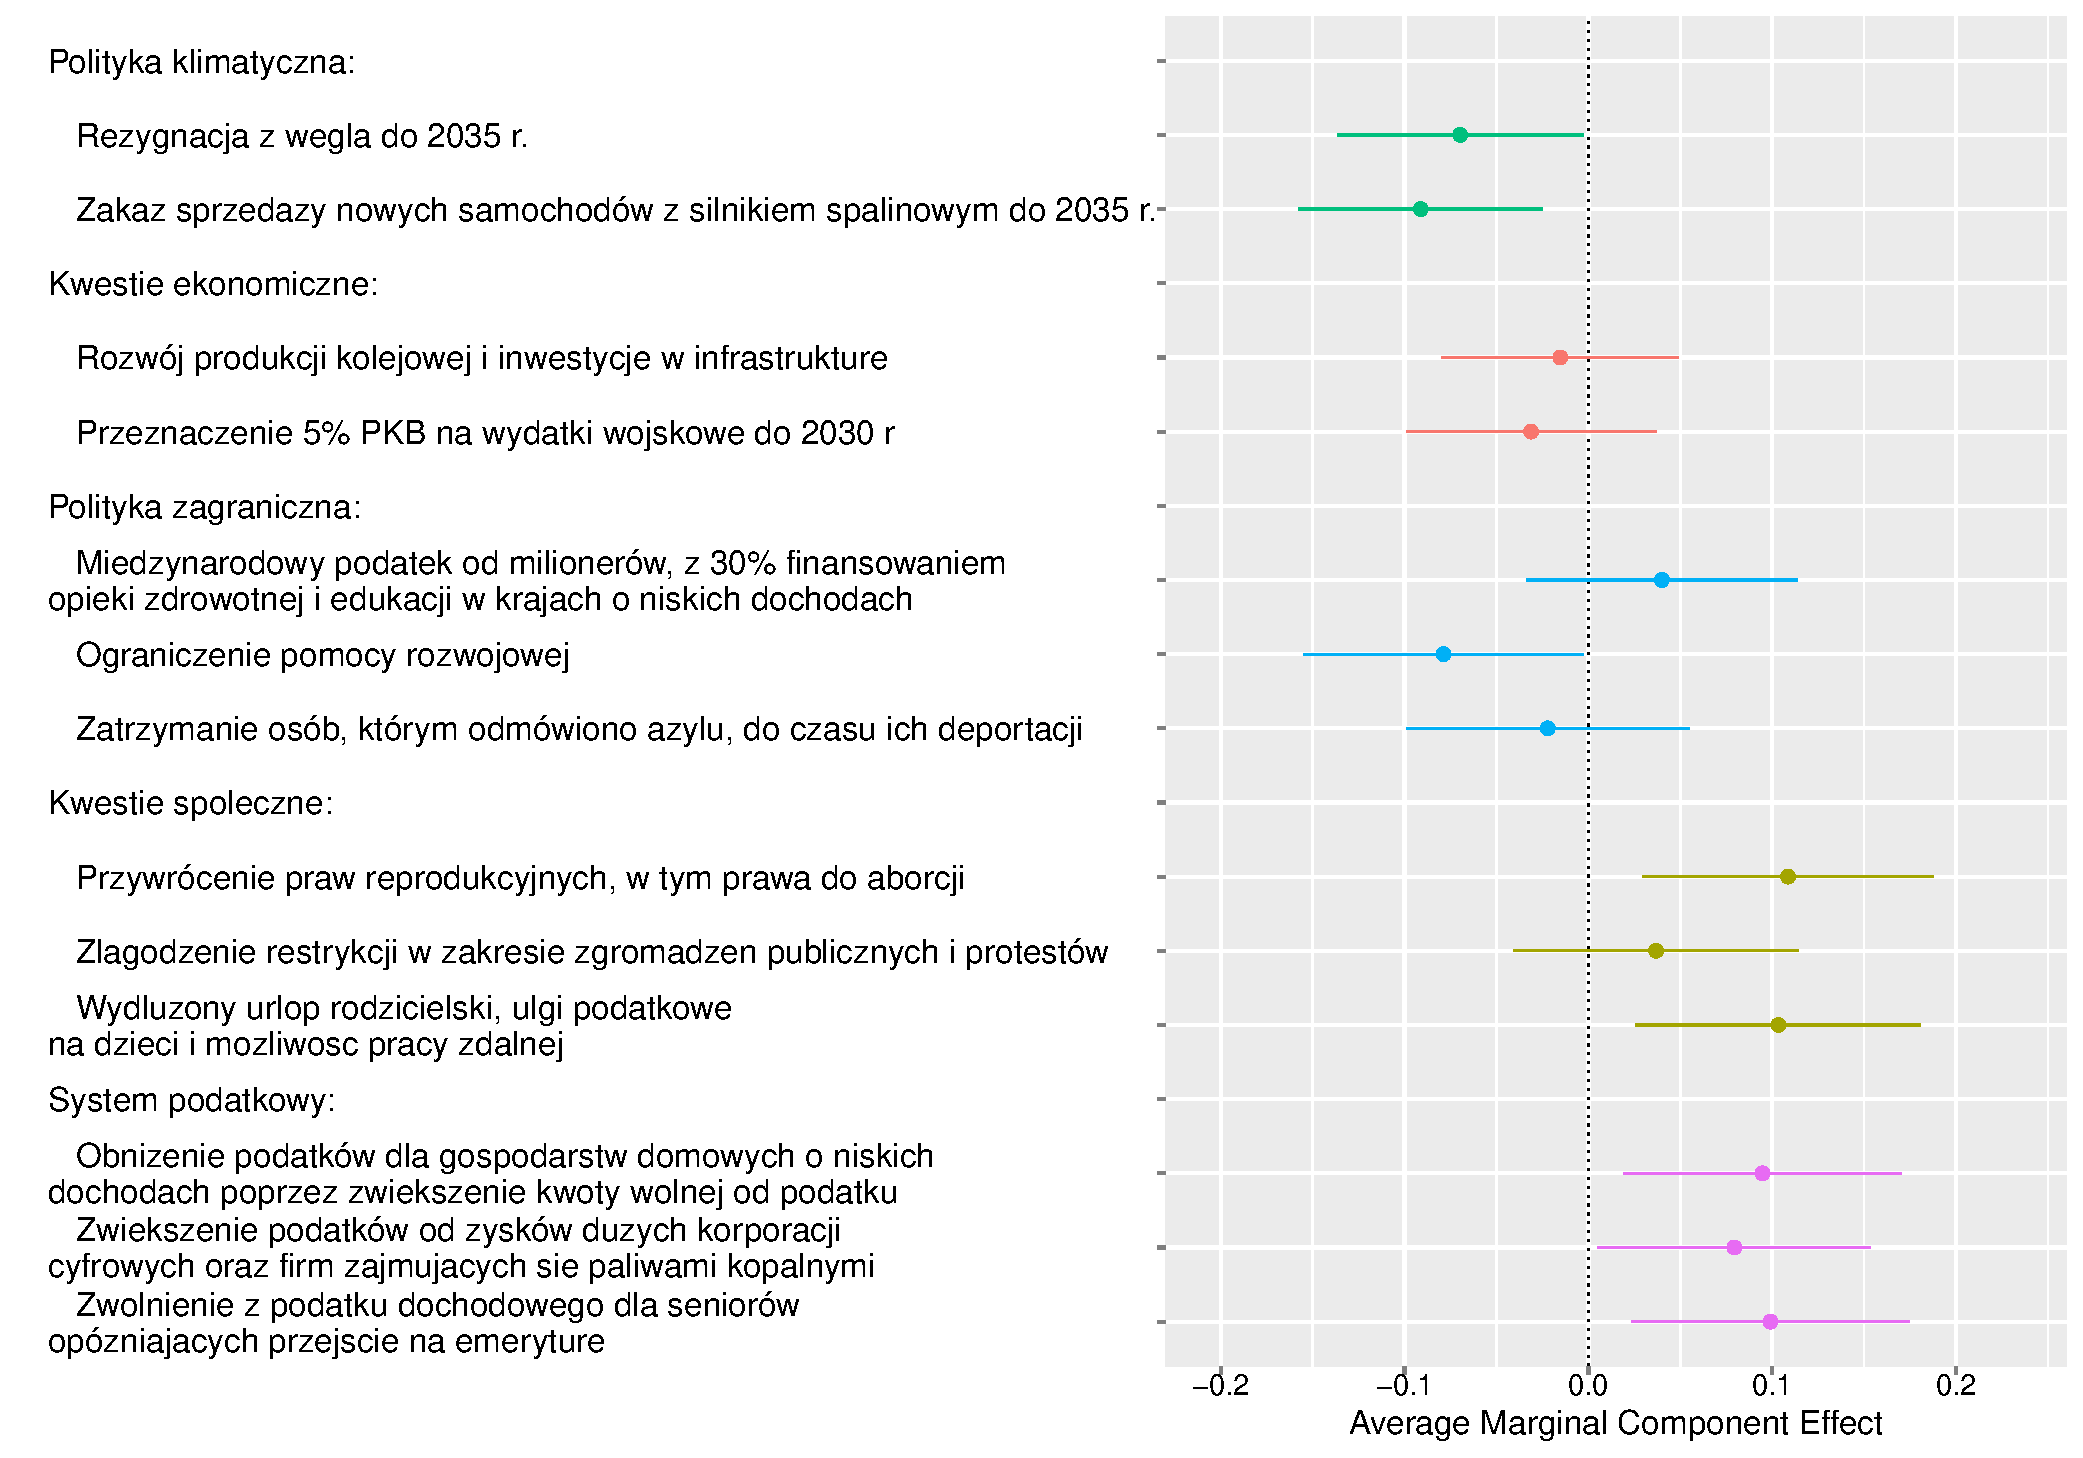
\includegraphics[width=\textwidth]{../figures/all/conjoint_PL.pdf}} 
% \end{figure}

% \begin{figure}[h!]
%     \caption[Conjoint analysis in Spain (Spanish)]{Conjoint analysis in Spain (in Spanish, cf. Figure \ref{fig:conjoint_ES} for English). (Question~\ref{q:conjoint}). \hfill (Back~to~Section~\ref{subsec:conjoint}.)
%     }\label{fig:conjoint_ES_original}
%     \makebox[\textwidth][c]{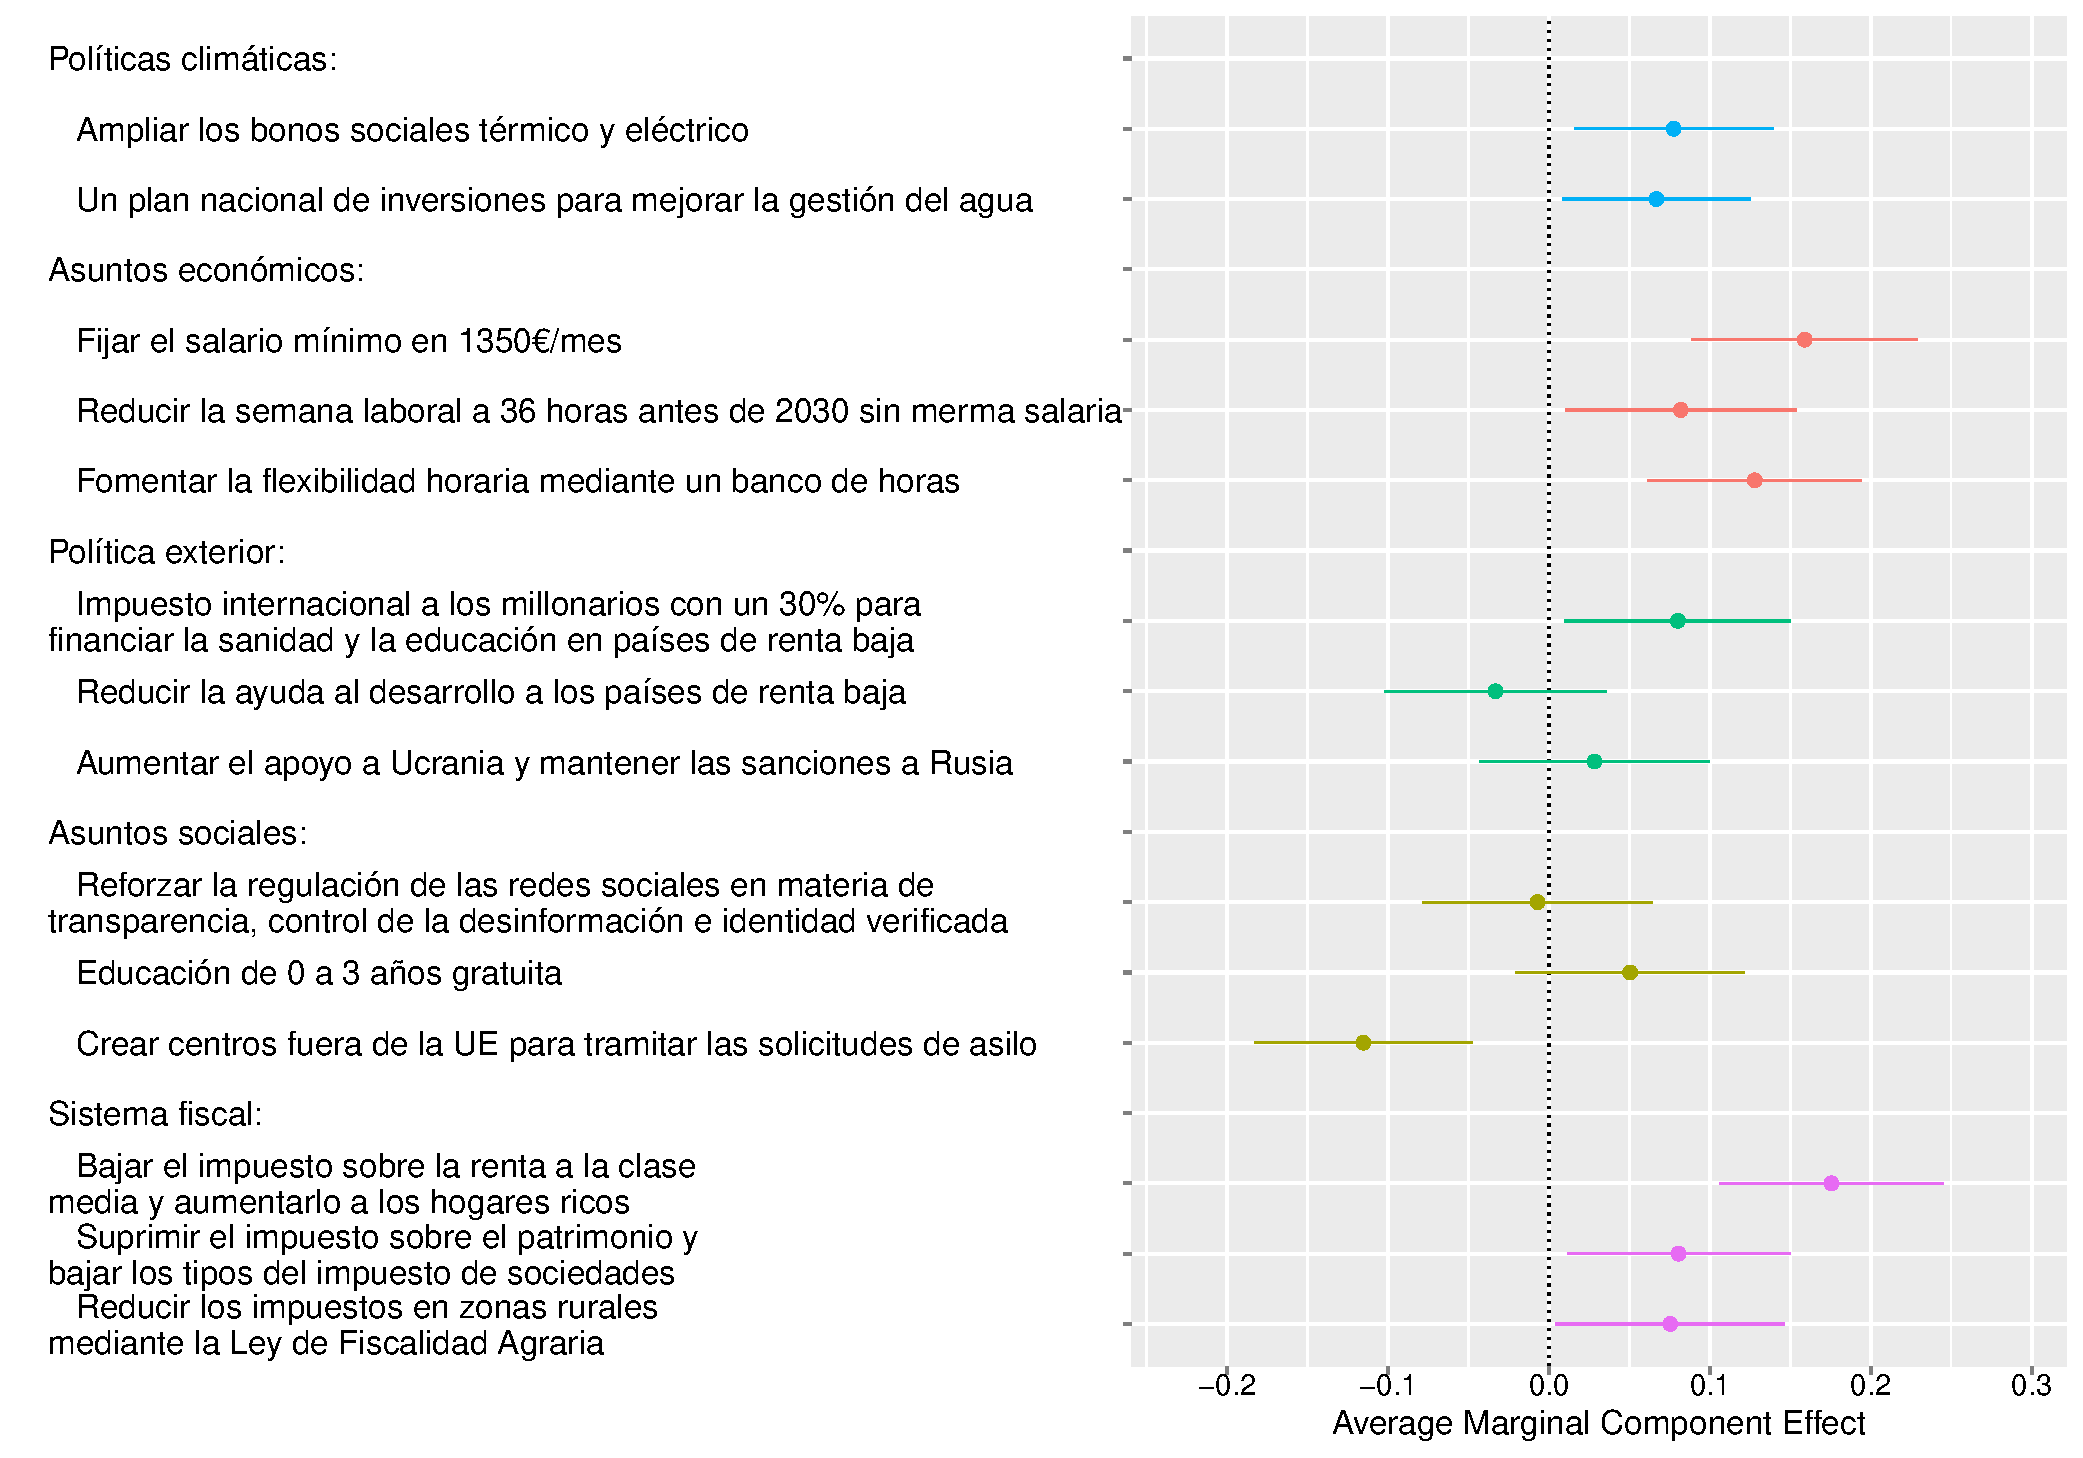
\includegraphics[width=\textwidth]{../figures/all/conjoint_ES-ES.pdf}} 
% \end{figure}

% \begin{figure}[h!]
%     \caption[Conjoint analysis in Japan (Japanese)]{Conjoint analysis in Japan (in Japanese, cf. Figure \ref{fig:conjoint_JP} for English). (Question~\ref{q:conjoint}). \hfill (Back~to~Section~\ref{subsec:conjoint}.)
%     }\label{fig:conjoint_JP_original}
%     \makebox[\textwidth][c]{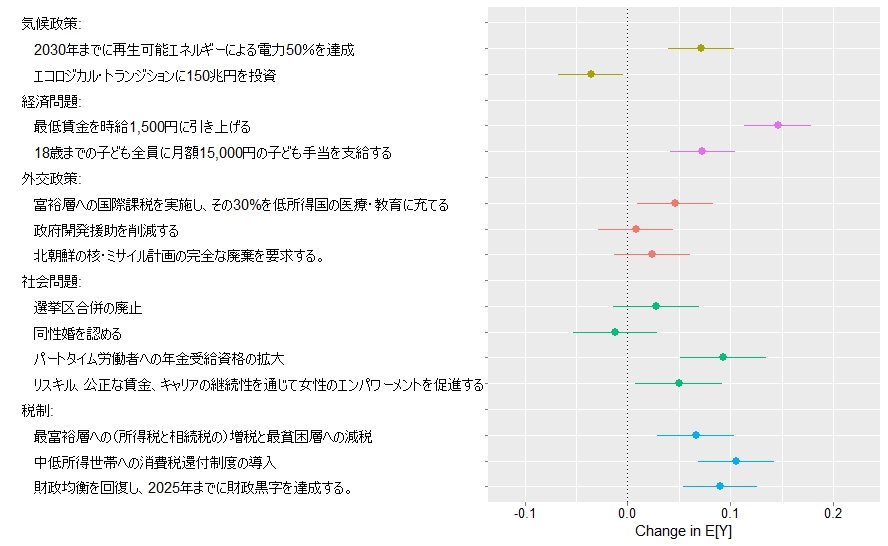
\includegraphics[width=\textwidth]{../figures/JP/conjoint_JA.png}} 
% \end{figure}

\begin{figure}[h!]
    \caption[Average preferred revenue split (\textit{few})]{Average preferred revenue split for a global wealth tax (variant \textit{few}). (Question~\ref{q:revenue_split_few}). \hfill (Back~to~Section~\ref{subsec:revenue_split}.)
    }\label{fig:split_few_bars_nb0}
    \makebox[\textwidth][c]{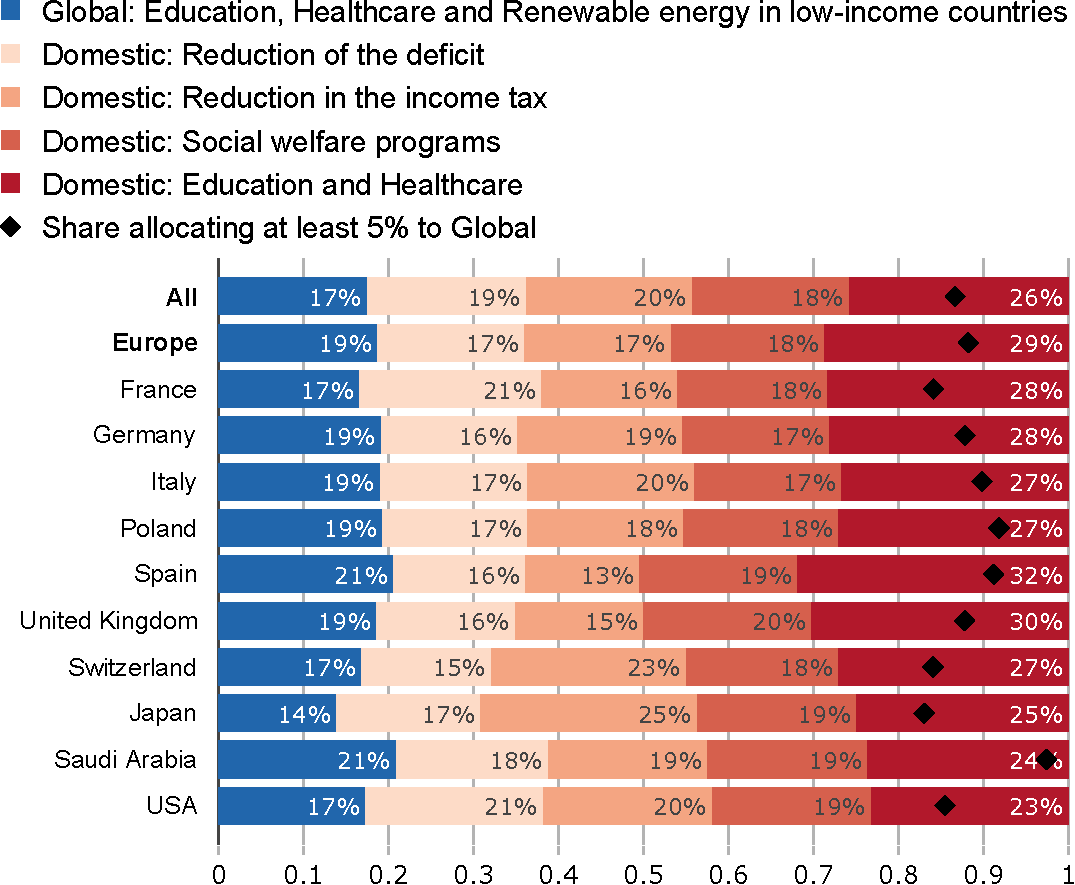
\includegraphics[width=.8\textwidth]{../figures/country_comparison/split_few_bars_nb0.pdf}} 
\end{figure}

\begin{figure}[h!]
    \caption[Decomposition of preferred spending in revenue split, variant \textit{Few}]{Decomposition of preferred shares for each spending item in the revenue split (\textit{All} countries together; variant \textit{few}). (Question~\ref{q:revenue_split_few}). \hfill (Back~to~Section~\ref{subsec:revenue_split}.)
    }\label{fig:split_few}
    \makebox[\textwidth][c]{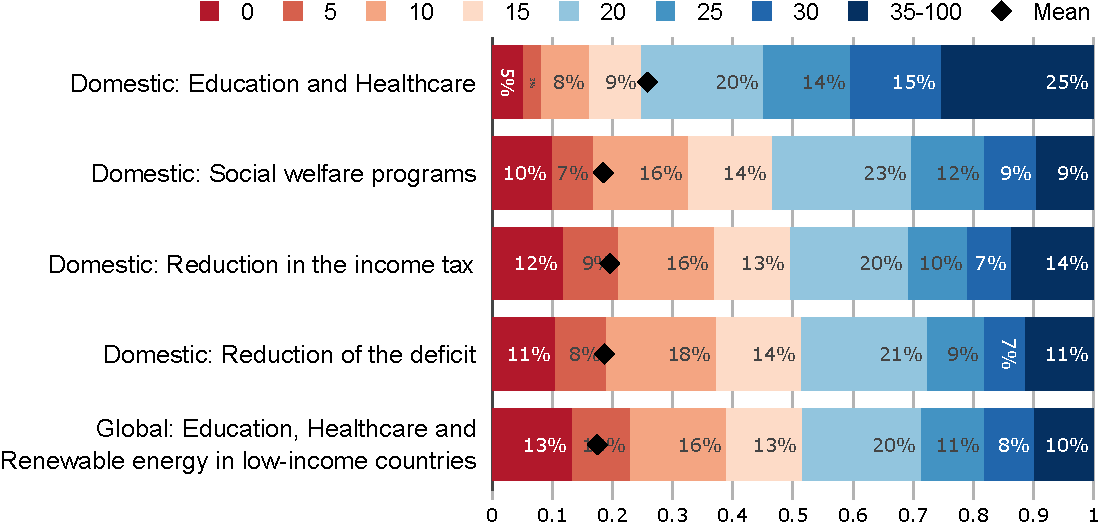
\includegraphics[width=\textwidth]{../figures/all/split_few.pdf}} 
\end{figure}

% \begin{figure}[h!]
%     \caption[Decomposition of preferred spending in revenue split, variant \textit{Many}]{Decomposition of preferred shares for each spending item in the revenue split (\textit{All} countries together; variant \textit{many}). (Question~\ref{q:revenue_split_many}). \hfill (Back~to~Section~\ref{subsec:revenue_split}.)
%     }\label{fig:split_many}
%     \makebox[\textwidth][c]{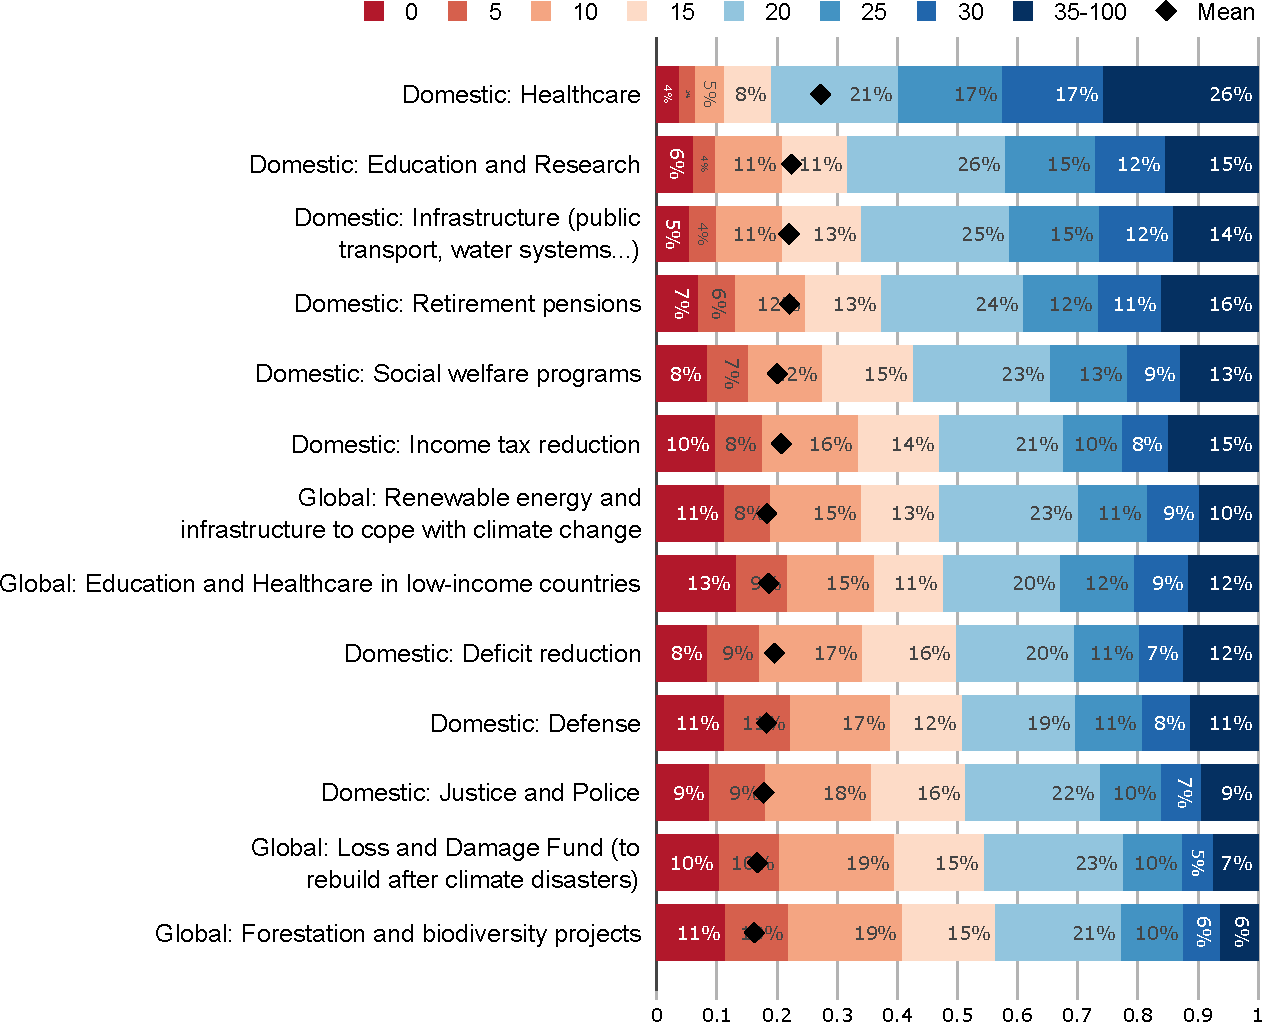
\includegraphics[width=.9\textwidth]{../figures/all/split_many.pdf}} 
% \end{figure}

\begin{figure}[h!]
    \caption[Average preferred revenue split (\textit{many})]{Average preferred revenue split for a global wealth tax (variant \textit{many}). (Question~\ref{q:revenue_split_many}). \hfill (Back~to~Section~\ref{subsec:revenue_split}.)
    }\label{fig:split_many_global_mean}
    \makebox[\textwidth][c]{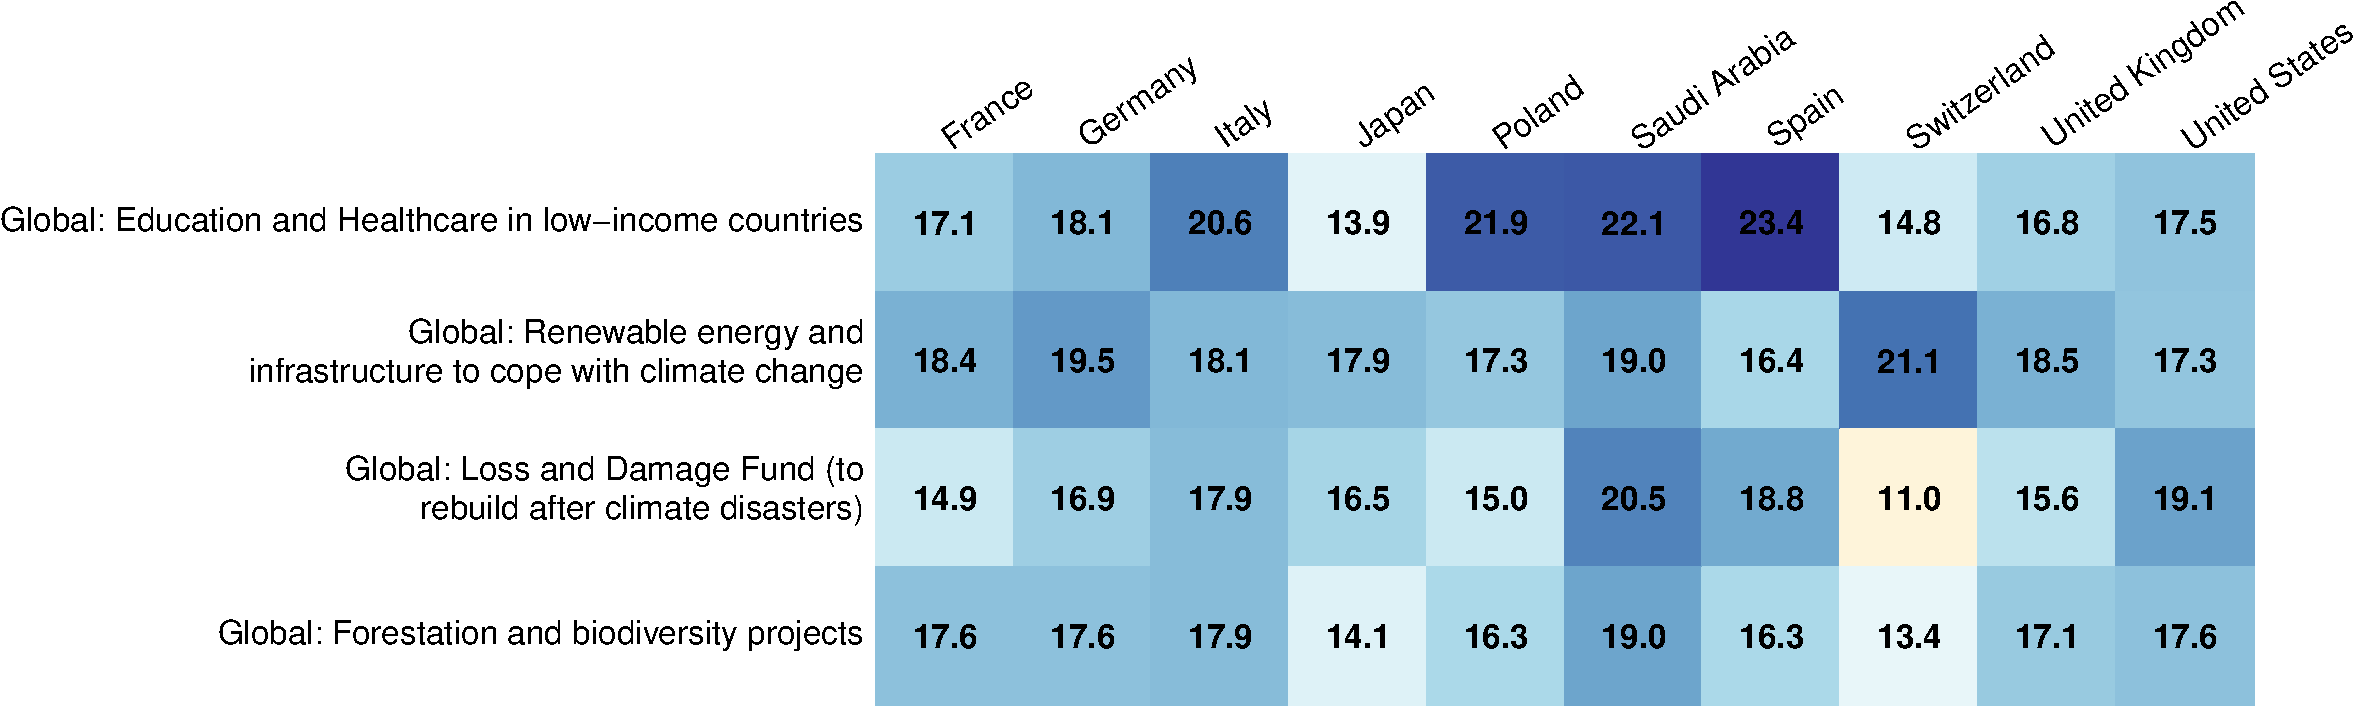
\includegraphics[width=\textwidth]{../figures/country_comparison/split_many_global_mean.pdf}} 
\end{figure} 

% % \begin{figure}[h!]
% %     \caption[]{. (Question~\ref{q:gcs_support}).
% %     }\label{fig:gcs_support}
% %     \makebox[\textwidth][c]{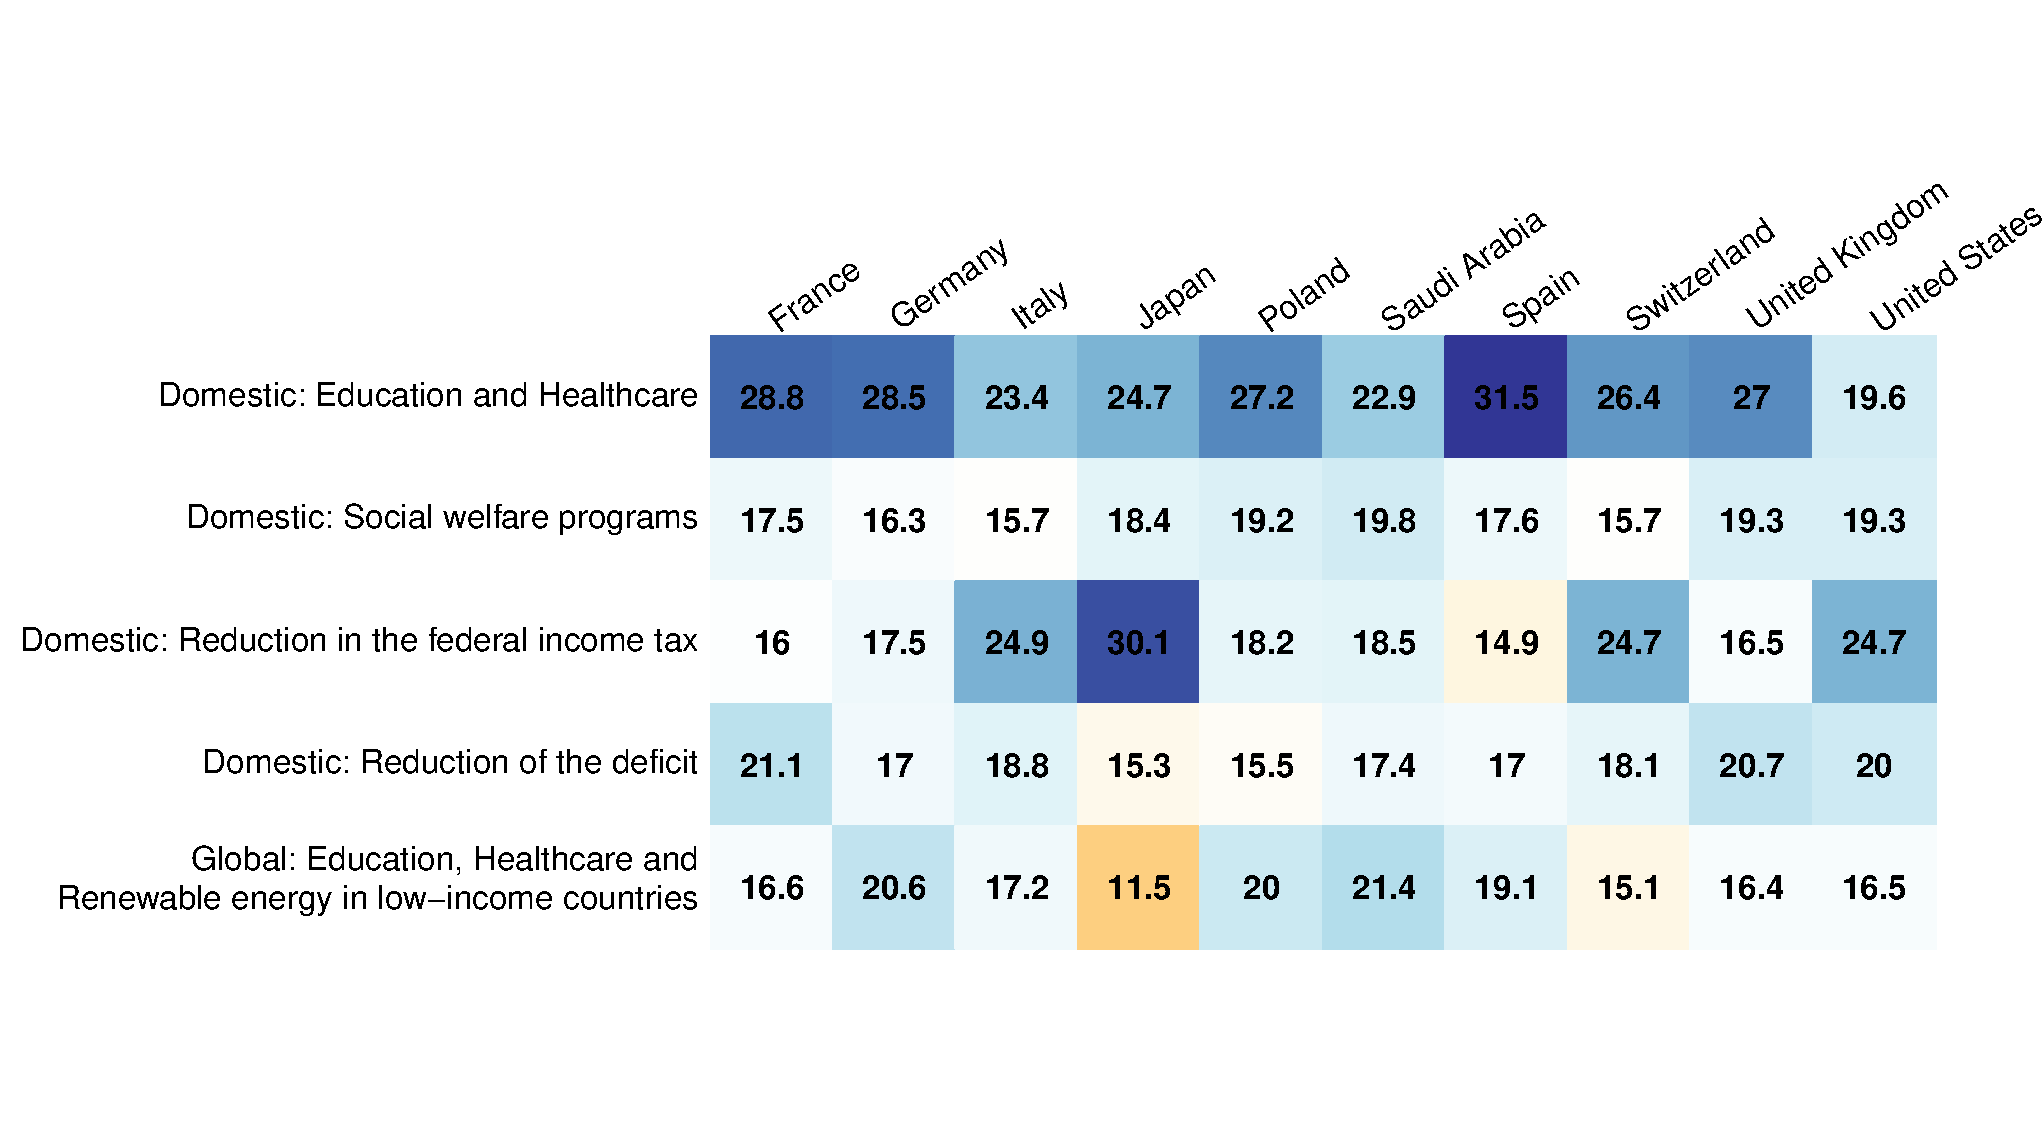
\includegraphics[width=\textwidth]{../figures/country_comparison/split_few_mean.pdf}} 
% % \end{figure}

% \begin{figure}[h!]
%     \caption[Amounts donated to plant trees.]{``By taking this survey, you will be automatically entered into a lottery to win up to [amount\_lottery: \$100]. \\Should you be selected in the lottery, you will have the option to channel a part of this additional compensation to the charity \textit{Just One Tree} to plant trees.\\\\\textbf{In case you win the lottery, what share of the [amount\_lottery: \$100 prize] would you donate to plant trees?}'' (Question~\ref{q:donation}).
%     }\label{fig:donation}
%     \makebox[\textwidth][c]{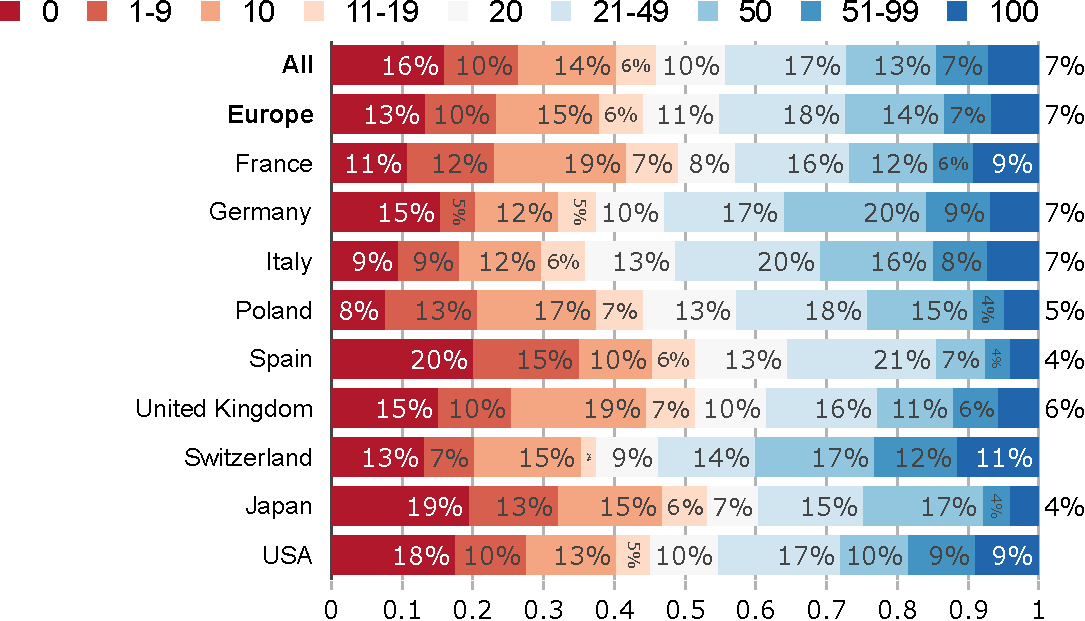
\includegraphics[width=.8\textwidth]{../figures/country_comparison/donation_agg_nolabel.pdf}} 
% \end{figure}

% % \begin{figure}[h!]
% %     \caption[Support for the GCS and belief of support]{Support for the Global Climate Scheme and average belief regarding the support. (Questions~\ref{q:gcs_support}-\ref{q:gcs_belief_own}).
% %     }\label{fig:gcs_belief}
% %     \makebox[\textwidth][c]{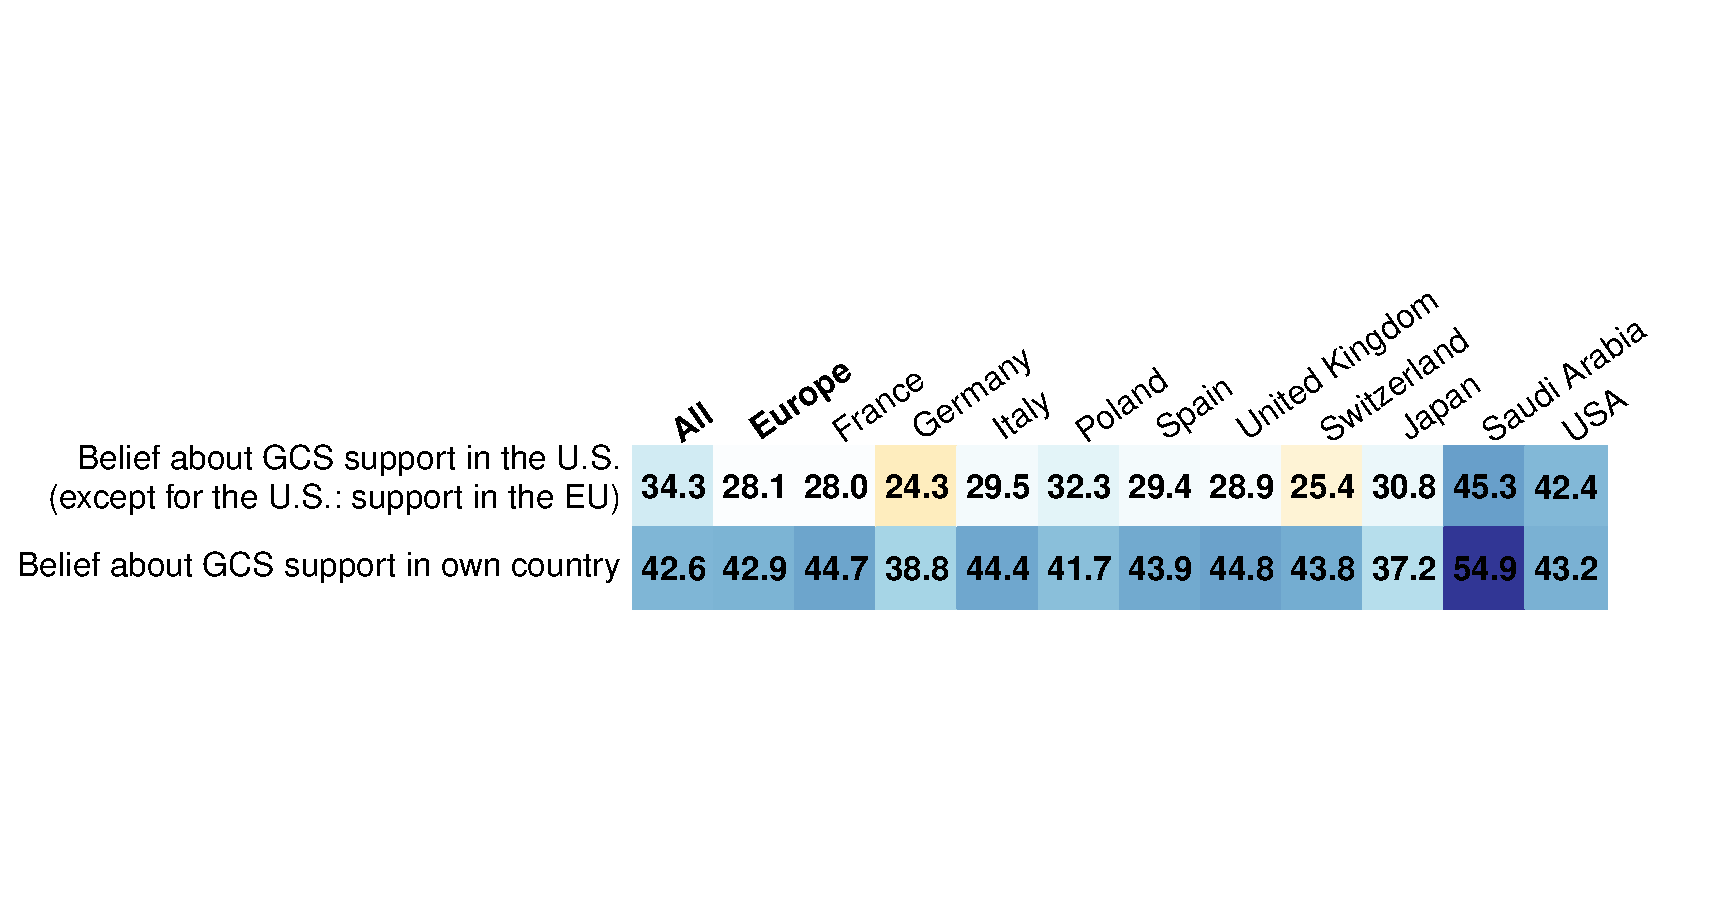
\includegraphics[width=\textwidth]{../figures/country_comparison/gcs_belief_mean.pdf}} 
% % \end{figure} 

\begin{figure}[h!]
    \caption[Support for the NCS, GCS, ICS, and belief of support for GCS]{Support for the National, Global, and International Climate Schemes, and median belief regarding the support for the GCS. (Questions~\ref{q:ncs_support}-\ref{q:ics_support}). \hfill (Back~to~Section~\ref{subsec:ics}.)
    }\label{fig:ncs_gcs_ics}
    \makebox[\textwidth][c]{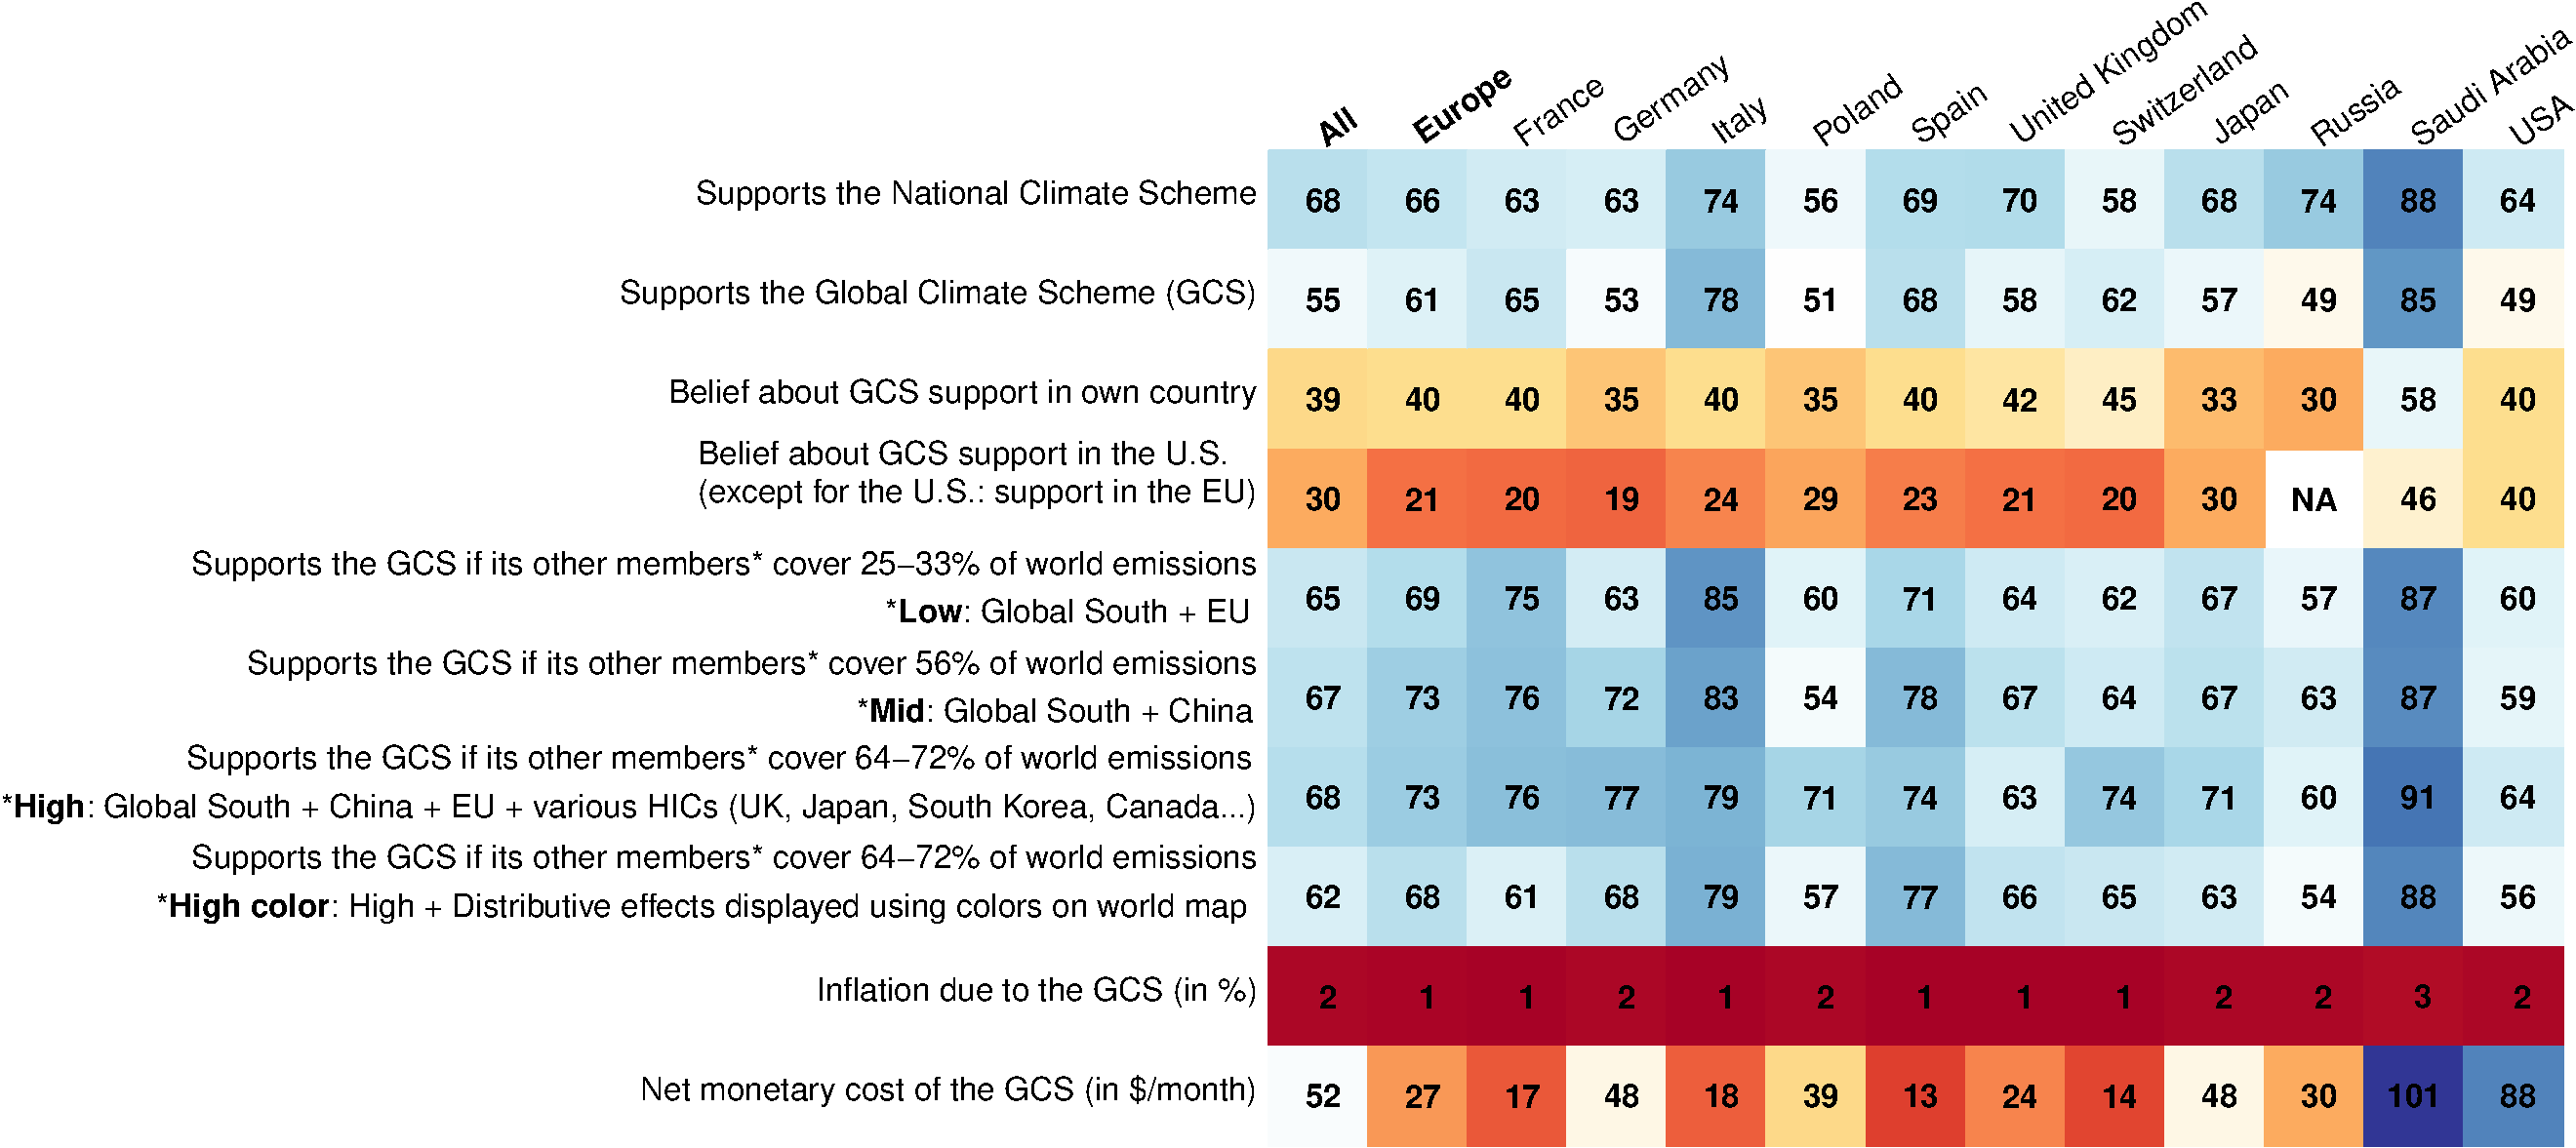
\includegraphics[width=\textwidth]{../figures/country_comparison/ncs_gcs_ics_all_control_features_median_belief_various.pdf}} % ncs_gcs_ics_all_control_median_belief_various?
\end{figure} 
% % TODO? CDF belief?

% \begin{figure}[h!]
%     \caption[Belief about the likelihood of global redistribution]{``According to you, how likely is it that international policies involving significant transfers from high-income countries to low-income countries will be introduced in the next 15 years?'' (Question~\ref{q:likely_solidarity}).
%     }\label{fig:likely_solidarity}
%     \makebox[\textwidth][c]{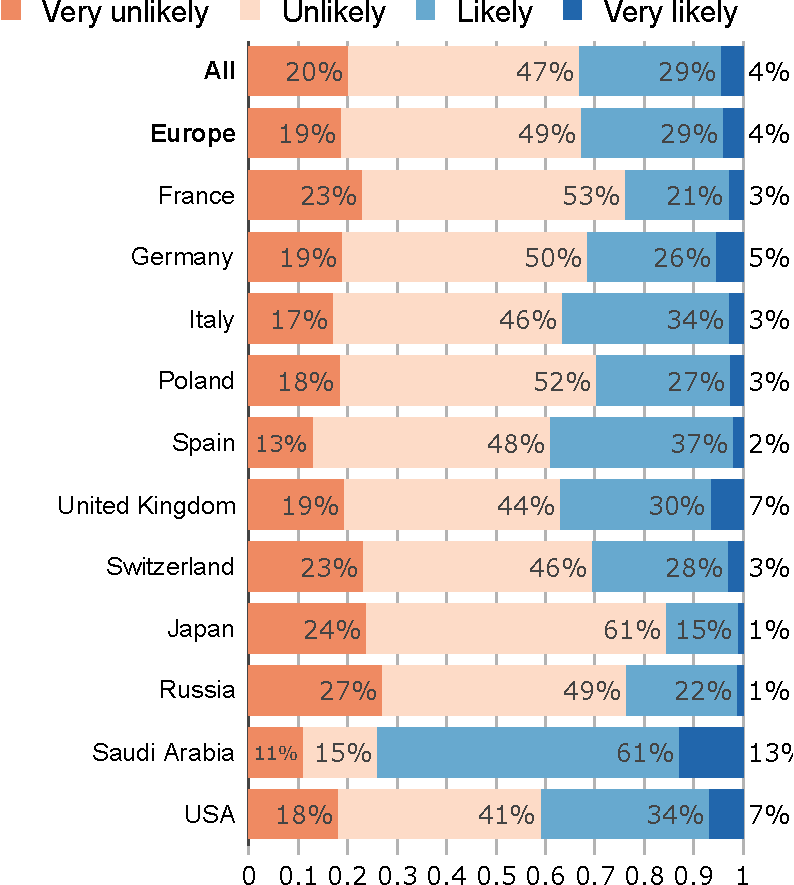
\includegraphics[width=.7\textwidth]{../figures/country_comparison/likely_solidarity_nolabel.pdf}} 
% \end{figure}

\begin{figure}[h!]
    \caption[Absolute support for plausible global redistribution policies]{Absolute support for plausible global redistribution policies (Percentage of \textit{Somewhat} or \textit{Strongly support}). See Figure~\ref{fig:solidarity_support_share} for the relative support. (Question~\ref{q:solidarity_support}).
    }\label{fig:solidarity_support_positive}
    \makebox[\textwidth][c]{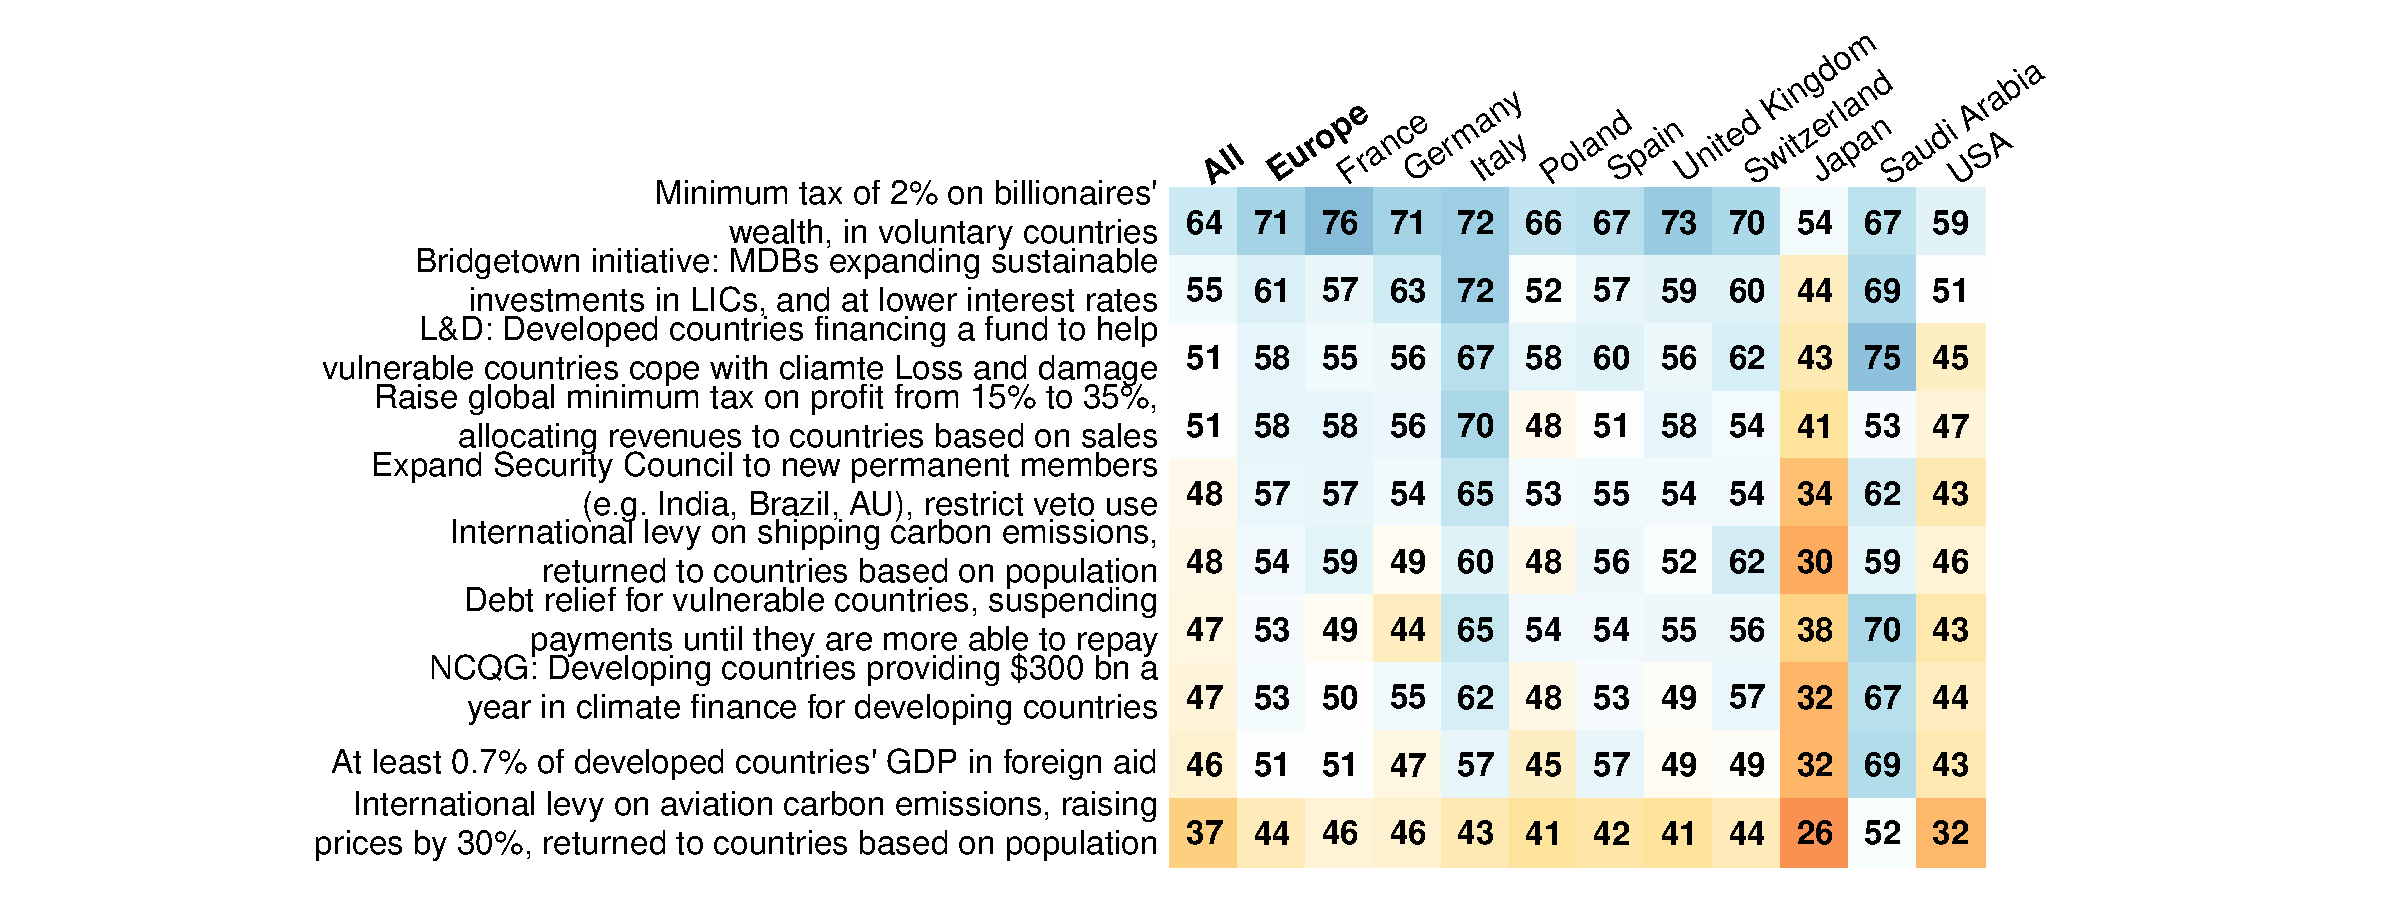
\includegraphics[width=\textwidth]{../figures/country_comparison/solidarity_support_positive.pdf}} 
\end{figure}

% % \begin{figure}[h!]
% %     \caption[Average synthetic indicators of support for global redistribution]{Average synthetic indicators of support for global redistribution. (Question~\ref{q:solidarity_support}). \hfill (Back~to~Section~\ref{par:ranking}.)
% %     }\label{fig:synthetic_indicators_mean}
% %     \makebox[\textwidth][c]{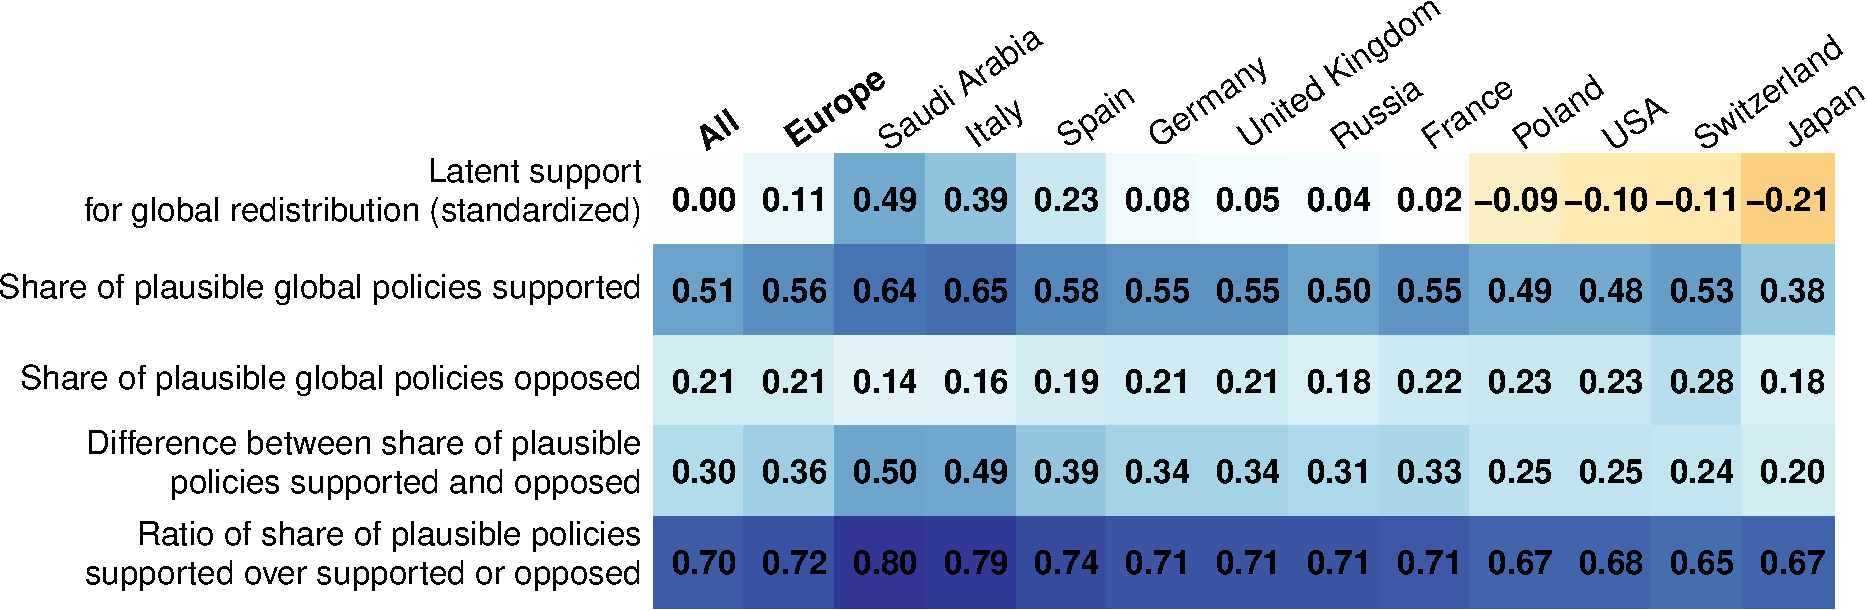
\includegraphics[width=\textwidth]{../figures/country_comparison/synthetic_indicators_mean.pdf}} 
% % \end{figure}


% \begin{figure}[h!]
%     \caption[Share of plausible global policies supported]{Share of plausible global redistribution policies supported (\textit{somewhat} or \textit{strongly}). (Question~\ref{q:solidarity_support}). \hfill Section~\ref{subsec:debated}.
%     }\label{fig:share_solidarity_supported}
%     \makebox[\textwidth][c]{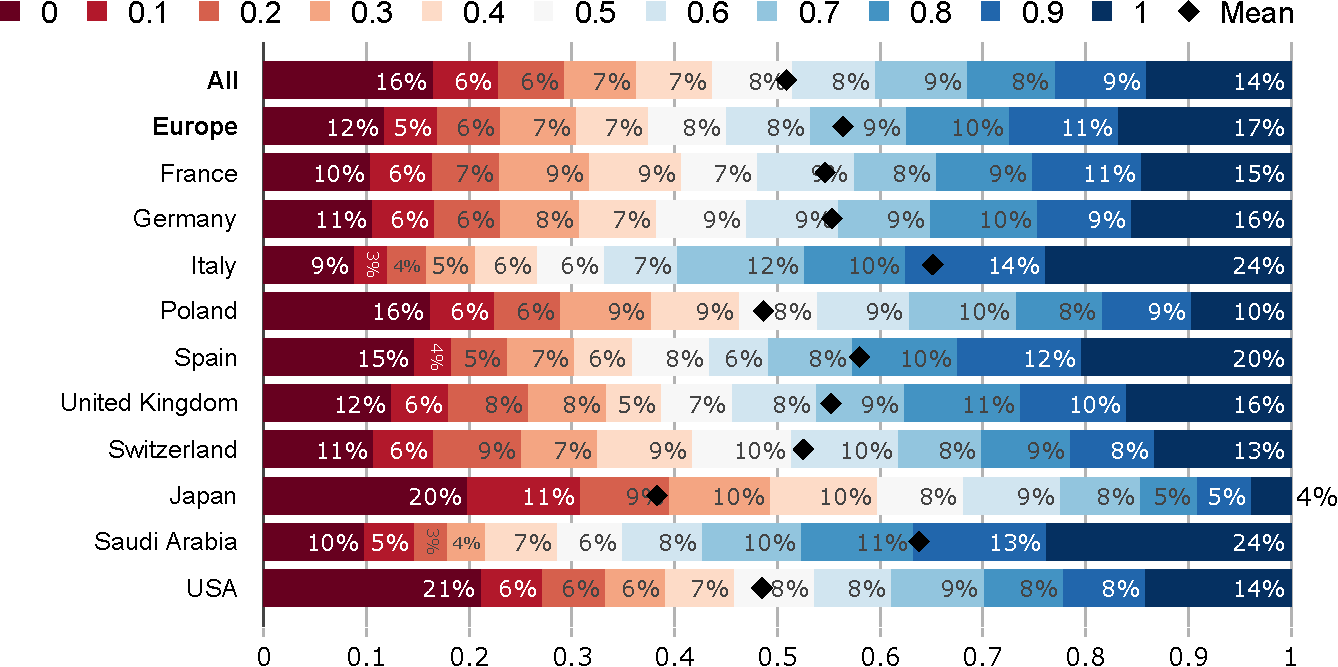
\includegraphics[width=\textwidth]{../figures/country_comparison/share_solidarity_supported_nolabel.pdf}} 
% \end{figure}

% \begin{figure}[h!]
%     \caption[Share of plausible global policies opposed]{Share of plausible global redistribution policies opposed (\textit{somewhat} or \textit{strongly}). (Question~\ref{q:solidarity_support}). \hfill Section~\ref{subsec:debated}.
%     }\label{fig:share_solidarity_opposed}
%     \makebox[\textwidth][c]{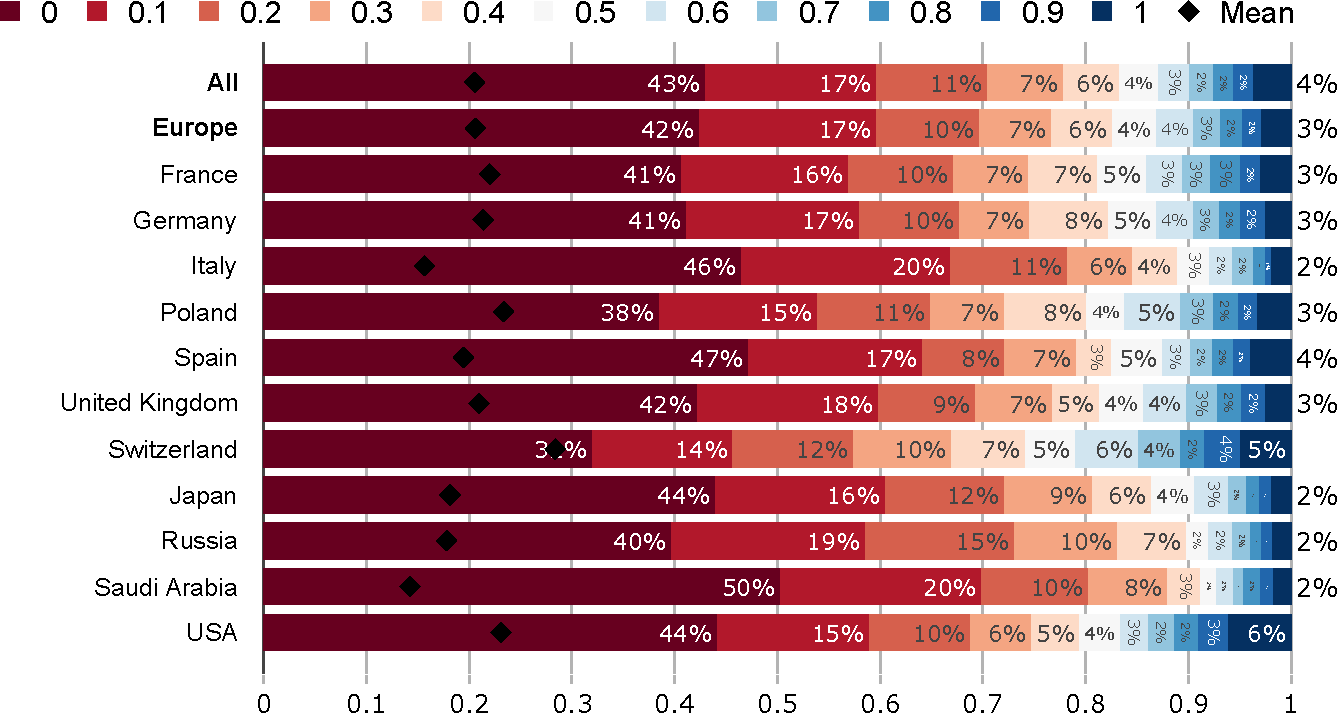
\includegraphics[width=\textwidth]{../figures/country_comparison/share_solidarity_opposed_nolabel.pdf}} 
% \end{figure}

\begin{figure}[h!]
    \caption[Preferred NCQG, variant \textit{Short}]{Preferred North-to-South climate grant funding in 2035, specified in qualitative terms or in terms of who advocates for that amount (NCQG, variant \textit{Short}). (Question~\ref{q:ncqg}). \hfill (Back~to~Section~\ref{par:ncqg}.)
    }\label{fig:ncqg}
    \makebox[\textwidth][c]{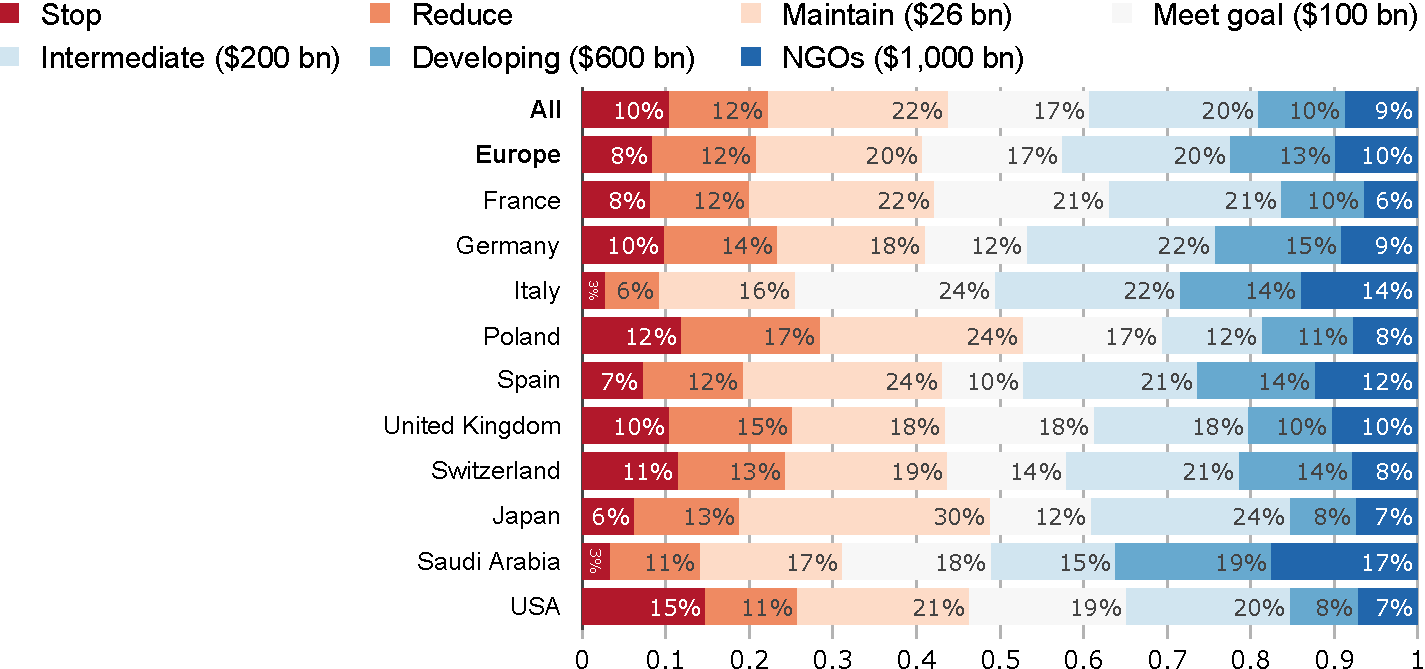
\includegraphics[width=\textwidth]{../figures/country_comparison/ncqg_nolabel.pdf}} 
\end{figure}

\begin{figure}[h!]
    \caption[Preferred NCQG, variant \textit{Full}]{Preferred North-to-South climate grant funding in 2035, specified in money terms (NCQG, variant \textit{Full}). (Question~\ref{q:ncqg_full}). \hfill (Back~to~Section~\ref{par:ncqg}.)
    }\label{fig:ncqg_full}
    \makebox[\textwidth][c]{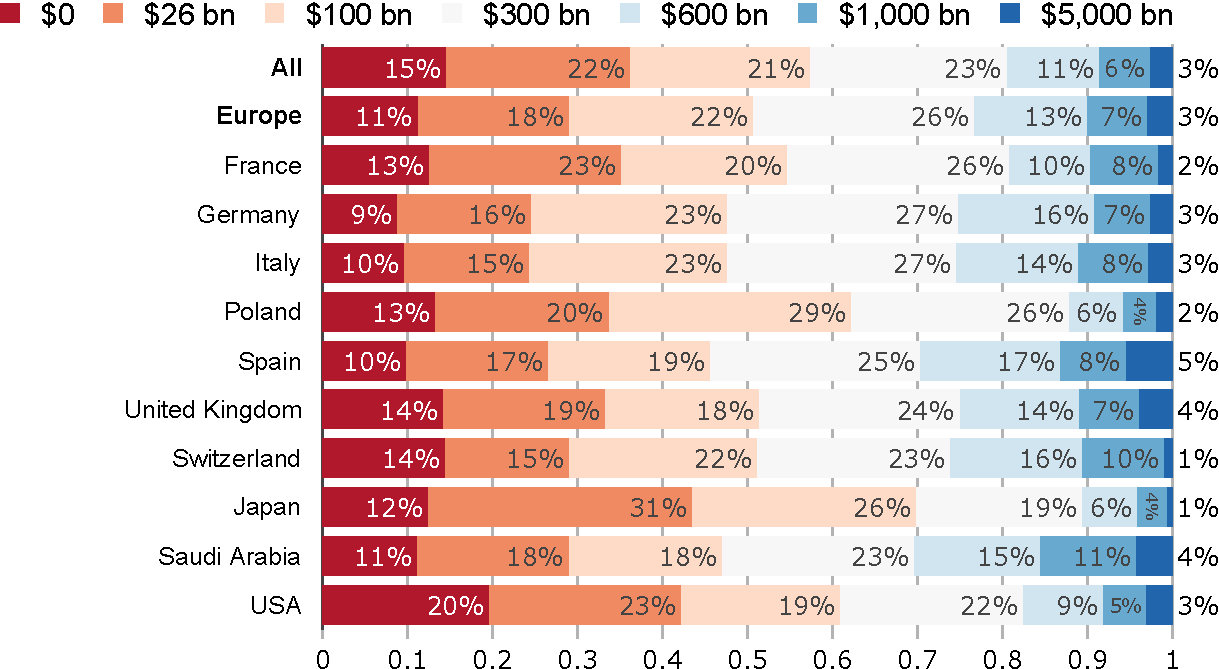
\includegraphics[width=\textwidth]{../figures/country_comparison/ncqg_full_nolabel.pdf}} 
\end{figure}

% \begin{figure}[h!]
%     \caption[Support for an international wealth depending on country coverage]{Support for an international wealth tax with 30\% of revenue funding LICs, depending on the country coverage (\textit{Yes}/\textit{No} question). (Questions~\ref{q:global_tax_support}-\ref{q:intl_tax_support}).
%     }\label{fig:wealth_tax_heatmap}
%     \makebox[\textwidth][c]{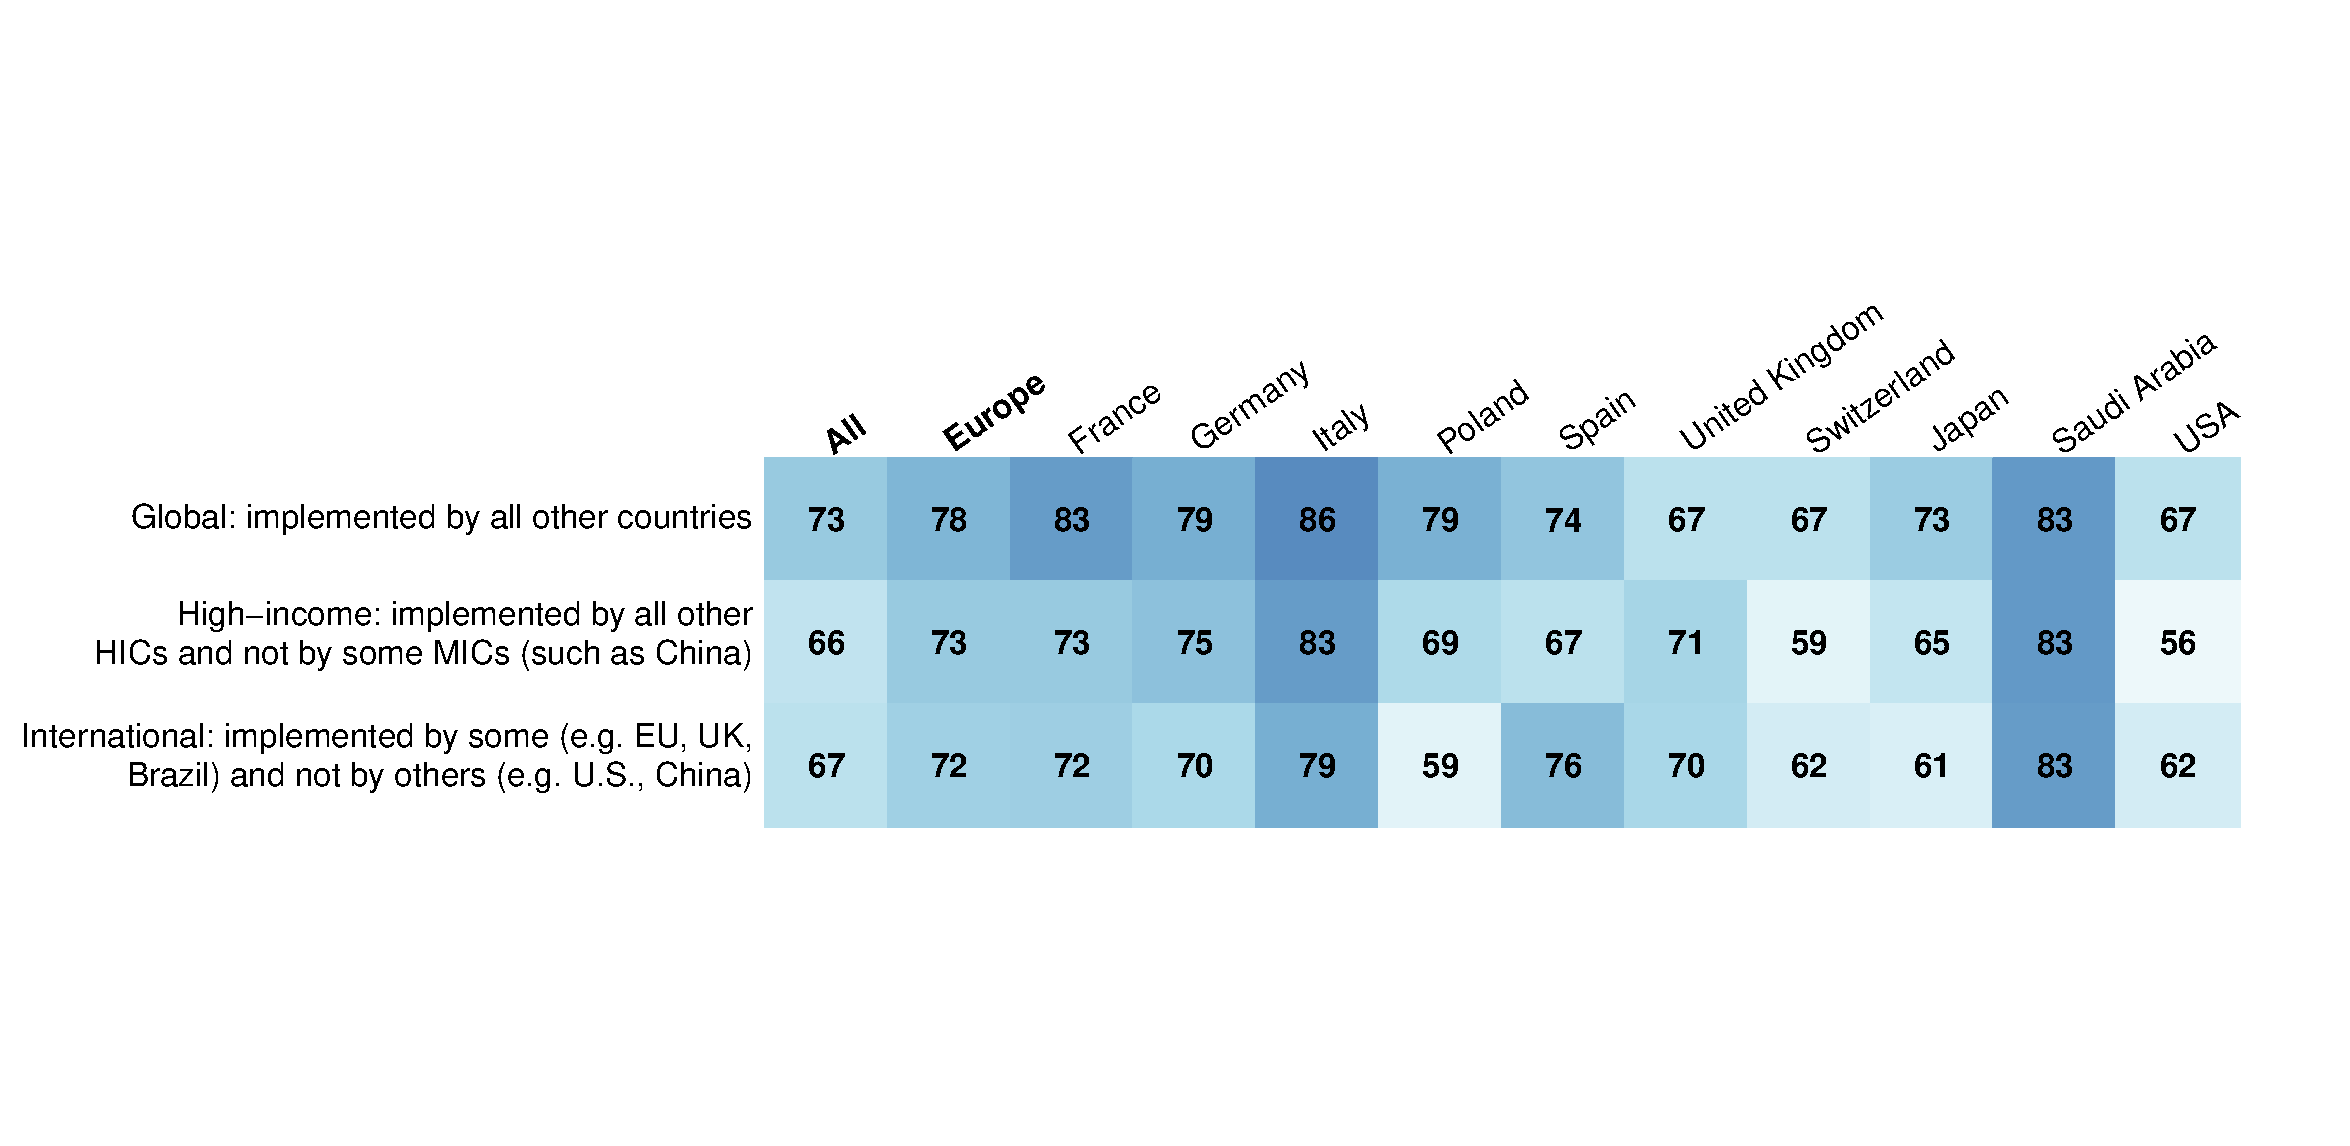
\includegraphics[width=\textwidth]{../figures/country_comparison/wealth_tax_support_positive.pdf}} 
% \end{figure}

% \begin{figure}[h!]
%     \caption[Prefers a sustainable future]{Prefers a \textit{sustainable} rather than a \textit{business-as-usual} future. (Question~\ref{q:sustainable_future}).
%     }\label{fig:sustainable_future}
%     \makebox[\textwidth][c]{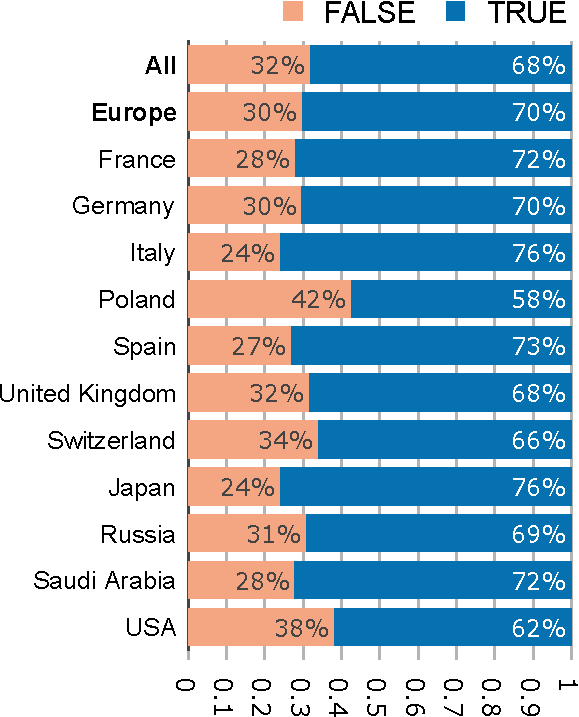
\includegraphics[width=.5\textwidth]{../figures/country_comparison/sustainable_future_nolabel.pdf}} 
% \end{figure}

\begin{figure}[h!]
    \caption[Acceptance of a global income tax on the richest to fund LICs]{Acceptance of a global progressive income tax on the richest households to finance poverty reduction in the Global South (Percentage of \textit{Somewhat} or \textit{Strongly support} among non-\textit{Indifferent} responses). (Questions~\ref{q:top1_tax_support}-\ref{q:top3_tax_support}).
    }\label{fig:top_tax_share}
    \makebox[\textwidth][c]{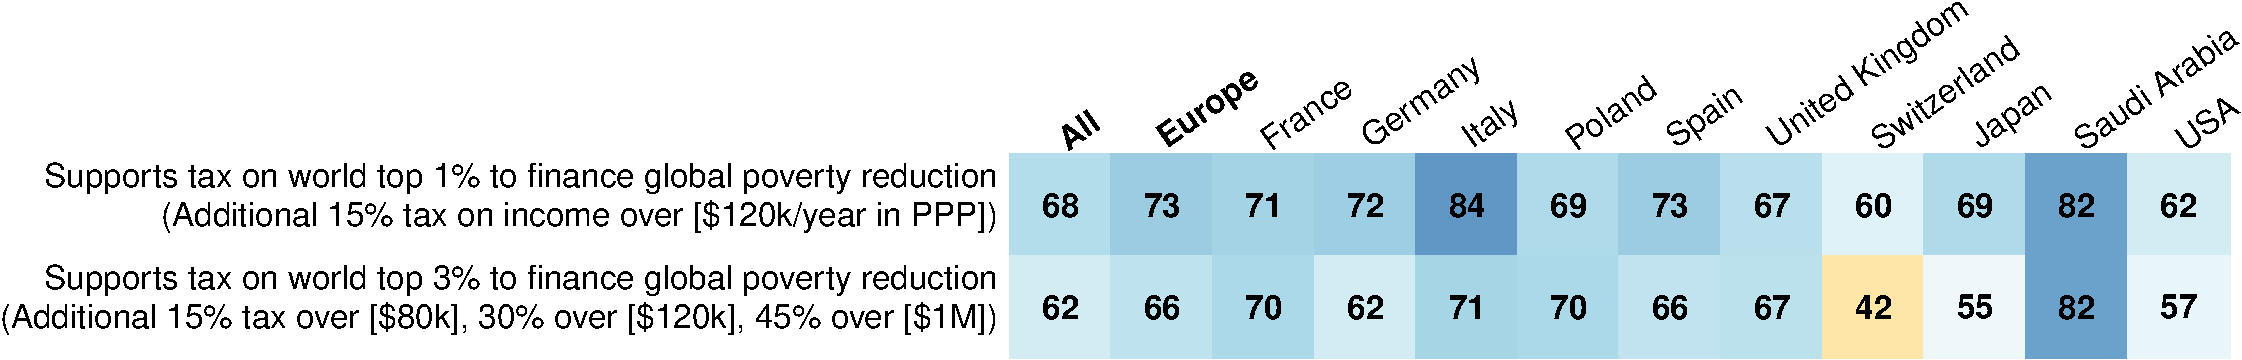
\includegraphics[width=\textwidth]{../figures/country_comparison/top_tax_share.pdf}} 
\end{figure}

\begin{figure}[h!]
    \caption[Acceptance of a global income tax on the richest to fund LICs]{Acceptance of a global progressive income tax on the richest households to finance global poverty reduction (Questions~\ref{q:top1_tax_support}-\ref{q:top3_tax_support}, Percentage of \textit{Somewhat} or \textit{Strongly support} among non-\textit{Indifferent} responses), and features of the tax presented to the respondents (Section~\ref{subsec:country_features}). \hfill (Back~to~Section~\ref{par:global_income_redistr}.)
    }\label{fig:top_tax_share}
    \makebox[\textwidth][c]{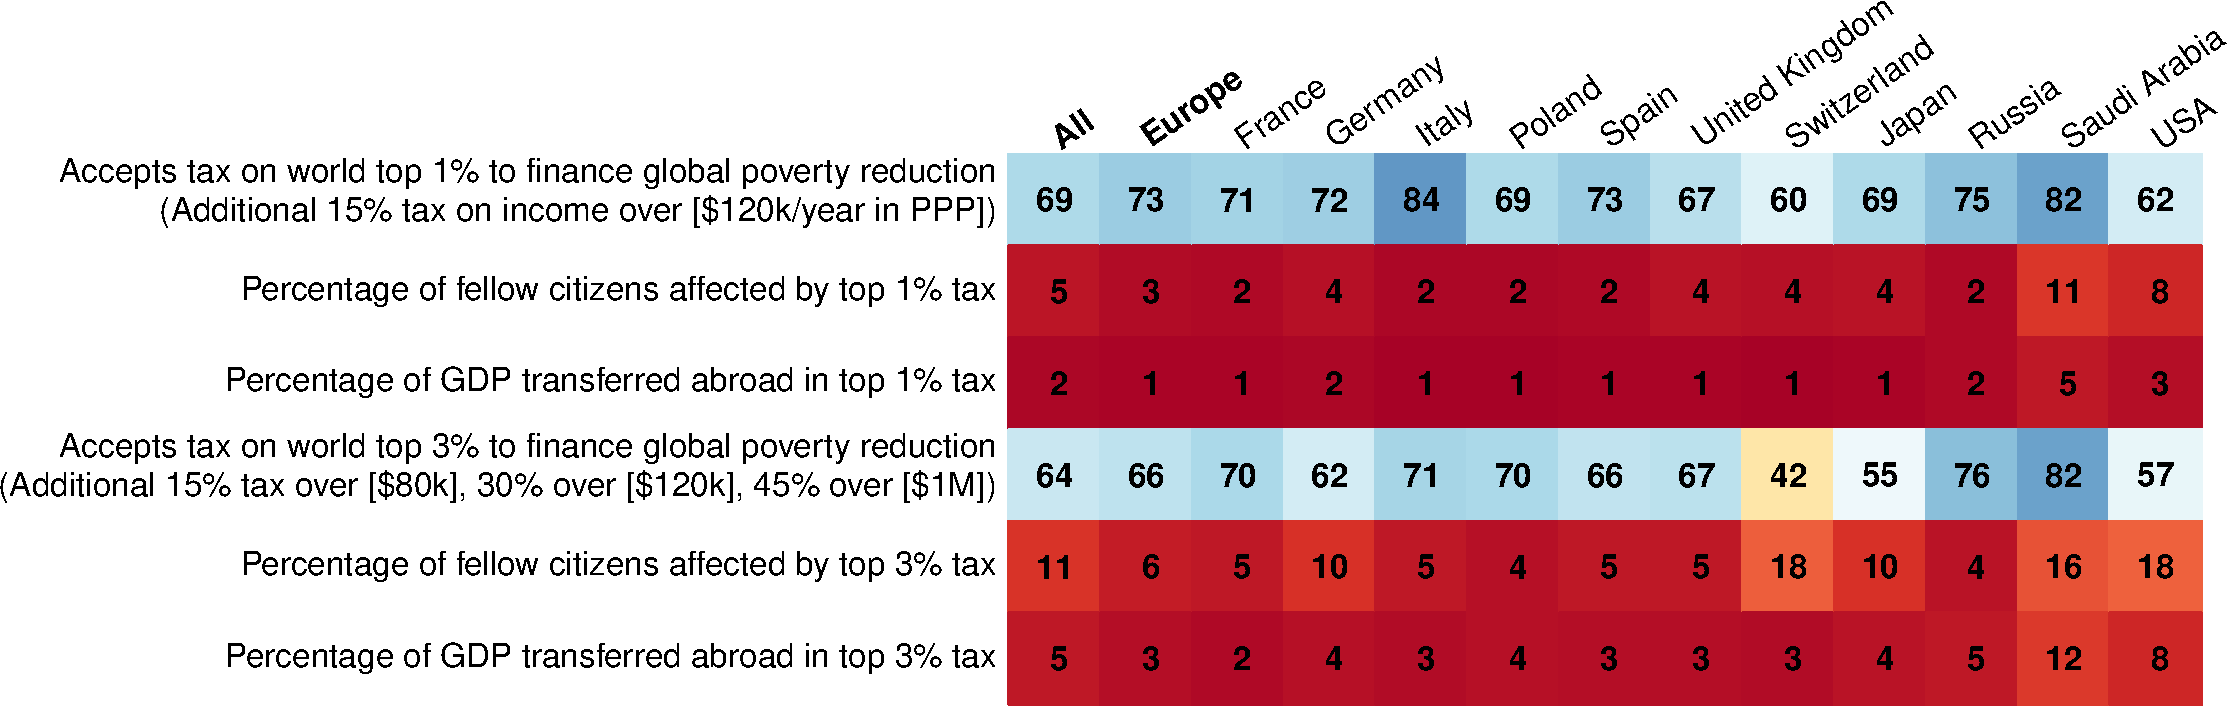
\includegraphics[width=\textwidth]{../figures/country_comparison/top_tax_all_share_various.pdf}} % top_tax_share
\end{figure}

\begin{figure}[h!]
    \caption[Absolute support for an income tax on top 1\% to fund LICs]{Absolute support for a global progressive income tax on the richest households to finance global poverty reduction (Percentage of \textit{Somewhat} or \textit{Strongly support}). (Questions~\ref{q:top1_tax_support}-\ref{q:top3_tax_support}). \hfill (Back~to~Section~\ref{par:global_income_redistr}.)
    }\label{fig:top_tax_positive}
    \makebox[\textwidth][c]{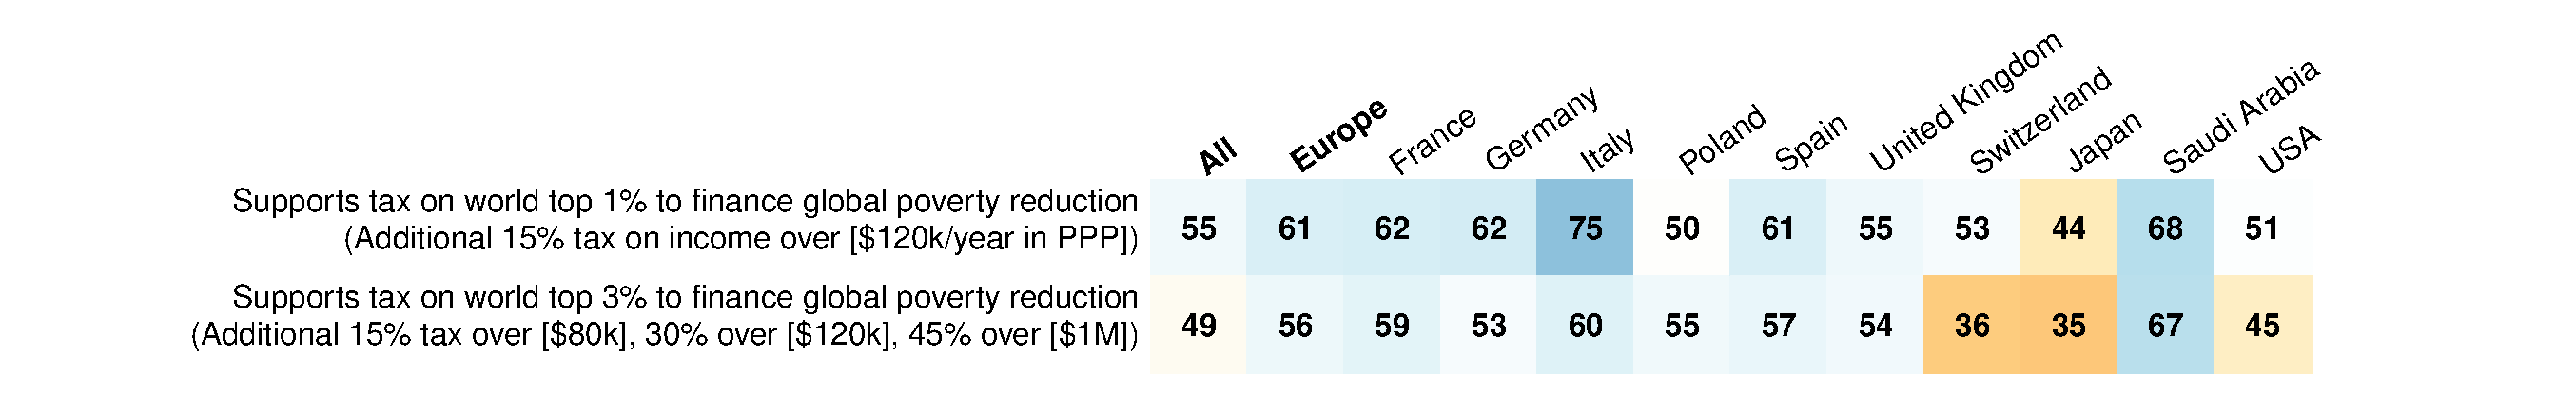
\includegraphics[width=\textwidth]{../figures/country_comparison/top_tax_positive.pdf}} 
\end{figure}

% \begin{figure}[h!]
%     \caption[Acceptance of a global income tax among affected respondents]{Acceptance of a global progressive income tax on the richest households to finance global poverty reduction \textit{among respondents affected by the tax} (Questions~\ref{q:top1_tax_support}-\ref{q:top3_tax_support}, Percentage of \textit{Somewhat} or \textit{Strongly support} among non-\textit{Indifferent} responses), and share of respondents affected by the tax (Section~\ref{subsec:country_features}). \hfill (Back~to~Section~\ref{par:global_income_redistr}.)
%     }\label{fig:top_tax_affected_share}
%     \makebox[\textwidth][c]{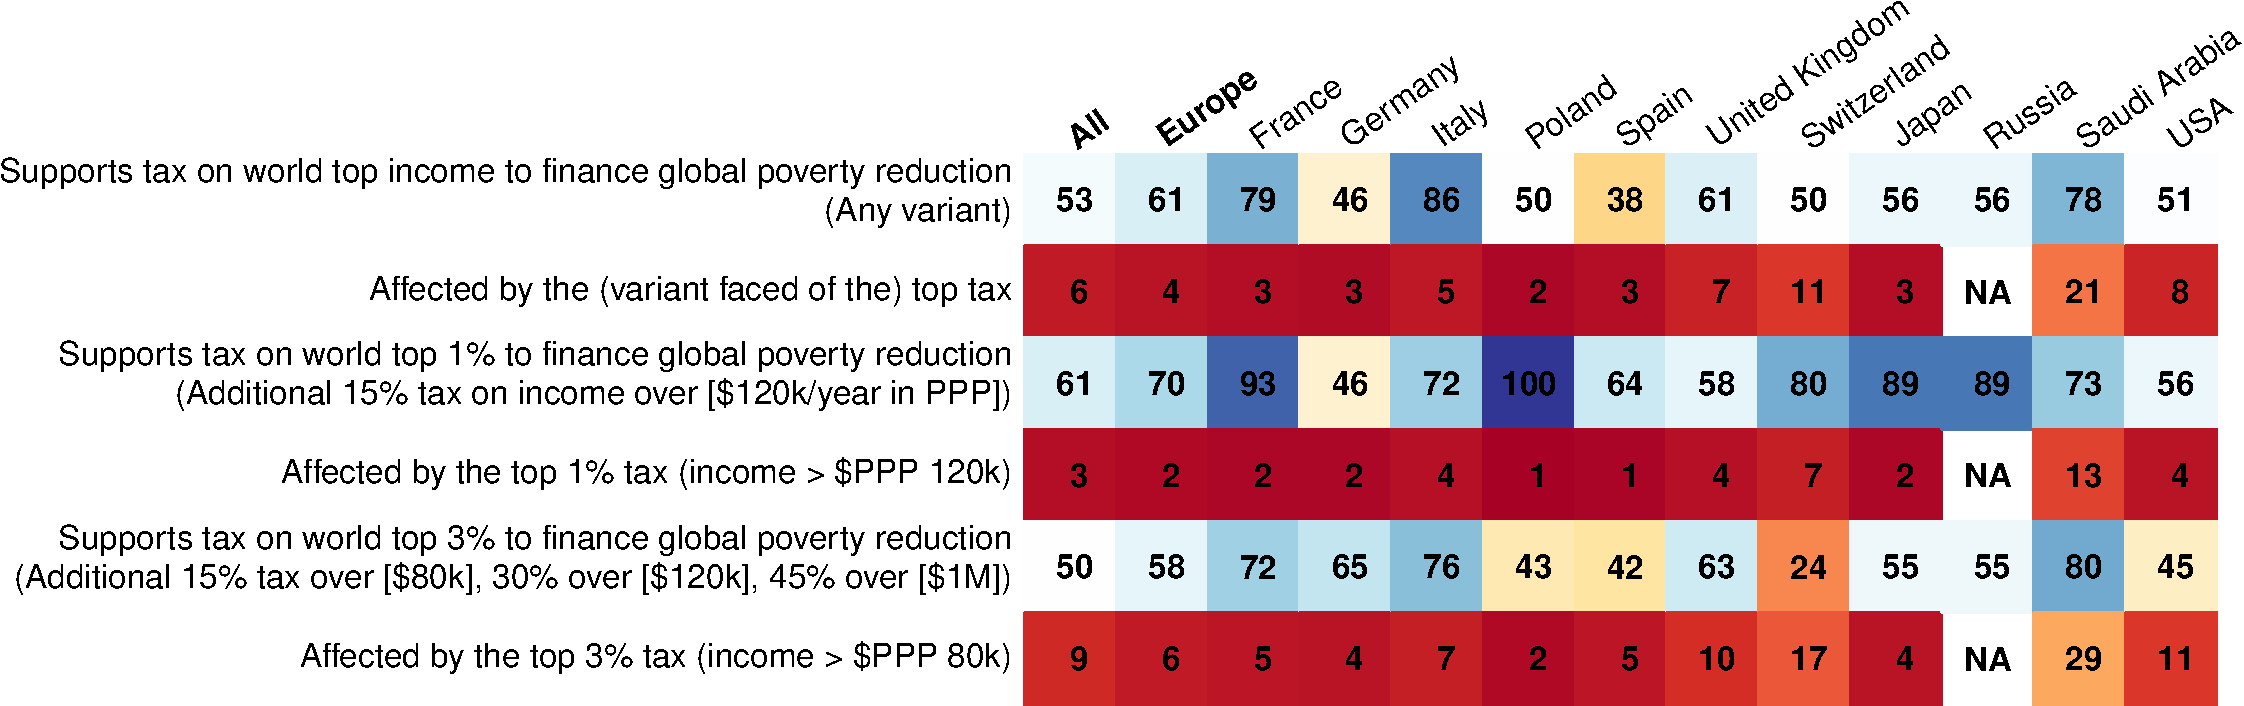
\includegraphics[width=\textwidth]{../figures/country_comparison/top_tax_affected_share_various.pdf}} 
% \end{figure}

% % \begin{figure}[h!]
% %     \caption[\textit{Right} or \textit{Best} way to transfer resources to LICs]{``How do you evaluate each of these channels to transfer resources to reduce poverty in LICs?''\\ Percentage of \textit{Right} or \textit{Best} way (other options: \textit{Wrong} or \textit{Acceptable} way). (Question~\ref{q:transfer_how}).
% %     }\label{fig:transfer_how_positive}
% %     \makebox[\textwidth][c]{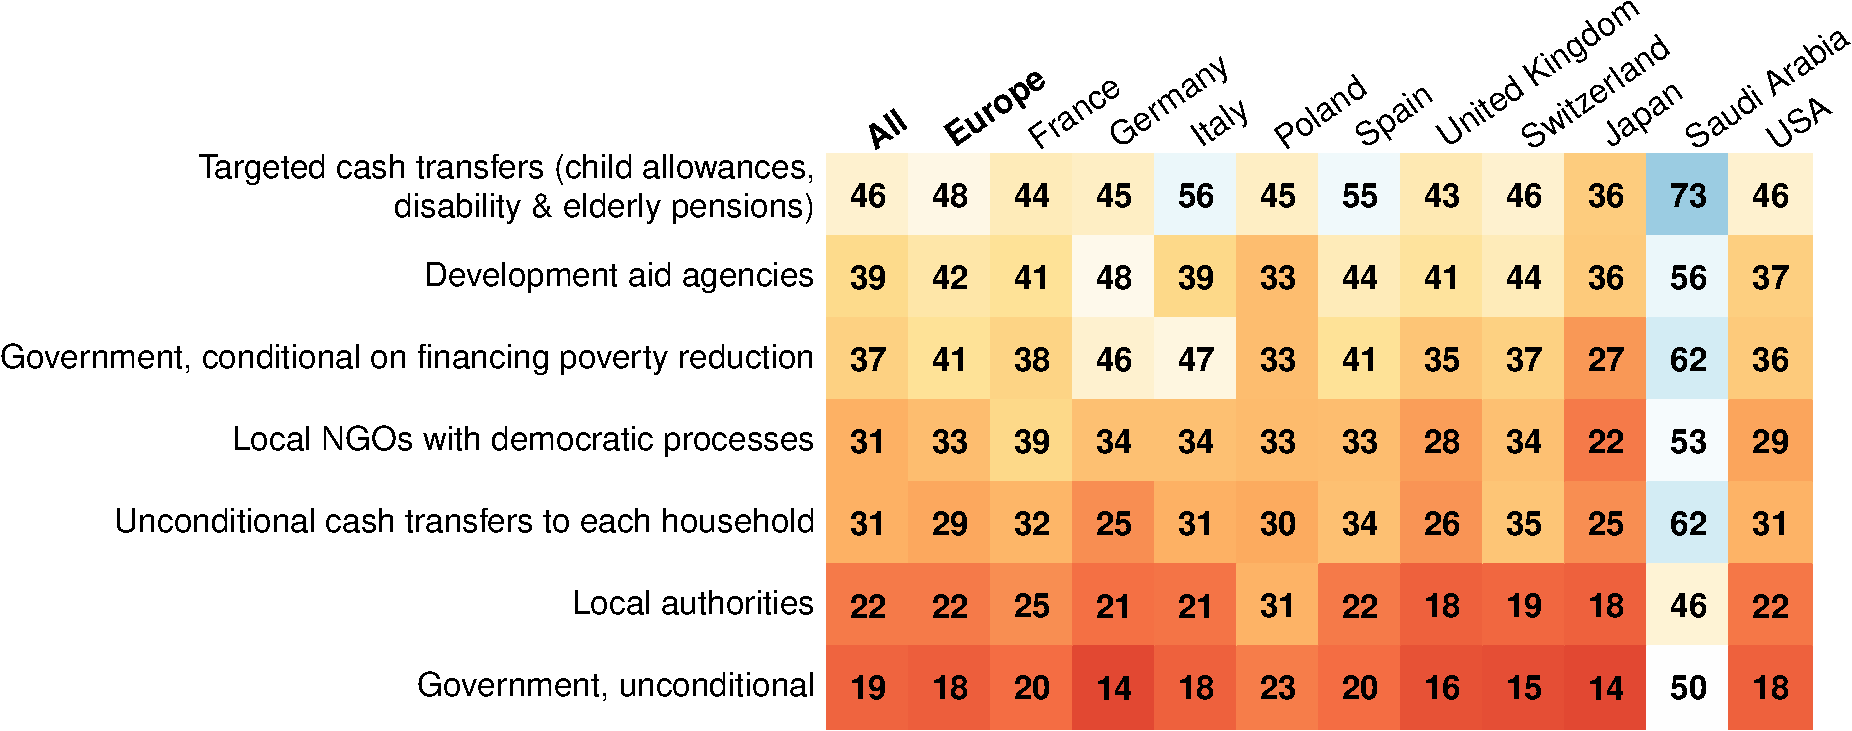
\includegraphics[width=\textwidth]{../figures/country_comparison/transfer_how_positive.pdf}} 
% % \end{figure}

% \begin{figure}[h!]
%     \caption[\textit{Best} way to transfer resources to LICs]{``How do you evaluate each of these channels to transfer resources to reduce poverty in LICs?''\\ Percentage of \textit{Best} way (other options: \textit{Right}, \textit{Wrong} or \textit{Acceptable} way). (Question~\ref{q:transfer_how}). 
    
%     \hfill (Back~to~Section~\ref{subsec:transfer_how}.)
%     }\label{fig:transfer_how_above_one}
%     \makebox[\textwidth][c]{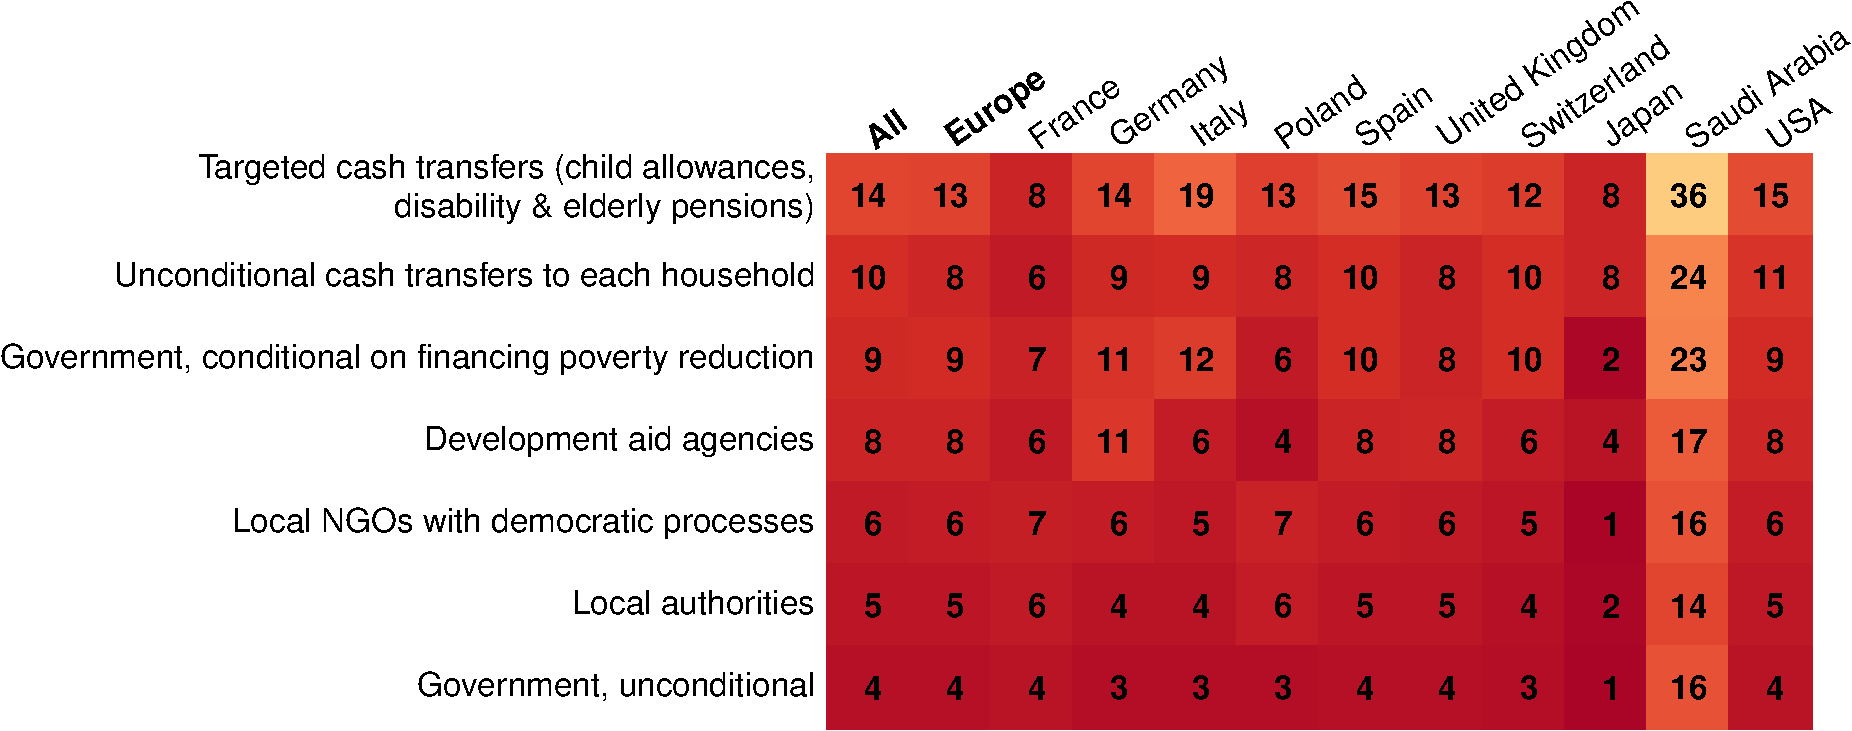
\includegraphics[width=\textwidth]{../figures/country_comparison/transfer_how_above_one.pdf}} 
% \end{figure}

% \begin{figure}[h!]
%     \caption[\textit{Wrong} way to transfer resources to LICs]{``How do you evaluate each of these channels to transfer resources to reduce poverty in LICs?''\\ Percentage of \textit{Wrong} way (other options: \textit{Best}, \textit{Right} or \textit{Acceptable} way). (Question~\ref{q:transfer_how}). 
    
%     \hfill (Back~to~Section~\ref{subsec:transfer_how}.)
%     }\label{fig:transfer_how_negative}
%     \makebox[\textwidth][c]{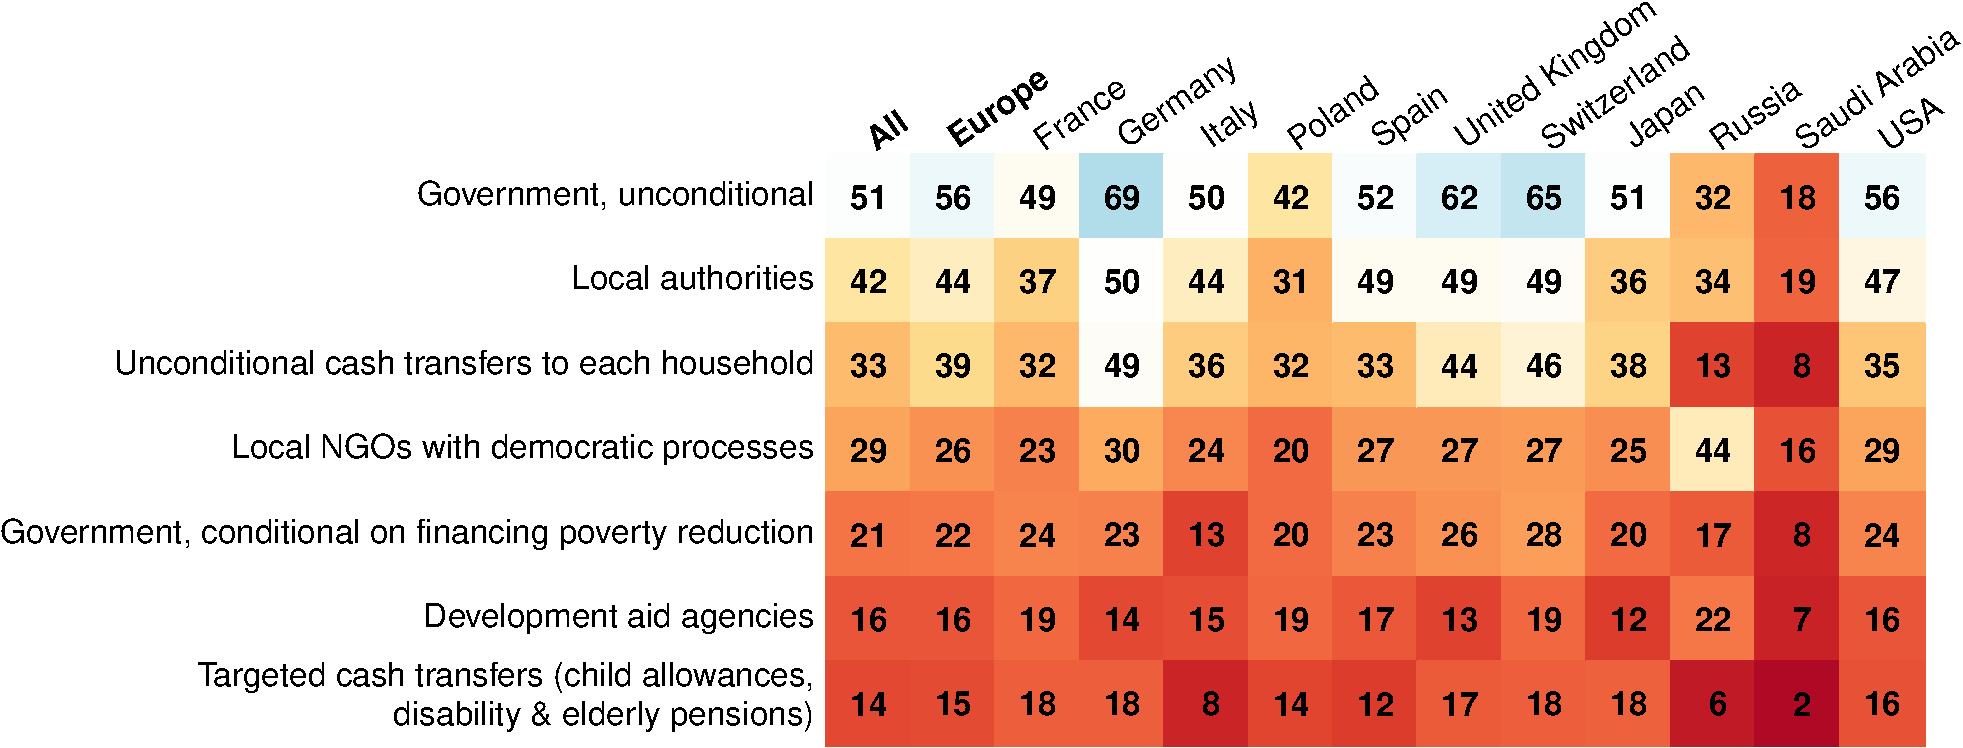
\includegraphics[width=\textwidth]{../figures/country_comparison/transfer_how_negative.pdf}} 
% \end{figure}

% \begin{figure}[h!]
%     \caption[Support for making all countries' GDP p.c. converge by 2100]{``Should governments actively cooperate to have all countries converge in terms of GDP per capita by the end of the century?'' (Question~\ref{q:convergence_support}).
%     }\label{fig:convergence_support}
%     \makebox[\textwidth][c]{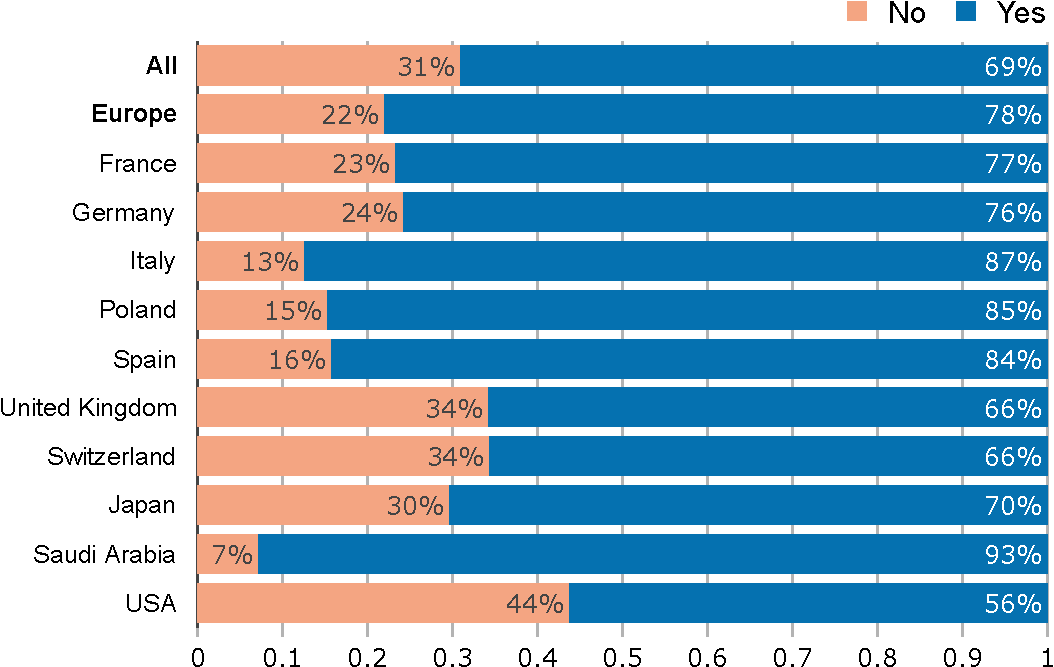
\includegraphics[width=.7\textwidth]{../figures/country_comparison/convergence_support_nolabel.pdf}} 
% \end{figure}


\begin{figure}[h!]
    \caption[Would vote for a party in a global coalition for sustainable development]{``Let us call "your political party" the party you voted for in the last election, or the party that represents your views most closely.~\\\textbf{Imagine }there was \textbf{a worldwide coalition} of political parties in favor of a common program \textbf{to tackle climate change, implement taxes on millionaires and fund poverty reduction in low-income countries}.~\\\\\textbf{Would you be more likely to vote for your party if it were part of that coalition?}'' (Question~\ref{q:vote_intl_coalition}).\hfill (Back~to~Section~\ref{par:willingness_act}.)
    }\label{fig:vote_intl_coalition}
    \makebox[\textwidth][c]{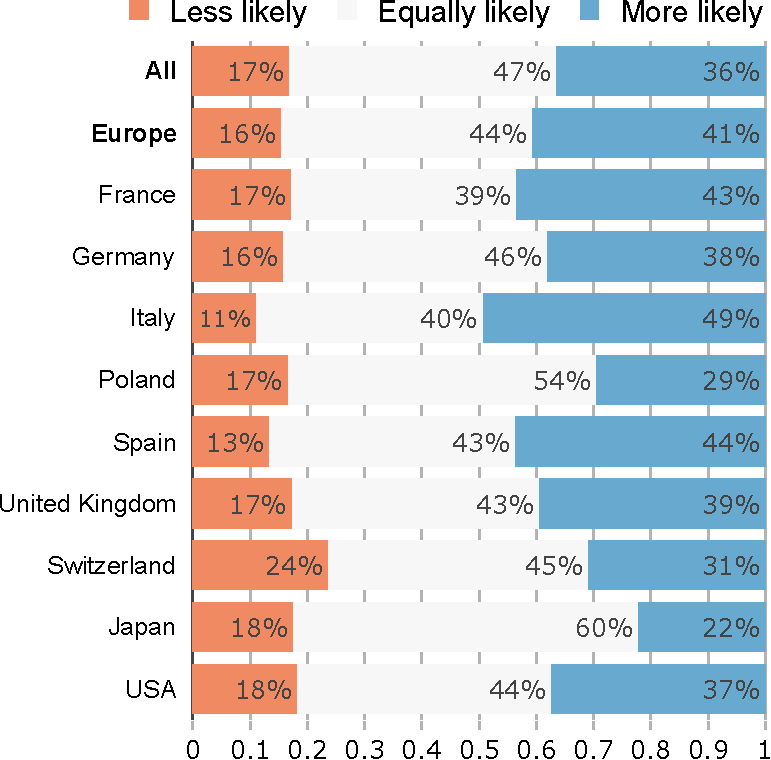
\includegraphics[width=.6\textwidth]{../figures/country_comparison/vote_intl_coalition_nolabel.pdf}} 
\end{figure}

\begin{figure}[h!]
    \caption[Agreement with rationales for global redistribution]{``Some people think that high-income countries should support low-income countries.~\\Among the different reasons given, which ones do you agree with? (Multiple answers possible)'' (Question~\ref{q:why_hic_help_lic}).\hfill (Back~to~Section~\ref{par:why_help_lic}.)
    }\label{fig:why_hic_help_lic}
    \makebox[\textwidth][c]{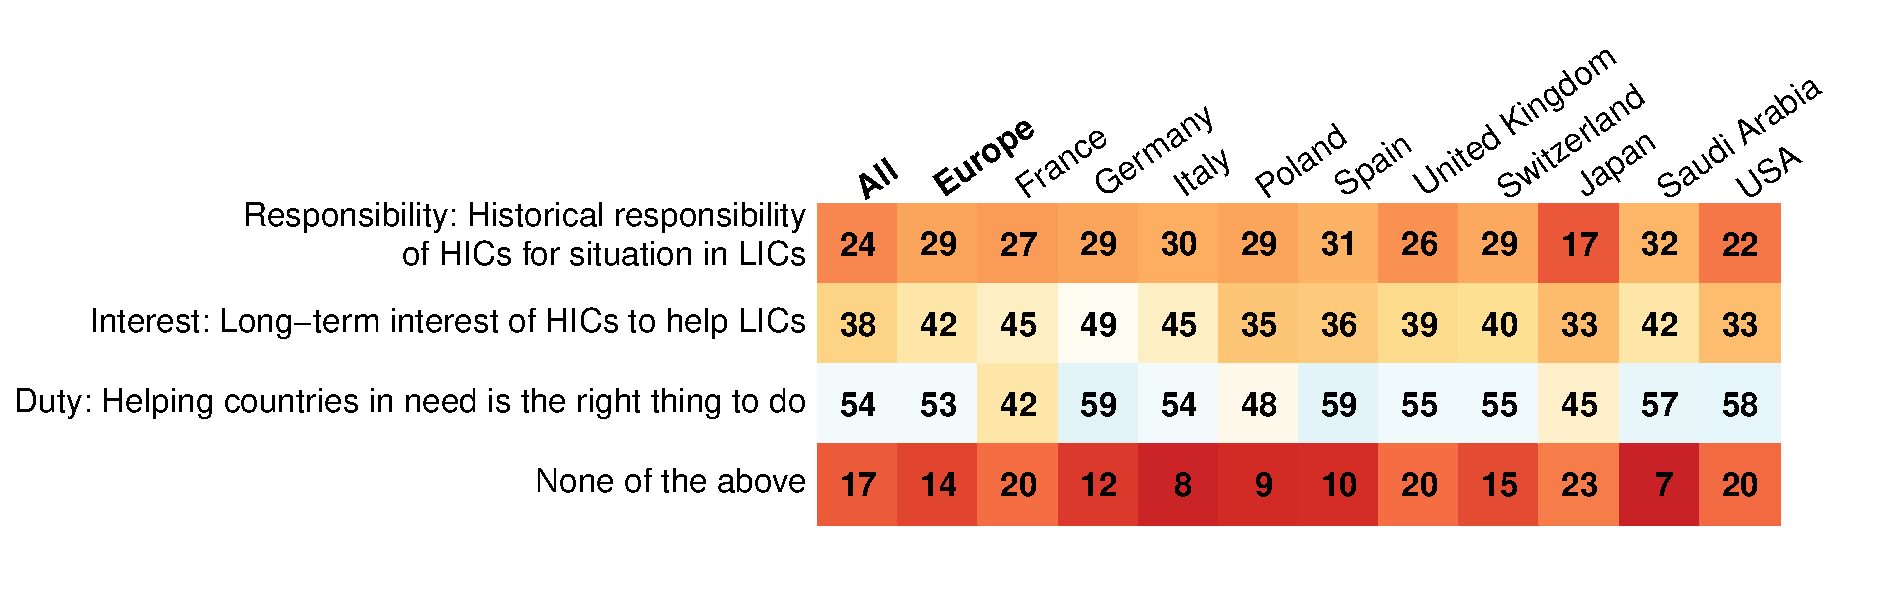
\includegraphics[width=\textwidth]{../figures/country_comparison/why_hic_help_lic_positive.pdf}} 
\end{figure}

\begin{figure}[h!]
    \caption[Support for reparations for colonization and slavery]{``Some people argue that Western countries owe reparations for colonization and slavery to former colonies and descendants of slaves. \\Reparations could take the form of funding education and facilitating technology transfers, to address unequal opportunities passed down from the past. \\\\\textbf{Do you support or oppose reparations} of this kind \textbf{for colonization and slavery?~}'' (Question~\ref{q:reparations_support}).\hfill (Back~to~Section~\ref{par:reparations}.)
    }\label{fig:reparations_support}
    \makebox[\textwidth][c]{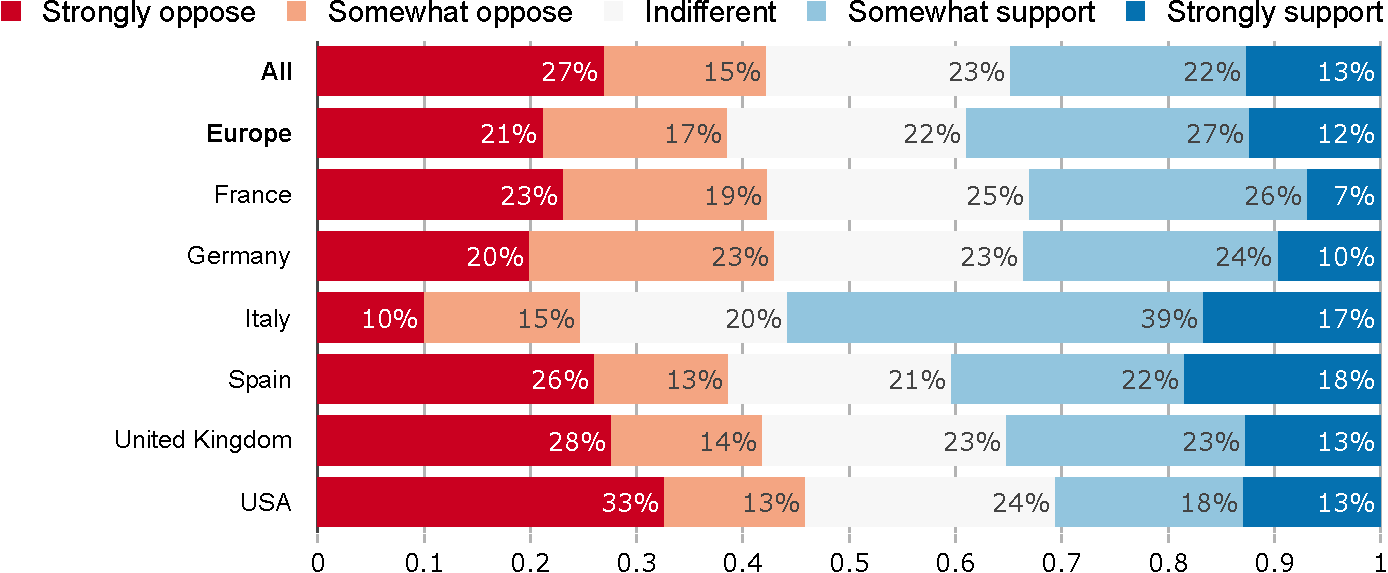
\includegraphics[width=.9\textwidth]{../figures/country_comparison/reparations_support_nolabel.pdf}} 
\end{figure}

\begin{figure}[h!]
    \caption[Median custom redistribution]{Global redistribution obtained from median custom parameters: 49\% of winners; 18\% of losers; degree of redistribution of 5 (out of 10). (Question~\ref{q:custom_redistr}).\hfill (Section~\ref{subsec:custom_redistr}.)
    }\label{fig:custom_redistr_median}
    \makebox[\textwidth][c]{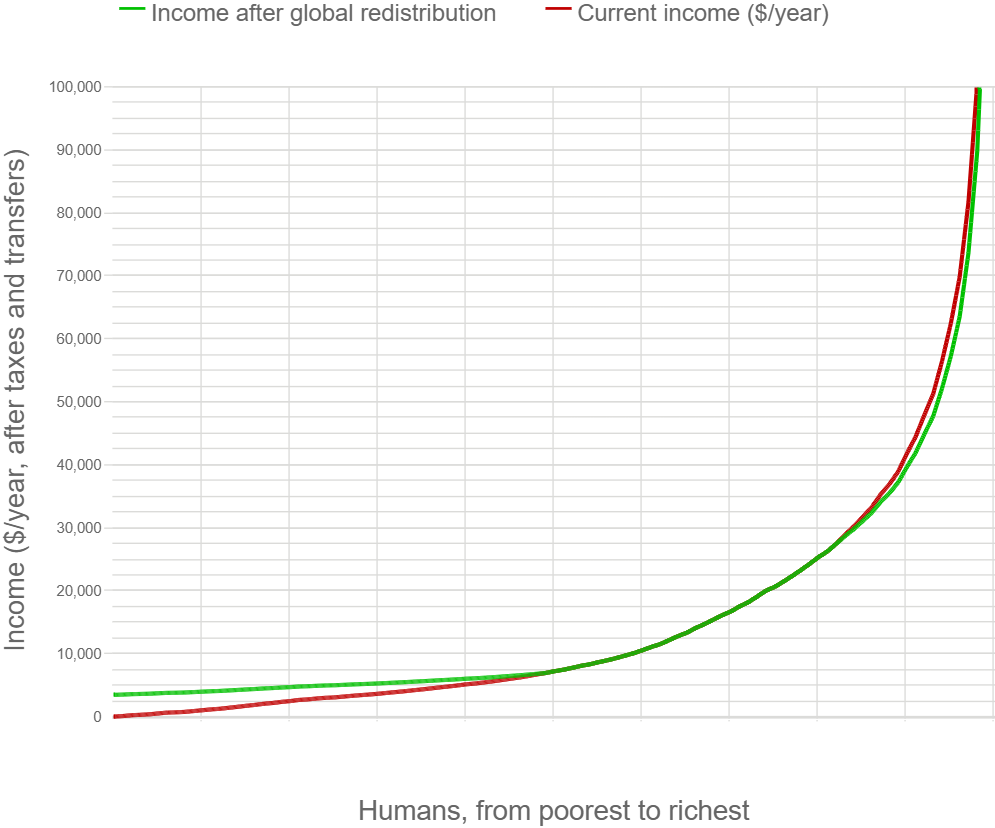
\includegraphics[width=.9\textwidth]{../figures/questionnaire/survey_custom_redistr_median_zoom.png}} 
\end{figure} 

\begin{figure}[h!]
    \caption[Average custom redistribution]{Average custom global redistribution. (Question~\ref{q:custom_redistr}).\hfill (Back~to~Section~\ref{subsec:custom_redistr}.)
    }\label{fig:custom_redistr_mean}
    \makebox[\textwidth][c]{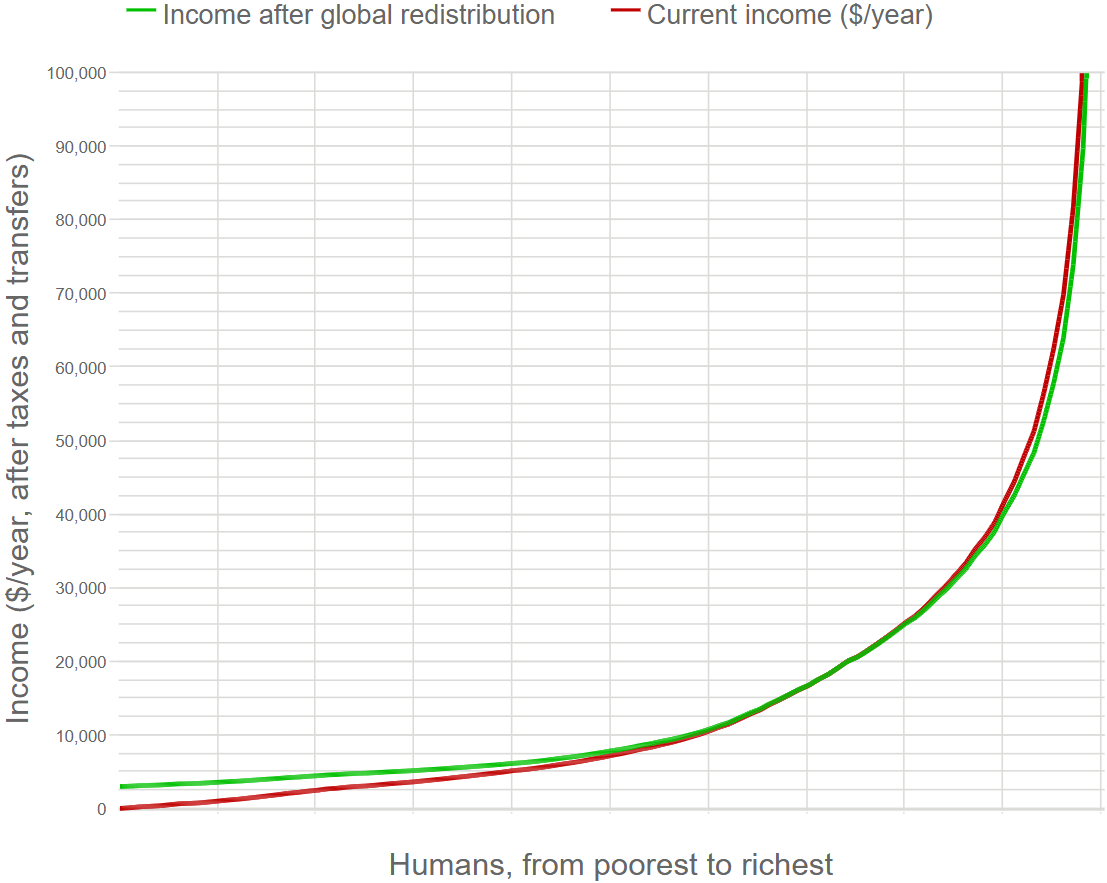
\includegraphics[width=.9\textwidth]{../figures/mean_custom_redistr/all_satisfied.png}} 
\end{figure}

% \begin{figure}[h!]
%     \caption[Average answers to custom redistribution]{Mean answers to custom redistribution. (Question~\ref{q:custom_redistr}).\hfill (Back~to~Section~\ref{subsec:custom_redistr}.)
%     }\label{fig:custom_redistr_most}
%     \makebox[\textwidth][c]{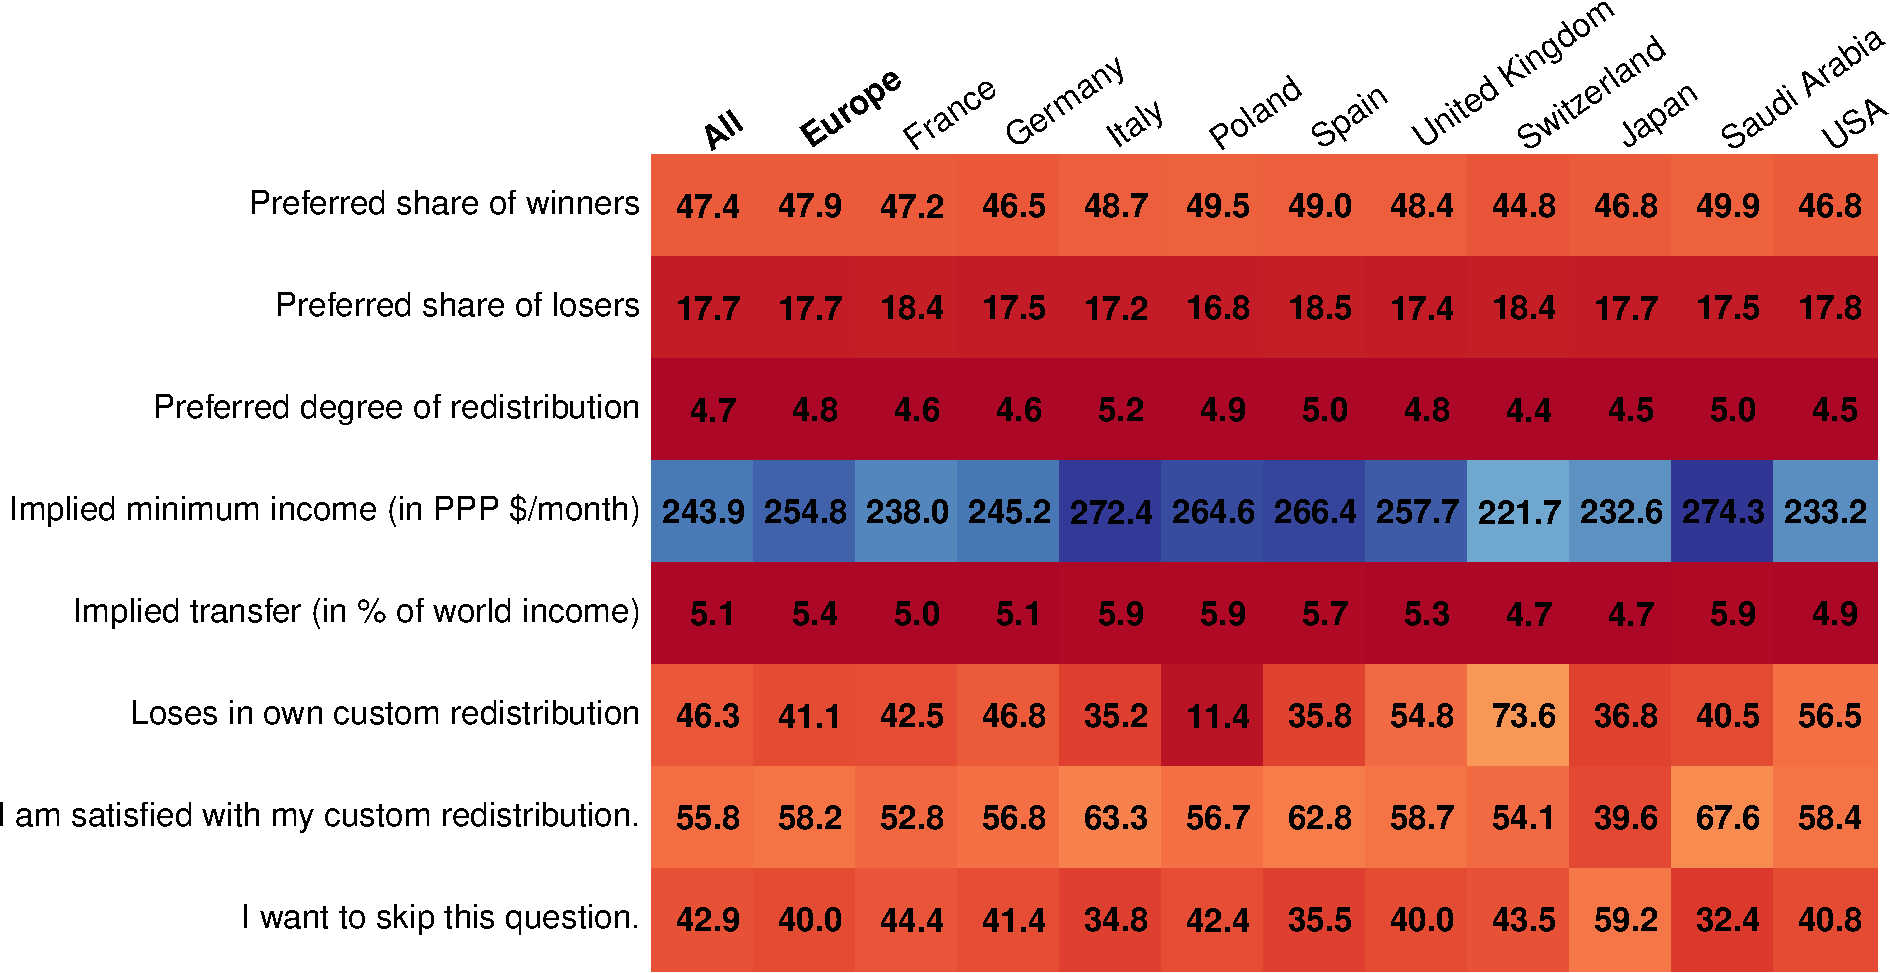
\includegraphics[width=\textwidth]{../figures/country_comparison/custom_redistr_most_mean.pdf}} 
% \end{figure} 

% \begin{figure}[h!]
%     \caption[Average answers to custom redistribution among satisfied]{Mean answers to custom redistribution among respondents satisfied with their custom redistribution. (Question~\ref{q:custom_redistr}).\hfill (Back~to~Section~\ref{subsec:custom_redistr}.)
%     }\label{fig:custom_redistr_satisfied_mean}
%     \makebox[\textwidth][c]{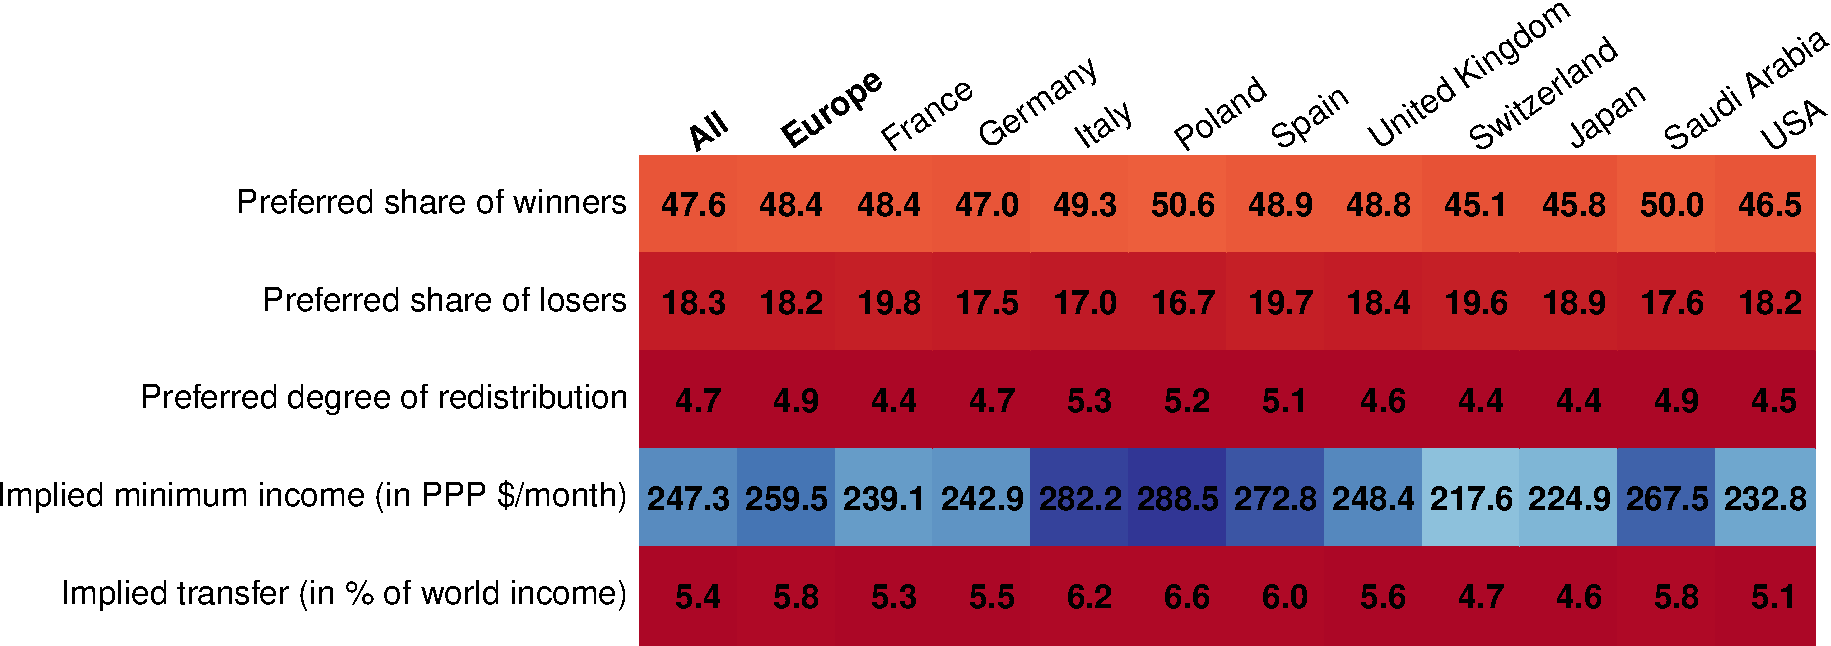
\includegraphics[width=\textwidth]{../figures/country_comparison/custom_redistr_satisfied_mean.pdf}} 
% \end{figure} 

% \begin{figure}[h!]
%     \caption[Median answers to custom redistribution among satisfied]{Median answers to custom redistribution among respondents satisfied with their custom redistribution. (Question~\ref{q:custom_redistr}).\hfill (Back~to~Section~\ref{subsec:custom_redistr}.)
%     }\label{fig:custom_redistr_satisfied_median}
%     \makebox[\textwidth][c]{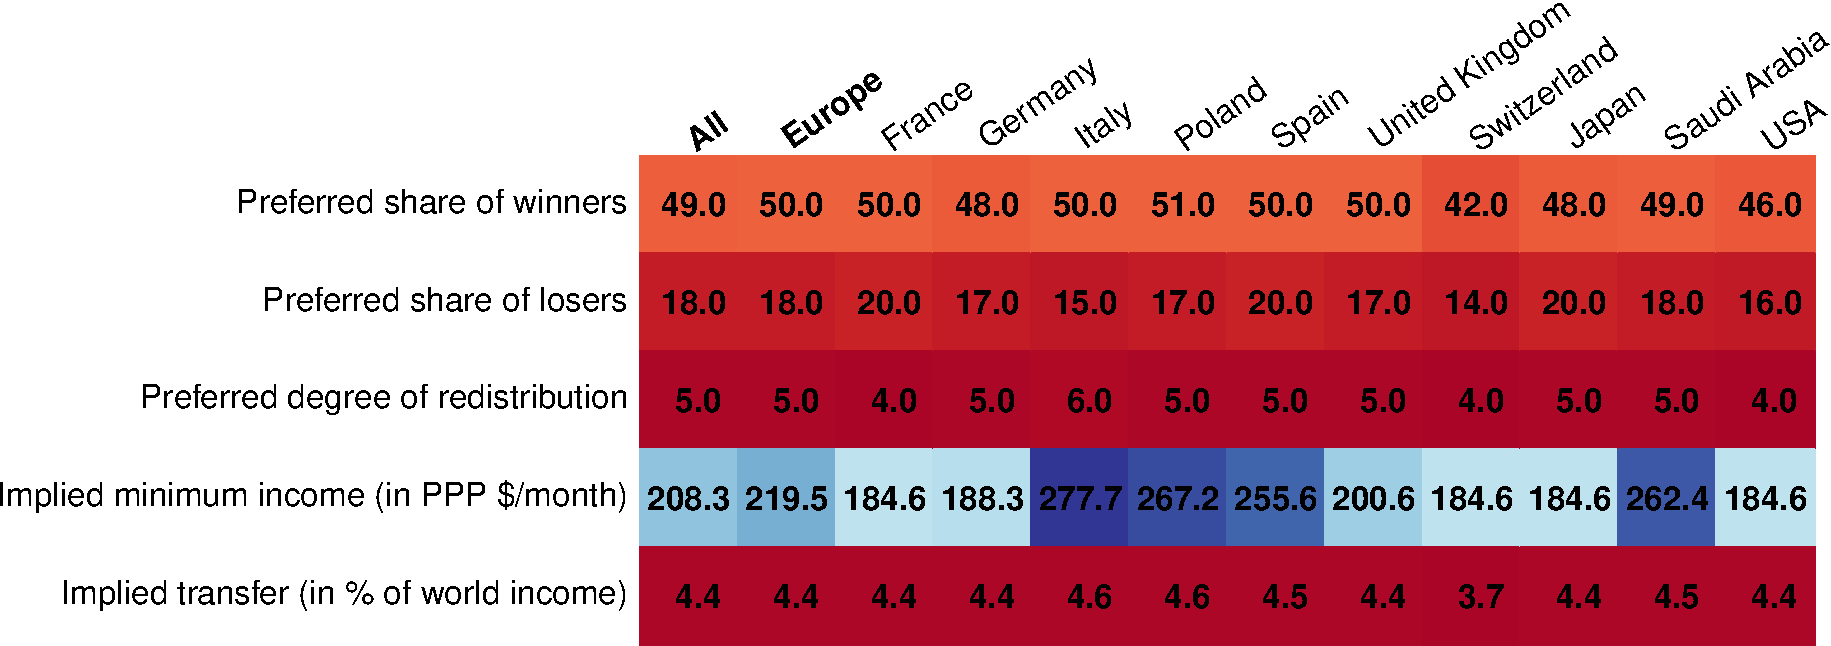
\includegraphics[width=\textwidth]{../figures/country_comparison/custom_redistr_satisfied_median.pdf}} 
% \end{figure} 

% \begin{figure}[h!]
%     \caption[Preferred share of winners in the custom redistributions]{Preferred share of winners in the custom redistributions among satisfied respondents. (Question~\ref{q:custom_redistr}).\hfill (Back~to~Section~\ref{subsec:custom_redistr}.)
%     }\label{fig:custom_redistr_winners_agg}
%     \makebox[\textwidth][c]{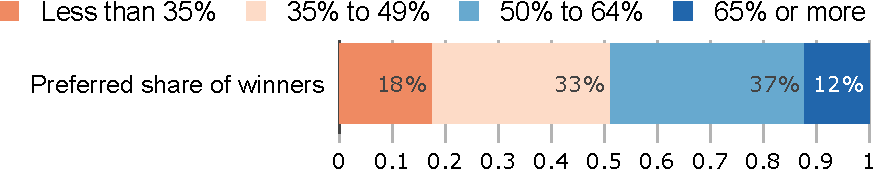
\includegraphics[width=.8\textwidth]{../figures/all/custom_redistr_winners_agg.pdf}} 
% \end{figure} 

% \begin{figure}[h!]
%     \caption[Preferred share of losers in the custom redistributions]{Preferred share of losers in the custom redistributions among satisfied respondents. (Question~\ref{q:custom_redistr}).\hfill (Back~to~Section~\ref{subsec:custom_redistr}.)
%     }\label{fig:custom_redistr_losers_agg}
%     \makebox[\textwidth][c]{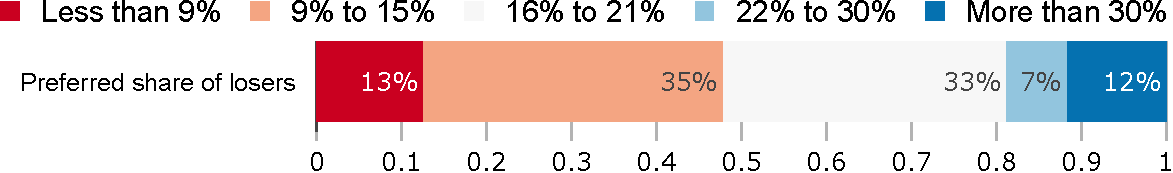
\includegraphics[width=\textwidth]{../figures/all/custom_redistr_losers_agg.pdf}} 
% \end{figure} 

% \begin{figure}[h!]
%     \caption[Minimum income implied by custom redistributions]{Minimum worldwide income implied by custom redistributions among satisfied respondents (in PPP \$ per month). (Question~\ref{q:custom_redistr}).\hfill (Back~to~Section~\ref{subsec:custom_redistr}.)
%     }\label{fig:custom_redistr_income_min_ceiling}
%     \makebox[\textwidth][c]{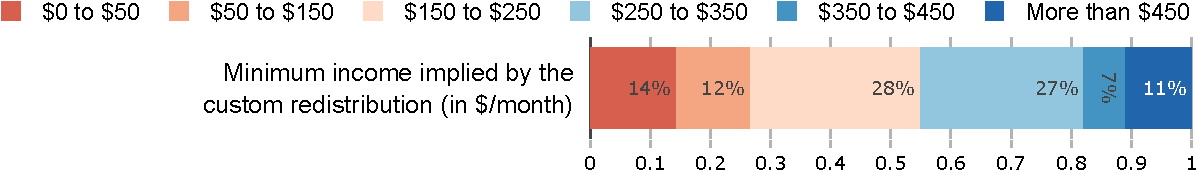
\includegraphics[width=\textwidth]{../figures/all/custom_redistr_income_min_ceiling.pdf}} 
% \end{figure} 

% \begin{figure}[h!]
%     \caption[Transfer implied by custom redistributions]{Rich-to-poor transfer implied by custom redistributions among satisfied respondents. (Question~\ref{q:custom_redistr}).\hfill (Back~to~Section~\ref{subsec:custom_redistr}.)
%     }\label{fig:custom_redistr_transfer_ceiling}
%     \makebox[\textwidth][c]{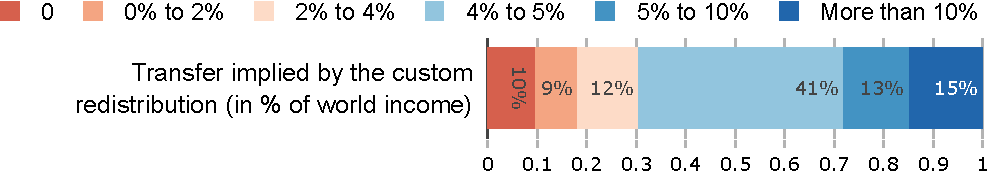
\includegraphics[width=.9\textwidth]{../figures/all/custom_redistr_transfer_ceiling.pdf}} 
% \end{figure} 

% % \begin{figure}[h!]
% %     \caption[Average well-being depending on the variant]{Average subjective well-being, depending on the variant. (Question~\ref{q:well_being}).
% %     }\label{fig:well_being}
% %     \makebox[\textwidth][c]{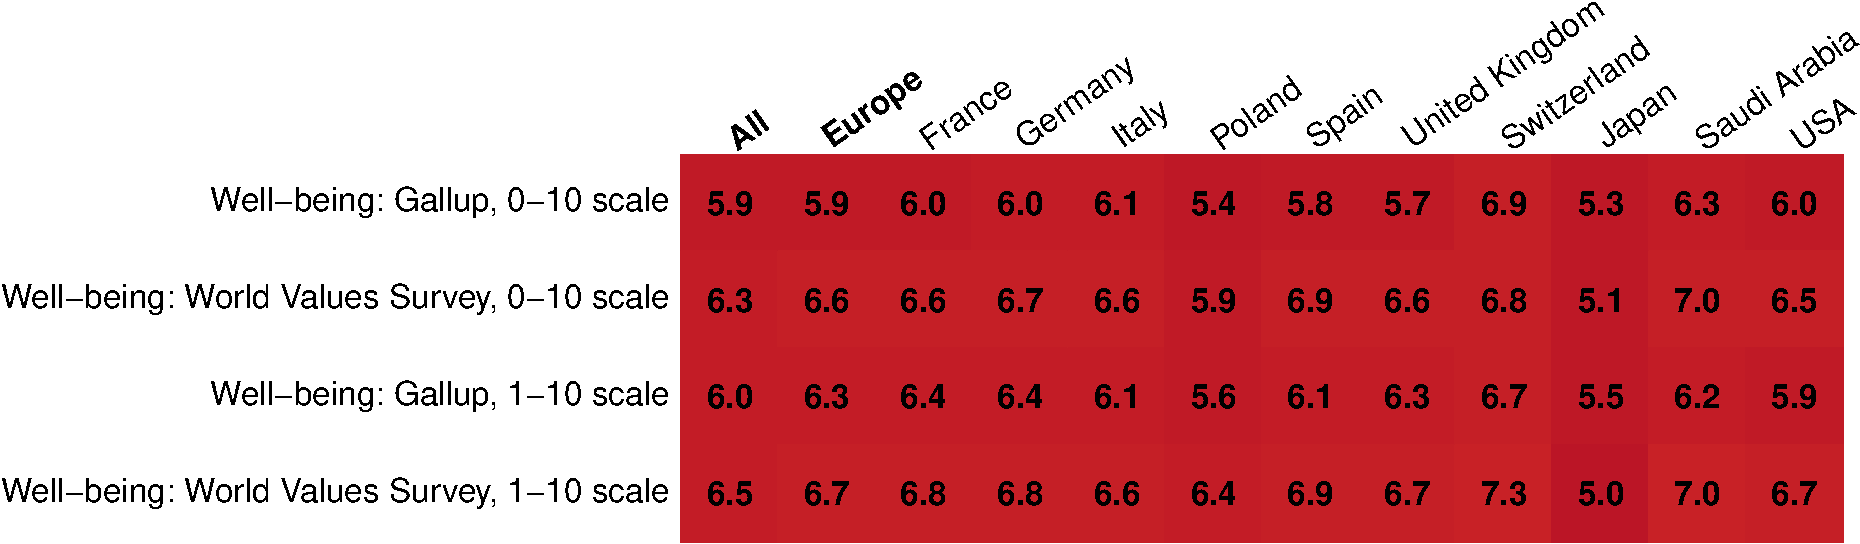
\includegraphics[width=\textwidth]{../figures/country_comparison/well_being_mean.pdf}} 
% % \end{figure}

% \begin{figure}[h!]
%     \caption[Comprehension question on GCS]{``\textit{Comprehension question: one respondent with the expected answer will get [amount\_lottery: \$100].}\\\\How would gasoline prices change as a result of the Global Climate Scheme? \\Gasoline prices would...'' (Correct answer: \textit{increase}) (Question~\ref{q:gcs_comprehension}).
%     }\label{fig:gcs_comprehension}
%     \makebox[\textwidth][c]{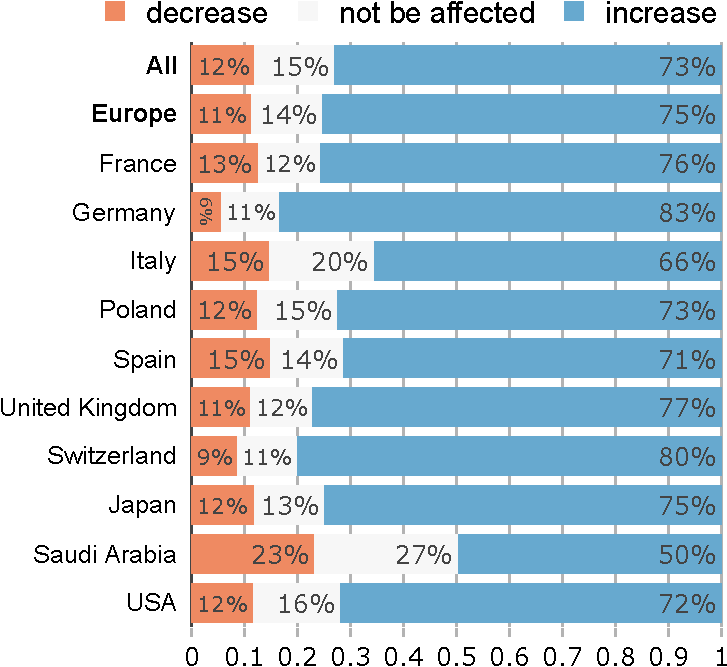
\includegraphics[width=.5\textwidth]{../figures/country_comparison/gcs_comprehension_nolabel.pdf}} 
% \end{figure}

% \begin{figure}[h!]
%     \caption[Relative agreement: ``My taxes should go towards solving global problems'']{Relative agreement for: ``To what extent do you agree or disagree with the following statement? "My taxes should go towards solving global problems."'' (Percentage of \textit{Agree} or \textit{Strongly agree} among non-\textit{Neither agree nor disagree} responses). (Question~\ref{q:my_tax_global_nation}).
%     }\label{fig:my_tax_global_nation_share}
%     \makebox[\textwidth][c]{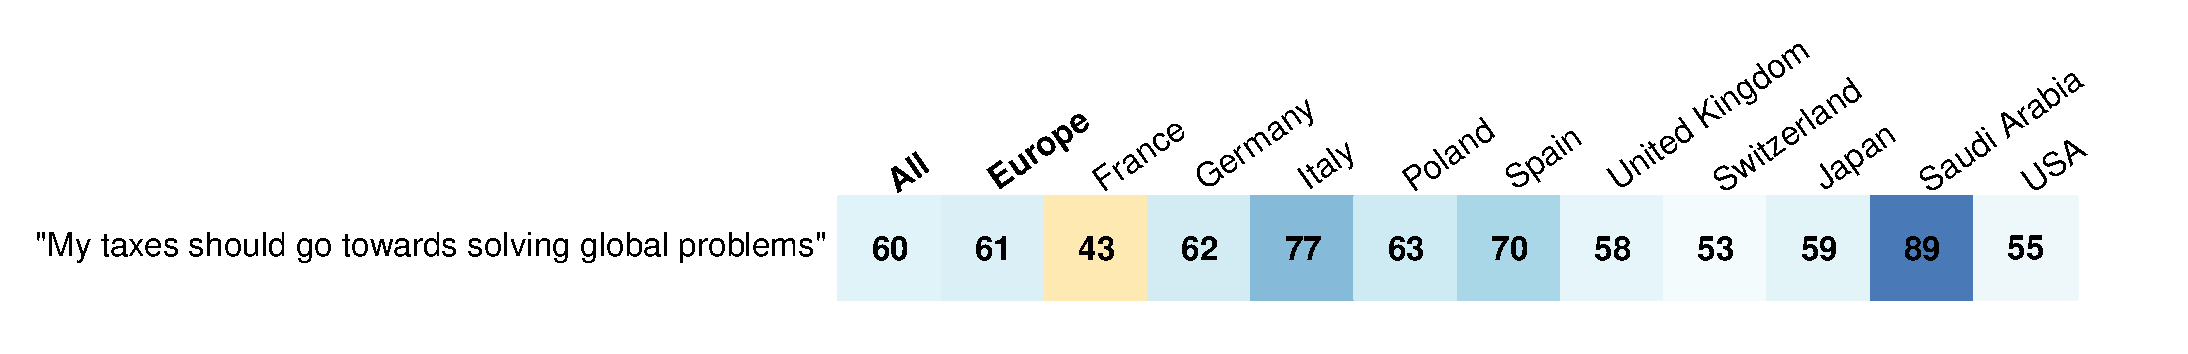
\includegraphics[width=\textwidth]{../figures/country_comparison/my_tax_global_nation_share.pdf}} 
% \end{figure}

% \begin{figure}[h!]
%     \caption[Absolute agreement: ``My taxes should go towards solving global problems'']{Absolute agreement for: ``To what extent do you agree or disagree with the following statement? "My taxes should go towards solving global problems."'' (Percentage of \textit{Agree} or \textit{Strongly agree}). (Question~\ref{q:my_tax_global_nation}).
%     }\label{fig:my_tax_global_nation_positive}
%     \makebox[\textwidth][c]{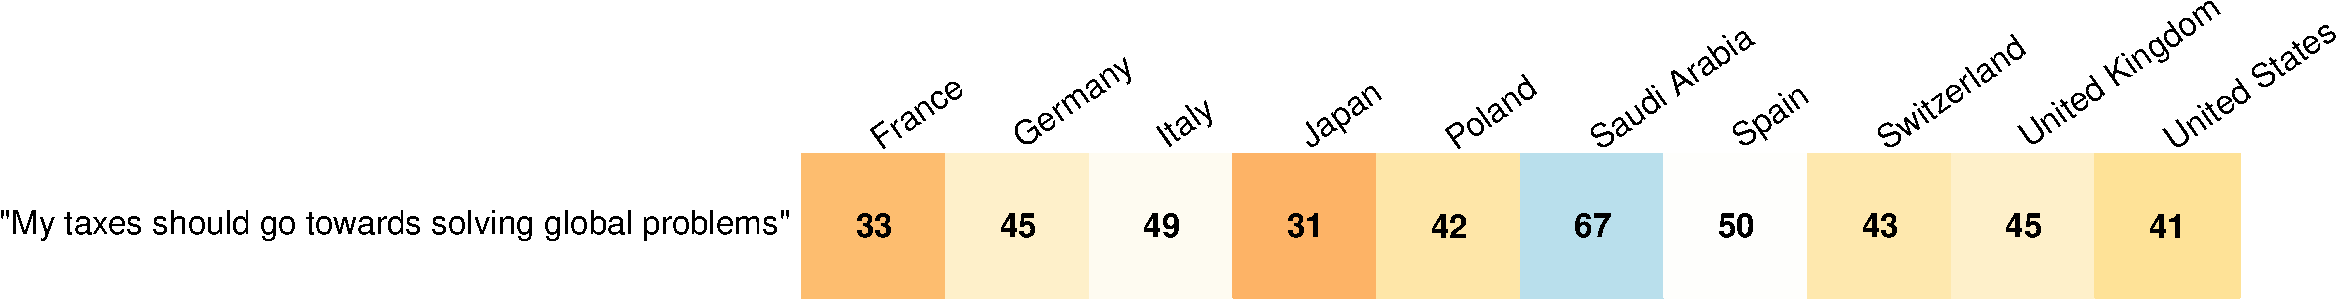
\includegraphics[width=\textwidth]{../figures/country_comparison/my_tax_global_nation_positive.pdf}} 
% \end{figure}

\begin{figure}[h!]
    \caption[Moral circle]{``Which group of people do you advocate for when you vote?''\footref{fn:group_defended} (Question~\ref{q:group_defended}).\hfill (Back~to~Section~\ref{par:group_defended}.)
    }\label{fig:group_defended_all}
    \makebox[\textwidth][c]{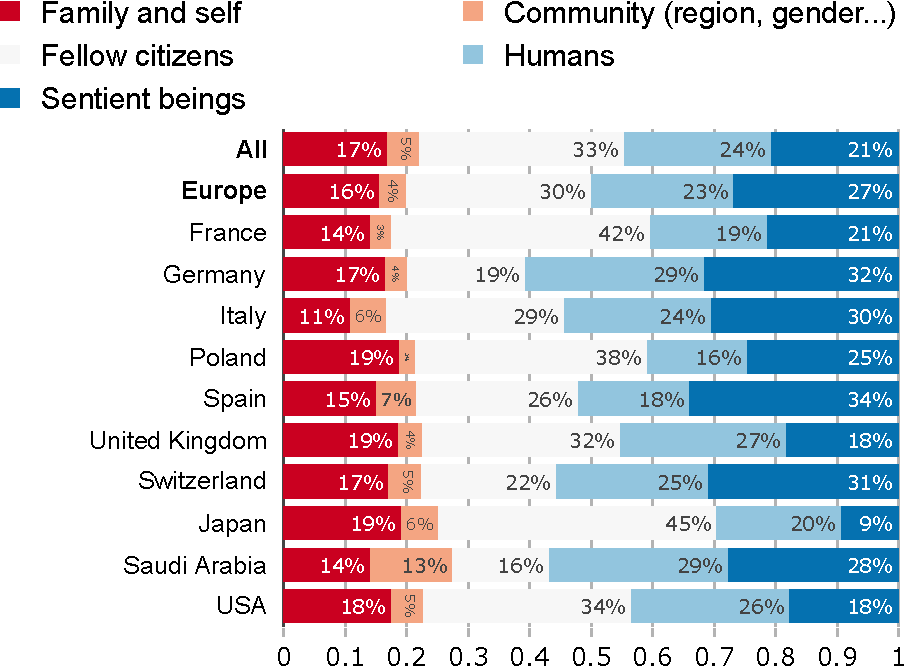
\includegraphics[width=.9\textwidth]{../figures/country_comparison/group_defended_nolabel.pdf}} 
\end{figure}

% % \begin{figure}[h!]
% %     \caption[Moral circle (heatmap)]{``Which group of people do you advocate for when you vote?'' (Question~\ref{q:group_defended}).
% %     }\label{fig:group_defended_heatmap}
% %     \makebox[\textwidth][c]{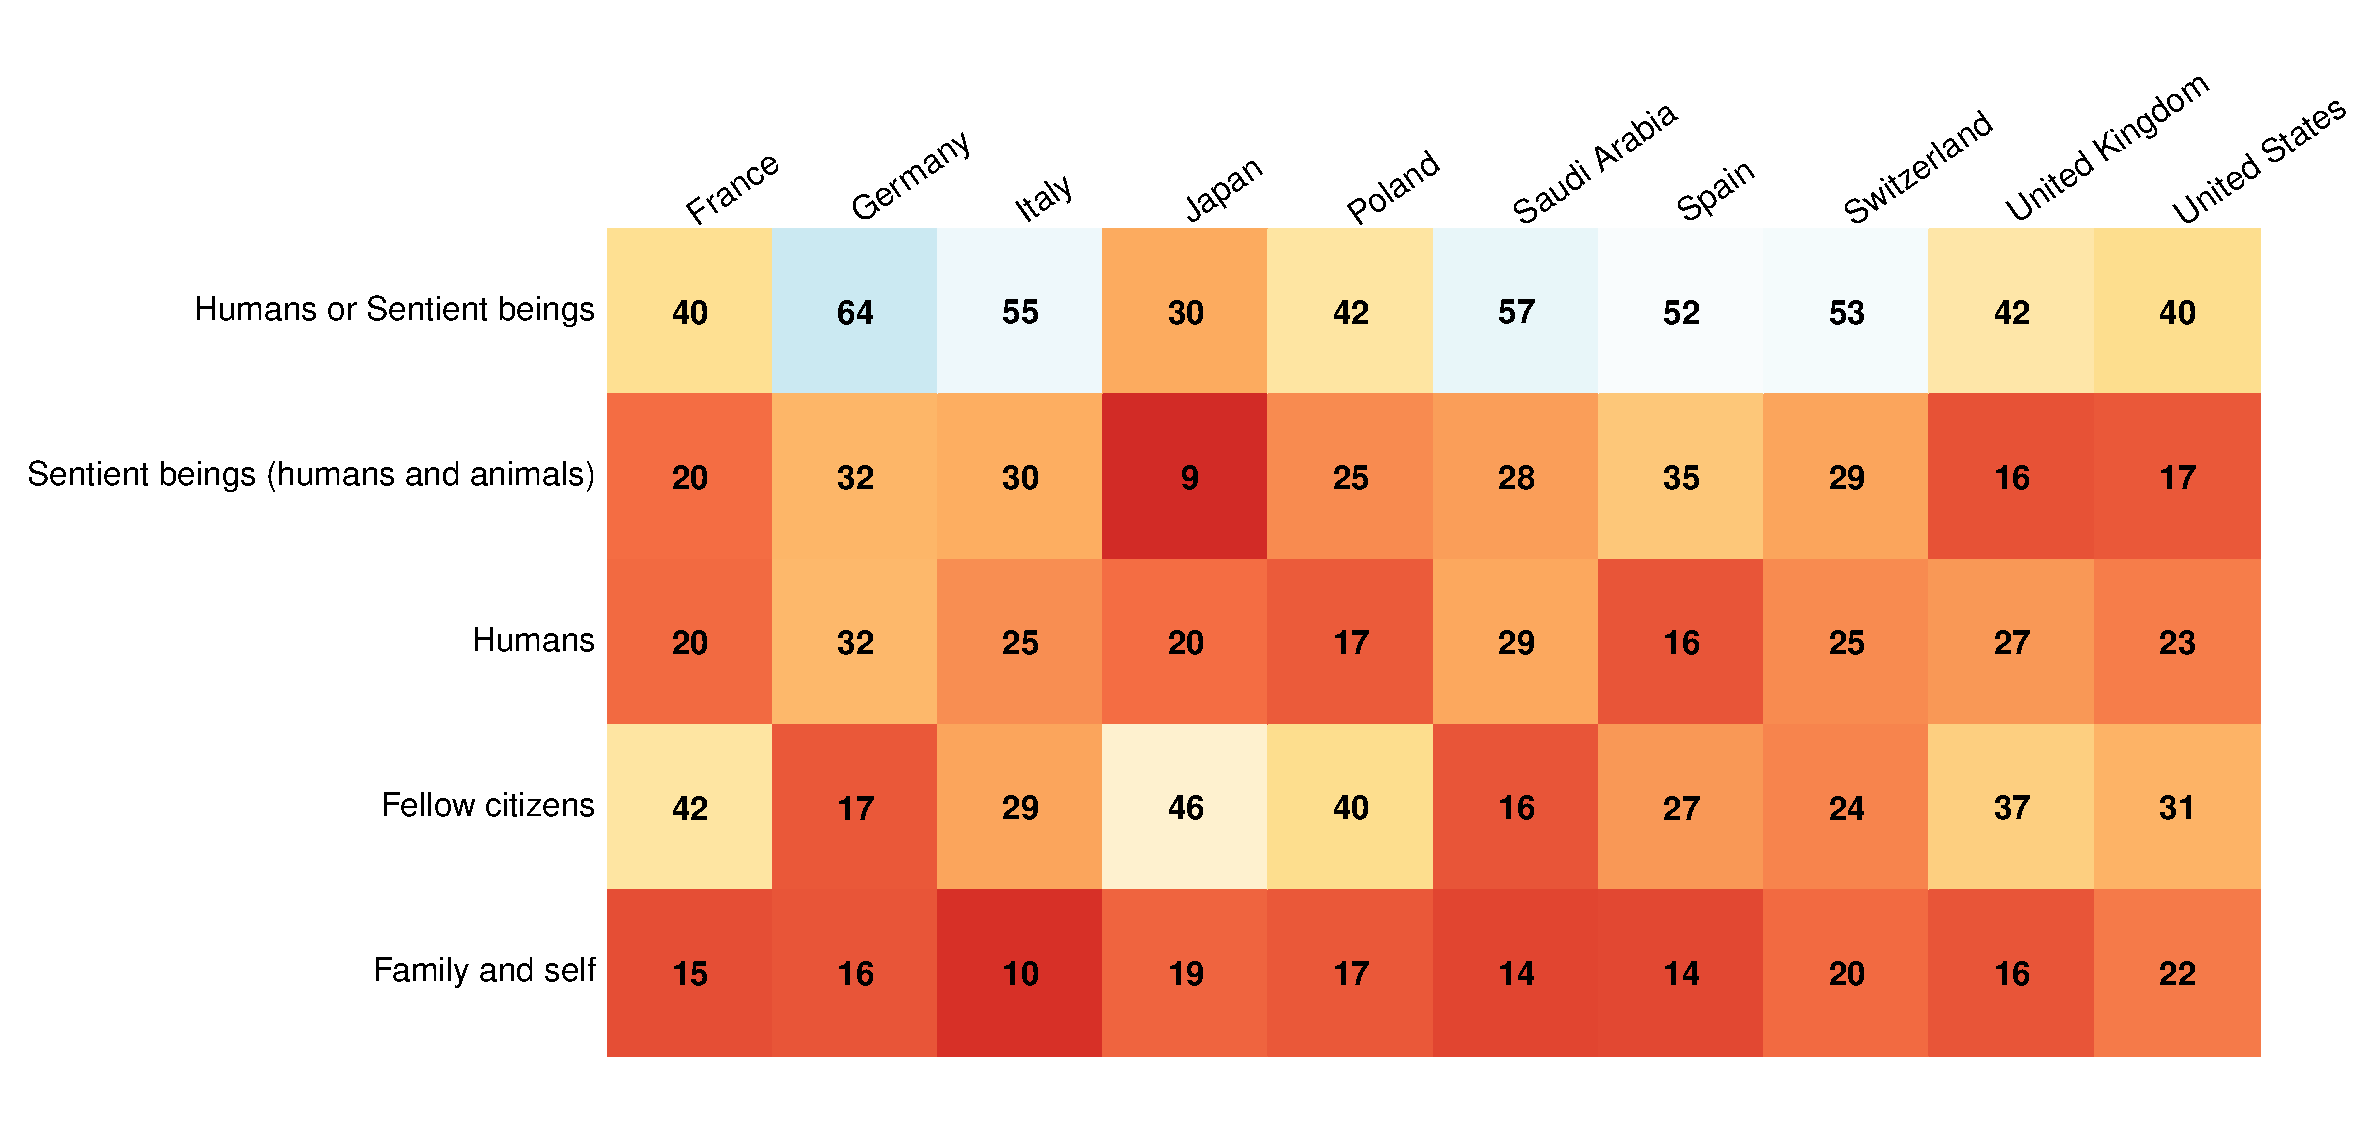
\includegraphics[width=.9\textwidth]{../figures/country_comparison/group_defended_5_positive.pdf}} 
% % \end{figure}

\begin{figure}[h!]
    \caption[Feeling that the survey was politically biased]{``Do you feel that this survey was politically biased?'' (Question~\ref{q:survey_biased}).\hfill (Back~to~Section~\ref{par:data_quality}.)
    }\label{fig:survey_biased}
    \makebox[\textwidth][c]{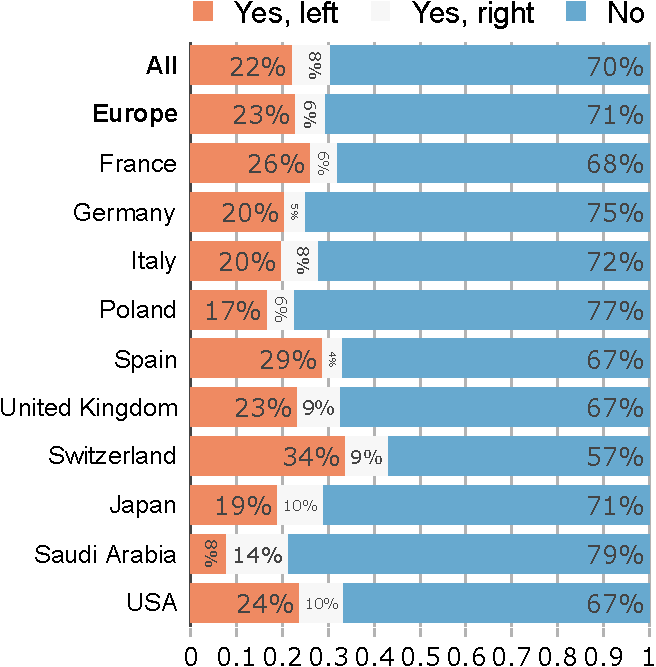
\includegraphics[width=.5\textwidth]{../figures/country_comparison/survey_biased_nolabel.pdf}} 
\end{figure}

% \begin{figure}[h!]
%     \caption[Manual classification of \textit{feedback} fields]{Manual classification of \textit{feedback} fields: ``The survey is nearing completion. You can now enter any comments, thoughts, or suggestions in the field below.'' (Question~\ref{q:comment_field}).\hfill (Back~to~Section~\ref{par:data_quality}.)
%     }\label{fig:comment_field}
%     \makebox[\textwidth][c]{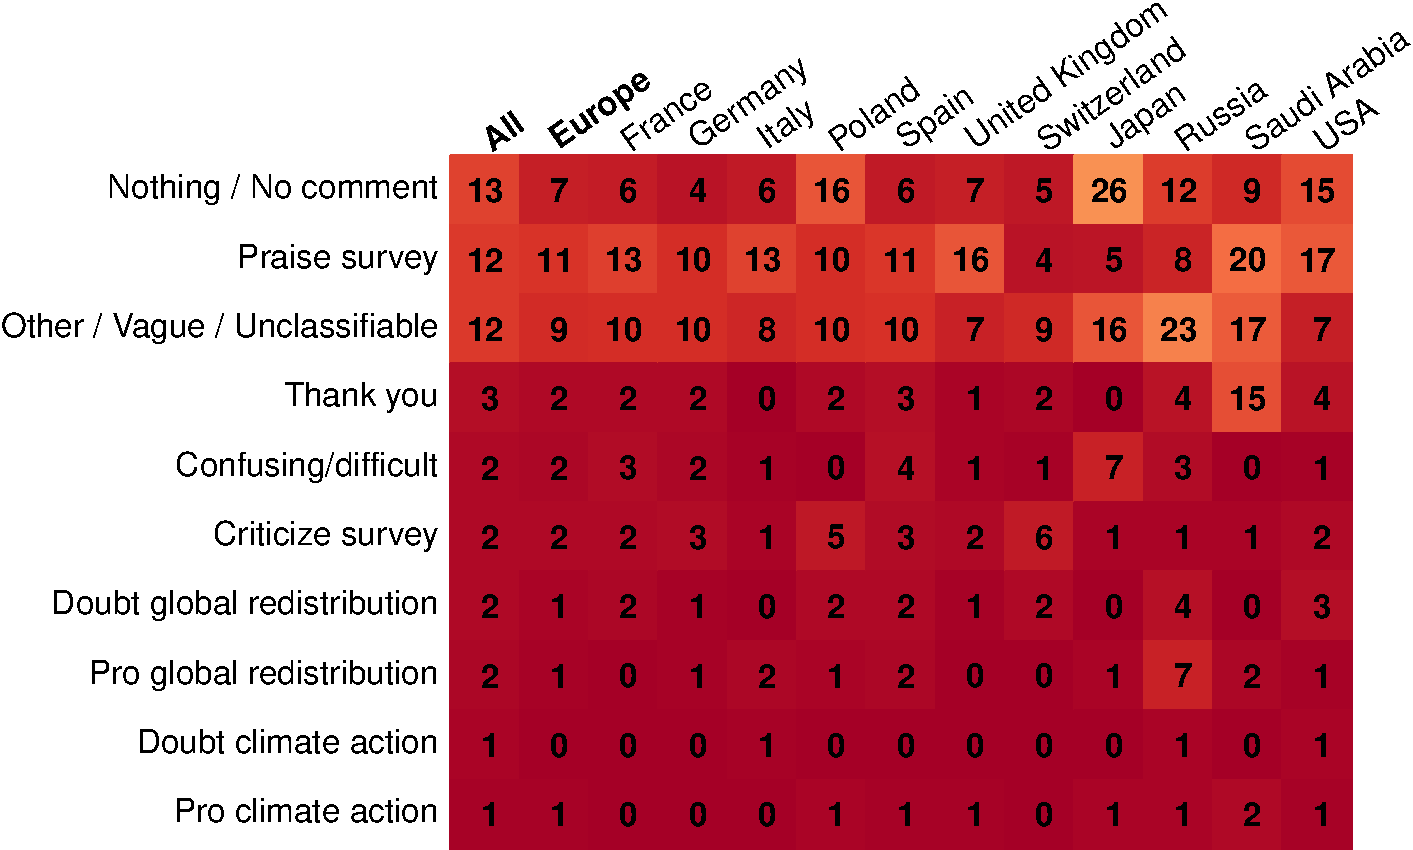
\includegraphics[width=.9\textwidth]{../figures/country_comparison/comment_manual_positive.pdf}} 
% \end{figure}

% % \begin{figure}[h!]
% %     \caption[]{. (Questions~\ref{q:gcs_support}).
% %     }\label{fig:radical_redistr_positive}
% %     \makebox[\textwidth][c]{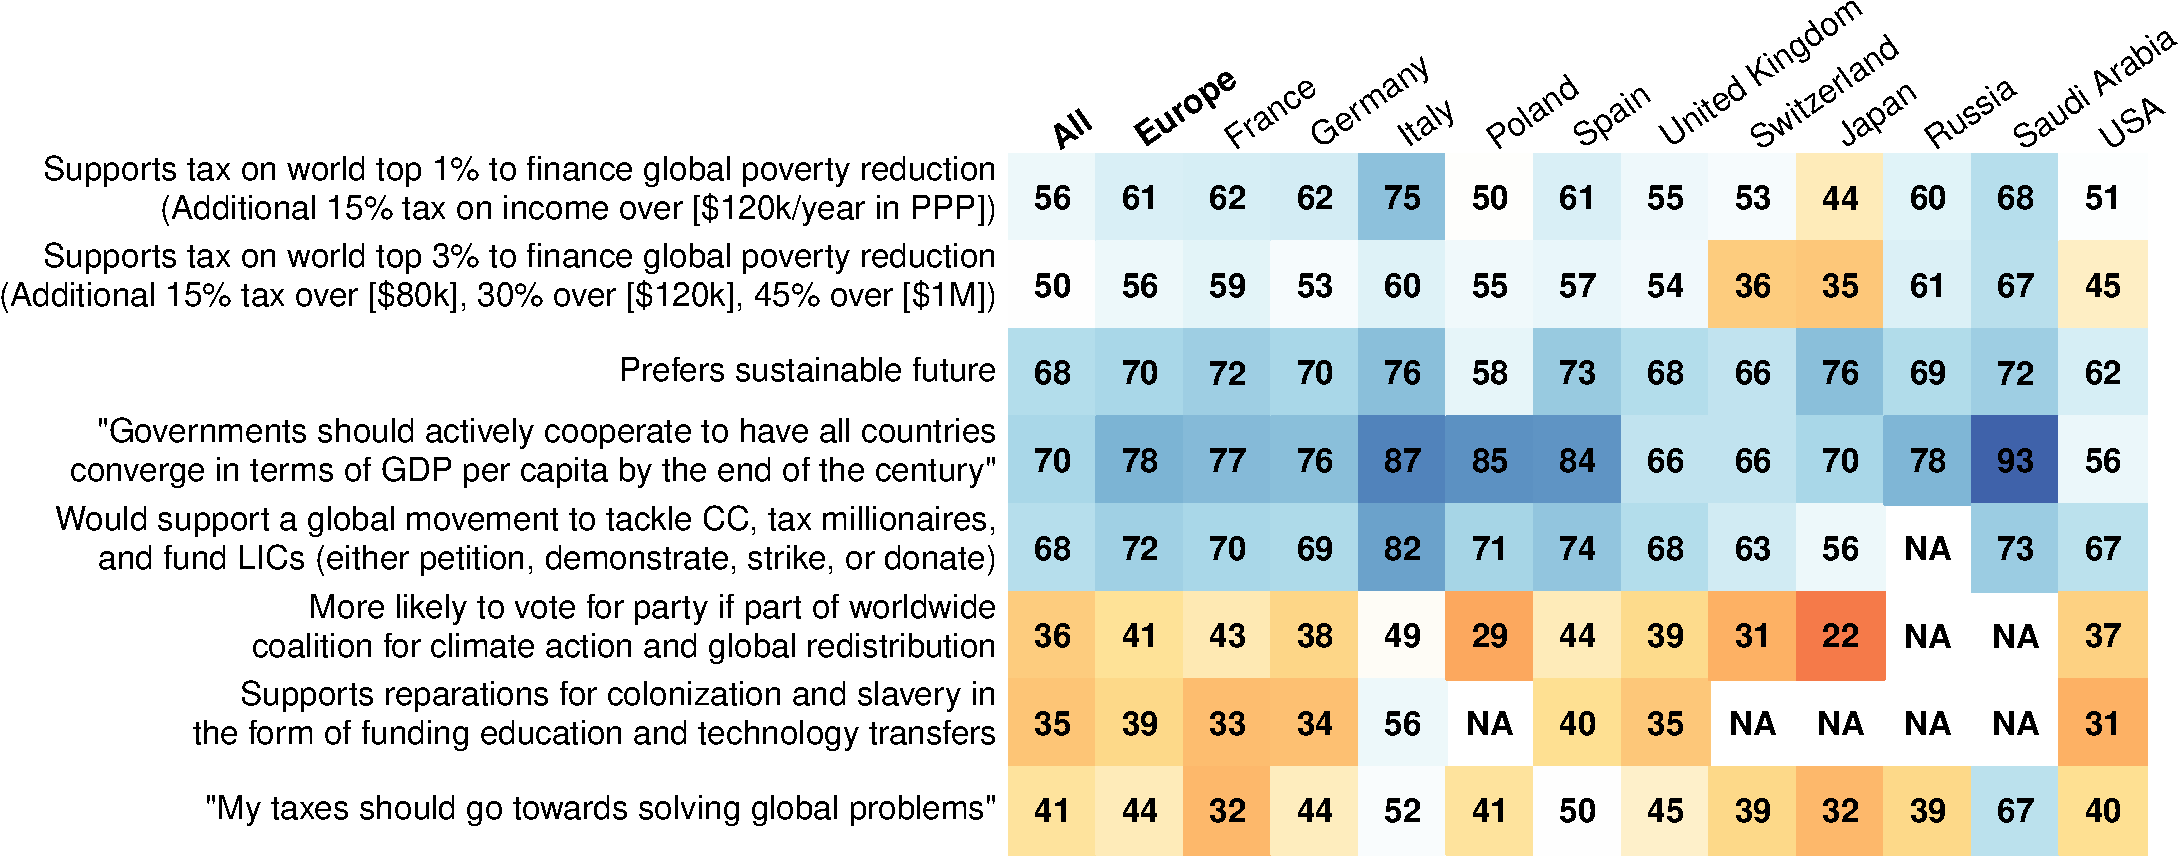
\includegraphics[width=.9\textwidth]{../figures/country_comparison/radical_redistr_positive.pdf}} 
% % \end{figure} % TODO?

% % Pb of translation in Saudi Arabia: millionaire has probably be understood in SAR (= $250k)
% \begin{figure}[h!]
%     \caption[Likelihood of becoming a millionaire]{``How likely are you to become a millionaire at some point in your life?'' (Question~\ref{q:millionaire}).
%     }\label{fig:millionaire}
%     \makebox[\textwidth][c]{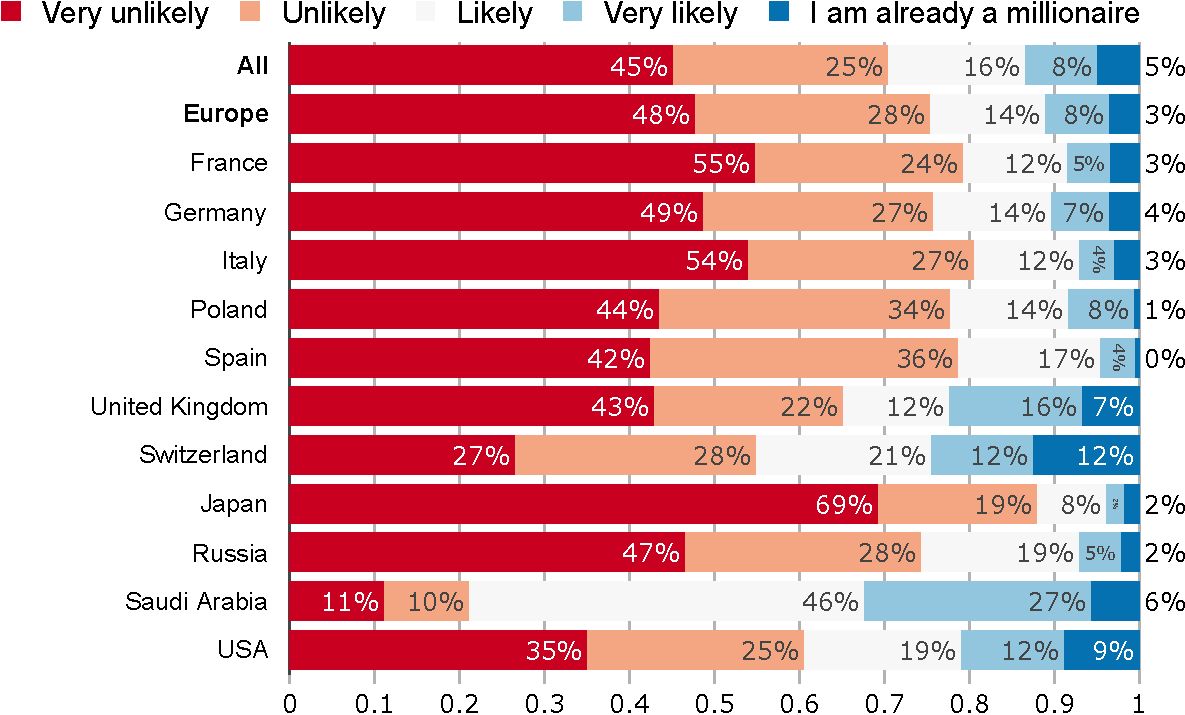
\includegraphics[width=.8\textwidth]{../figures/country_comparison/millionaire_nolabel.pdf}} 
% \end{figure}

% \begin{figure}[h!]
%     \caption[Foreign origin]{``Were you or your parents born in a foreign country?'' (Question~\ref{q:foreign}).
%     }\label{fig:foreign}
%     \makebox[\textwidth][c]{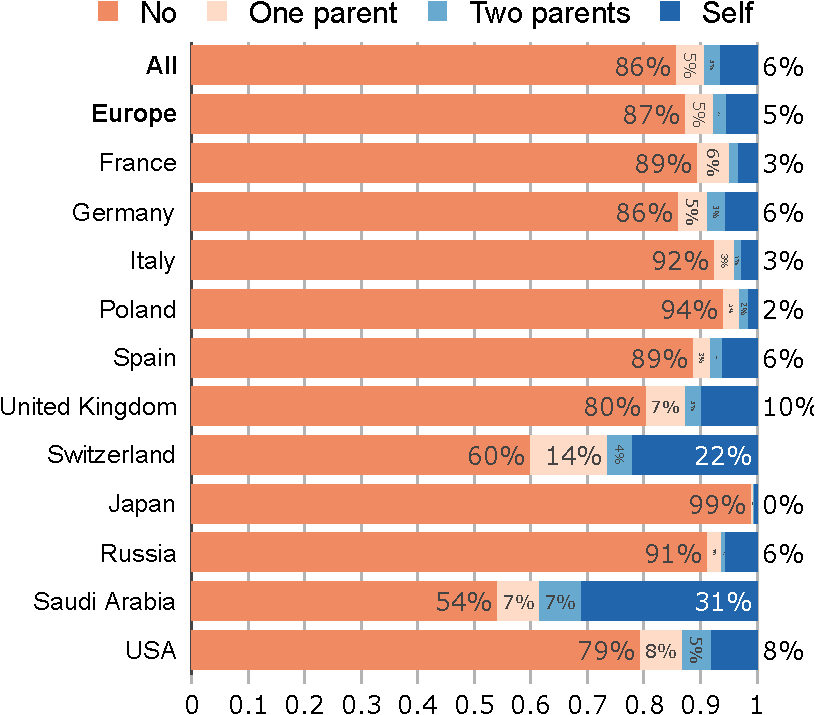
\includegraphics[width=.7\textwidth]{../figures/country_comparison/foreign_born_family_nolabel.pdf}} 
% \end{figure}

\begin{figure}[h!]
    \caption[Vote in the last election compared to actual results (among voters)]{Vote in the last election, compared to actual results among voters. (Questions~\ref{q:voted}, \ref{q:vote}). \hfill (Back~to~Section~\ref{par:representativeness}.)
    }\label{fig:vote_pnr_out}
    \makebox[\textwidth][c]{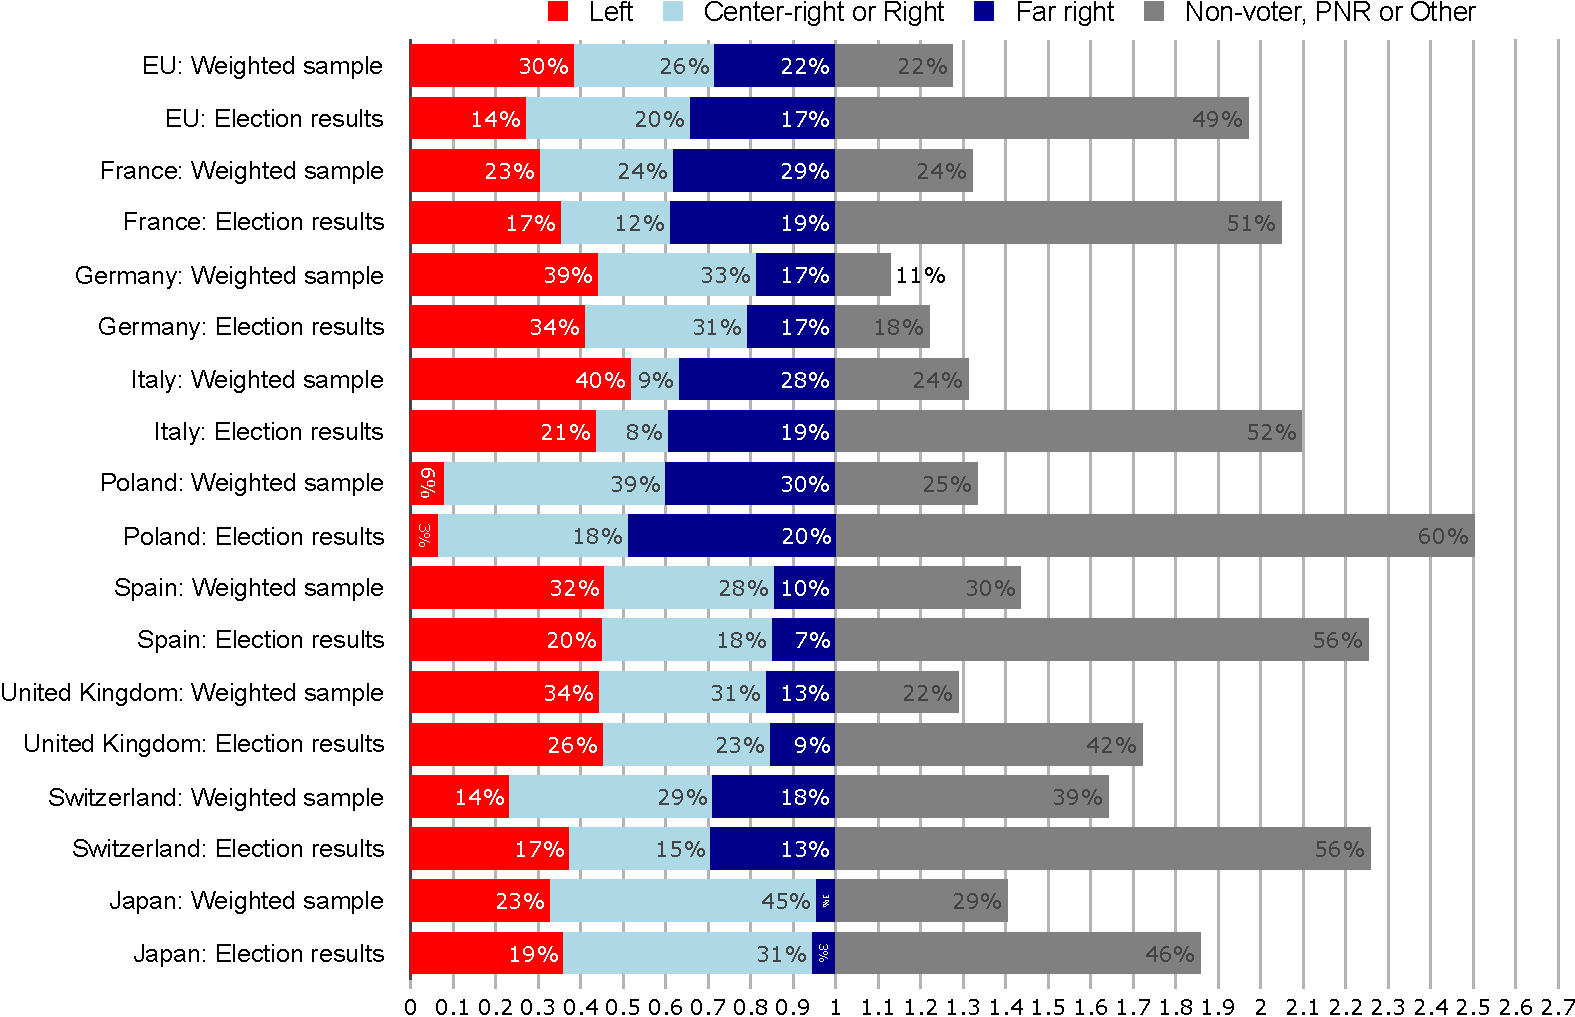
\includegraphics[width=\textwidth]{../figures/country_comparison/vote_pnr_out.pdf}} 
\end{figure}

% % \begin{figure}[h!]
% %     \caption[Vote in the last election compared to actual results (entire population)]{Vote in the last election, compared to actual results on the entire population. (Questions~\ref{q:voted}, \ref{q:vote}). \hfill (Back~to~Section~\ref{par:representativeness}.)
% %     }\label{fig:vote_representativeness}
% %     \makebox[\textwidth][c]{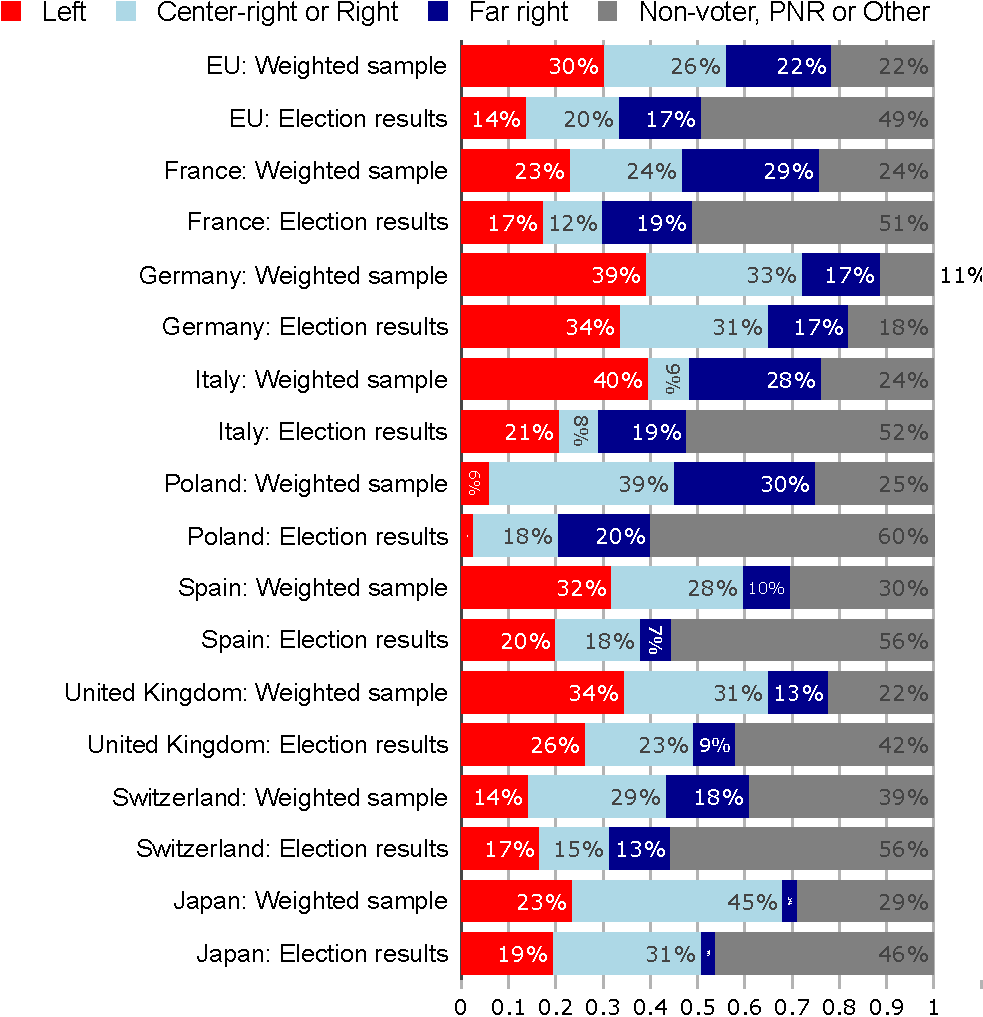
\includegraphics[width=.9\textwidth]{../figures/country_comparison/vote_representativeness.pdf}} 
% % \end{figure} % AER

% % \begin{figure}[h!]
% %     \caption[]{. (Question~\ref{q:gcs_support}).
% %     }\label{fig:gcs_support}
% %     \makebox[\textwidth][c]{\includegraphics[width=.9\textwidth]{../figures/country_comparison/gcs_support.pdf}} 
% % \end{figure}

% \clearpage
% \subsection{Countries' slant in the open-ended fields}\label{subsec:slant}
% % Interestingly, the topics vary significantly across countries. Below are my impressions of each country's slant. Compared to other countries, the concepts overrepresented 
% % in France are: insecurity, holidays or free time, the public deficit, equality, or gender equality; 
% % in Germany: old age poverty, immigration, the return of growth or the economic situation, free time, war (in Europe), and bureaucracy; 
% % in Italy: health, serenity or peace of mind, war, work stress and free time, world hunger, and femicides; 
% % in Poland: war, inequality, holidays, honesty, and disabled people; 
% % in Spain: ``health, money and love'', housing, corruption, water access, global poverty, and squatters; 
% % in the UK: the cost of living, immigration, having a comfortable life, mental health, the Holocaust, roads dangerous for driving, being unjustly imprisoned, and cuts to the winter fuel allowance; 
% % in Switzerland: equality, immigration, and gender equality; 
% % in Japan: the level of pensions, a cut to the consumption tax, the price of rice, the declining birth rate, childcare support, reducing the number of parliament members, foreigners' preferential treatment, excessive social assistance or the lack of reward for hard work, and stock prices; 
% % in Russia: metaphysical questions or profound interrogations, ``lies'', buying a house or a car, traveling, the desire to live; 
% % in Saudi Arabia: hobbies such as sports or soccer, the willingness to become millionaire (or billionaire), one's business project,\footnote{This can be linked to the high risk-taking disposition of Saudis \citep{falk_global_2018}.} buying a house, one's car, satisfaction with one's income, ``self-injustice'' or sin, raising children, Palestine, the oppression of orphans, and travel; 
% % in the U.S.: the economy, Donald Trump, breaches of the Constitution, abortion, and gun control. 
% Reading and coding each field one by one took about 30 hours. %, but it was worthwhile: not only does it result in an arguably more accurate classification; it also provides first-hand insight into how people think. 
% It gives first-hand insight on the topics vary significantly across countries. 
% Here are what I noted as %perceived / my impressions of 
% each country's unique topics. % slant. 
% Compared to other countries, the concepts overrepresented in each country are as follows:
% \begin{itemize}
%   \item France: insecurity, holidays or free time, the public deficit, equality, gender equality;
%   \item Germany: old age poverty, immigration, the return of growth or the economic situation, free time, war (in Europe), bureaucracy;
%   \item Italy: health, serenity or peace of mind, war, work stress and free time, world hunger, femicides; 
%   \item Poland: war, inequality, holidays, honesty, disabled people;
%   \item Spain: ``health, money and love'', housing, corruption, water access, global poverty, squatters;
%   \item the UK: the cost of living, immigration, having a comfortable life, mental health, the Holocaust, roads dangerous for driving, being unjustly imprisoned, cut to the winter fuel allowance;
%   \item Switzerland: equality, immigration, gender equality;
%   \item Japan: the level of pensions, a cut on the consumption tax, the price of rice, the declining birth rate, childcare support, reducing the number of parliament members, foreigners' preferential treatment, excessive social assistance or the lack of reward for hard work, stock prices;
%   \item Russia: metaphysical questions or profound interrogations, ``lies'', buying a house or a car, traveling, the desire to live;
%   \item Saudi Arabia: hobbies such as sports or soccer, the willingness to become millionaire (or billionaire), one's business project,\footnote{This can be linked to the high risk-taking disposition of Saudis \citep{falk_global_2018}.} buying a house, one's car, satisfaction with one's income, ``self-injustice'' or sin, raising children, Palestine, the oppression of orphans, travel;
%   \item the U.S.: the economy, Trump, breaches of the Constitution, abortion, gun control.
% \end{itemize}

% \renewcommand{\theenumi}{\arabic{enumi}}
% \clearpage
% \section{Questionnaire}\label{app:questionnaire}
% The U.S. version of the questionnaire is presented. Features that vary across countries are placed in square brackets within the question text, as follows: [feature\_name: U.S. value]. The features values for each country are provided in this spreadsheet [anonymized for review]. % APSR
% Random branches or conditions for displaying the question are specified in square brackets before the question text (cf. Figure \ref{fig:flow} for the survey flow). The question text is followed by square brackets that refer to Sections, Figures, and Tables presenting the question results, and the variable name(s) corresponding to the question. Finally, response options are displayed in italics. 
% Unless otherwise specified, responses are compulsory and a single response much be chosen. \hfill (Back~to~Section~\ref{par:flow}.)

% \input{app_questionnaire_AJPS}

% \clearpage
% \section{Survey Sources and Features}\label{app:features}

% \subsection{Sources Regarding Plausible Global Policies}\label{subsec:plausible_policies_sources}

% % \paragraph{Plausible global policies.} 
% Table \ref{tab:plausible_policies} provides references showing that the ``plausible global policies'' I test (Section~\ref{subsec:debated}) are (similar to proposals) debated in international negotiations.

% \begin{table}[H]
% \caption[Sources for plausible global policies]{Proposals similar to the ``plausible global policies'' in international negotiations.}
% \label{tab:plausible_policies}
% \begin{tabular}{p{5cm}p{11cm}}
% \toprule
% Proposal & Appearance in international negotiations and source \\
% \midrule
% A minimum tax of 2\% on the wealth of billionaires, in voluntary countries  & Proposal by \cite{zucman_blueprint_2024} in a report commissioned by the Brazilian presidency of the G20. \\ \addlinespace 
% Raising the globally agreed minimum tax rate on profits of multinational firms from 15\% to 35\%, closing loopholes and allocating revenues to countries where sales are made  & In the context of OECD/G20 discussions to address Base Erosion and Profit Shifting (BEPS), a similar proposal has been proposed by the Independent Commission for the Reform of International Corporate Taxation \citep{icrict_icrict_2020}: taxing coporate income through formulary apportionment at a 25\% rate. \\ \addlinespace 
% Expanding the UN Security Council (in charge of peacekeeping) to new permanent members such as India, Brazil, and the African Union, and restricting the use of the veto  & The Pact for the Future was adopted by the UN General Assembly. It includes ``Action 39. We will reform the Security Council, recognizing the urgent need to make it more representative, inclusive, transparent, efficient, effective, democratic and accountable (...) we agree on the following guiding (...) Enlarge the Security Council (...) increase representation of developing countries (...) The question of the veto is a key element of Security Council reform. We will intensify efforts to reach an agreement on the future of the veto, including discussions on limiting its scope and use'' \citep{un_pact_2024}.  \\ \addlinespace 
% Developed countries contributing at least 0.7\% of their GDP in foreign aid and development assistance  & This commitment has been made at the UN in 1971 and renewed ever since, e.g. in the SDG 17.2 \citep{unga_declaration_1971,un_sustainable_2017}. In 2024, developed countries contributed 0.33\% of their GNI in Official Development Assistance \citep{oecd_preliminary_2025}. \\ 

% \end{tabular}
% \end{table}
% \begin{table}[H]
% \caption*{(continued)}
% \begin{tabular}{p{5cm}p{11cm}}
% Debt relief for vulnerable countries by suspending repayments until they are better able to repay, promoting their development  & At the Financing for Development conference, all countries (except the U.S.) have ``recognize[d] the need to assist developing countries in attaining long-term debt sustainability through coordinated policies aimed at fostering debt financing, debt relief, debt restructuring and sound debt management'' \citep{ffd4_outcome_2025}. \\ %Debt relief is the first demand of the Accra-Marrakech Agenda adopted by a group of 74 nations vulnerable to climate change, the \cite{v20_accra-marrakech_2023}. \\ \addlinespace 
% Institutions like the World Bank investing in many more sustainable projects in lower-income countries, and offering lower interest rates (the Bridgetown initiative)  & The \cite{bridgetown_initiative_bridgetown_2025} has been initiated by the government of Barbados and endorsed by the UN Secretary-General \citep{un_press_2023}. It includes different proposals, including the rechanneling and new issuance of Special Drawing Rights to recapitalize Multilateral Development Banks. \\ \addlinespace 
% Developed countries financing a fund to help vulnerable countries cope with loss and damage from climate change  & The COP27 ``decide[d] (...) to establish a fund for responding to loss and damage'' \citep{cop27_decision_2022}, to which \$768 million have been pledged as of \href{https://unfccc.int/event/pledges-to-the-fund-for-responding-to-loss-and-damage}{April 7, 2025}. \\ \addlinespace 
% Developed countries providing \$300 billion a year (0.4\% of their GDP) to finance climate action in developing countries  & COP29 adopted the NCQG and ``decide[d] to set a goal, (...) with developed country Parties taking the lead, of at least USD 300 billion per year by 2035 for developing country Parties for climate action'' \citep{unfccc_new_2024}. \\ \addlinespace 
% An international levy on carbon emissions from shipping, funding national budgets in proportion to population & The International Maritime Organization recently adopted a draft standard and feebate on carbon emissions from shipping \citep{imo_draft_2025}. While countries still have to agree on the allocation of the revenue, a \href{https://wwwcdn.imo.org/localresources/en/OurWork/Environment/Documents/Expert%20workshop/MEPC%2080-INF.39-Add.1%20-%20Report%20of%20the%20ad-hoc%20Expert%20Workshop%20on%20comparative%20analysisof%20candidate%20mid-term%20GHG%20redu...%20%28Secretariat%29.pdf}{group of contries} including China and Brazil proposed to allocate 30\% for developing countries; \href{https://wwwcdn.imo.org/localresources/en/OurWork/Environment/Documents/Expert%20workshop/Factsheets/GHG-EW%203-INF.2%20-%20Factsheet%20On%20Emission%20Cap-And-Trade%20System%20(Norway)%20(4).pdf}{Norway}  proposed to let the Green Climate Fund manage the revenue; and \href{https://wwwcdn.imo.org/localresources/en/OurWork/Environment/Documents/Expert%20workshop/Factsheets/GHG-EW%203-INF.4%20-%20Factsheet%20On%20Combination%20Of%20The%20Ghg%20Fuel%20Standard%20With%20A%20Levy%20(Denmark)%20(4).pdf}{Germany} that the revenue be used to ``strengthen the green transition, in particular in the SIDS and LDCs.'' \\ \addlinespace 
% An international levy on carbon emissions from aviation, raising ticket prices by 30\% and funding national budgets in proportion to population & While more narrow in scope, in 2025, a ``new aviation solidarity coalition on premium flyers (first- and business- class tickets, and private jets) has been launched by France, Kenya, Barbados, Spain, Somalia, Benin, Sierra Leone and Antigua \& Barbuda. It will be supported by the European Commission, and the \href{https://solidaritylevies.org/eight-countries-launch-solidarity-coalition-for-levies-on-premium-flyers/}{Global Solidarity Levies Task Force} (...) The coalition aims to improve domestic revenue mobilization of developing countries and support international solidarity.'' \\ \addlinespace 
% \bottomrule
% \end{tabular}
% \end{table}

% \subsection{Country-specific Features and Policies' Costs}\label{subsec:country_features}

% In the survey, various features are tailored to country-specific characteristics. 
% The workbook at [anonymized repository] contains all such features as well as their sources. % APSR
% In particular, it includes the following spreadsheets:
% \begin{itemize}
%     \item Quotas: targets for each category based on frequencies among the adult population, as well as their sources (namely official statistical agencies) and the definition of regions. The coding of regions and urbanicity is done in Qualtrics based on zip codes; with the zipcode correspondences exported in the repository folder [anonymized repository] using code in [anonymized repository]. % APSR
%     \item Income, income\_raw: brackets used in the income question (\ref{q:income}), and associated sources and computations. I use household-level income Russia and the U.S.; equal-split income for Saudi Arabia; and equivalised income (i.e. standard of living, accounting for family composition) for other countries. Data sources are Eurostat for EU countries, Rosstat for Russia, WID for Saudi Arabia, Census Bureau for the U.S., and LIS for the other countries. 
%     \item Policies, policies\_sources, policies\_leaning, policies\_party, policies\_leaning\_party: respectively the policies used in the conjoint experiment (Question~\ref{q:conjoint}), the source of each policy (i.e. the political program from which they come), their political leaning (classified manually as 0 if the policy is consistent only with a left-wing program, 2 for a right-wing one, and 1 otherwise), the party that proposed each policy, and their political leaning based on the party that proposed each policy.
%     \item Elections: results at the last election (used in Questions~\ref{q:voted}-\ref{q:vote}) including abstention share among citizens, as well as classifications of the parties: whether they are major (i.e. obtained more than 5\% of votes), and their political leaning (Left, Center-right or Right, Far right). 
%     \item Figures, features: country-specific figures used in the questionnaire, as detailed below.
% \end{itemize}

% % Below, I give an overview of the different features, as well as the methodologies used to compute the figures characterizing the questionnaire's policies. 

% Table \ref{tab:features} reports the figures used for each country for the National or Global Climate Scheme; the top income tax; and the revenue allocation of a wealth tax. Below, I detail the methodologies used for these and other questions. 

% \begin{table}[!h]
% \caption[Country-specific features]{\hypertarget{tab_features}{Country-specific features of the questionnaire}.}\label{tab:features}
% \makebox[\textwidth][c]{\input{../tables/features.tex}}
% \end{table}

% \paragraph{Climate Scheme.} 

% In the Climate Schemes, I assume a carbon price of \$95/tCO$_\text{2}$, corresponding to the price in 2025 for an emissions trajectory compatible with a global warming peaking at +1.8\textdegree{}C before 2100.\footnote{More precisely, I use the price trajectory of the integrated assessment model IMAGE in the scenario SSP2-2.6, as given by the \href{https://secure.iiasa.ac.at/web-apps/ene/SspDb/download/iam_v2/SSP_IAM_V2_201811.csv.zip}{IIASA}.} 
% After 2025, the decline in emissions is estimated to almost balance out the carbon price increase, in the sense that the GDP share of carbon pricing revenue would be roughly constant over the thirty years following the initial phase-in, before plummeting as net-zero approaches \citep{fabre_global_2024}. In other words, the cost of climate schemes provided to the respondents reflects the direct monetary costs expected from a carbon price aligned with the Paris Agreement.  

% In the National Climate Scheme, the average increase in expenditures is equal to the carbon price multiplied by the country's emissions per capita,\footnote{I use territorial CO$_\text{2}$ emissions from non-LULUCF by country from \cite{gutschow_country-resolved_2021}. I use the same source to estimate the emissions covered by the different scenarios in the International Climate Scheme.} and corresponds to the equal cash transfer each person would receive (Question~\ref{q:ncs_support}). Relative to the country's GDP per capita, this translates into the price increase reported in the Global Climate Scheme (GCS). To compute the amount lost, i.e. the net cost of the GCS for the average person in the country (Question~\ref{q:gcs_support}), I subtract the equal cash transfer from the increase in expenditures. 

% In case of a strictly equal per adult allocation of carbon price revenue, the global basic income would amount to \$45 per month, corresponding to the world average emissions multiplied by the carbon price. However, to prevent highly emitting middle-income countries from losing financially, the GCS departs from the egalitarian allocation by offering them a waiver from the mutualization of revenue, thereby lowering cash transfers in other countries \citep{fabre_plan_2024}. 
% When the country coverage is \textit{global}, as is implicitly the case in questionnaires for Russia, Saudi Arabia, and the U.S., this results in a global basic income of \$36 per month. 
% In European countries and Japan, the cash transfer is even lower, at \$22 per month, since I implicitly assume a \textit{high} country coverage (cf. Figure \ref{fig:ics_maps}) that excludes countries with the greatest emissions per capita. 
% As I conservatively use low figures for the cash transfer, the GCS question could somewhat underestimate acceptance of a global, egalitarian cap-and-trade in high-income countries. 

% % In the International Climate Schemes, the question implicitly assumes that the costs would be the same as in the generic GCS question. This is credible if one assumes that each country would benefit for the same emissions rights in both cases. Indeed, as country coverage shrinks, two effects approximately balance out: the lower carbon price and the lower basic income, both of which result from lower emissions per capita within the climate coalition compared to the world average.

% \paragraph{Global Income Distribution.}

% To estimate the global income distribution, I use the distributions of disposable income by country in 2019 constructed by \cite{fisher-post_government_2023} (FPG).\footnote{The data is available on Amory Gethin's \href{https://www.dropbox.com/scl/fi/rd1d7rke0wwwr6948ea67/fisher-gethin-redistribution-2025-01-10.dta}{website}.} I inflate all generalized percentiles by real GDP growth observed between 2019 and 2024 (using IMF data), factor in country-specific inflation until 2022 and convert values from LCU to 2022 PPP dollars (using FPG), and finally assume that all countries experienced the same inflation as in the U.S. in 2023 and 2024 (using IMF data). 

% To aggregate country distributions, I compute the global cumulative distribution function and interpolate it at each thousandile. I obtain the global distribution of disposable income at purchasing power parity (PPP) in 2024. 

% I use this distribution for the custom redistribution task, after converting back to LCU (Section~\ref{subsec:custom_redistr}, Question~\ref{q:custom_redistr}). I also use it to calibrate the top income tax schedules so that they raise an amount equivalent to the poverty gap (Section~\ref{subsec:radical}, Questions~\ref{q:top1_tax_support}-\ref{q:top3_tax_support}). % top~1\% tax collects 2.1\% of global disposable income, matching the \$250 per month poverty gap; while the top~3\% tax collects 5.1\% of global income, corresponding to the \$400 per month poverty gap. 
% Then, I use country-level data to estimate the share of GDP collected as well as the share of the population affected by each tax in each country. 
% Finally, I compute the poverty gaps and the tax revenue in every country in proportion to GDP, and aggregate them at the global level after converting national disposable income back to market exchange rates (using World Bank's PPP conversion factors for 2022). 
% I find that the top~1\% tax collects 1.8\% of global nominal income, while the top~3\% tax collects 4.8\% of global nominal income. These amounts are higher than the respective poverty gaps: 1.3\% of global nominal income for a \$250 per month poverty line, and 3.2\% for a \$400 per month poverty line. 
% While the cost of poverty reduction declines relative to tax revenue once one accounts  for market exchange rates, closing the poverty gap actually requires extra revenue due to imperfect targeting and administrative costs \citep{sahoo_what_2025}. Therefore, the tax schedule calibrations are consistent with the poverty reduction objectives.

% \paragraph{Wealth Tax Revenue.}

% To estimate the revenue from a global tax on wealth above \$5 million at a rate of 2\% (Section~\ref{subsec:revenue_split}, Questions~\ref{q:revenue_split_few}-\ref{q:revenue_split_many}), I use the distribution of net wealth by country in current dollar for 2022 from the World Inequality Database. I assume that the taxable base is reduced by 30\% due to tax avoidance and asset depreciation. I report expected tax revenue as a share of countries' 2023 GNI (from the World Bank). I also report the absolute revenue after converting them into LCU. 

% \paragraph{Sustainable future; aviation levy.}

% I assume a carbon price of \$300/tCO$_\text{2}$. Given natural gas footprint at .1807 tCO$_\text{2}$/MWh, this carbon price would double a gas price of \$54/MWh, which is a midpoint between U.S. and European prices. Similarly, the prices of beef and flights would double, assuming that beef costs \$10/kg and emits 33~kgCO$_\text{2}$e/kg, and aviation emits 3~kgCO$_\text{2}$e per dollar of flight. A 30\% increase in flight prices corresponds to a carbon price of \$100/tCO$_\text{2}$, or to a \$300/t levy which does not account for the warming effect of contrails \citep{lee_contribution_2021}.
% %flights prices would raise by 30\%. 
% % Approximating emissions from aviation at 1~kgCO$_\text{2}$ per dollar of flight, a carbon price of \$300/tCO$_\text{2}$ would raise flights prices by 30\%. Similarly, assuming a (low) price of beef of \$10/kg and emissions of 33~kgCO$_\text{2}$e/kg. 

% % increased the price of beef by 75%, heating fuel or gas by 40%, and air travel by 30 => doubled the price of beef, heating fuel or gas, and air travel.
% % 1-5 kgCO2 per kg beef (Lynch & Pierrehumbert, 2019). Beef cost $11-22/kg in U.S. => Price of $200-400/t -> price +2-10%
% % 30-44 kgCO2eq per kg. => Price on all GHG of $200 (for $11/kg) to 400 (for $22/kg) => price +75% 
% % Decomposition is methane: ~50%, N2O: ~40%, CO2: ~10%.
% % Chicken/pork/eggs: +20%; coffe/chocolate: +40%
% % Flight: 1 kgCO2 per $ => $200-400/t -> price +20-40%
% % Natural gas: .0053 tCO2/therm * .0341 therm/kWh = .1807 tCO2/MWh => $300/t -> price +$54/MWh https://www.epa.gov/energy/greenhouse-gas-equivalencies-calculator-calculations-and-references https://www.unitjuggler.com/convertir-energy-de-kWh-en-thm.html 
% % Current natural gas price for EU consumer: €110/MWh (pre-crisis: €70). https://ec.europa.eu/eurostat/statistics-explained/index.php?title=Natural_gas_price_statistics
% % Similar price / price increases for heating fuel https://www.insee.fr/en/statistiques/serie/000442573
% % Current natural gas price for EU consumer: $53/MWh https://www.eia.gov/dnav/ng/hist/n3010us3a.htm https://www.kylesconverter.com/energy,-work,-and-heat/cubic-feet-of-natural-gas-to-megawatt-hours

% \paragraph{NCQG.} 

% The sources used for the New Collective Quantified goal of climate finance for 2035 (Section~\ref{subsec:debated}, Questions~\ref{q:ncqg_full}-\ref{q:ncqg}) are the following: \cite{unfccc_new_2024} states the goal itself, \cite{oecd_climate_2024} provides figures on past achievements, \cite{earth_negotiations_bulletin_daily_2024} reports the positions of India and other countries, and \cite{climate_action_network_climate_2024,demand_climate_justice_engo-demand_2025} those of NGOs. Note that the question wordings do not mention the gap between climate finance needs and the official goal identified in official reports \citep{oecd_bridging_2024,songwe_raising_2024}, nor that existing plans by Multilateral Development Banks (MDBs) to ramp up climate finance would achieve most of the new goal \citep{mdbs_joint_2024}.\footnote{According to the  \cite{oecd_climate_2024}, MDBs contributed \$81~billion to climate finance in 2022 (both directly through finance provision and indirectly through mobilization of the private sector), with 71\% (or \$58 billion) attributable to developed countries. Before the NCQG was agreed at COP29, they jointly stated that they will contribute an estimated \$185 billion in 2030 (including \$65 billion from the private sector). Assuming that this increase of \$104 billion is replicated in the period 2030-2035, MDBs would contribute \$289 billion in 2035, including \$205 attributable to developed countries, that is \$147 billion more than in 2022. As (multilateral plus unilateral) developed countries' climate finance totaled \$116 billion in 2024, adding the \$147 billion expected in their multilateral finance would achieve three-quarter of the required increase, at \$263 billion.}

% To express the NCQG as a share of developed countries' GDP, I use 2024 data from the World Bank on nominal GDP in high-income countries. This figure ---of \$70 trillion--- is conservative, since it does not account for growth or inflation until 2035.
% % Actually I accounted for growth, but used a weird source underestimating developed countries' GDP:
% % GDP advanced: 61.35T / others: 43.44 in 2023: IMF (https://www.statista.com/statistics/256328/gross-domestic-product-gdp-of-selected-global-regions/); Growth per year by 2035 advanced: 1.59% / all: 2.7% (https://www.spglobal.com/en/research-insights/special-reports/look-forward/emerging-markets-a-decisive-decade) => GDP advanced 2035: 61.35*1.0159^12=74.1T / others: world-74=(61.35+43.44)*1.027^12=144-74=70T, i.e. 51% in advanced. NB: the difference between advanced and developed is South Korea, Singapore, Taiwan (Saudi Arabia and Slovenia are classified consistently using both definitions). I subtract 3.1 (South Korea, cf. spglobal above) + 0.9 (Taiwan, current GDP + 20%) + 0.6 (Singapore, current GDP + 20%) = 4.6T to obtain 69.5T for "developed" countries' nominal GDP in 2035.

% \subsection{Definition of Keywords}\label{subsec:keywords}

% Below are the keywords used to classify the open-ended fields on top-of-mind considerations (Figure \ref{fig:field_keyword}, Section \ref{subsec:considerations}, Questions~\ref{q:concerns_field}-\ref{q:issue_field}). The keyword search uses the R function \verb|grepl| and ignores case. The special character \verb|^| indicates the start of the string and \verb|$| the end. \hfill (Back~to~Section~\ref{subsec:considerations}.)
% \input{../tables/keywords.tex}
%  \hfill (Back~to~Section~\ref{subsec:considerations}.)

% Below are the keywords used to classify the open-ended fields. The keyword search uses R function \verb|grepl| with argument \verb|ignore.case = TRUE|. Special character \verb|\^{}| indicates the start of the string and \verb|$| the end.

% Here are keywords for top-of-mind considerations (Figure \ref{fig:field_keyword}, Section \ref{subsec:considerations}, Questions~\ref{q:concerns_field}-\ref{q:issue_field}): 
% \input{../tables/keywords.tex}

% Here are keywords for the end-of-survey comment field (Question~\ref{q:comment_field}): 
% \input{../tables/keywords_comment.tex}


% \subsection{Exploratory Factor Analysis}\label{subsec:efa}

% To construct a latent variable of support for global redistribution, I proceed in three steps. First, I standardize each variable of support by converting them into \textit{z}-scores, by subtracting the sample average and then dividing the result by the standard error. Both the mean and the standard error are computed using survey weights on the global sample. 
% Second, I run an exploratory factor analysis (EFA) with one factor, to obtain the \textit{loadings}, i.e. the weight of each variable in the latent factor (reported in Table~\ref{tab:efa}). 
% Third, I average all \textit{z}-scores, weighted by the loadings. 

% \begin{paracol}{2}
% \captionsetup{type=table} % treat next caption as a table caption
% \captionof{table}{Loadings from the Exploratory Factor Analysis}\label{tab:efa}
%         \input{../tables/efa.tex}       
% \end{paracol}
%  {\footnotesize \textit{Note}: Some variable names have been shortened: I shortened occurrences of \verb|help_lic| into \verb|why_hic_help_lic|, \verb|solidarity_support| into \verb|pl_support|, and \verb|expanding_security_council| into \verb|un_reform|. }

% ~\\
% The loading of a variable is similar to the average absolute correlation with the other support variables. Interestingly, the average absolute correlation of the latent indicator, at .54, is only marginally greater than that of \verb|share_solidarity_diff| (the difference between the shares of plausible policies supported and opposed), at .49, or that of the share of plausible policies supported, at .45. In other words, simple indicators based on the support or opposition to plausible policies capture attitudes towards global redistribution almost as well as a sophisticated latent variable. 

% I constructed another latent variable of support, using a full-information item factor analysis, based on multidimensional item response theory (MIRT). Unlike the EFA, MIRT does not assume that levels in a Likert-scale are spaced one unit apart; instead, it estimates parameters encoding the Likert scale that best account for latent support. The correlation between the two latent variables is extremely high (0.98). Therefore, although MIRT is a more accurate method, I use EFA because its results are more transparent to describe. \hfill (Back~to~Section~\ref{par:ranking}.) % Both latent variables share close average values in each subsample (by country or political leaning). 

\clearpage
\section{Representativeness of the Surveys}\label{app:representativeness}

\begin{table}[h!]
    \caption[Sample representativeness in All, Eu, EU]{Sample representativeness overall, in Europe, and in the European Union. %(Back to \ref{subsec:data}) 
    } \label{tab:representativeness_0}
    \makebox[\textwidth][c]{
        \resizebox*{!}{.73\textheight}{% 73 without notes cf. https://tex.stackexchange.com/questions/13809/resizing-a-table-by-textheight 
        \input{../tables/All_Eu_EU_bold.tex}
        }
    }
    {\footnotesize \textit{Note}: This table displays summary statistics of the samples alongside actual population frequencies. Bold cells denote frequencies beyond $\pm 20\%$ of population frequencies. 
    Detailed sources for each variable and country population frequencies, as well as the definitions of regions, diploma, urbanity, employment, and vote are available in this spreadsheet [anonymized for review]. \hfill (Back~to~Section~\ref{par:representativeness}.) % APSR
    } 
\end{table}

% \begin{table}[h!]
%     \caption[Sample representativeness in Eu, FR, DE, IT]{Sample representativeness in Europe, France, Germany, Italy. %(Back to \ref{subsec:data}) 
%     } \label{tab:representativeness_1}
%     \makebox[\textwidth][c]{
%         \resizebox*{!}{.60\textheight}{% 73 without notes cf. https://tex.stackexchange.com/questions/13809/resizing-a-table-by-textheight 
%         \input{../tables/Eu_FR_DE_IT_bold.tex}
%         }
%     }
%     {\footnotesize \textit{Note}: This table displays summary statistics of the samples alongside actual population frequencies. Bold cells denote frequencies beyond $\pm 20\%$ of population frequencies. 
%     Detailed sources for each variable and country population frequencies, as well as the definitions of regions, diploma, urbanity, employment, and vote are available in \this spreadsheet (available upon acceptance). 
%     } 
% \end{table}

\begin{table}[h!]
    \caption[Sample representativeness in FR, DE, IT]{Sample representativeness in France, Germany, Italy. %(Back to \ref{subsec:data}) 
    } \label{tab:representativeness_1}
    \makebox[\textwidth][c]{
        \resizebox*{!}{.60\textheight}{% 73 without notes cf. https://tex.stackexchange.com/questions/13809/resizing-a-table-by-textheight 
        \input{../tables/FR_DE_IT_bold}
        }
    }
    {\footnotesize \textit{Note}: This table displays summary statistics of the samples alongside actual population frequencies. Bold cells denote frequencies beyond $\pm 20\%$ of population frequencies. 
    Detailed sources for each variable and country population frequencies, as well as the definitions of regions, diploma, urbanity, employment, and vote are available in this spreadsheet [anonymized for review].  \hfill (Back~to~Section~\ref{par:representativeness}.) % APSR
    } 
\end{table}

\begin{table}[h!]
    \caption[Sample representativeness in PL, ES, GB, CH]{Sample representativeness in Poland, Spain, the UK, Switzerland. %(Back to \ref{subsec:data}) 
    } \label{tab:representativeness_2}
    \makebox[\textwidth][c]{\resizebox*{!}{.60\textheight}{\input{../tables/PL_ES_GB_CH_bold}}}
    {\footnotesize \textit{Note}: This table displays summary statistics of the samples alongside actual population frequencies. Bold cells denote frequencies beyond $\pm 20\%$ of population frequencies. 
    Detailed sources for each variable and country population frequencies, as well as the definitions of regions, diploma, urbanity, employment, and vote are available in this spreadsheet [anonymized for review].  \hfill (Back~to~Section~\ref{par:representativeness}.) % APSR
    } 
\end{table}

\begin{table}[h!]
    \caption[Sample representativeness in JP, RU, SA, US]{Sample representativeness in non-European countries. %(Back to \ref{subsec:data}) 
    } \label{tab:representativeness_3}
    \makebox[\textwidth][c]{\resizebox*{!}{.78\textheight}{\input{../tables/JP_RU_SA_US_bold}}}
    {\footnotesize \textit{Note}: This table displays summary statistics of the samples alongside actual population frequencies. Bold cells denote frequencies beyond $\pm 20\%$ of population frequencies. 
    Detailed sources for each variable and country population frequencies, as well as the definitions of regions, diploma, urbanity, employment, and vote are available in this spreadsheet [anonymized for review].  \hfill (Back~to~Section~\ref{par:representativeness}.) % APSR
    } 
\end{table}
\clearpage
\section{Determinants of Support}\label{app:determinants}


\begin{figure}[h!]
\caption[Variance decomposition]{Variance decomposition: share of the variance explained by each covariate (``Group defended when voting'' is present only in bottom subfigures.).}\label{fig:lmg}
\begin{subfigure}{.49\textwidth}
  \caption[]{Support for the Global Climate Scheme (10\% of the variable's variance is explained by this linear model). (Question~\ref{q:gcs_support})\label{fig:lmg_gcs}}
  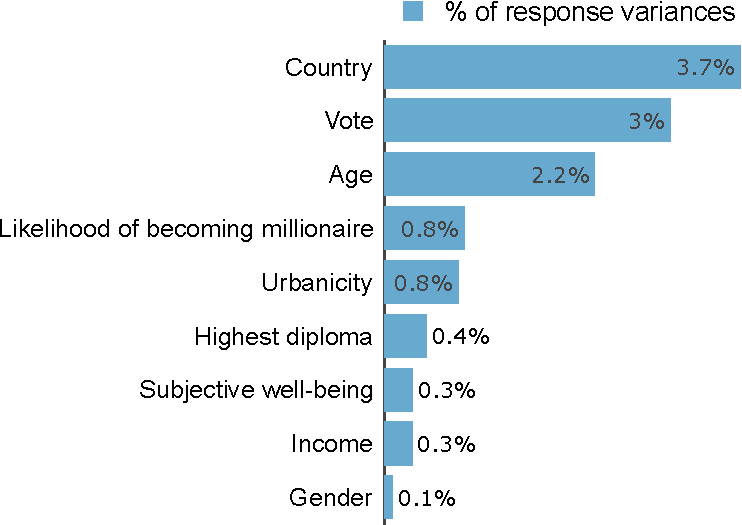
\includegraphics[width=\textwidth]{../figures/all/lmg_gcs_support_few.pdf}
\end{subfigure} \quad
\begin{subfigure}{.49\textwidth}
  \caption[]{Share of plausible global policies supported (15\% of the variable's variance is explained by this linear model). (Question~\ref{q:solidarity_support})\label{fig:lmg_solidarity}}
  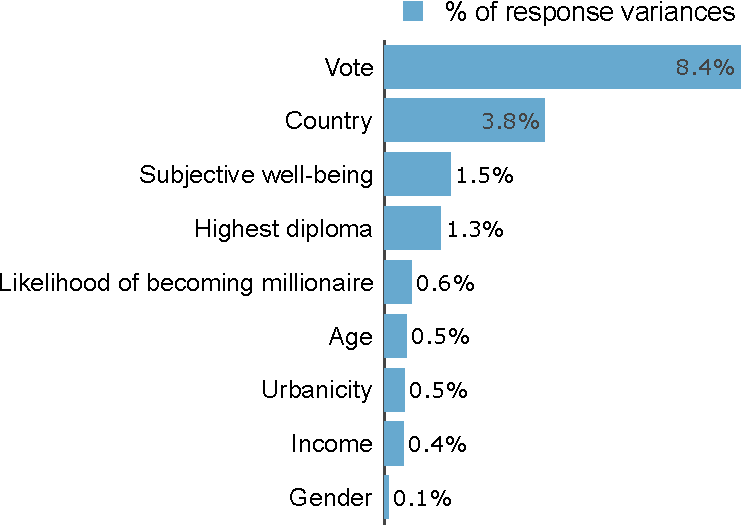
\includegraphics[width=\textwidth]{../figures/all/lmg_share_solidarity_supported_few.pdf}
\end{subfigure}

\vspace{.5cm}
\begin{subfigure}{.49\textwidth}
  \caption[]{Support for the Global Climate Scheme (14\% of the variable's variance is explained by this linear model). (Question~\ref{q:gcs_support})\label{fig:lmg_gcs_group}}
  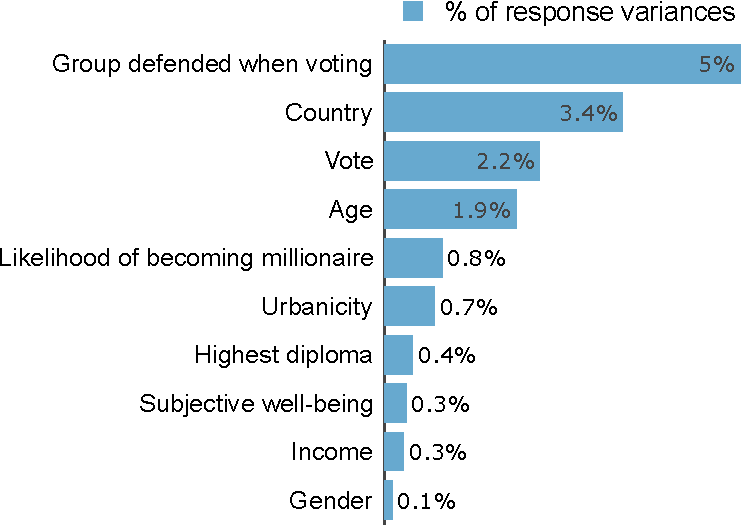
\includegraphics[width=\textwidth]{../figures/all/lmg_gcs_support_few_group.pdf}
\end{subfigure} \quad
\begin{subfigure}{.49\textwidth}
  \caption[]{Share of plausible global policies supported (20\% of the variable's variance is explained by this linear model). (Question~\ref{q:solidarity_support})\label{fig:lmg_solidarity_group}}
  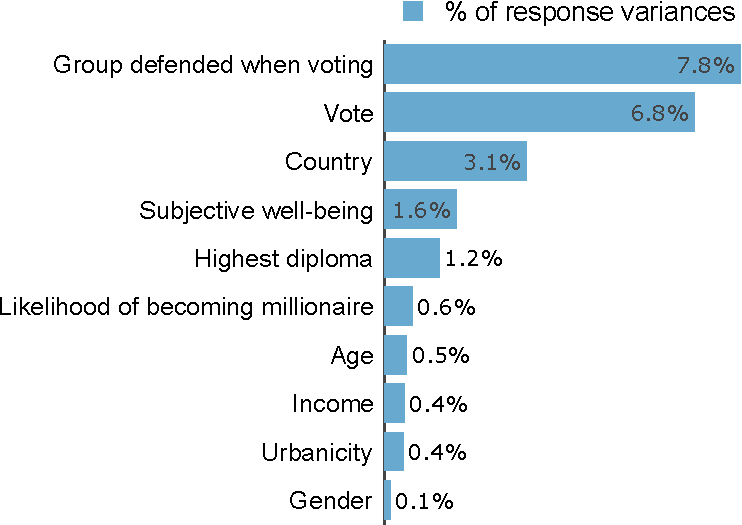
\includegraphics[width=\textwidth]{../figures/all/lmg_share_solidarity_supported_few_group.pdf}
\end{subfigure}
\end{figure}
% \hfill (Back~to~Section~\ref{par:representativeness}.)

\begin{table}[h]
    \caption[Correlates of support for global redistribution]{Correlates of support for global redistribution (multivariate OLS regressions). %(Back to \ref{subsec:gcs_stated_support})
    } \label{tab:determinant}
    \makebox[\textwidth][c]{
\resizebox*{!}{.73\textheight}{ % .67 if on same page as title
        \input{../tables/determinants_paper.tex}
        }
    }
    {\footnotesize \textit{Note}: Robust standard errors are reported in parentheses. Covariates omitted in the Table: \textit{Country}; \textit{Employment}; \textit{Couple}; \textit{Region}; \textit{Constant}. Omitted variables are: \textit{Vote: Non-voter, PNR or Other}; \textit{Gender: Woman}; \textit{Age: 35-49}; \textit{Income\_quartile: Q1}; \textit{Diploma: Below upper secondary}; \textit{Urbanicity: City}. \hfill $^{*}$p$<$0.1; $^{**}$p$<$0.05; $^{***}$p$<$0.01.
    }
\end{table}

% \begin{table}[h]
%     \caption[Correlates of answers on custom redistribution]{Correlates of answers on custom redistribution (multivariate OLS regressions). %(Back to \ref{subsec:gcs_stated_support})
%     } \label{tab:determinants_custom_redistr}
%     \makebox[\textwidth][c]{
% \resizebox*{!}{.73\textheight}{ % .67 if on same page as title
%         \input{../tables/determinants_custom_redistr.tex}
%         }
%     }
%     {\footnotesize \textit{Note}: Robust standard errors are reported in parentheses. Covariates omitted in the Table: \textit{Country}; \textit{Employment}; \textit{Couple}; \textit{Region}; \textit{Constant}. Omitted variables are: \textit{Vote: Non-voter, PNR or Other}; \textit{Gender: Woman}; \textit{Age: 35-49}; \textit{Income\_quartile: Q1}; \textit{Diploma: Below upper secondary}; \textit{Urbanicity: City}. \hfill $^{*}$p$<$0.1; $^{**}$p$<$0.05; $^{***}$p$<$0.01. 
    
%     \hfill (Back~to~Section~\ref{par:representativeness}.)
%     }
% \end{table}

% \clearpage
% \section{The Determination of a Custom Redistribution}\label{app:algo}

% In Question~\ref{q:custom_redistr}, respondents are asked for their preferred redistribution of the world's post-tax income. This custom redistribution is determined by modifying the current distribution using the respondent's three input parameters:\footnote{Overall, 35\% of the respondents did not move the sliders from their original position. Excluding the 39\% of them who still state that they are satisfied with the redistribution does not change the results qualitatively. Indeed, the average responses are similar between satisfied respondents who moved the sliders and all satisfied respondents: the shares of winners or losers, %differ by at most 2~p.p., 
% the implied minimum income or transfer %by less than 1\%, and the implied transfer by 
% all differ by less than 8\%. Therefore, I keep all satisfied respondents in the analysis. % mean_custom_redistr_stats
% }
% \begin{itemize}
%     \item The \textit{proportion of winners}, i.e. the share of people (at the bottom of the distribution) advantaged by the custom redistribution;
%     \item The \textit{proportion of losers}, i.e. the share of people (at the top) disadvantaged by the redistribution;
%     \item The \textit{degree of redistribution}, ranging from 0/10 (no redistribution) to 10/10 (maximal redistribution).
% \end{itemize}

% The determination of the custom distribution given these parameters relies on the algorithm \textit{Dis/adv} introduced by \cite{fabre_french_2022}. In that paper, \cite{fabre_french_2022} surveyed two representative samples of French respondents. The first survey uncovered the median preferred parameters for a national income redistribution.\footnote{The median preferred proportions of winners and losers were 50\% and 10\%, respectively. The median preferred degree of redistribution was defined indirectly, using the median preferred demogrant: \euro{}800/month. The resulting redistribution entailed 12\% of GDP redistributed from the top 10\% to the bottom 50\%.} The second survey showed that 52\% supported the income redistribution defined using these parameters while only 26\% opposed it. Furthermore, a majority among the French respondents who expressed an opinion agreed that it is a good idea to ``determine the citizens' preferred tax schedule from a survey and then submit the proposal that would emerge from the survey to a referendum.'' Therefore, the algorithm \textit{Dis/adv} applied to median preferred parameters has been validated both through the support for the resulting redistribution and through the support for such democratic method of preference aggregation to determine an income redistribution. Nonetheless, the algorithm \textit{Dis/adv} is just a first attempt to adjust the tax schedule by aggregating citizens' preferences, and more appropriate methods may be proposed. Although \cite{fabre_french_2022} finds that the algorithm \textit{Dis/adv} fares better than another algorithm tested, the method still suffers from some limitations. In particular, the current method is difficult to understand for the users, and it only allows for redistribution from the rich to the poor (it would thus be inappropriate if the level of inequality were considered too low). Below, I describe the algorithm \textit{Dis/adv}, available for use at [anonymized for review], and implemented in the R function \verb|algo_dis_av| at [anonymized repository]. % APSR

% \paragraph{Algorithm Dis/Adv} 

% It is worth recalling that over a range of income (concerning people who are neither winner nor loser from the reform), both the current and custom distributions coincide. The algorithm proceeds as follows:

% \begin{figure}[b!]
%   \caption[Algorithm for the custom redistribution]{Algorithm for the custom redistribution, with parameters \textit{winners}: 60\%, \textit{losers}: 20\%, \textit{degree}: 4/10.} \label{fig:algo} 
%   \begin{subfigure}{.49\textwidth}
%     \caption[]{Steps 1 and 2.}
%     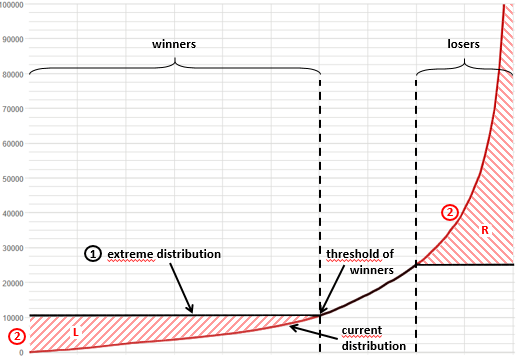
\includegraphics[width=\textwidth]{../figures/questionnaire/algo_1-2.PNG}
%   \end{subfigure} 
%   \begin{subfigure}{.49\textwidth}
%     \caption[]{Steps 3 and 4.}
%     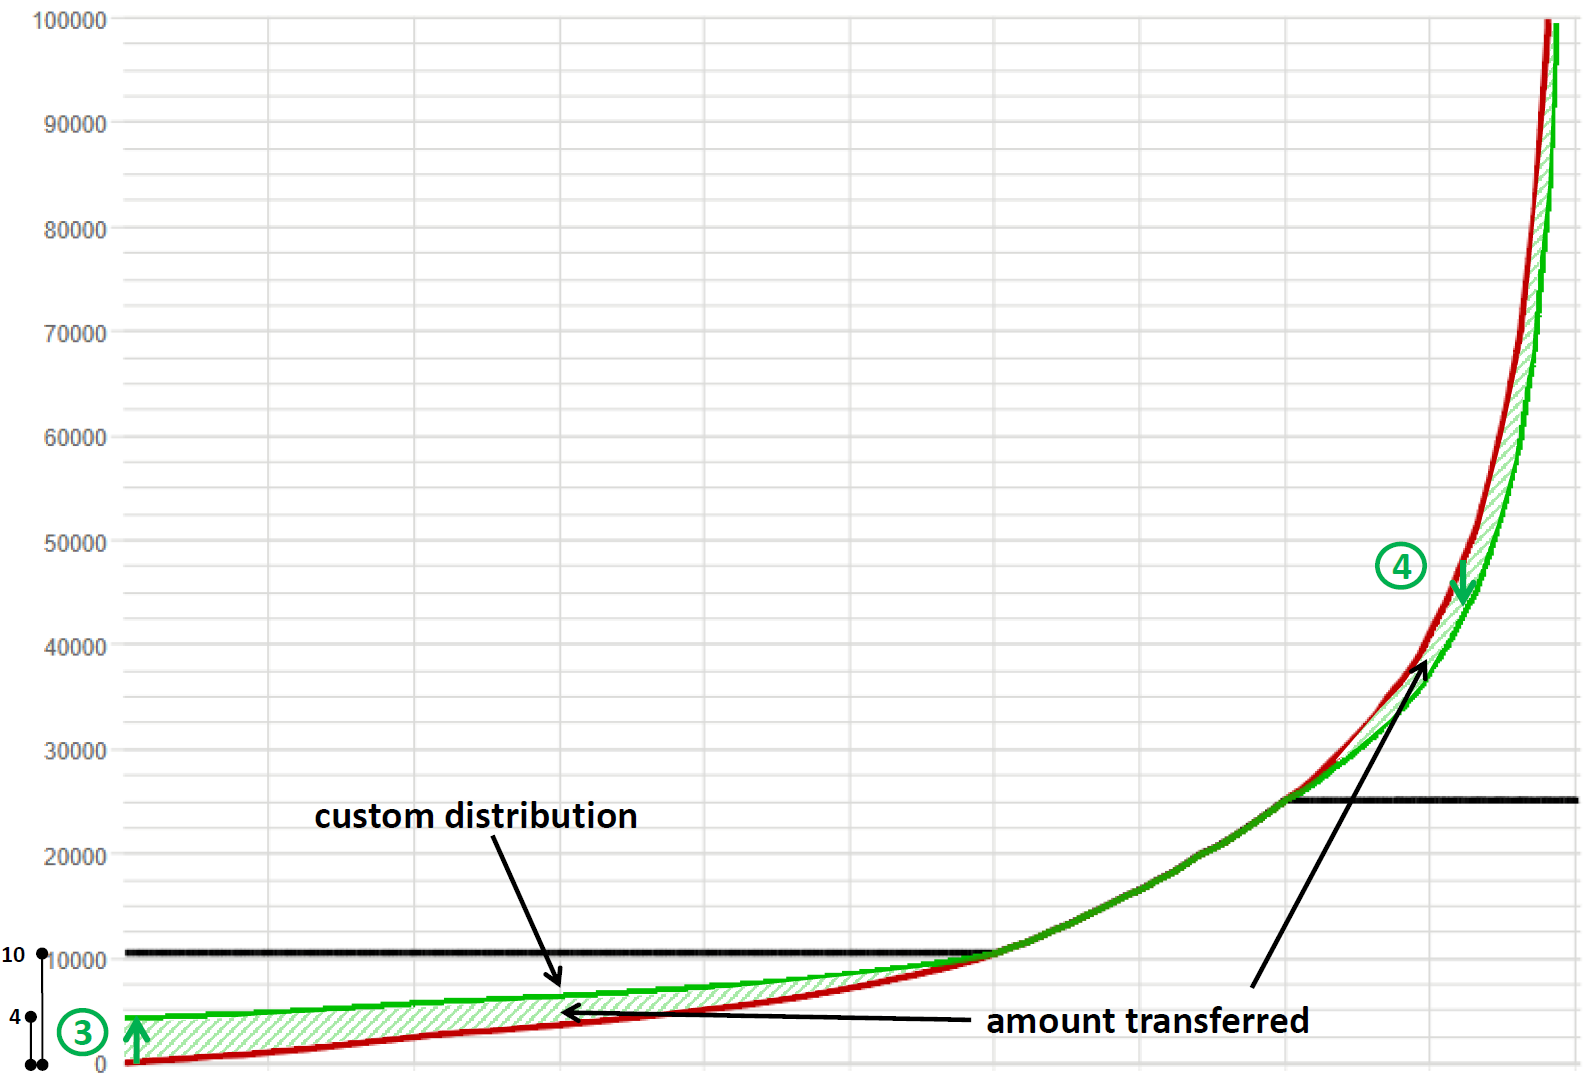
\includegraphics[width=\textwidth]{../figures/questionnaire/algo_3-4_full.PNG}
%   \end{subfigure}
% \end{figure}

% \begin{enumerate}
%     \item Define the \textit{extreme distribution} as the current distribution bounded by the income thresholds of winners and losers. In other words, draw two horizontal lines at each end of the distribution, by setting the incomes of winners to the income of the richest winner, and those of losers to the income of the poorest loser.
%     \item Compute what can be redistributed on either side as the area between the extreme and current distributions: what can be given to winners on the left side ($L$) or taken on the right side ($R$). If and only if what can be given is lower than what can be taken ($L < R$, as in Figure \ref{fig:algo}), the left side is binding, and it determines the \textit{amount transferred} from the rich to the poor: $\min\{L;\,R\} \cdot degree$.
%     \item On the binding side, define the custom distribution as a linear mixture between the current and extreme distributions, with the mixture parameter set by the \textit{degree of redistribution}. In other words, starting from the current distribution, narrow the gap with the extreme distribution by a factor \textit{degree}.
%     \item Adjust the non-binding side by narrowing the gap with the extreme distribution, using the unique mixture parameter that preserves aggregate income (so that the amount transferred is the same on both sides).\footnote{While we do not account for behavioral responses, one can adjust the algorithm to account for them. It suffices to define a post-reform aggregate income, which can be lower than the pre-reform one if the reform disincentivizes economic activity.}
%     \item ~[Optional step, used in the survey.] To increase the demogrant (i.e. the lowest income) and make the reform more progressive on the left side, try to replace the left side with a straight line. In other words, find the demogrant and the straight line between the demogrant and the threshold of winners that respects the amount transferred. If this straight line crosses the current distribution or if it implies a regressive redistribution (in that some incomes would increase less than higher incomes), abandon the straight line and keep the custom redistribution as is.
% \end{enumerate}

% Once the custom redistribution has been determined, it is straightforward to compute the additional tax schedule required to attain it.\footnote{For a sophisticated calculation of the required tax schedule, which allows for behavioral responses and a gradual implementation, see Appendix IX of \cite{fabre_french_2022}.} Figure \ref{fig:tax_radical_redistr} presents the tax schedule required to attain the average custom redistribution (weighted over all respondents). Figure \ref{fig:tax_radical_redistr} shows that (on the losers' side) this redistribution can ba approximated by additional marginal tax rates of 7\% above \$25,000 per year, and 16\% above \$40,000. Figure \ref{fig:tax_radical_redistr} also compares this tax schedule with those associated with the radical income redistribution tested in Questions~\ref{q:top1_tax_support}-\ref{q:top3_tax_support}: While the average custom redistribution features a much larger tax base than the radical tax targeting the top 3\% (as it taxes the top 28\%), its top tax rate is three times lower, so that the two redistributions entail similar transfers from the rich to the poor, at around 5\% of the world's income. % it features higher tax rates than the radical tax on the top 1\%, but 
% \hfill (Back~to~Section~\ref{subsec:custom_redistr}.)

% \begin{figure}[H]
%     \caption[Tax schedule of radical and custom redistributions]{Additional tax schedule associated with the radical and custom redistributions. (Questions~\ref{q:top1_tax_support}-\ref{q:top3_tax_support},~\ref{q:custom_redistr}).
%     }\label{fig:tax_radical_redistr}
%     \makebox[\textwidth][c]{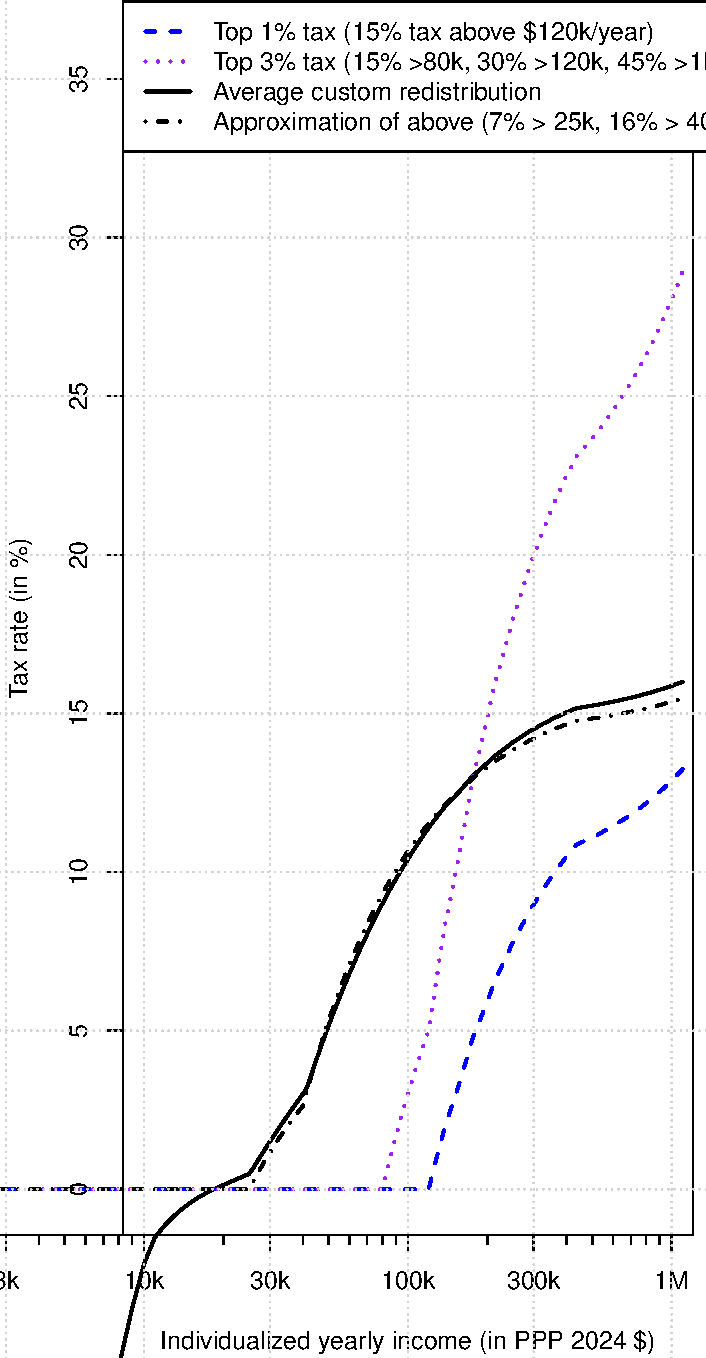
\includegraphics[width=.7\textwidth]{../figures/all/tax_radical_redistr.pdf}} 
% \end{figure}
%     \hfill (Back~to~Section~\ref{subsec:custom_redistr}.)

% % \clearpage % AER
% % \section{Comparison with Other Surveys}\label{app:comparison}
% % \begin{figure}[h!]
% % \caption[Comparison with other surveys]{Comparison with similar questions in other surveys.} \label{fig:comparison}
% % \begin{subfigure}{.45\textwidth}
% %   \caption[]{Absolute support for an international 2\% tax on billionaire wealth (cross-country correlation between this survey and \cite{cappelen_majority_2025}: .86). \hfill (Question~\ref{q:solidarity_support})}
% %   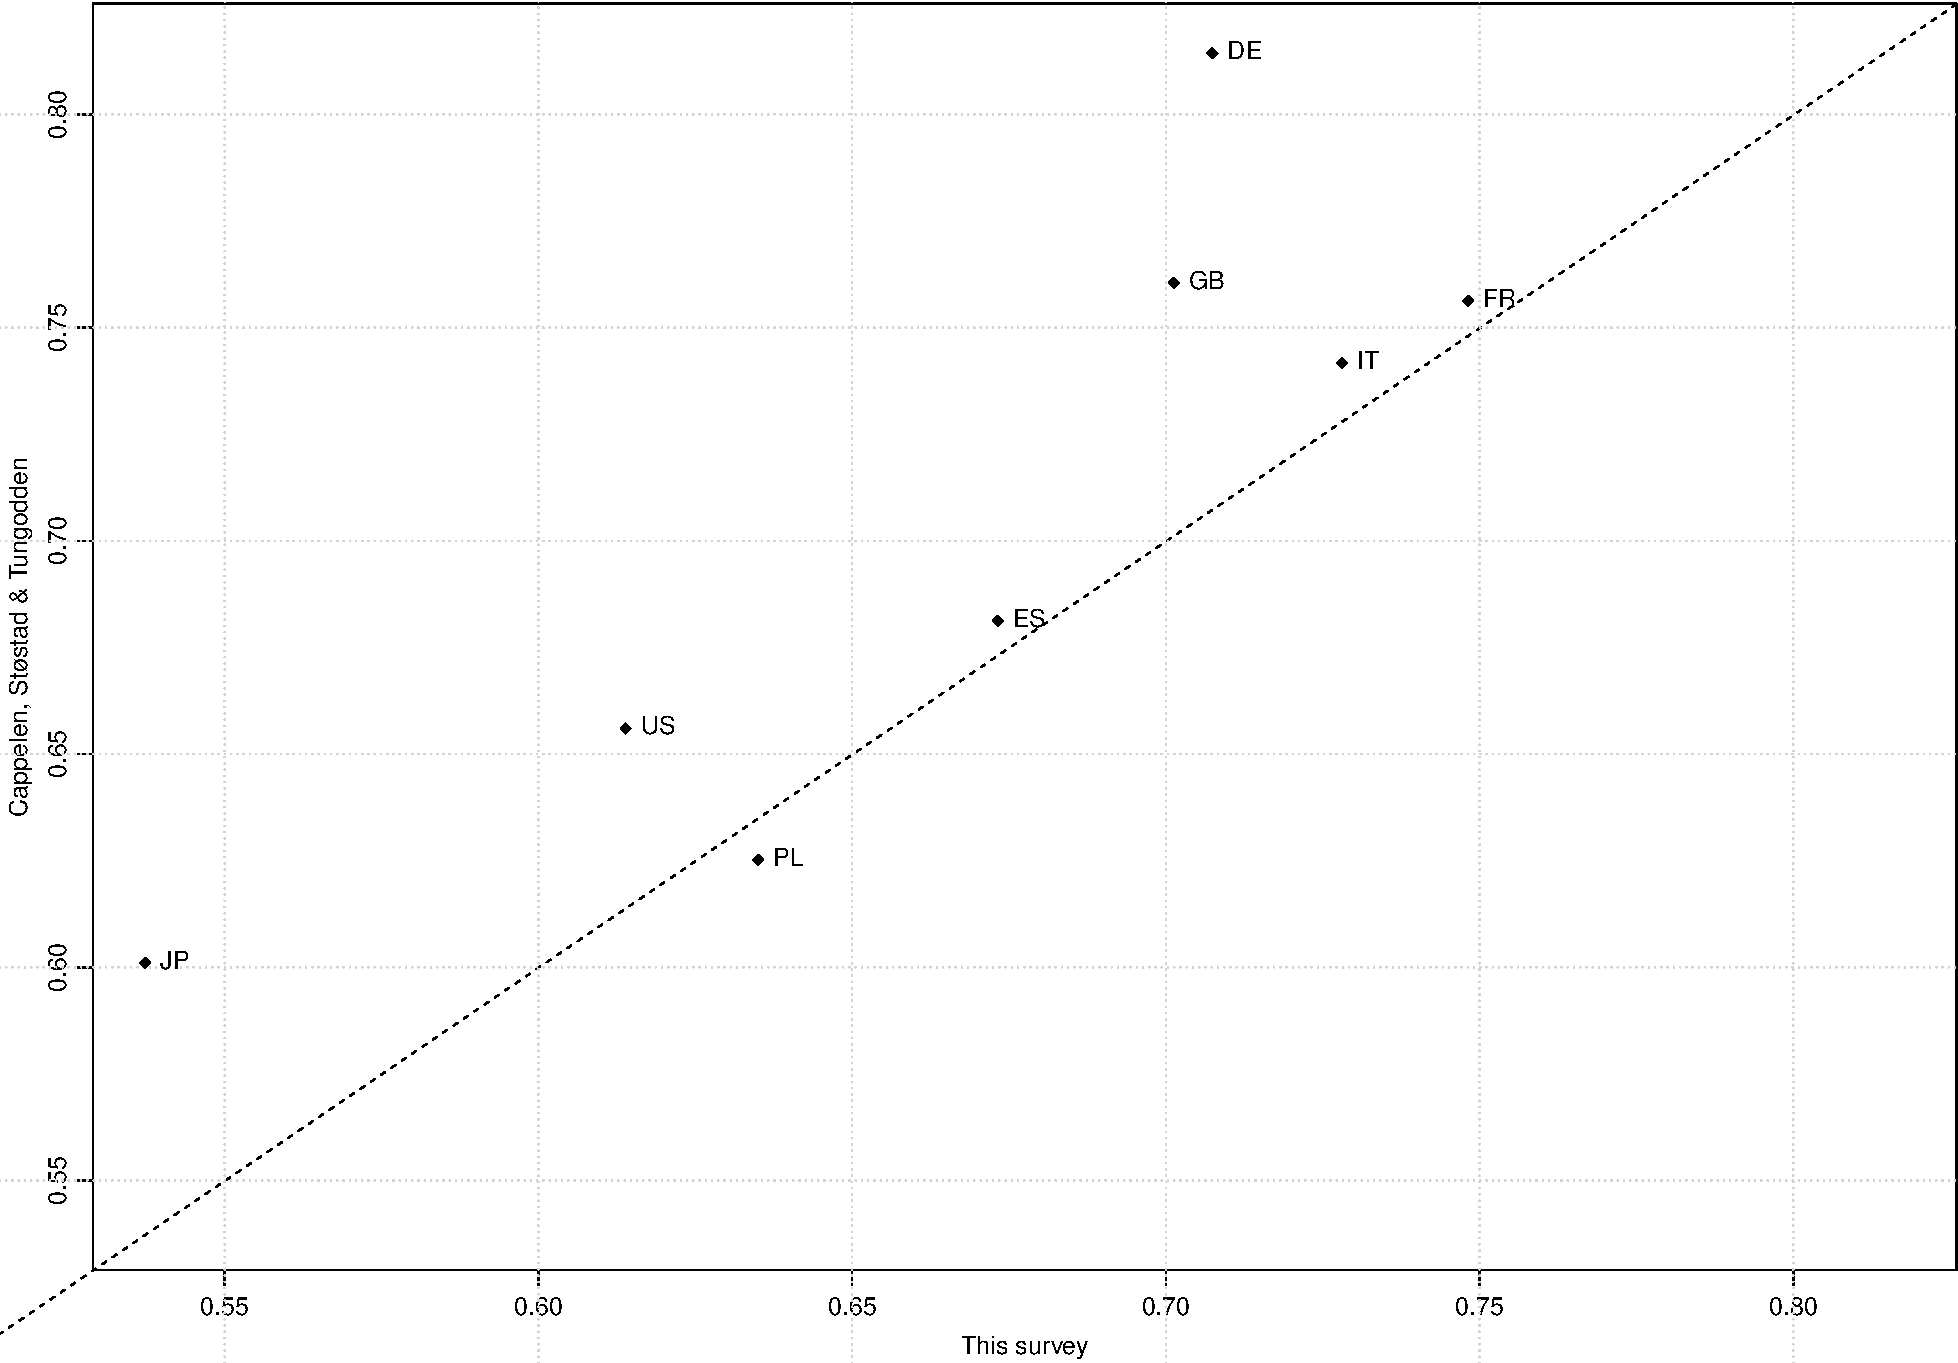
\includegraphics[width=\textwidth]{../figures/all/billionaire_stostad.pdf}
% % \end{subfigure} \quad
% % \begin{subfigure}{.45\textwidth}
% %   \caption[]{Relative agreement that ``My taxes should go towards solving global problems'' (cross-country correlation with \cite{global_nation_global_2023}: .70). \hfill (Question~\ref{q:my_tax_global_nation})}%\begin{flushright}
% %   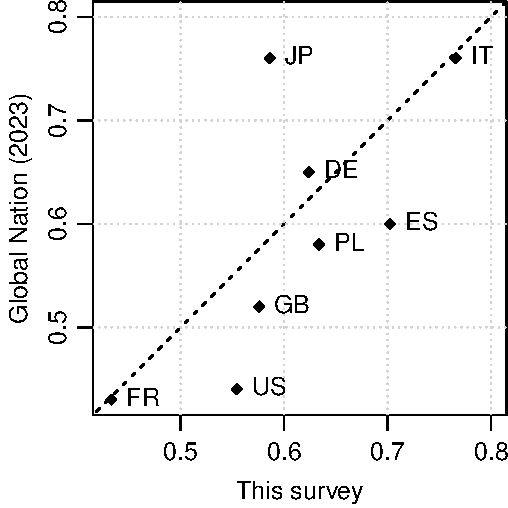
\includegraphics[width=\textwidth]{../figures/all/my_tax_global_nation_comparison.pdf}%\end{flushright}
% % \end{subfigure}
% % \end{figure}

\clearpage
\section{Attrition Analysis}\label{app:attrition}

\begin{table}[h!]
    \caption[Determinants of attrition]{sociodemographic determinants of attrition and exclusion. \hfill (Back~to~Section~\ref{par:data_quality}.)} \label{tab:attrition}
    \makebox[\textwidth][c]{\resizebox*{!}{.87\textheight}{ % 73 is the max when there is a title
        \input{../tables/attrition.tex}}}
    \centering {\footnotesize \textit{Note}: Robust standard errors are reported in parentheses. $^{*}$p$<$0.1; $^{**}$p$<$0.05; $^{***}$p$<$0.01.}
\end{table}

\begin{table}[h!]
    \caption[Treatment effects on attrition (1)]{Treatment effects on attrition. \hfill (Back~to~Section~\ref{par:data_quality}.)} \label{tab:attrition}
    \makebox[\textwidth][c]{\resizebox*{.98\paperwidth}{!}{ 
        \input{../tables/attrition_treatment.tex}}}
    \centering {\footnotesize \textit{Note}: Robust standard errors are reported in parentheses. $^{*}$p$<$0.1; $^{**}$p$<$0.05; $^{***}$p$<$0.01.}
\end{table}

\begin{table}[h!]
    \caption[Treatment effects on attrition (2)]{Treatment effects on attrition (continued). \hfill (Back~to~Section~\ref{par:data_quality}.)} \label{tab:attrition}
    \makebox[\textwidth][c]{\resizebox*{.98\paperwidth}{!}{
        \input{../tables/attrition_treatment2.tex}}}
    \centering {\footnotesize \textit{Note}: Robust standard errors are reported in parentheses. $^{*}$p$<$0.1; $^{**}$p$<$0.05; $^{***}$p$<$0.01.}
\end{table}

\clearpage
\section{Balance Analysis}\label{app:balance}

\begin{table}[h]
    \caption[Balance analysis]{Balance analysis.} \label{tab:balance}
    \makebox[\textwidth][c]{
\resizebox*{!}{.71\textheight}{ 
        \input{../tables/balance.tex}
        }
    }
    \centering {\footnotesize \textit{Note}: Robust standard errors are in parentheses. \textit{CS}: \textit{Climate Scheme}. $^{*}$p$<$0.1; $^{**}$p$<$0.05; $^{***}$p$<$0.01.
    }
\end{table}
\clearpage

\section{Placebo Tests}\label{app:placebo}



\begin{table}[!htbp] 
  \caption{Placebo tests of treatments on unrelated outcomes (simple OLS regressions).} \label{tab:placebo} 
  \makebox[\textwidth][c]{\input{../tables/placebo.tex}}
  Table \ref{tab:placebo} shows that in two cases (out of thirteen), treatments are significantly correlated with unrelated outcomes later in the survey, with an effect size up to 3~p.p. While these framing effects are undesirable, their magnitude is limited. Indeed, the average value of affected outcomes always remain within $\pm$2~p.p. of the value it is estimated to have had if any treatment had been generalized.\hfill (Back~to~Section~\ref{par:flow}.)
\end{table} 


\clearpage
\section{Main Results on Selected Demographics, Including Vote}\label{app:pol}

% Figures \ref{fig:main_radical_redistr_pol}--\ref{fig:synthetic_indicators_pol_mean} show that polarization between left- and right-wing voters is comparably high in Europe and the U.S. but almost non-existent in Japan, with Japanese support comparable to the support among non-voters in Western countries. Interestingly, although \cite{fabre_majority_2025} exhibited much higher polarization in the U.S. compared to Western Europe on similar questions (about the GCS, the globally redistributive millionaire tax, and universalism), in the current survey polarization has converged in the two regions. More specifically, compared to early 2023, in Western Europe (France, Germany, Spain and the UK), support has declined across the political spectrum, but more so among right-wing voters. Meanwhile, in the U.S., support has increased among Republican voters and decreased among Democrat voters. 
% % Polarization increased in Europe between Left and (Center+Far) Right since last paper (1-3/23): 14 -> 25 for GCS, 18 -> 26 for wealth_tax, 30 -> 32 for universalist. (Support for the three declined across categories but more so on the Right).
% % In the U.S. GCS: 48 -> 23, wealth_tax 45 -> 30, universalist: 30 -> 30 (Support stayed about the same in the Right (on average, depends on the policy) but declined on the Left)
% % Change in polarization could not be framing as GCS was asked the same in US and EU in each survey (but framing could explain change in level).

\begin{figure}[H]
    \caption[{[}On selected vote or nationality{]} Absolute support for global redistribution]{[On selected vote or nationality] Support for global redistribution action/policies. %\hfill (Questions \ref{q:gcs_support}, \ref{q:ics_support}, \ref{q:global_tax_support}-\ref{q:intl_tax_support}, \ref{q:sustainable_future}-\ref{q:top3_tax_support}, \ref{q:convergence_support}-\ref{q:vote_intl_coalition}, \ref{q:reparations_support}, \ref{q:my_tax_global_nation}).
    }\label{fig:main_radical_redistr_pol} 
    \makebox[\textwidth][c]{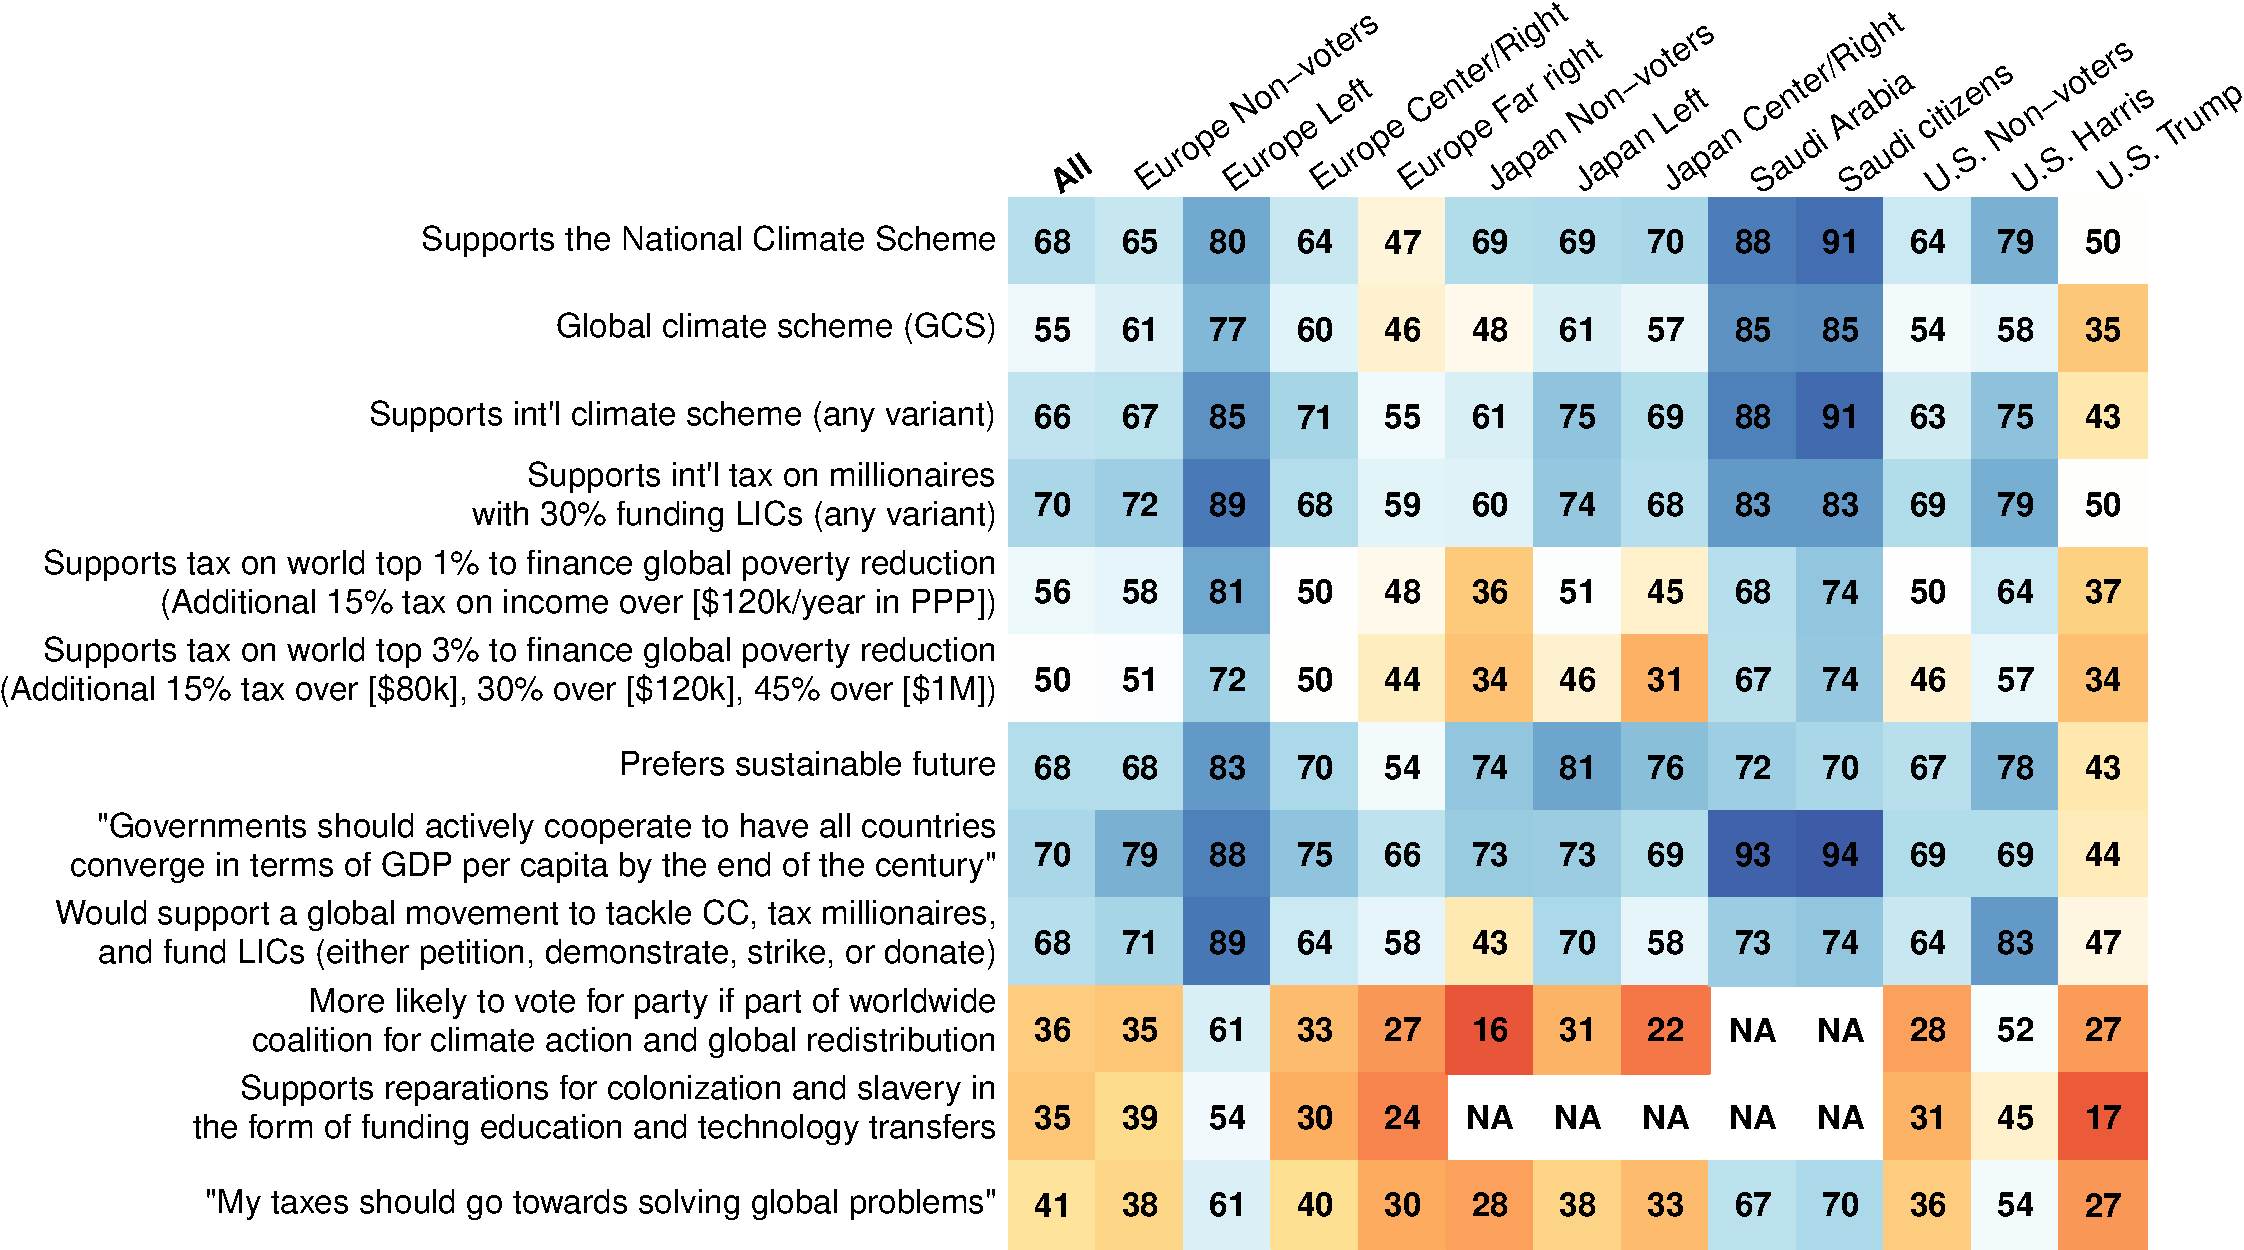
\includegraphics[width=\textwidth]{../figures/country_comparison/main_radical_redistr_pol_positive.pdf}} 
\end{figure}
\hfill (Back~to~Section~\ref{par:representativeness}.)

\begin{figure}[H]
    \caption[{[}On selected vote or nationality{]} Acceptance of plausible global policies]{[On selected vote or nationality] Acceptance of plausible global redistribution policies (Percentage of \textit{Somewhat} or \textit{Strongly support} among non-\textit{Indifferent} responses). %(Question~\ref{q:solidarity_support}).
    }\label{fig:solidarity_support_pol_share}
    \makebox[\textwidth][c]{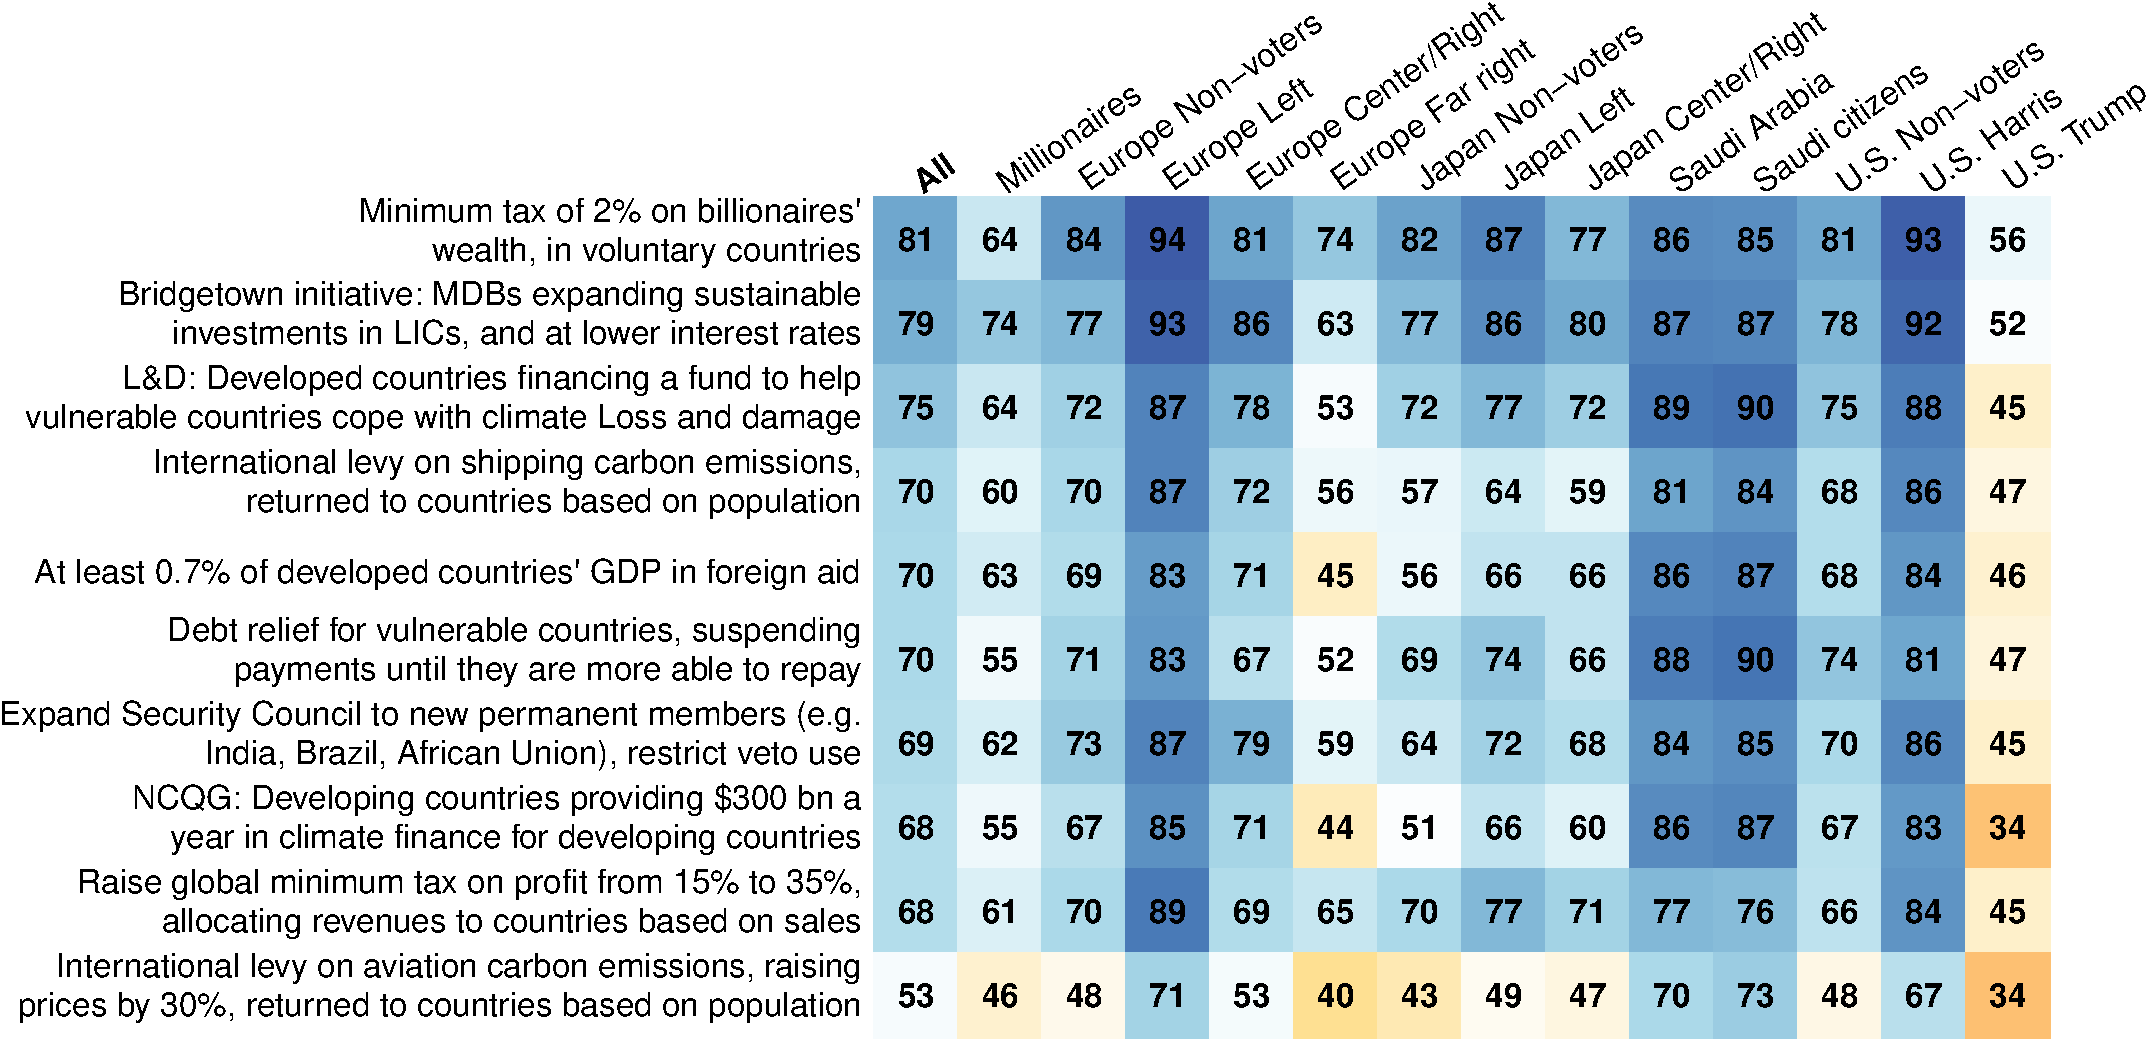
\includegraphics[width=\textwidth]{../figures/country_comparison/solidarity_support_pol_share.pdf}} 
\end{figure}

\begin{figure}[H]
    \caption[{[}On selected vote or nationality{]} Average synthetic indicators of support]{{[}On selected vote or nationality{]} Average synthetic indicators of support for global redistribution. (Question~\ref{q:solidarity_support}).  \hfill
    }\label{fig:synthetic_indicators_pol_mean}
    \makebox[\textwidth][c]{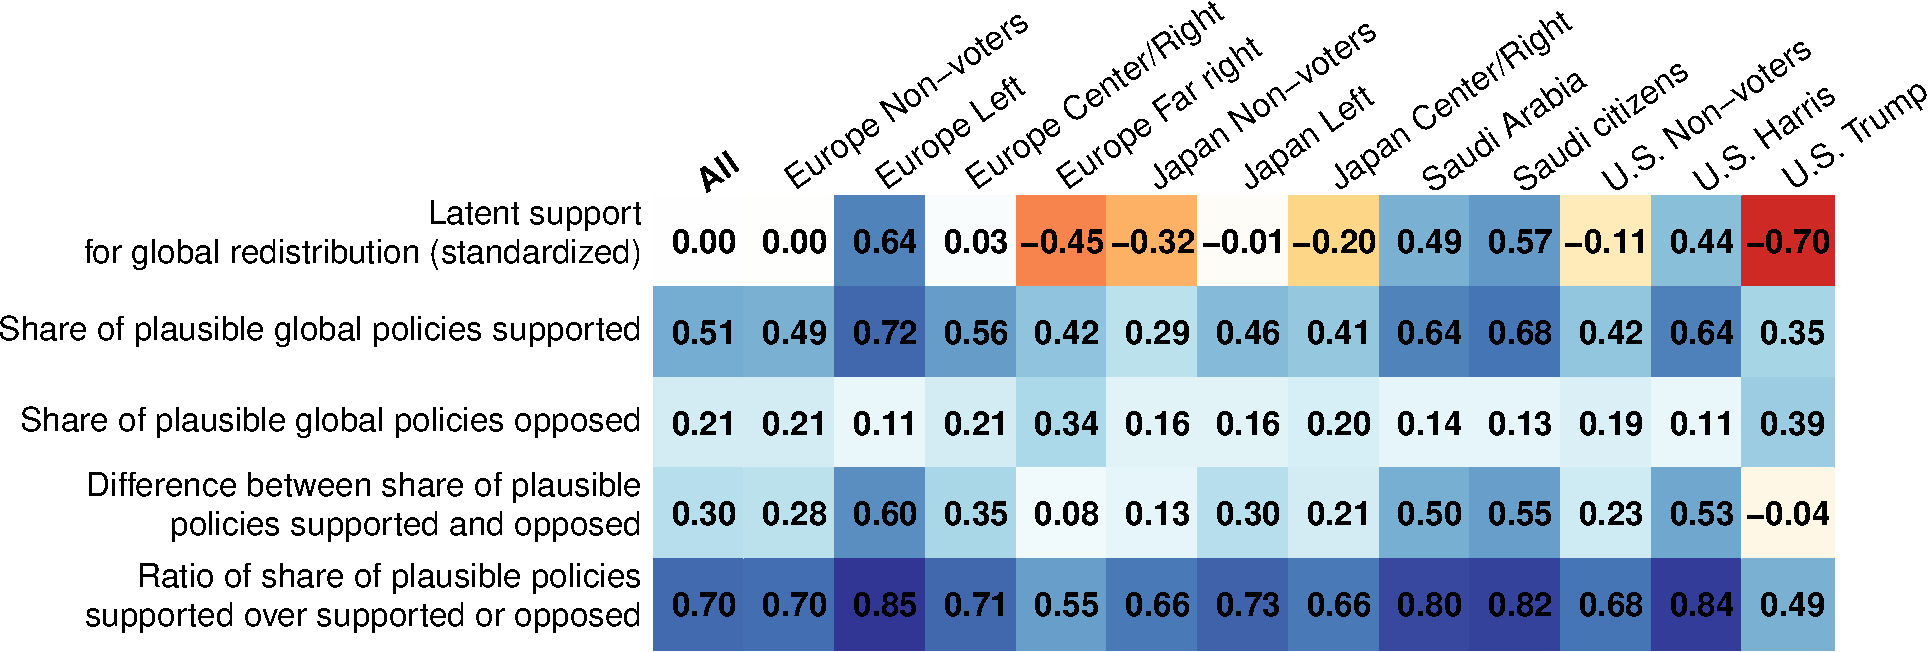
\includegraphics[width=\textwidth]{../figures/country_comparison/synthetic_indicators_pol_mean.pdf}} 
\end{figure}
% \hfill (Back~to~Section~\ref{par:representativeness}.)

% \begin{figure}[H]
%     \caption[{[}On selected vote or nationality{]} Manual classification of open-ended fields]{{[}On selected vote or nationality{]} Manual classification of open-ended fields. (Questions~\ref{q:concerns_field}-\ref{q:injustice_field}).\hfill (Back~to~Section~\ref{subsec:considerations}.)
%     }\label{fig:field_manual_pol}
%     \makebox[\textwidth][c]{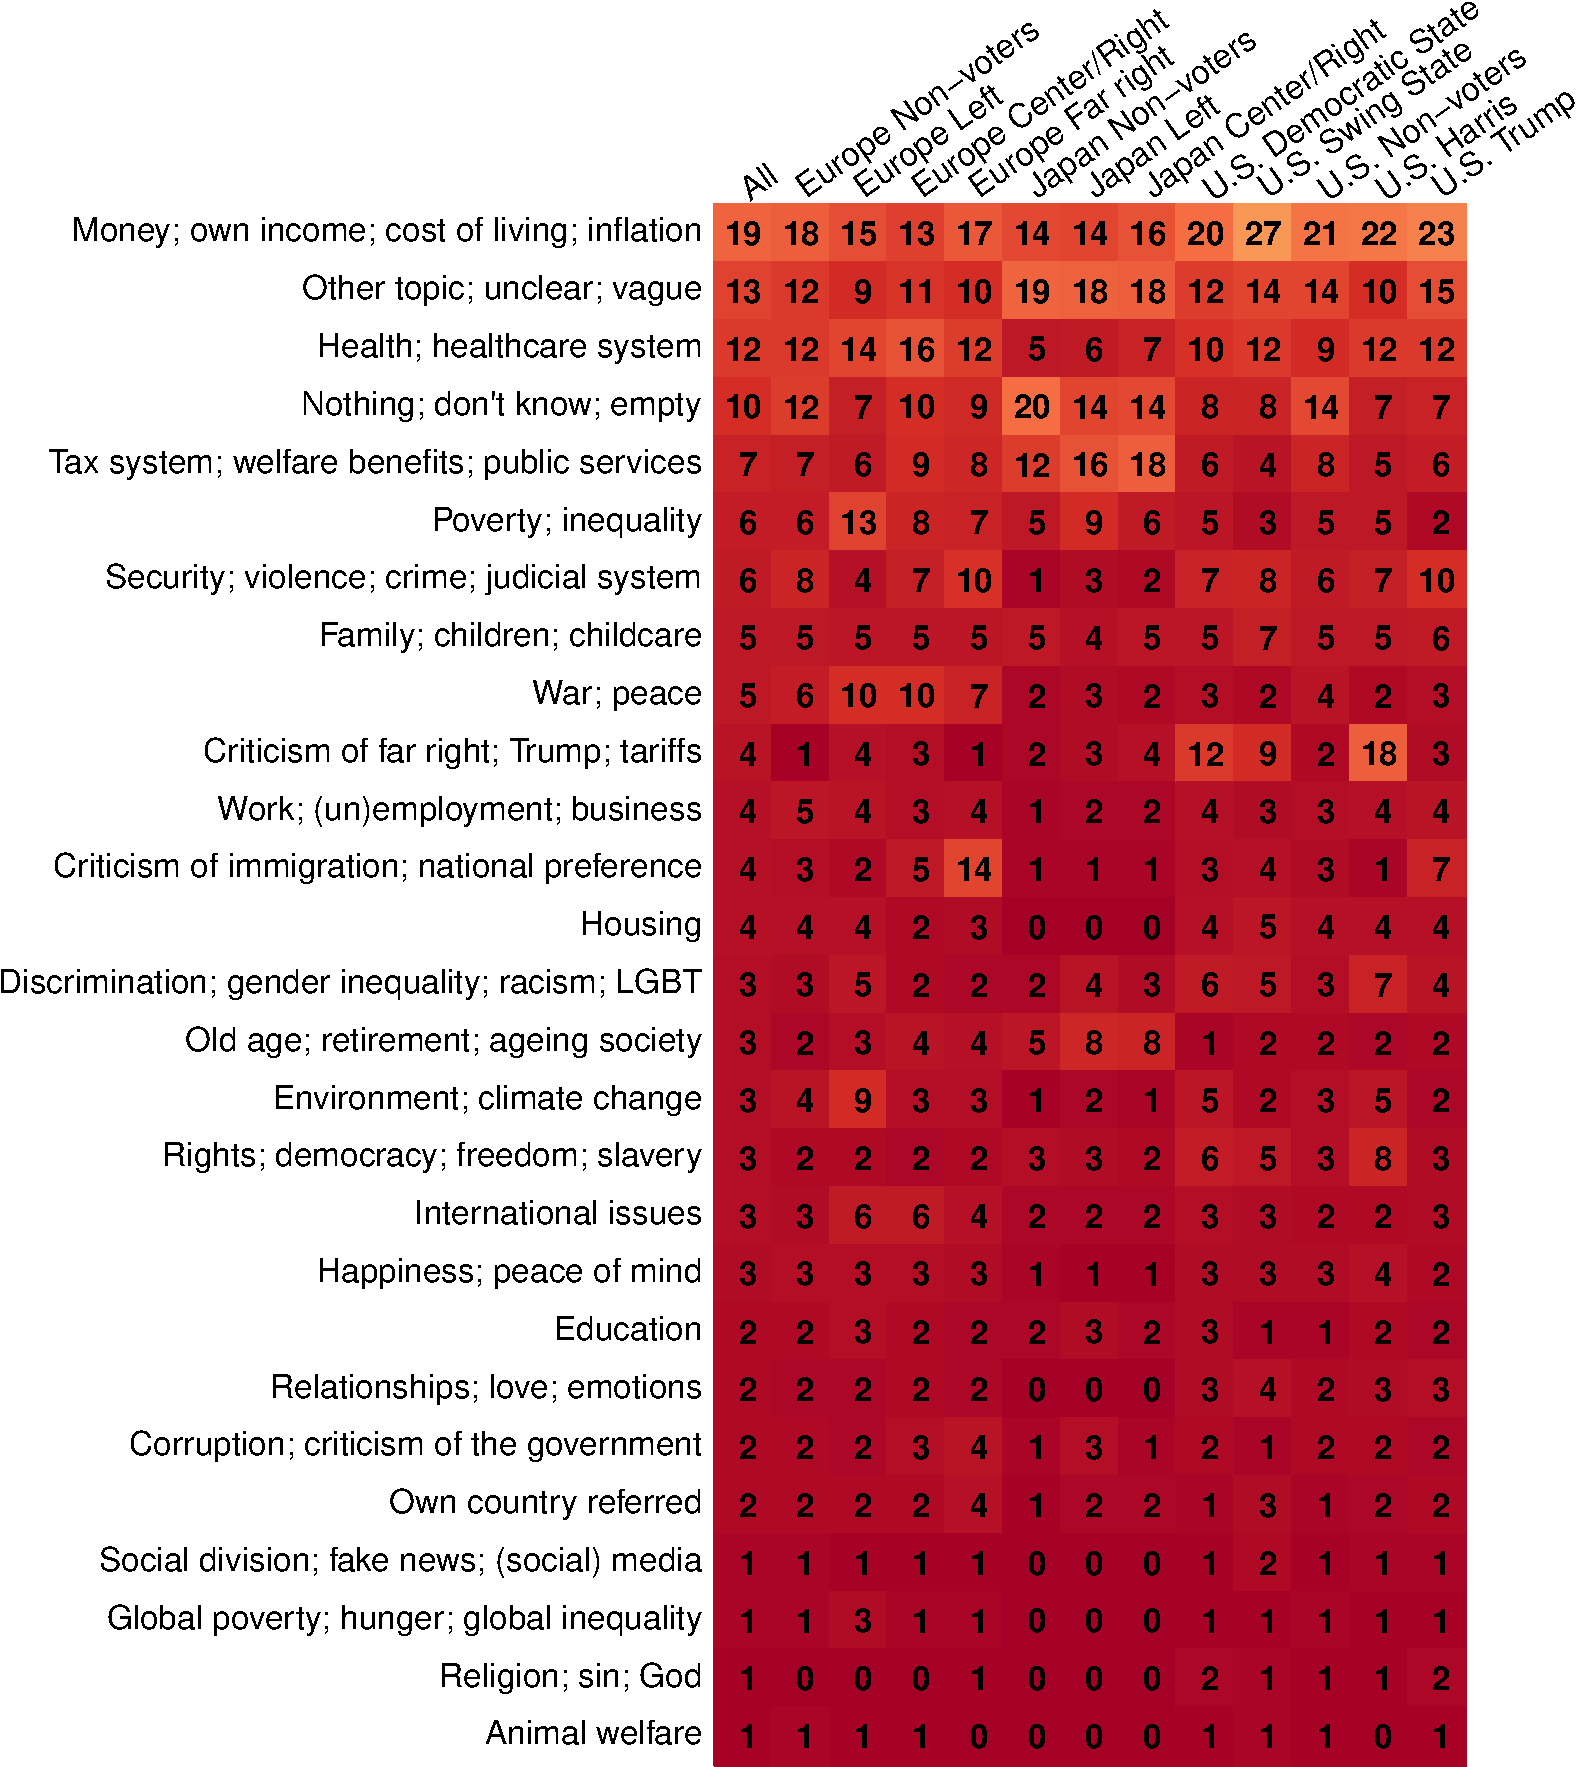
\includegraphics[width=\textwidth]{../figures/country_comparison/field_manual_pol_US_positive.pdf}} 
% \end{figure}
% \hfill (Back~to~Section~\ref{par:representativeness}.)

% \clearpage
% Figures \ref{fig:main_radical_redistr_dem}-\ref{fig:field_manual_dem} show that support for global redistribution is higher among younger, poorer, or more urban people, though the differences are not as large as those between voters of different political orientations. Note that in the following figures, the bottom or top income shares are defined at the national level.

% \begin{figure}[H]
%     \caption[{[}On selected demographics{]} Absolute support for broad global redistribution]{[On selected demographics] Support for global redistribution action/policies. %\hfill (Questions \ref{q:gcs_support}, \ref{q:ics_support}, \ref{q:global_tax_support}-\ref{q:intl_tax_support}, \ref{q:sustainable_future}-\ref{q:top3_tax_support}, \ref{q:convergence_support}-\ref{q:vote_intl_coalition}, \ref{q:reparations_support}, \ref{q:my_tax_global_nation}).
%     }\label{fig:main_radical_redistr_dem} 
%     \makebox[\textwidth][c]{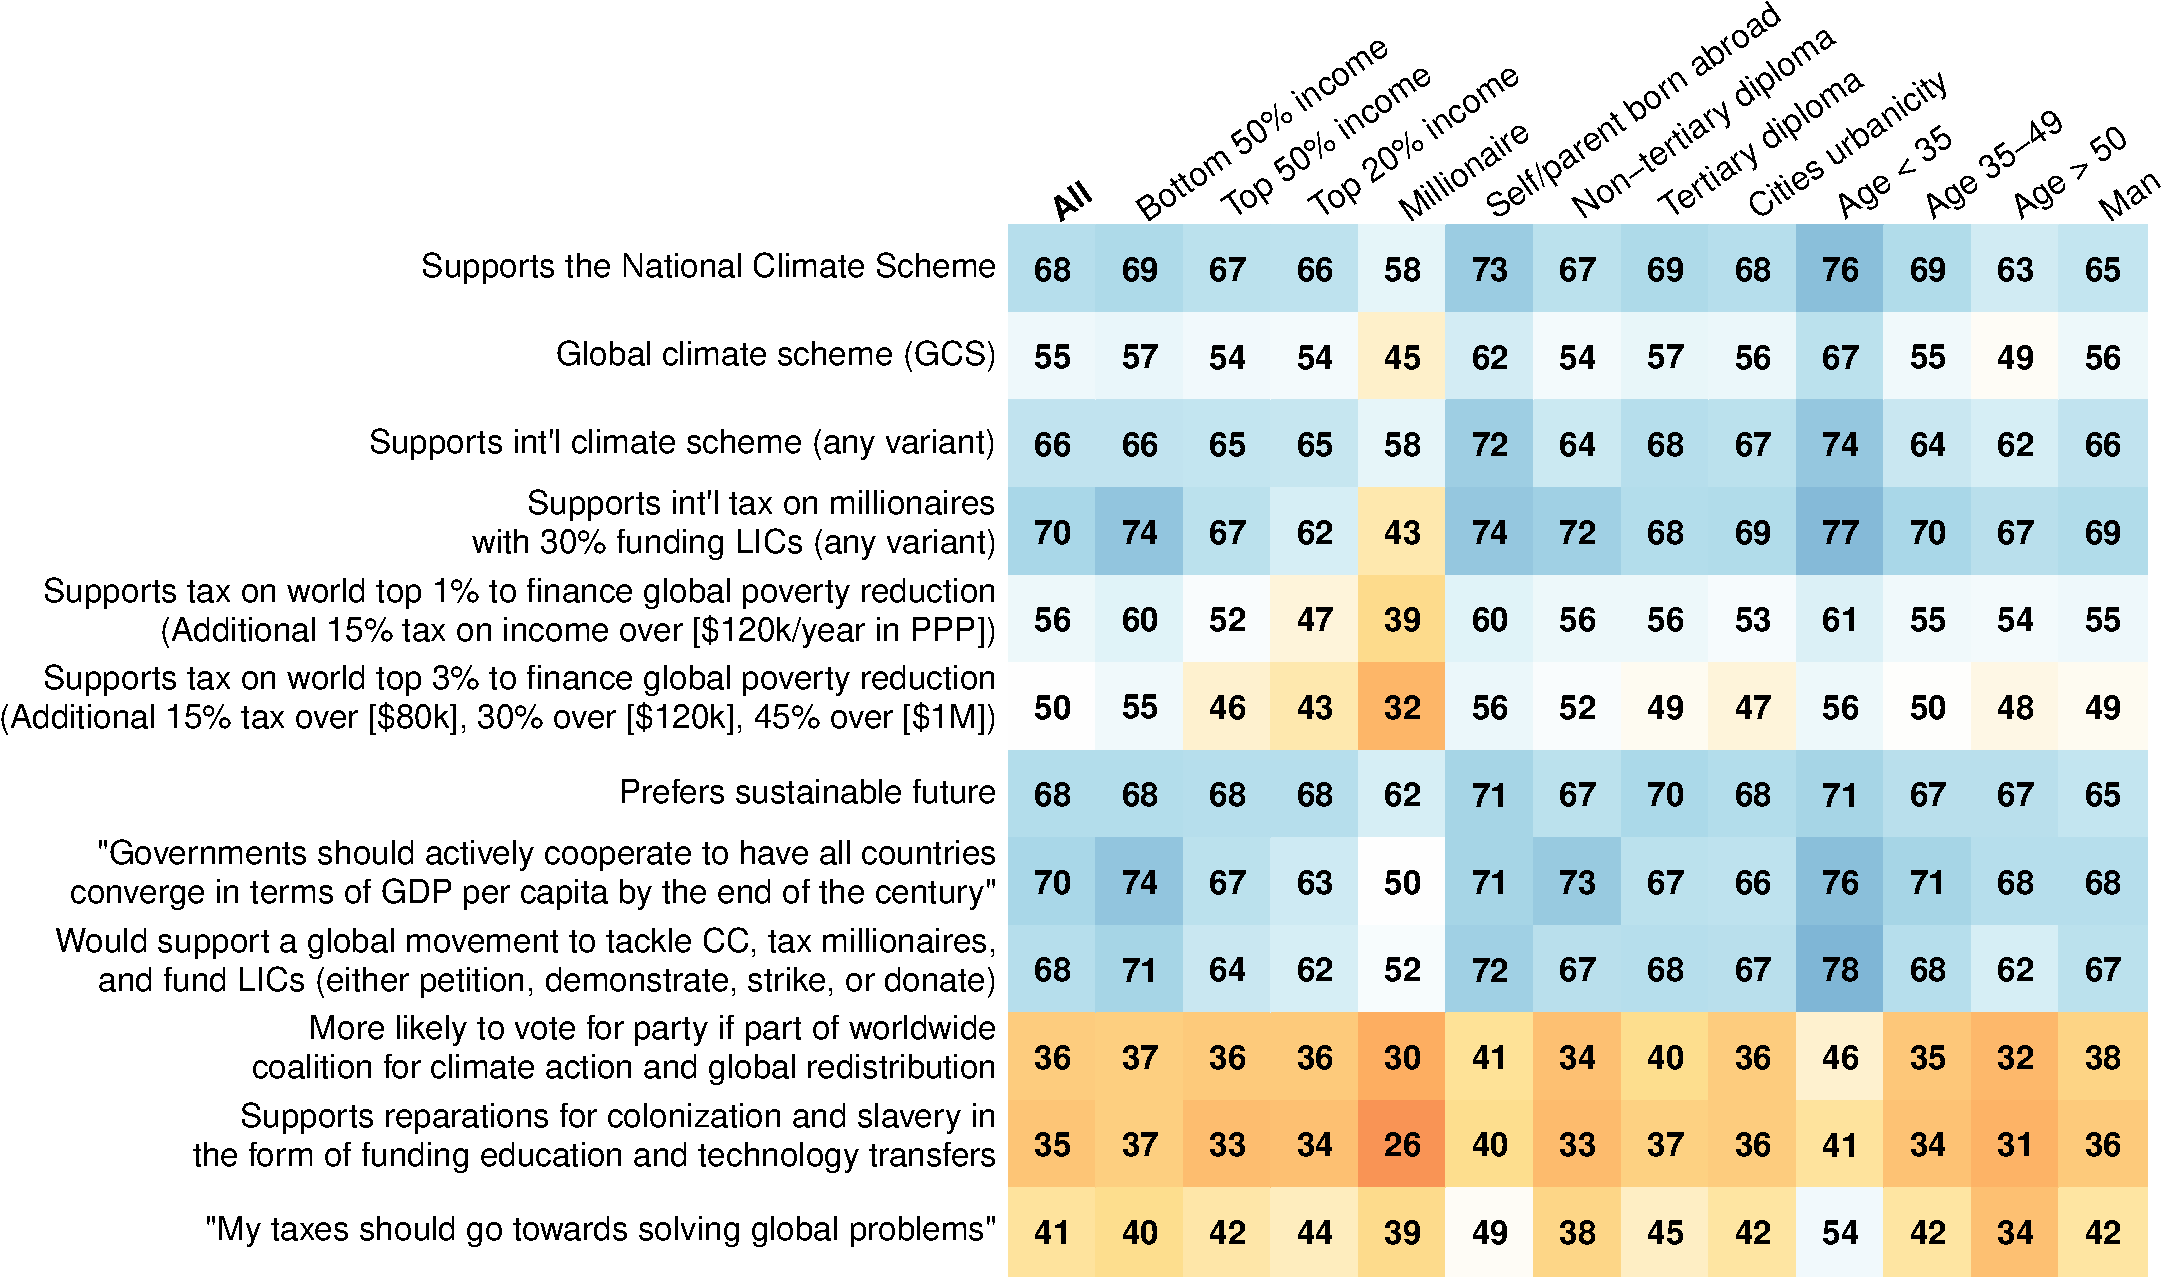
\includegraphics[width=\textwidth]{../figures/country_comparison/main_radical_redistr_dem_positive.pdf}} 
% \end{figure}
% \hfill (Back~to~Section~\ref{par:representativeness}.)

% \begin{figure}[H]
%     \caption[{[}On selected demographics{]} Acceptance of plausible global policies]{[On selected demographics] Acceptance of plausible global redistribution policies (Percentage of \textit{Somewhat} or \textit{Strongly support} among non-\textit{Indifferent} responses). %(Question~\ref{q:solidarity_support}).
%     }\label{fig:solidarity_support_dem_share}
%     \makebox[\textwidth][c]{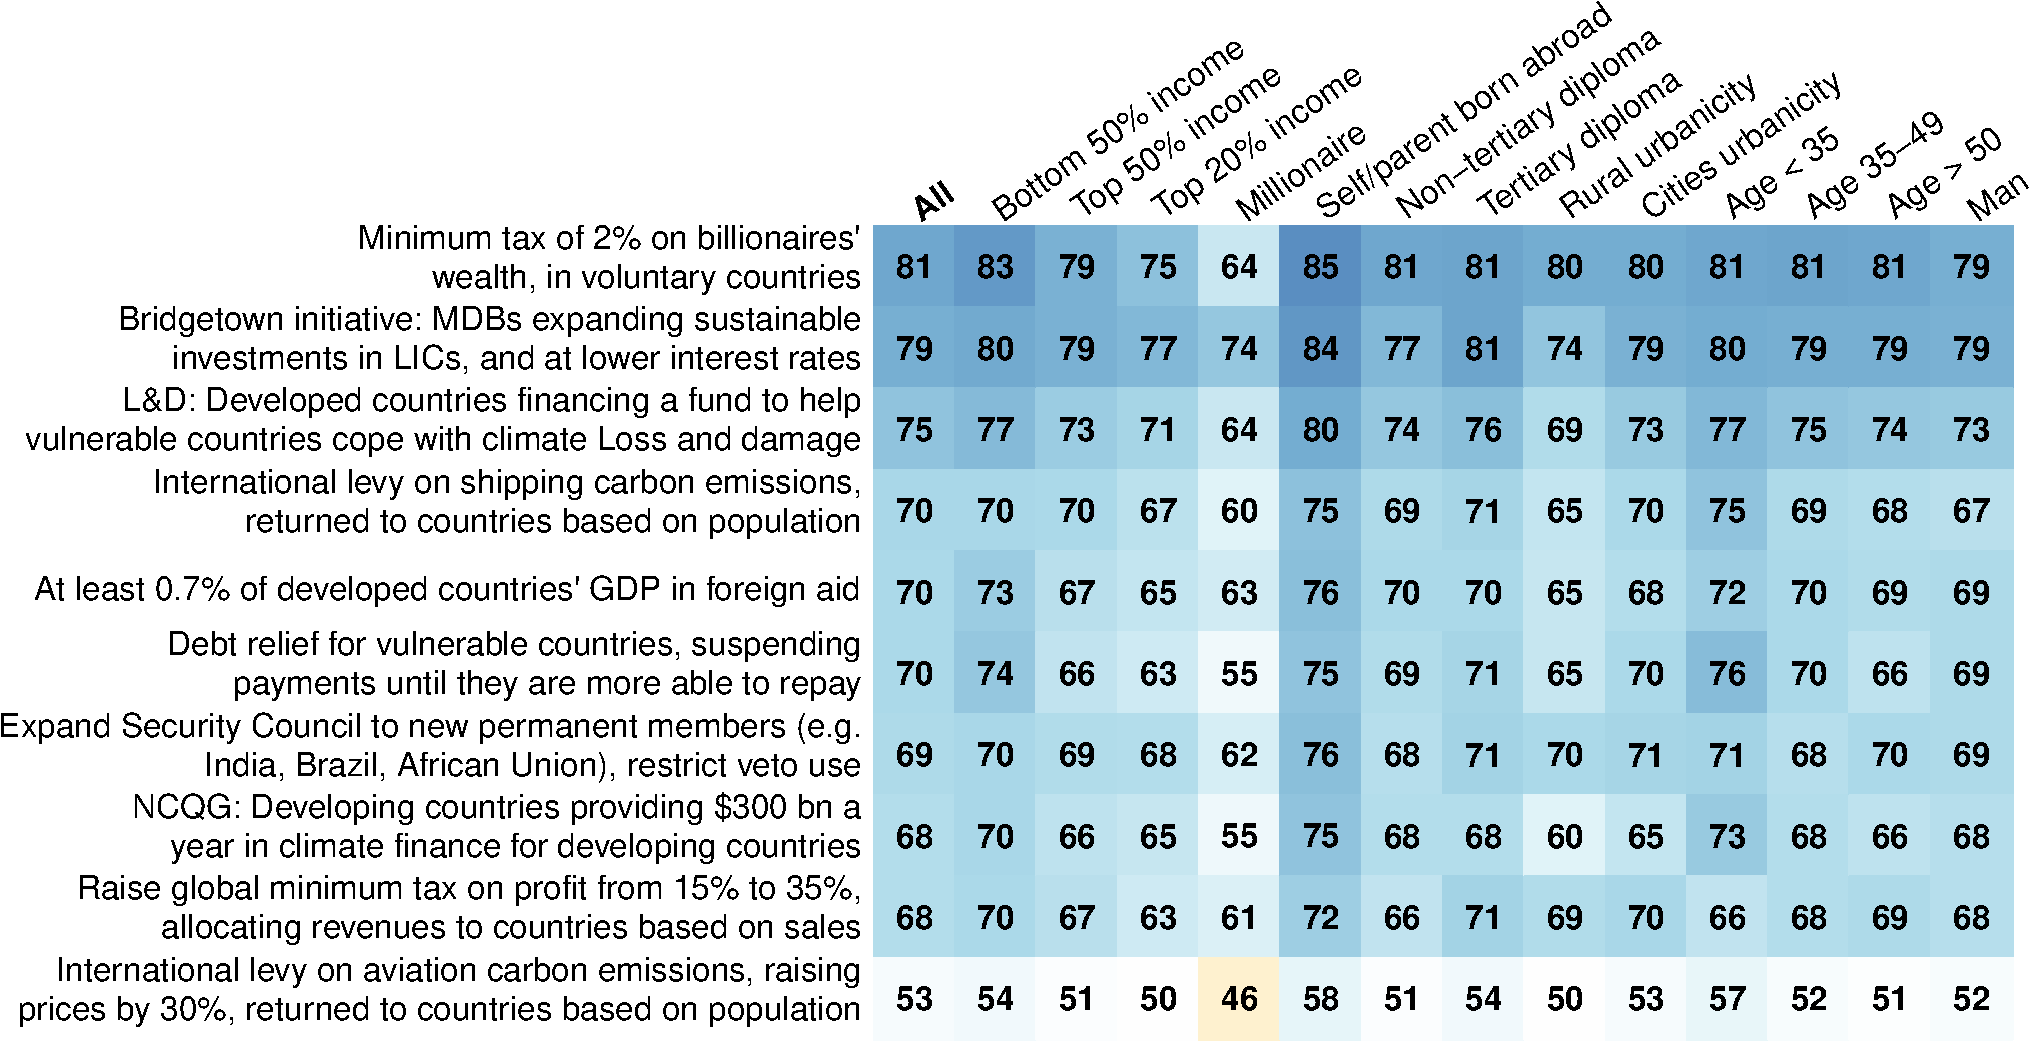
\includegraphics[width=\textwidth]{../figures/country_comparison/solidarity_support_dem_share.pdf}} 
% \end{figure}

\begin{figure}[H]
    \caption[{[}On selected demographics{]} Average synthetic indicators of support]{{[}On selected demographics{]} Average synthetic indicators of support for global redistribution. (Question~\ref{q:solidarity_support}).  \hfill 
    }\label{fig:synthetic_indicators_dem_mean}
    \makebox[\textwidth][c]{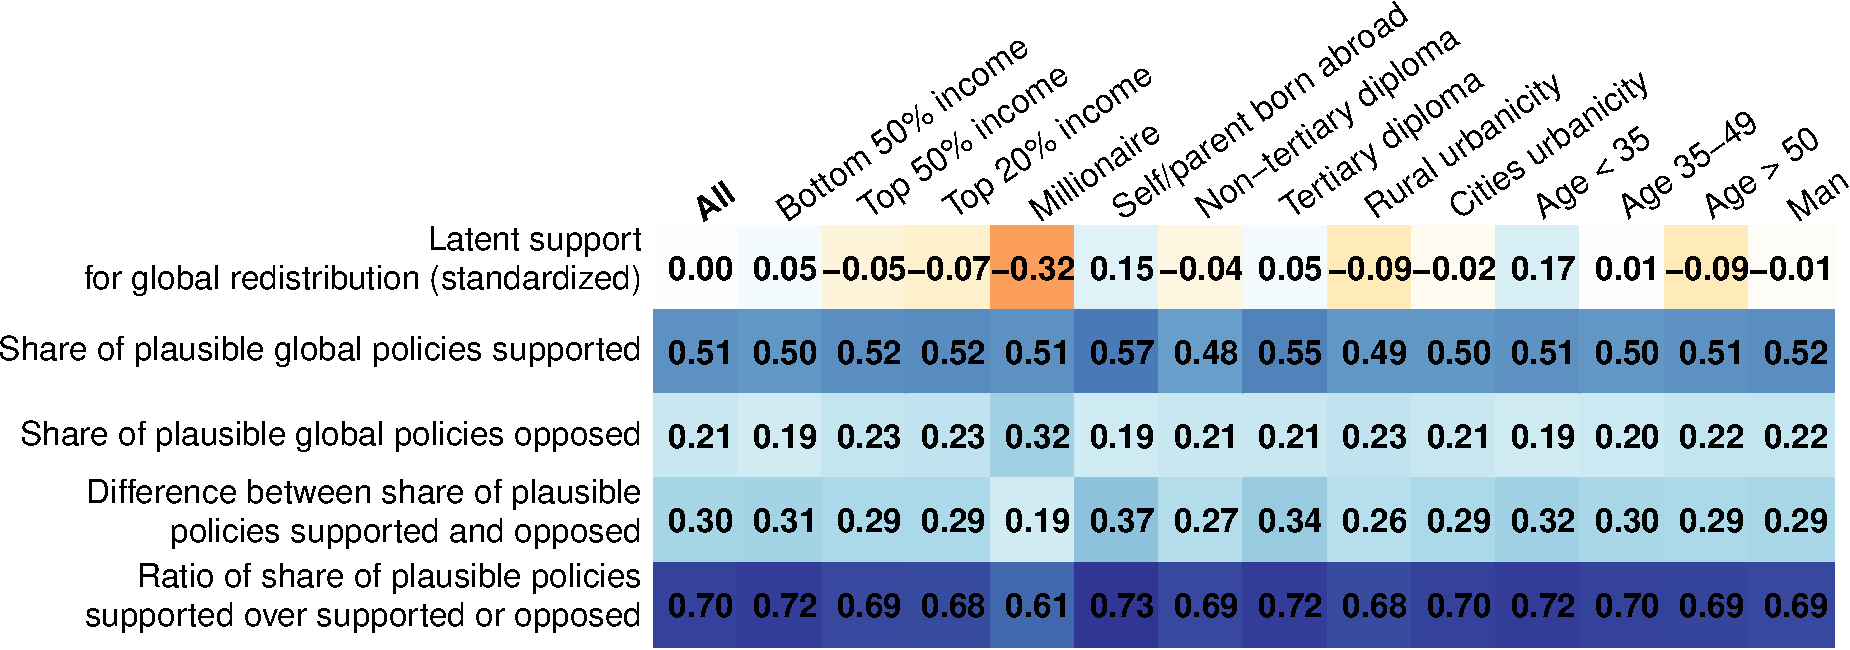
\includegraphics[width=\textwidth]{../figures/country_comparison/synthetic_indicators_dem_mean.pdf}} 
\end{figure}
% \hfill (Back~to~Section~\ref{par:representativeness}.)

% \begin{figure}[H]
%     \caption[{[}On selected demographics{]} Manual classification of open-ended fields]{{[}On selected demographics{]} Manual classification of open-ended fields. (Questions~\ref{q:concerns_field}-\ref{q:injustice_field}).\hfill (Back~to~Section~\ref{subsec:considerations}.)
%     }\label{fig:field_manual_dem}
%     \makebox[\textwidth][c]{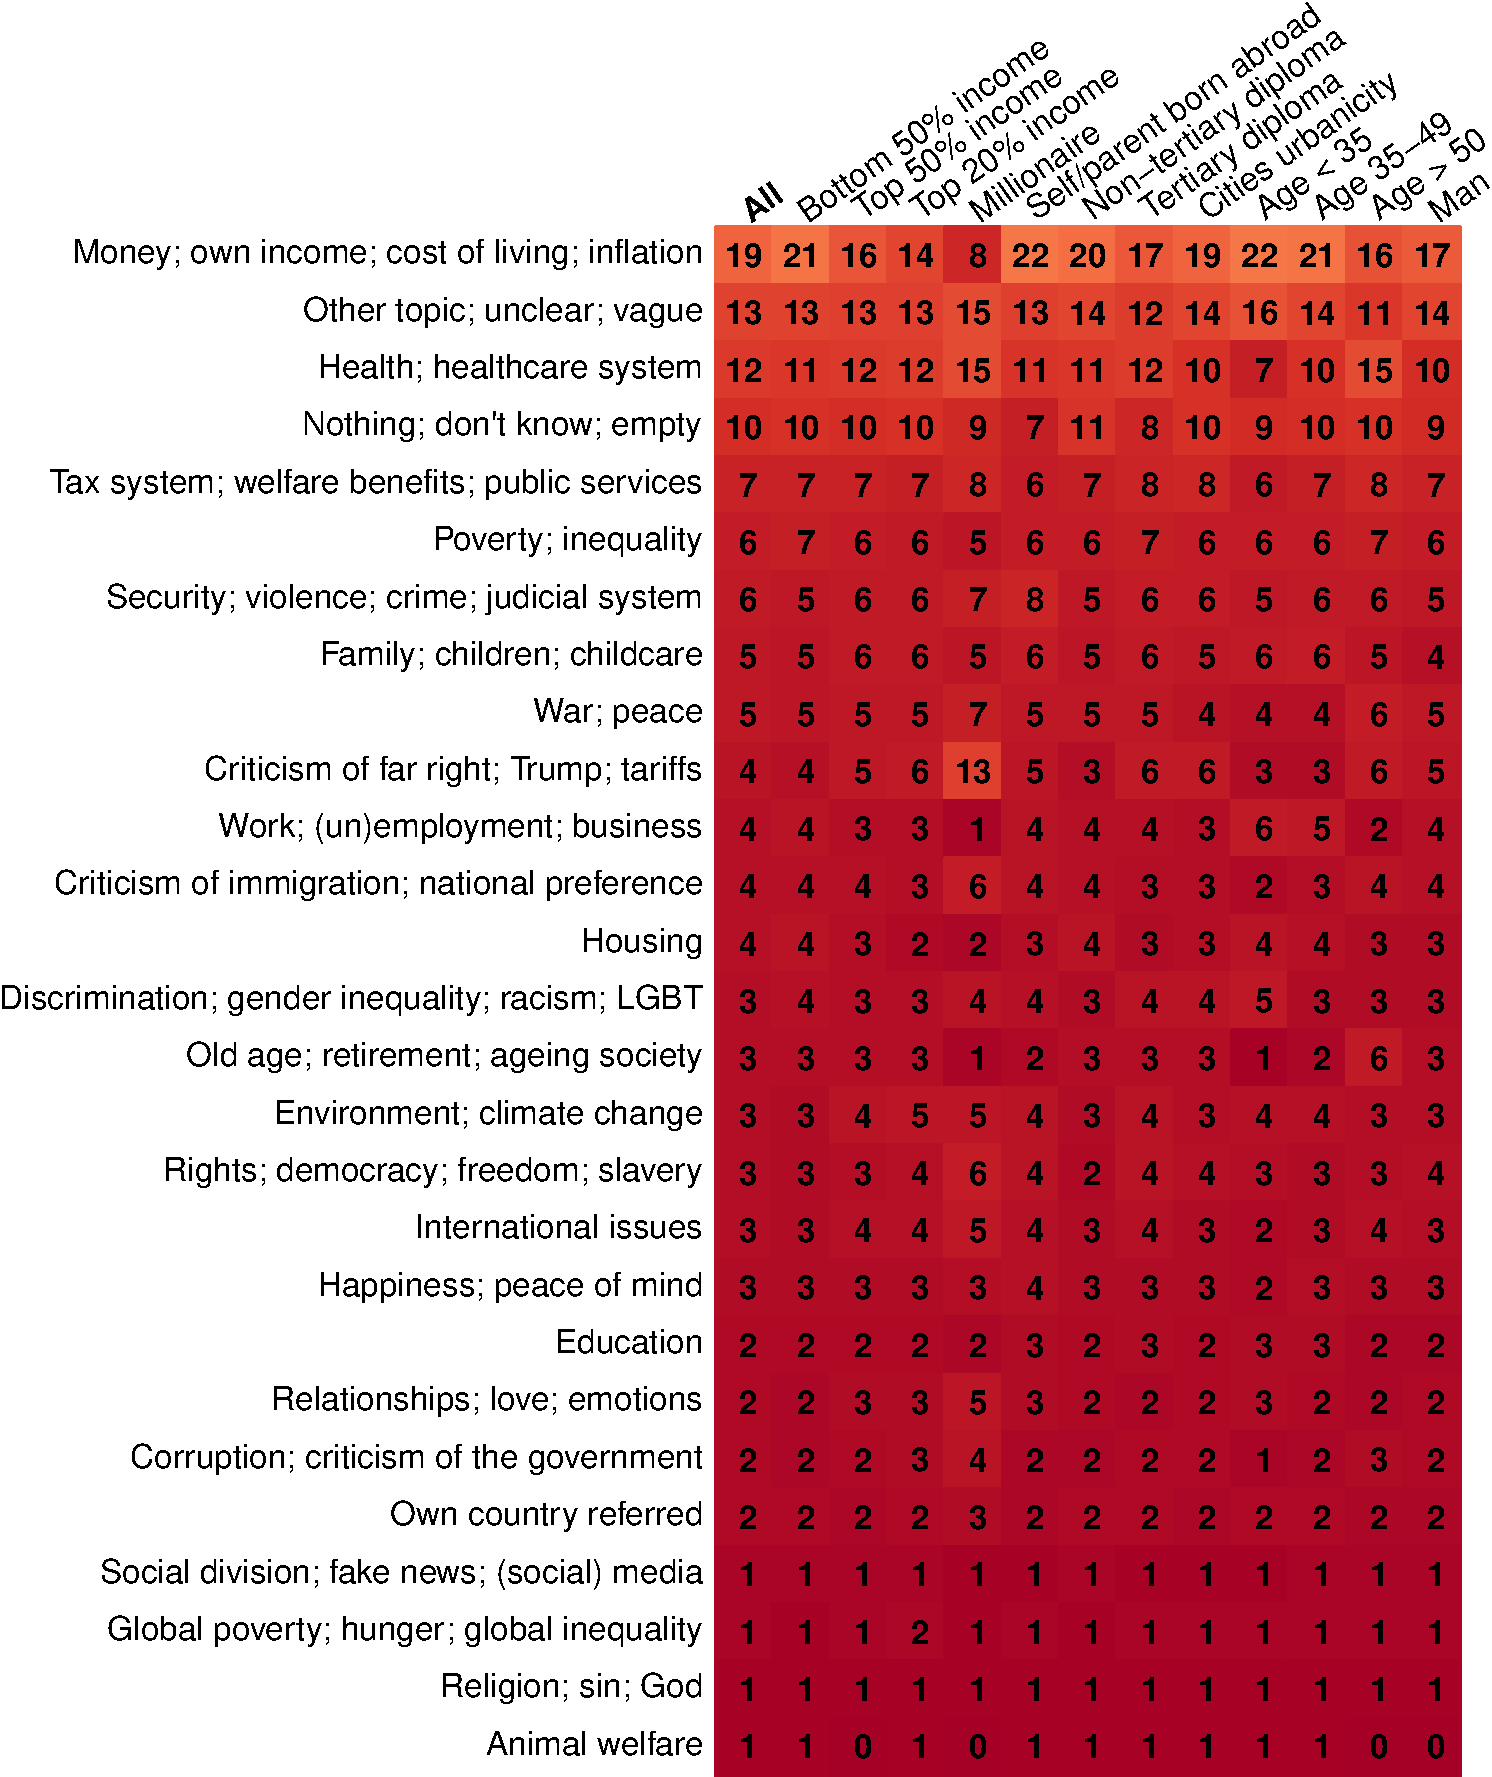
\includegraphics[width=\textwidth]{../figures/country_comparison/field_manual_dem_positive.pdf}} 
% \end{figure}
% \hfill (Back~to~Section~\ref{par:representativeness}.)

% \clearpage
% \section{Main Results Weighted by Vote}\label{app:vote}
% % TODO? Replace the next 2 or 4 figures by main_radical_redistr_weight_vote_share?
% \begin{figure}[H]
%     \caption[{[}Weighted by vote{]} Support for the NCS, GCS, ICS]{[Weighted by vote] Support for the National, Global, and International Climate Schemes (\textit{Yes}/\textit{No} question). \hfill (Questions~\ref{q:ncs_support}-\ref{q:ics_support}).
%     }\label{fig:ics_weight_vote}
%     \makebox[\textwidth][c]{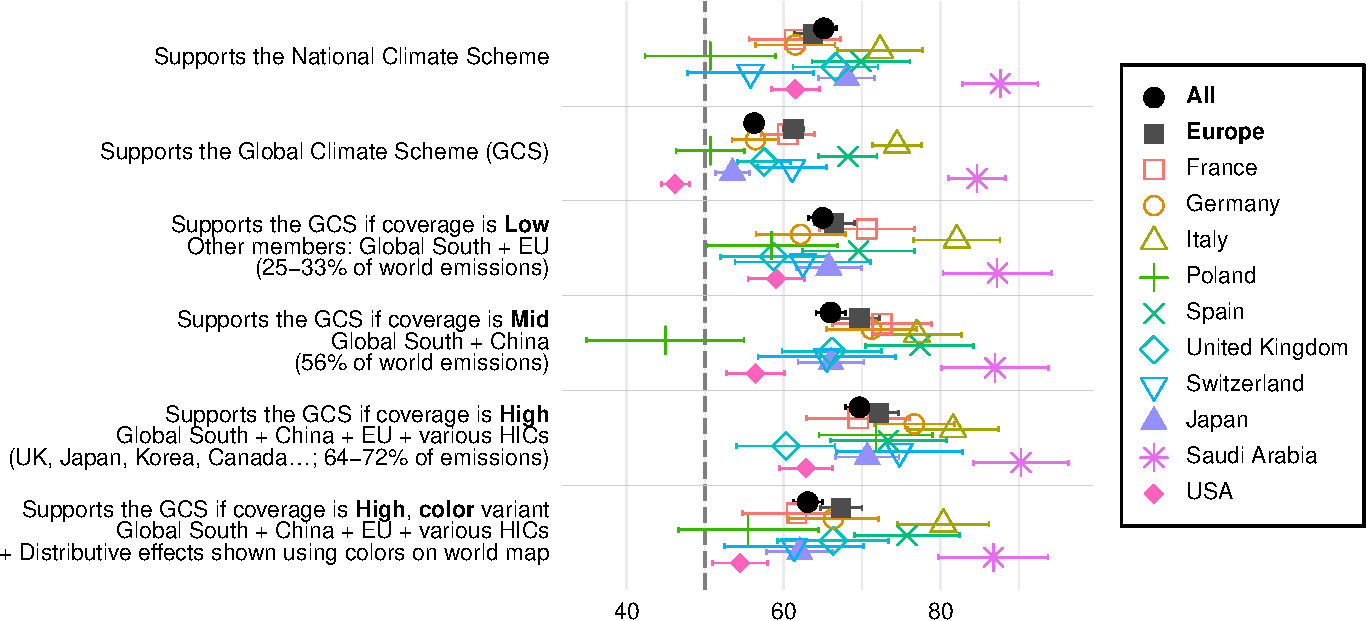
\includegraphics[width=\textwidth]{../figures/country_comparison/variables_ncs_gcs_ics_by_country_weight_vote.pdf}} 
% \end{figure}

% \begin{figure}[H]
%     \caption[{[}Weighted by vote{]} Support for an int'l wealth tax depending on coverage]{[Weighted by vote] Support for an international wealth tax with 30\% of revenue funding LICs, depending on the country coverage (\textit{Yes}/\textit{No} question). \hfill (Questions~\ref{q:global_tax_support}-\ref{q:intl_tax_support}).
%     }\label{fig:wealth_tax_weight_vote}
%     \makebox[\textwidth][c]{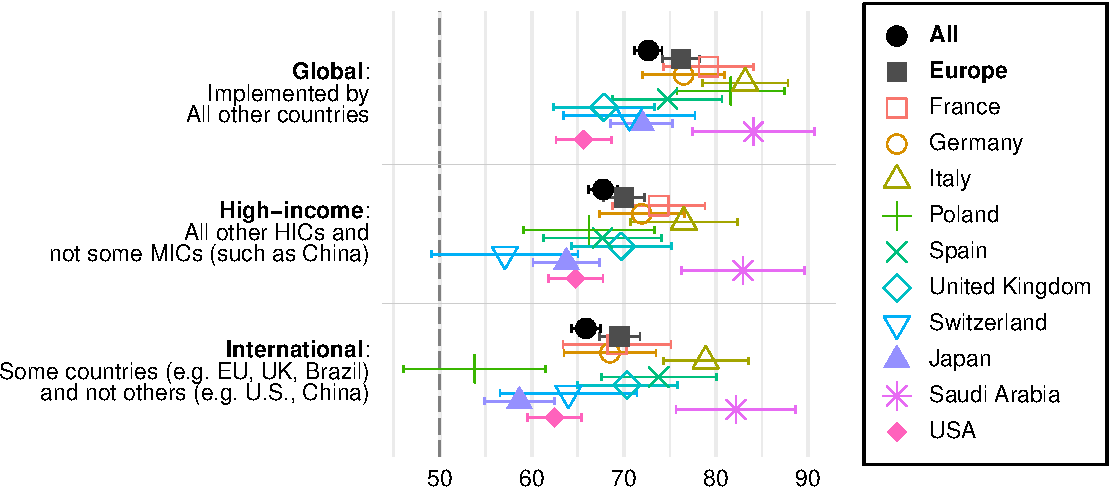
\includegraphics[width=.9\textwidth]{../figures/country_comparison/variables_wealth_tax_support_by_country_weight_vote.pdf}} 
% \end{figure}
% \hfill (Back~to~Section~\ref{par:representativeness}.)

% \begin{figure}[H]
% \caption[{[}Weighted by vote{]} Conjoint analysis]{[Weighted by vote] Effect on the likelihood that a political program is preferred of containing the following policy (compared to no foreign policy in the program). \hfill (Question~\ref{q:conjoint})} \label{fig:conjoint_weight_vote}
% \begin{subfigure}{.49\textwidth}
%   \caption[]{Cut development aid}
%   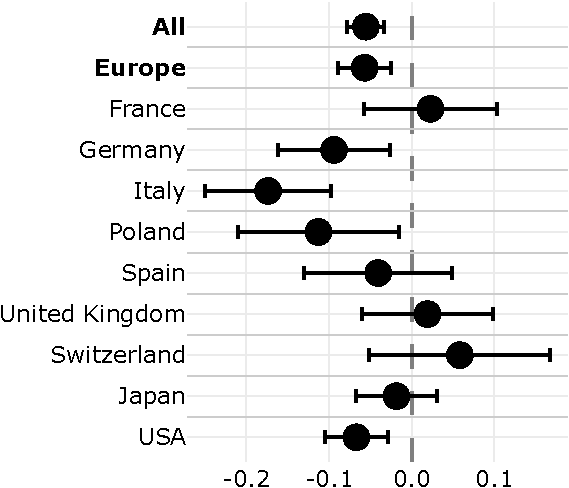
\includegraphics[height=.33\textheight]{../figures/country_comparison/program_preferred_by_cut_aid_in_program_weight_vote.pdf}
% \end{subfigure} 
% \begin{subfigure}{.49\textwidth}
%   \caption[]{International tax on millionaires with 30\% financing health and education in low-income countries}%\begin{flushright}
%   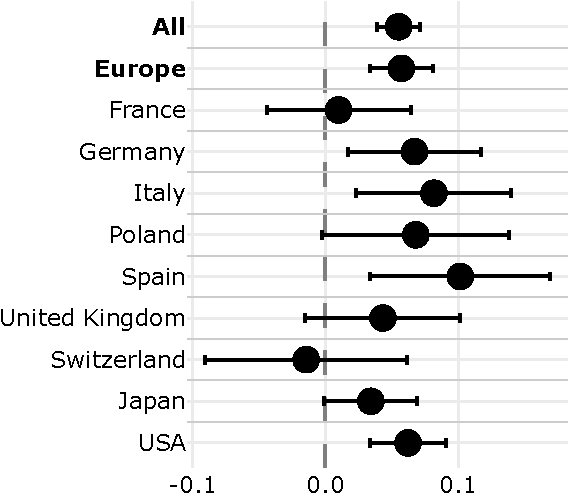
\includegraphics[height=.33\textheight]{../figures/country_comparison/program_preferred_by_millionaire_tax_in_program_weight_vote.pdf}%\end{flushright}
% \end{subfigure}
% \end{figure}

% \begin{figure}[H]
% \caption[{[}Weighted by vote{]} Testing warm glow]{[Weighted by vote] Testing warm glow (negative effects would indicate the presence of warm glow).}\label{fig:warm_glow_weight_vote}
% \begin{subfigure}{.45\textwidth}
%   \caption[]{Effect of a \textit{Donation lottery} treatment on support for the Global Climate Scheme. (Questions~\ref{q:donation}-\ref{q:gcs_support})\label{fig:warm_glow_substitute_weight_vote}}
%   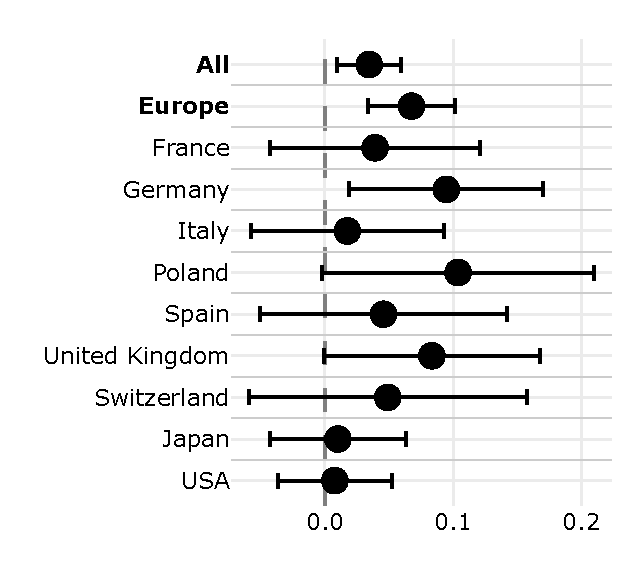
\includegraphics[height=.33\textheight]{../figures/country_comparison/gcs_support_by_variant_warm_glow_weight_vote.pdf}
% \end{subfigure} \quad
% \begin{subfigure}{.49\textwidth}
%   \caption[]{Effect of information about ongoing global redistribution initiatives on the share of plausible global policies supported. (Questions~\ref{q:info_solidarity}-\ref{q:solidarity_support})\label{fig:warm_glow_realism_weight_vote}}
%   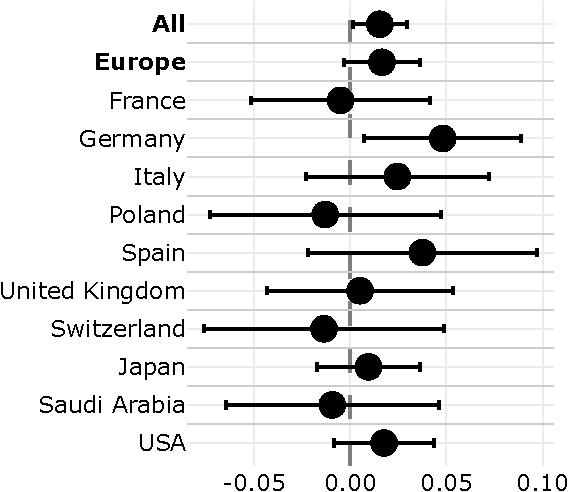
\includegraphics[height=.33\textheight]{../figures/country_comparison/share_solidarity_supported_by_info_solidarity_weight_vote.pdf}
% \end{subfigure}
% \end{figure}

% \begin{figure}[H]
%     \caption[{[}Weighted by vote{]} Acceptance of plausible global policies]{[Weighted by vote] Acceptance of plausible global redistribution policies (Percentage of \textit{Somewhat} or \textit{Strongly support} among non-\textit{Indifferent} responses). (Question~\ref{q:solidarity_support}).
%     }\label{fig:solidarity_support_share_weight_vote}
%     \makebox[\textwidth][c]{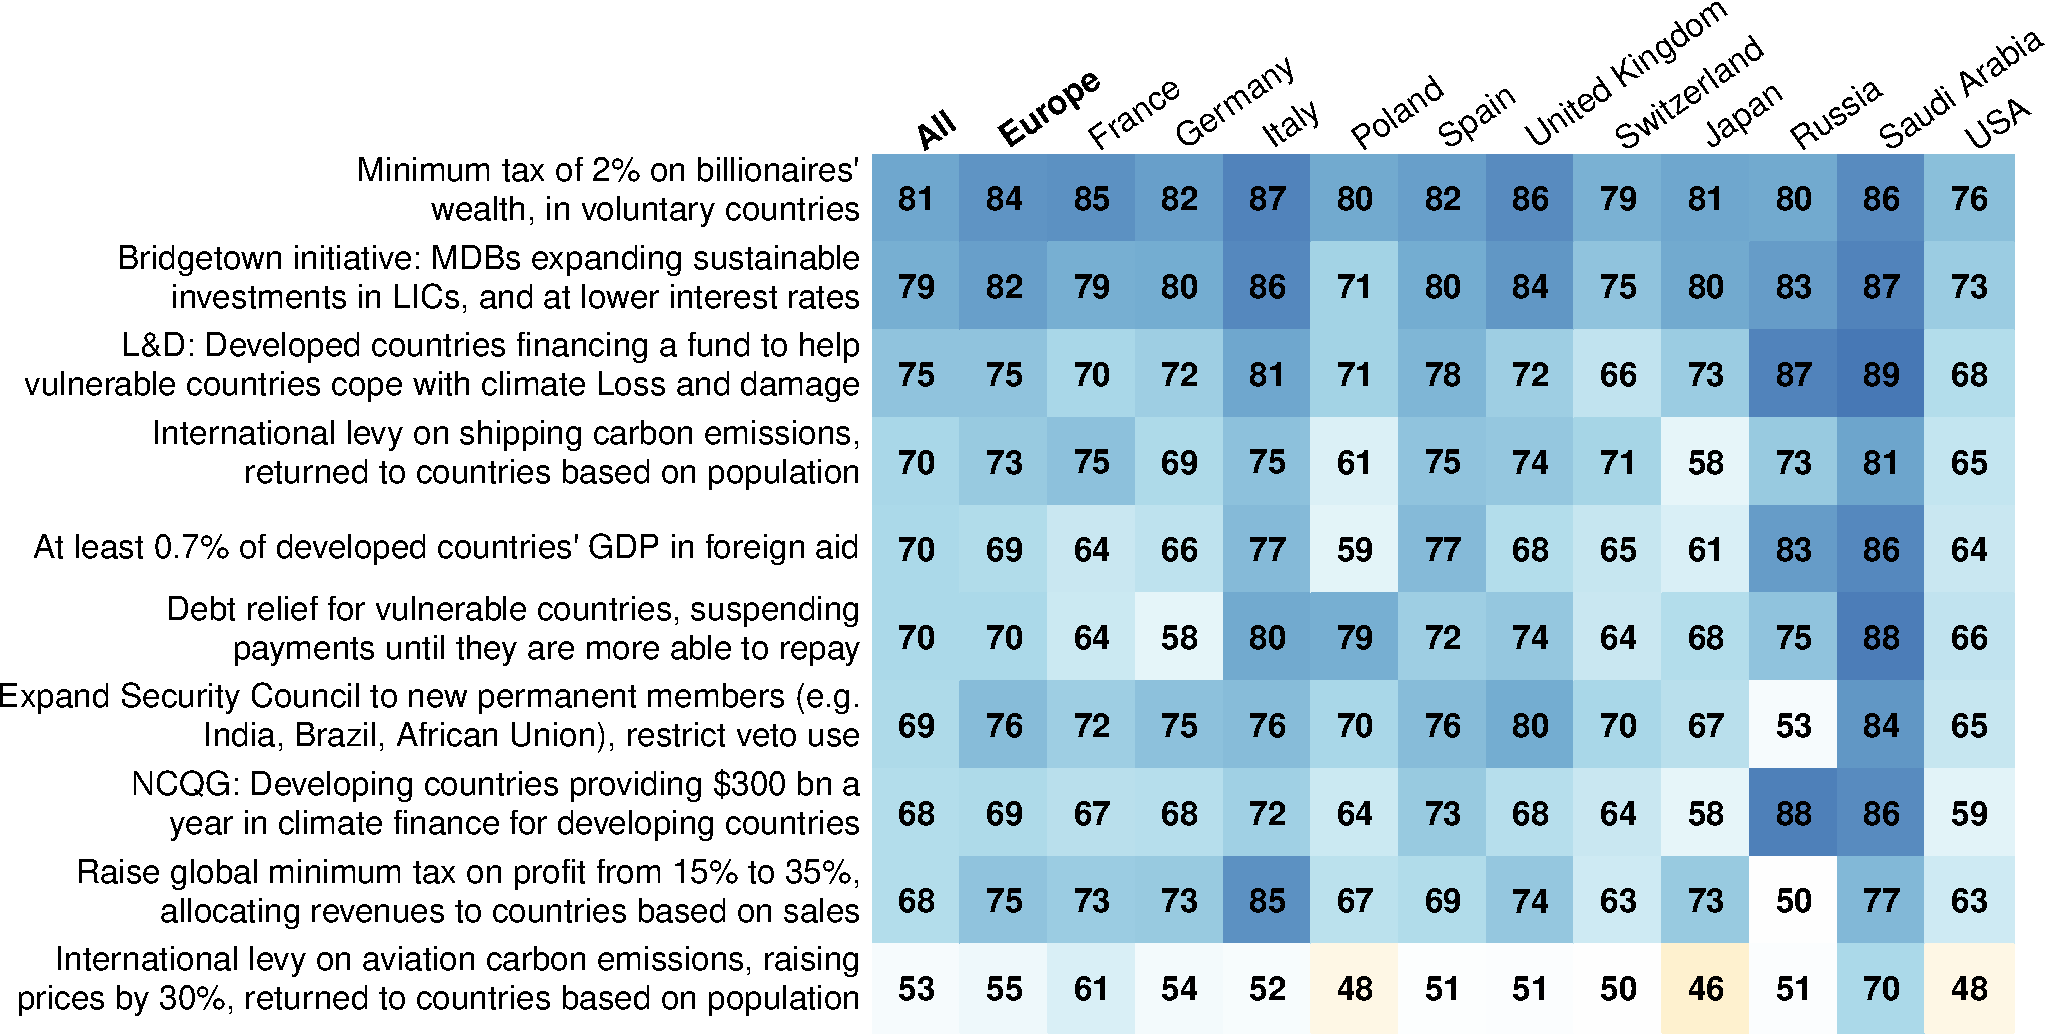
\includegraphics[width=\textwidth]{../figures/country_comparison/solidarity_support_weight_vote_share.pdf}} 
% \end{figure}
% % # 9. radical_redistr: 
% \begin{figure}[H]
%     \caption[{[}Weighted by vote{]} Support for broad or radical global redistribution]{[Weighted by vote] Support for broad action or radical proposals of global redistribution. \hfill (Questions~\ref{q:sustainable_future}-\ref{q:top3_tax_support}, \ref{q:convergence_support}-\ref{q:vote_intl_coalition}, \ref{q:reparations_support}, \ref{q:my_tax_global_nation}).
%     }\label{fig:radical_redistr_share_weight_vote} 
%     \makebox[\textwidth][c]{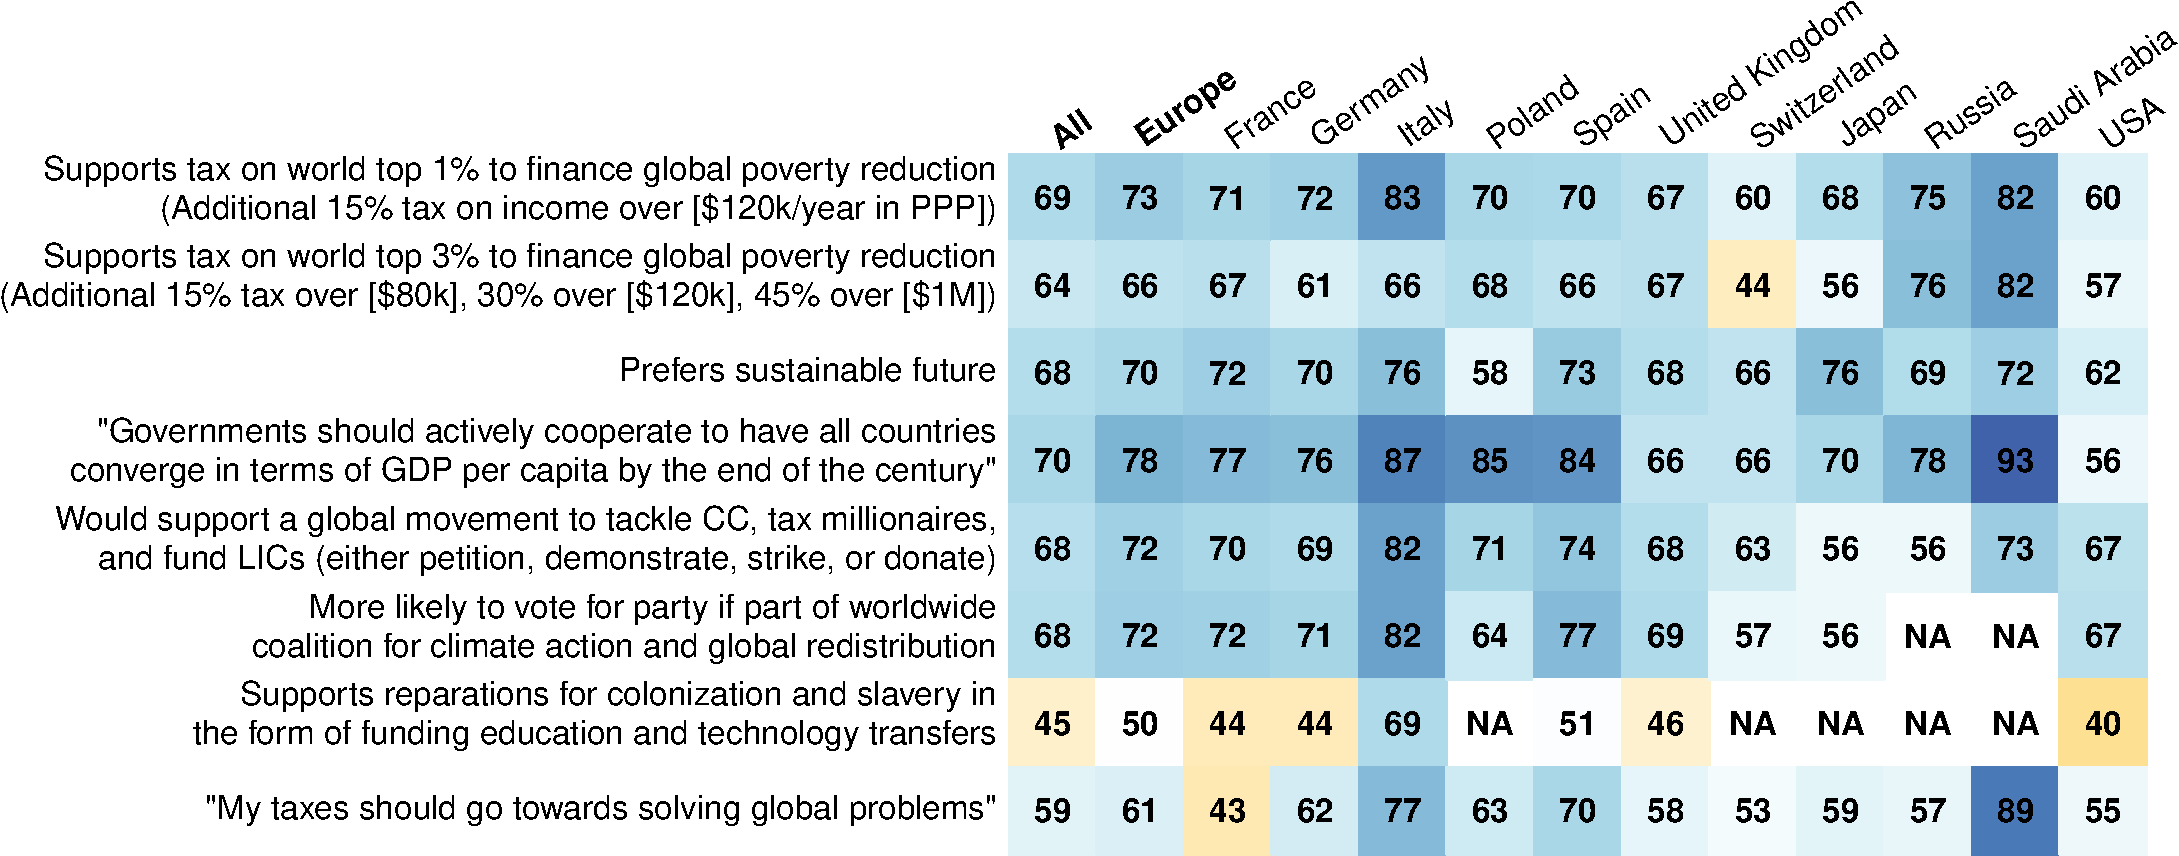
\includegraphics[width=\textwidth]{../figures/country_comparison/radical_redistr_weight_vote_share.pdf}} 
% \end{figure}
% \hfill (Back~to~Section~\ref{par:representativeness}.)

% \clearpage
% \section{Main Results on the Extended Sample}\label{app:extended}

% % As a robustness check, we reproduce our main results on the extended sample that includes the 14\% respondents who failed the attention check or rushed through the survey ($n = 9,318$). These results are non-weighted. They closely match the results in our main specification. For example, the support for the GCS is 54\% in the U.S. and 75\% in Europe, while the same coefficients are significant for the list experiment. % and the conjoint analyses. 

% % \begin{figure}[h!] 
% %     \caption[(Extended sample) Main attitudes]{[Extended sample] Main attitudes. \\ (Relative support ---unless *--- in percent in Questions~\ref{q:gcs_support}, \ref{q:global_tax}, \ref{q:other_policies}, \ref{q:foreign_aid_raise_support}, \ref{q:negotiation}) \hfill (Back~to~Section~\ref{subsec:universalistic})}\label{fig:main_by_vote_alla}
% %     \makebox[\textwidth][c]{\includegraphics[width=\textwidth]{../figures/country_comparison/main_alla_share.pdf}} 
% % \end{figure}


% \begin{figure}[H]
%     \caption[{[}Extended sample{]} Support for the NCS, GCS, ICS]{[Extended sample] Support for the National, Global, and International Climate Schemes (\textit{Yes}/\textit{No} question). \hfill (Questions~\ref{q:ncs_support}-\ref{q:ics_support}).
%     }\label{fig:ics_extended}
%     \makebox[\textwidth][c]{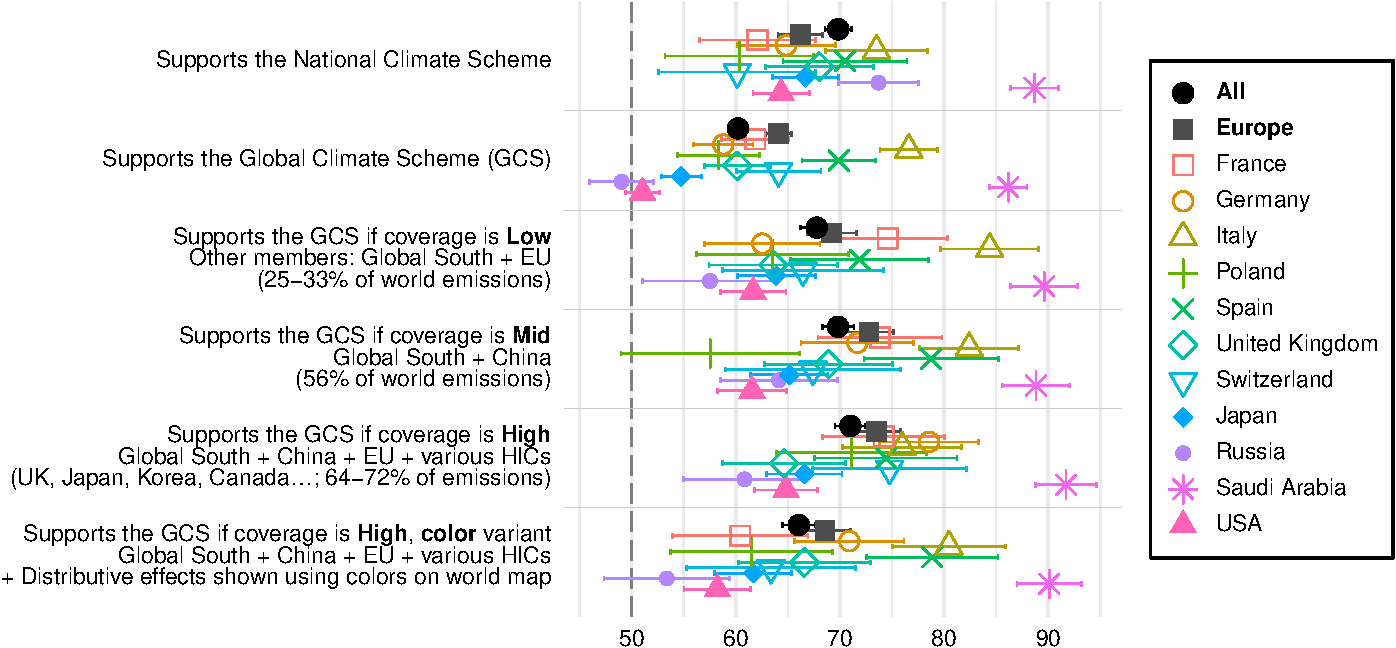
\includegraphics[width=\textwidth]{../figures/country_comparison/variables_ncs_gcs_ics_by_country_extended.pdf}} 
% \end{figure}

% \begin{figure}[H]
%     \caption[{[}Extended sample{]} Support for an int'l wealth tax depending on coverage]{[Extended sample] Support for an international wealth tax with 30\% of revenue funding LICs, depending on the country coverage (\textit{Yes}/\textit{No} question). \hfill (Questions~\ref{q:global_tax_support}-\ref{q:intl_tax_support}).
%     }\label{fig:wealth_tax_extended}
%     \makebox[\textwidth][c]{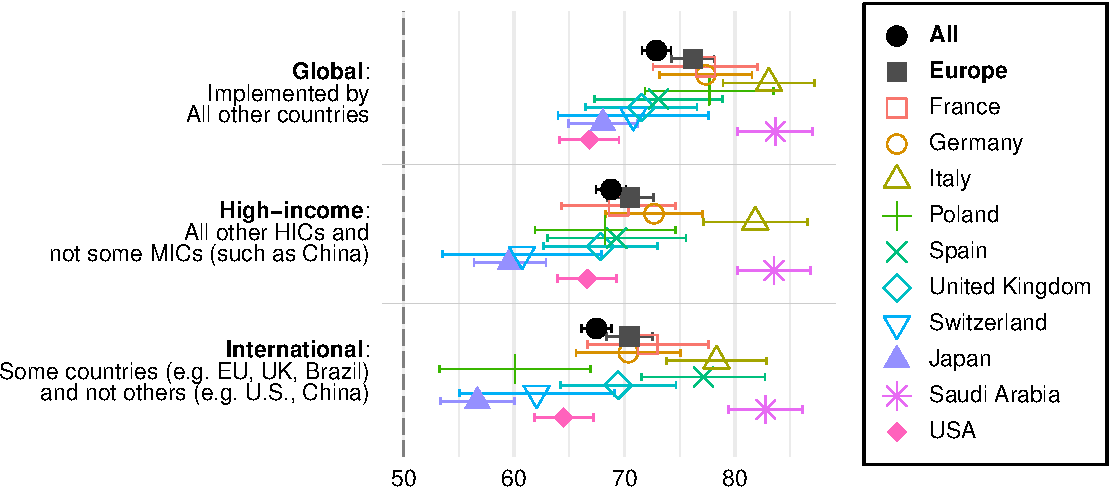
\includegraphics[width=.9\textwidth]{../figures/country_comparison/variables_wealth_tax_support_by_country_extended.pdf}} 
% \end{figure}
% \hfill (Back~to~Section~\ref{par:data_quality}.)

% \begin{figure}[H]
% \caption[{[}Extended sample{]} Conjoint analysis]{[Extended sample] Effect on the likelihood that a political program is preferred of containing the following policy (compared to no foreign policy in the program). \hfill (Question~\ref{q:conjoint})} \label{fig:conjoint_extended}
% \begin{subfigure}{.49\textwidth}
%   \caption[]{Cut development aid}
%   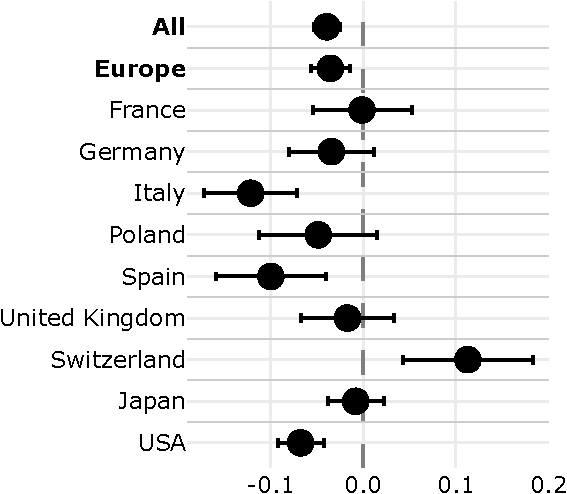
\includegraphics[height=.3\textheight]{../figures/country_comparison/program_preferred_by_cut_aid_in_program_extended.pdf}
% \end{subfigure} 
% \begin{subfigure}{.49\textwidth}
%   \caption[]{International tax on millionaires with 30\% financing health and education in low-income countries}%\begin{flushright}
%   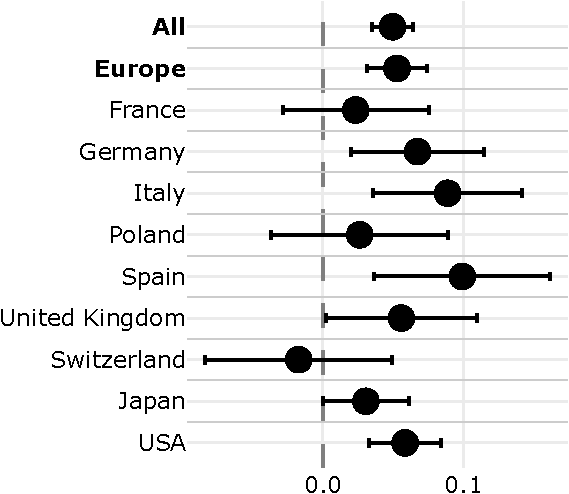
\includegraphics[height=.3\textheight]{../figures/country_comparison/program_preferred_by_millionaire_tax_in_program_extended.pdf}%\end{flushright}
% \end{subfigure}
% \end{figure}

% \begin{figure}[H]
% \caption[{[}Extended sample{]} Testing warm glow]{[Extended sample] Testing warm glow (negative effects would indicate the presence of warm glow).}\label{fig:warm_glow_extended}
% \begin{subfigure}{.45\textwidth}
%   \caption[]{Effect of a \textit{Donation lottery} treatment on support for the Global Climate Scheme. (Questions~\ref{q:donation}-\ref{q:gcs_support})\label{fig:warm_glow_substitute_extended}}
%   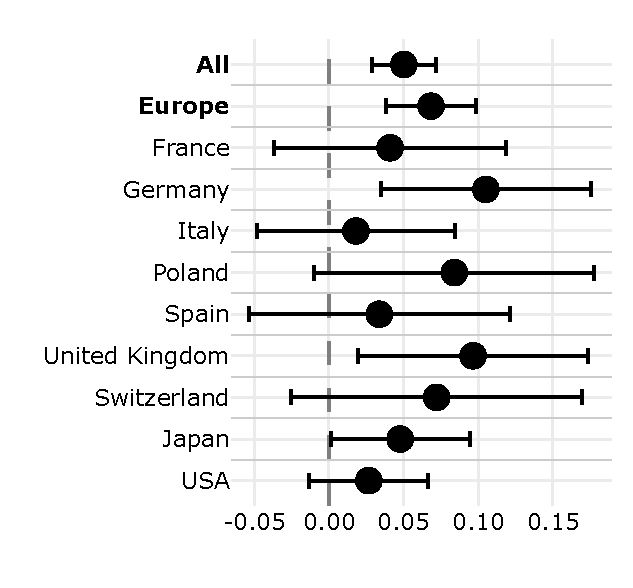
\includegraphics[height=.3\textheight]{../figures/country_comparison/gcs_support_by_variant_warm_glow_extended.pdf}
% \end{subfigure} \quad
% \begin{subfigure}{.49\textwidth}
%   \caption[]{Effect of information about ongoing global redistribution initiatives on the share of plausible global policies supported. (Questions~\ref{q:info_solidarity}-\ref{q:solidarity_support})\label{fig:warm_glow_realism_extended}}
%   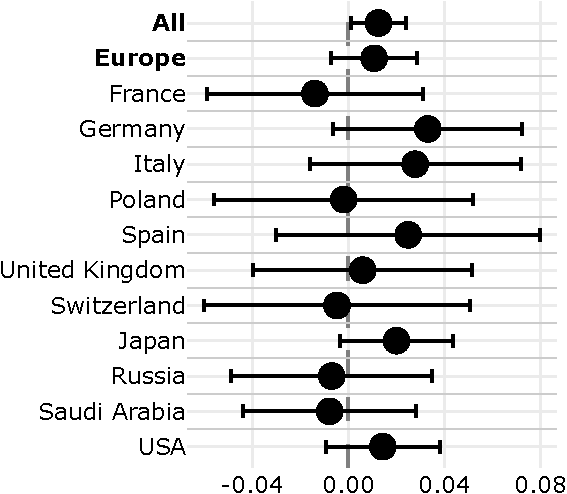
\includegraphics[height=.3\textheight]{../figures/country_comparison/share_solidarity_supported_by_info_solidarity_extended.pdf}
% \end{subfigure}
% \end{figure}

% \begin{figure}[H]
%     \caption[{[}Extended sample{]} Acceptance of plausible global policies]{[Extended sample] Acceptance of plausible global redistribution policies (Percentage of \textit{Somewhat} or \textit{Strongly support} among non-\textit{Indifferent} responses). (Question~\ref{q:solidarity_support}).
%     }\label{fig:solidarity_support_share_extended}
%     \makebox[\textwidth][c]{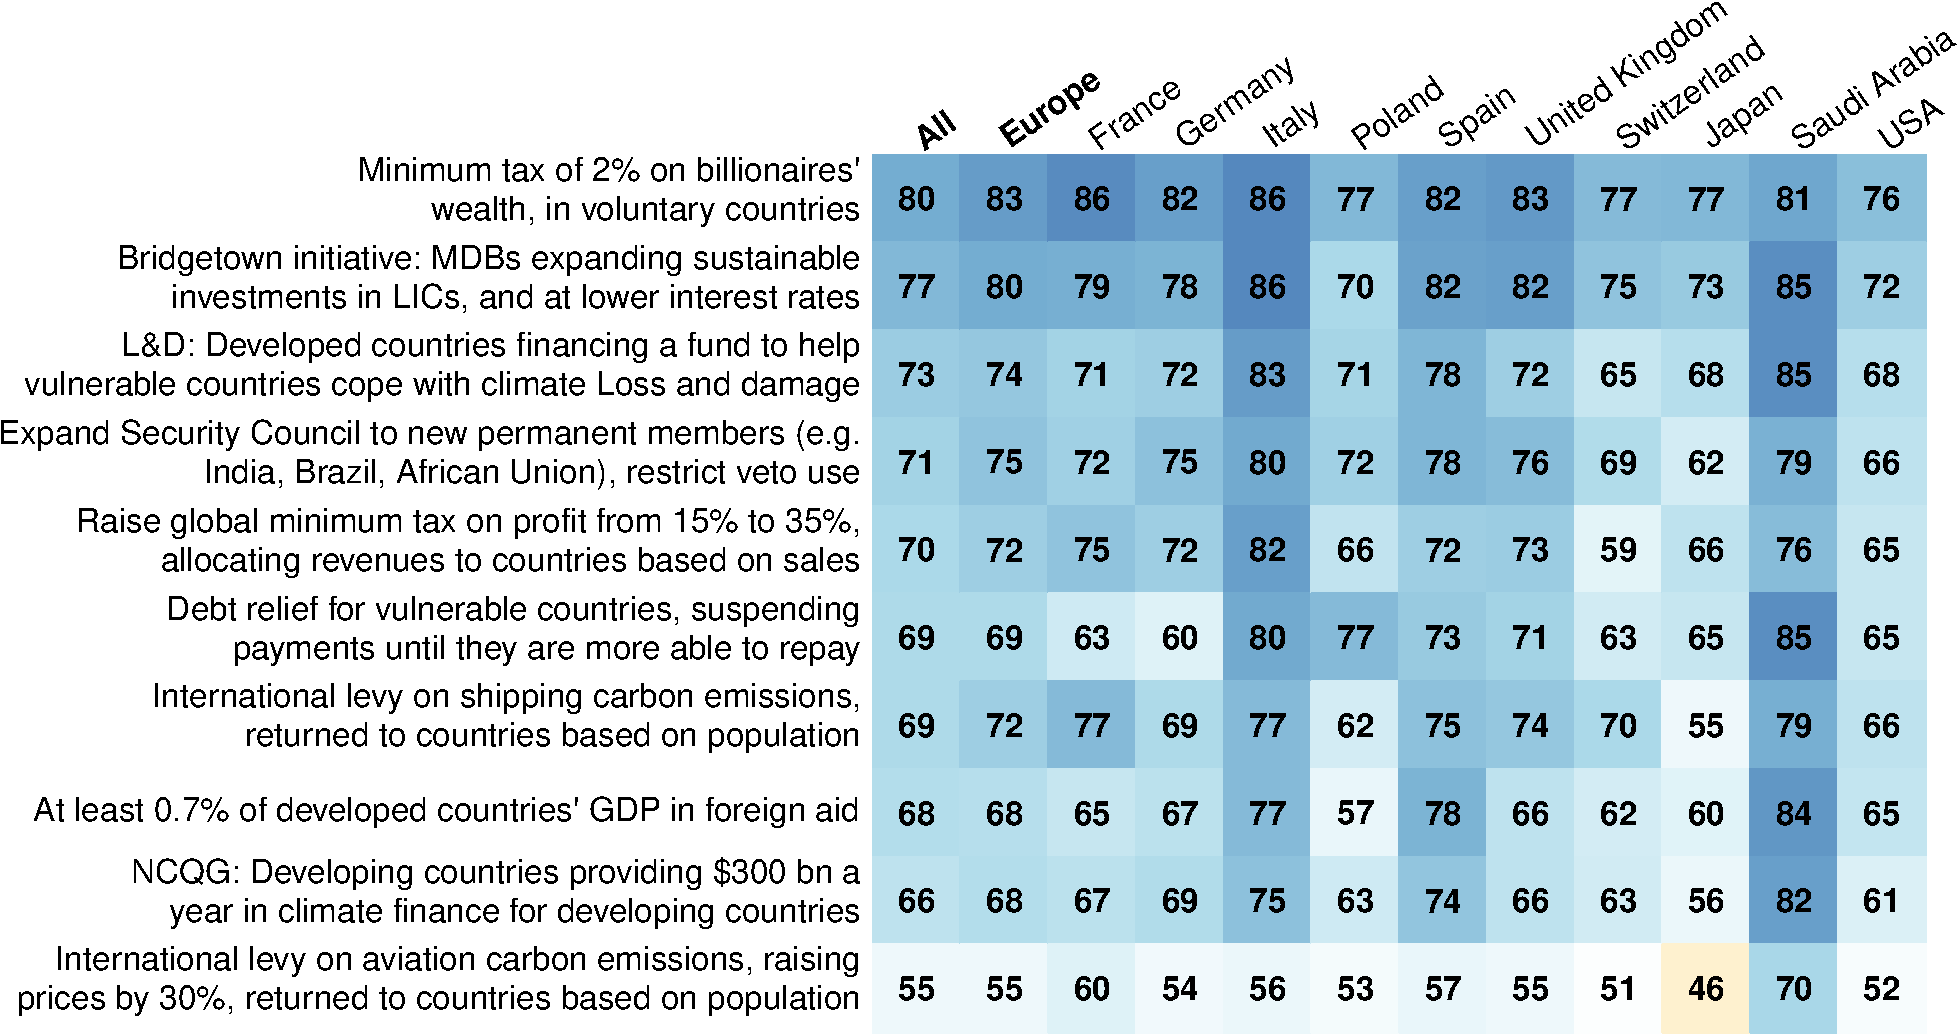
\includegraphics[width=\textwidth]{../figures/country_comparison/solidarity_support_extended_share.pdf}} 
% \end{figure}

% \begin{figure}[H]
%     \caption[{[}Extended sample{]} Support for broad or radical global redistribution]{[Extended sample] Support for broad action or radical proposals of global redistribution. \hfill (Questions~\ref{q:sustainable_future}-\ref{q:top3_tax_support}, \ref{q:convergence_support}-\ref{q:vote_intl_coalition}, \ref{q:reparations_support}, \ref{q:my_tax_global_nation}).
%     }\label{fig:radical_redistr_share_extended} 
%     \makebox[\textwidth][c]{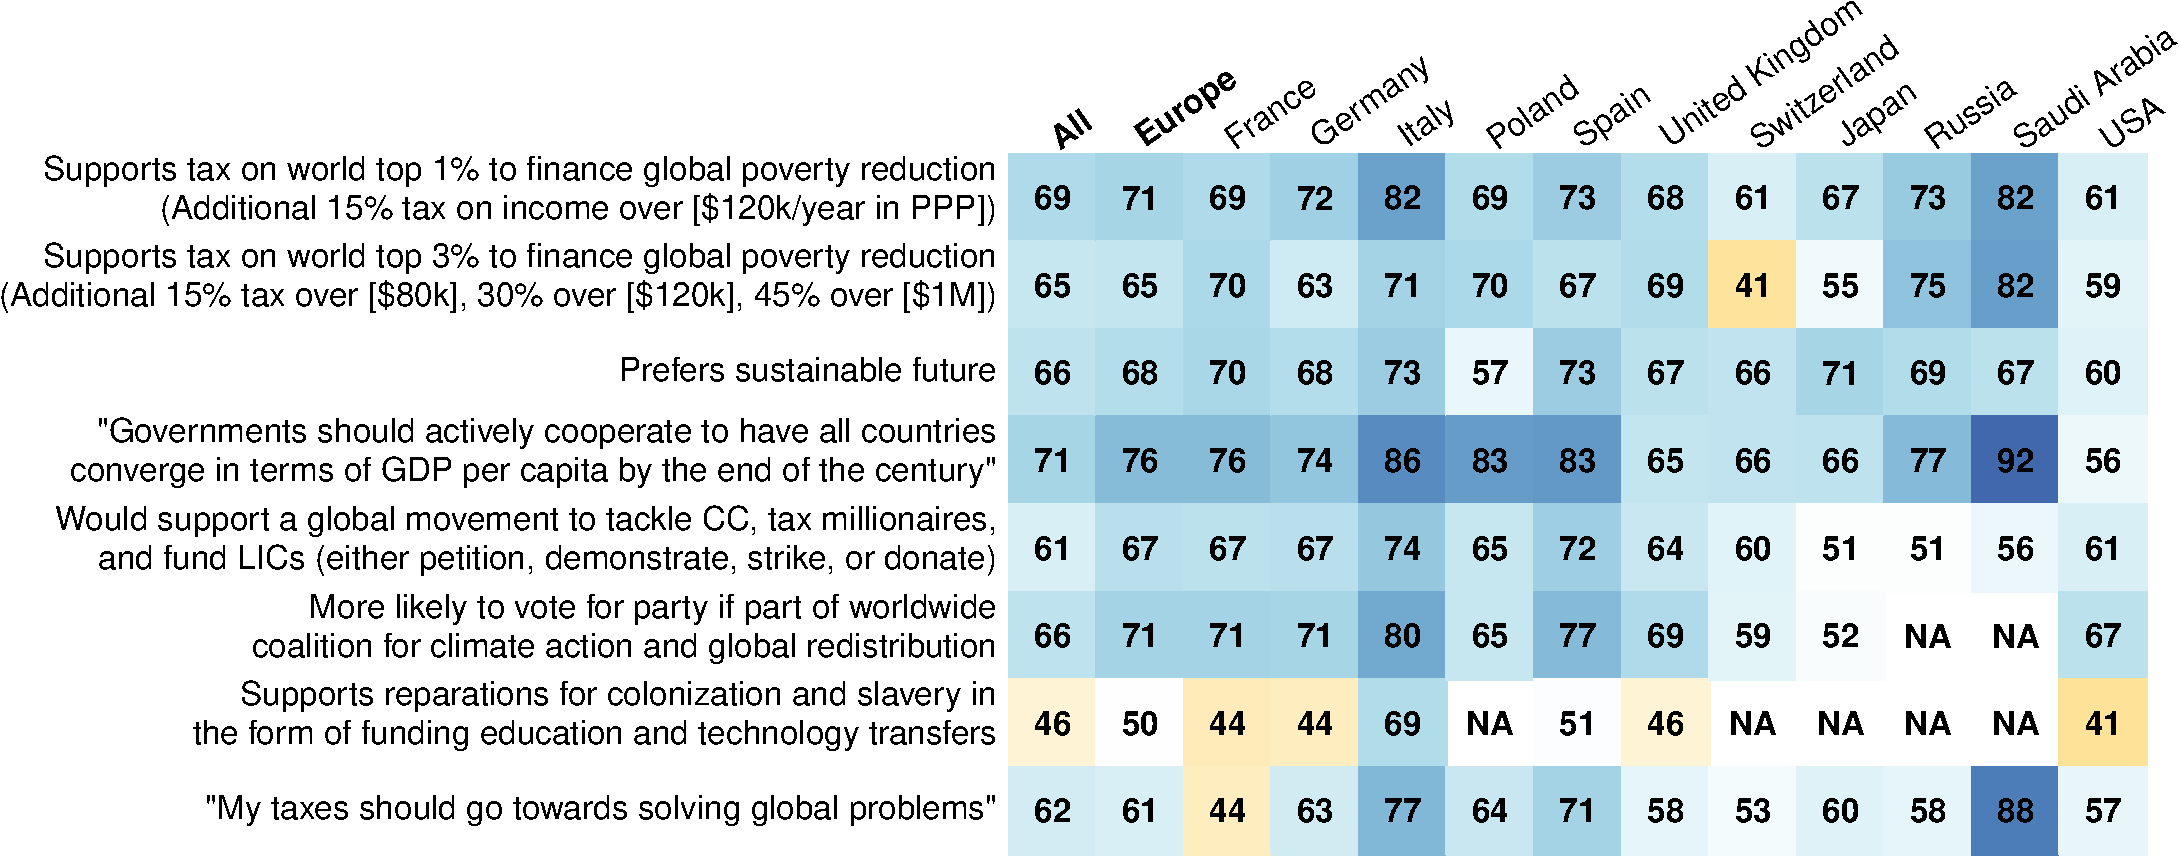
\includegraphics[width=\textwidth]{../figures/country_comparison/radical_redistr_extended_share.pdf}} 
% \end{figure}
% \hfill (Back~to~Section~\ref{par:data_quality}.)

\clearpage
\section{Influence of the Item Order on Answers}\label{app:order}

\begin{table}[!htbp] 
  \caption[Influence of the item order on answers]{Influence of the item order on answers.\hfill (Back~to~Section~\ref{par:data_quality}.)}\label{tab:order} 
  \makebox[\textwidth][c]{\resizebox{.98\paperwidth}{!}{\input{../tables/order.tex}}}
\end{table}

% \clearpage
% \section{Supplementary Tables}\label{app:tables}

% \begin{table}[!htbp] 
%   \caption[Effect of country coverage on support for the ICS]{Support for an International Climate Scheme depending on country coverage.\hfill (Back~to~Section~\ref{subsec:ics}.)}\label{tab:ics} 
%   \makebox[\textwidth][c]{\resizebox{.98\paperwidth}{!}{\input{../tables/ics.tex}}}
%   {\small \textit{Note: Robust standard errors (HC1) are reported in parentheses. \hfill $^{*}$p$<$0.1; $^{**}$p$<$0.05; $^{***}$p$<$0.01.}}
% \end{table}

% \begin{table}[!htbp] 
%   \caption[Effect of country coverage on support for the wealth tax]{Support for an international wealth tax depending on country coverage.\hfill (Back~to~Section~\ref{subsec:wealth_tax}.)}\label{tab:wealth_tax} 
%   \makebox[\textwidth][c]{\resizebox{.98\paperwidth}{!}{\input{../tables/wealth_tax.tex}}}
%   {\small \textit{Note: Robust standard errors (HC1) are reported in parentheses. \hfill $^{*}$p$<$0.1; $^{**}$p$<$0.05; $^{***}$p$<$0.01.}}
% \end{table}

% \begin{table}[!htbp] 
%   \caption[Conjoint analysis: effect of development aid and millionaire tax]{Effect on the likelihood that a political program is preferred of containing the following policies (compared to no foreign policy in the program).\hfill (Back~to~Section~\ref{subsec:conjoint}.)}\label{tab:conjoint} 
%   \makebox[\textwidth][c]{\resizebox{.98\paperwidth}{!}{\input{../tables/conjoint.tex}}}
%   {\small \textit{Note: Robust standard errors (HC1) clustered at the individual levels are reported in parentheses. \hfill $^{*}$p$<$0.1; $^{**}$p$<$0.05; $^{***}$p$<$0.01.}}
% \end{table}

% \begin{table}[!htbp] 
%   \caption[Warm glow: substitute]{Effect of a \textit{Donation lottery} treatment on support for the Global Climate Scheme. (Questions~\ref{q:donation}-\ref{q:gcs_support})\hfill (Back~to~Section~\ref{subsec:warm_glow}.)}\label{tab:warm_glow_substitute} 
%   \makebox[\textwidth][c]{\resizebox{.98\paperwidth}{!}{\input{../tables/warm_glow_substitute.tex}}}
%   {\small \textit{Note: Robust standard errors (HC1) are reported in parentheses. \hfill $^{*}$p$<$0.1; $^{**}$p$<$0.05; $^{***}$p$<$0.01.\\ Control variables (omitted in the table) are: vote, gender, age, income, education, urbanity, likelihood of becoming millionaire, living with partner, employment status, foreign born, country region.}}
% \end{table}

% \begin{table}[!htbp] 
%   \caption[Warm glow: realism]{Effect of information about ongoing global redistribution initiatives on the share of plausible global policies supported. (Questions~\ref{q:info_solidarity}-\ref{q:solidarity_support}).\hfill (Back~to~Section~\ref{subsec:warm_glow}.)}\label{tab:warm_glow_realism} 
%   \makebox[\textwidth][c]{\resizebox{.98\paperwidth}{!}{\input{../tables/warm_glow_realism.tex}}}
%   {\small \textit{Note: Robust standard errors (HC1) are reported in parentheses. \hfill $^{*}$p$<$0.1; $^{**}$p$<$0.05; $^{***}$p$<$0.01. \\ Control variables (omitted in the table) are: vote, gender, age, income, education, urbanity, likelihood of becoming millionaire, living with partner, employment status, foreign born, country region.}}
% \end{table}

% \begin{table}[!htbp] 
%   \caption[Warm glow: IV without control]{Effect on support for global redistribution of believing that it is likely, without control\hfill (Back~to~Section~\ref{subsec:warm_glow}.)}\label{tab:iv_wo_control} 
%   \makebox[\textwidth][c]{\input{../tables/IV_warm_glow_wo_control.tex}} % AER _no_star
%   {\small \textit{Note: Robust standard errors (HC1) are reported in parentheses. \hfill $^{*}$p$<$0.1; $^{**}$p$<$0.05; $^{***}$p$<$0.01.  % AER
%   }}
% \end{table}


% \begin{bibunit}
\clearpage
\listoftables
\listoffigures
\pagestyle{empty}
\renewcommand{\theenumi}{\arabic{enumi}}
\clearpage
\addtocontents{toc}{\protect\setcounter{tocdepth}{0}}
\section*{Questionnaire}\label{app:questionnaire}
\addtocontents{toc}{\protect\setcounter{tocdepth}{3}}
The U.S. version of the questionnaire is presented. Features that vary across countries are placed in square brackets within the question text, as follows: [feature\_name: U.S. value]. The features values for each country are provided in this spreadsheet [anonymized for review]. % APSR
Random branches or conditions for displaying the question are specified in square brackets before the question text (cf. Figure \ref{fig:flow} for the survey flow). The question text is followed by square brackets that refer to Sections, Figures, and Tables presenting the question results, and the variable name(s) corresponding to the question. Finally, response options are displayed in italics. 
Unless otherwise specified, responses are compulsory and a single response much be chosen. %\hfill (Back~to~Section~\ref{par:flow}.)

\subsection*{Welcome} 
 \begin{enumerate} 
\item  \label{q:consent} Welcome to this survey!\\
This survey is \textbf{anonymous }and is conducted \textbf{for research} purposes on a representative sample of [sample\_size: 3,000] [nationality: American people].\\
~\\
It takes around 20 min to complete.\\
~\\
The survey contains lotteries and awards for those who get the correct answer to some comprehension questions.\\
If you are attentive and lucky, \textbf{you can win up to [amount\_lottery: \$100]}.\\
~\\
Please answer every question carefully.\\
~\\
By clicking on the button below, you consent to the terms and conditions.

\end{enumerate} 

 \subsection*{Socio-demographics} 
 \begin{enumerate}[resume] 
\item  \label{q:gender} What is your gender? 
  \\ \textit{Woman; Man; Other}

\item  \label{q:hidden_country} What is your country? 


\item  \label{q:age_exact} What is your age? 
  \\ \textit{Below 18; 18 to 20; 21 to 24; 25 to 29; 30 to 34; 35 to 39; 40 to 44; 45 to 49; 50 to 54; 55 to 59; 60 to 64; 65 to 69; 70 to 74; 75 to 79; 80 to 84; 85 to 89; 90 to 99; 100 or above}

\item  \label{q:foreign} Were you or your parents born in a foreign country?~ 
  \\ \textit{Yes, I was born in a foreign country; Not me but both my parents were born in a foreign country; Not me but one of my parents was born in a foreign country; No, I was born in this country and my parents too}

\item  \label{q:couple} Do you live with your partner (if you have one)? 
  \\ \textit{Yes; No}

\item  \label{q:hh_size} How many people are there in your household? \\The household includes: \textbf{you}, your spouse, \textbf{your family members} who live with you, and your dependents (not flatmates). 
  \\ \textit{1; 2; 3; 4; 5 or more}

\item  \label{q:Nb_children__14} How many children under the age of 14 live with you? 
  \\ \textit{0; 1; 2; 3; 4 or more}

\item ~[new page] \label{q:race} [\textit{Only in: US}] What race or ethnicity do you identify with? (Multiple answers are possible) 
  \\ \textit{White; Black or African American; Hispanic; Asian; American Indian or Alaskan Native; Native Hawaiian or Pacific Islander; Other; Prefer not to say}

\item  \label{q:income} What is the \textbf{[\hyperlink{tab_features}{periodicity\_text}: monthly] [\hyperlink{tab_features}{income\_type}: gross] income of your household}, [income\_type\_long: after taxes and transfers]?

This includes all sources of income: wages, pensions, welfare payments, property income, dividends, self-employment earnings, Social Security benefits, and income from other sources. 
  \\ ~[\textit{All but RU, US}: Custom thresholds, taking into account household composition Questions \ref{q:couple}-\ref{q:Nb_children__14}, and corresponding to the country's deciles and quartiles of standard of living, cf. the sheet ``Income'' in this spreadsheet [anonymized for review]; \\ \textit{RU, US}: Items based on household total income deciles and quartiles, namely in US: \textit{Less than \$17,000; between \$17,001 and \$30,000; between \$30,001 and \$36,000; between \$36,001 and \$43,000; between \$43,001 and \$56,000; between \$56,001 and \$72,000; between \$72,001 and \$91,000; between \$91,001 and \$115,000; between \$115,001 and \$130,000; between \$130,001 and \$150,000; between \$150,001 and \$213,000; More than \$213,000; I prefer not to answer}]  % APSR

\item  \label{q:education} What is your highest completed education level? 
  \\ ~[Country-specific, usually: 0-1 Primary or less; 2 Medium school; 2 Some high school; 3 High school diploma; 3-4 Vocational training; 5 Short-cycle tertiary; 6 Bachelor's; 7-8 Master's or higher]

\item  \label{q:employment_status} What is your employment status? 
  \\ \textit{Full-time employed; Part-time employed; Self-employed; Unemployed (searching for a job); Student; Retired; Inactive (not searching for a job)}

\item  \label{q:zipcode} [\textit{Only the first digits asked in RU, SA}] What is your zipcode?\\
We ask for the zipcode to balance the sample in terms of degree of urbanization (rural, town or city). The survey will be terminated if your zipcode is not recognized. 


\item  \label{q:home} Are you a homeowner or a tenant? (Multiple answers are possible) 
  \\ \textit{Tenant; Owner; Landlord renting out property; Hosted free of charge}

\item ~[new page] \label{q:millionaire} How likely are you to become a millionaire at some point in your life? 
  \\ \textit{Very unlikely; Unlikely; Likely; Very likely; I am already a millionaire}%\footnote{We defined millionaire as having a net wealth of one million dollar or its rounded conversion to Local Currency Unit, except in Poland and Saudi Arabia, where there was a translation mistake (making ``millionaire'' corresponding to a net wealth of \$250,000 in these countries).} revision

\item  \label{q:voted} [\textit{Except in: RU, SA}] Did you vote in the [election: 2024 presidential election]? 
  \\ \textit{Yes; No; Prefer not to say; I didn't have the right to vote in [country\_name: the United States].}

\end{enumerate} 

 \subsection*{Vote} 
 \begin{enumerate}[resume] 
\item  \label{q:nationality_SA} [\textit{Only in: SA}] What is your nationality?\\If you have both the Saudi and a foreign nationality, choose "Saudi". 
  \\ \textit{Saudi; India; Bangladesh; Syria; Yemen; Egypt; Pakistan; Indonesia; Philippines; Sudan; Myanmar; Jordan; Sri Lanka; Nepal; Turkey; Somalia; Lebanon; Other}

\item  \label{q:vote} [\textit{Except in: RU, SA}] [\textit{If voted}: Which candidate did you vote for in the [election: 2024 presidential election]?; \textit{Otherwise}: Even if you did not vote in the [election: 2024 presidential election], please indicate the candidate that you were most likely to have voted for or who represents your views more closely.] 
  \\ ~[Candidates/parties with at least 1\% of votes, e.g. in US: \textit{Harris; Trump; Other; Prefer not to say}. In FR, IT, PL, ES, election is the 2024 European election]

% \item  \label{q:vote_GB} [text\_vote: Which candidate did you vote for in the [election: 2024 European Parliament election]?\\Even if you did not vote in the [election: 2024 European Parliament election], please indicate the candidate that you were most likely to have voted for or who represents your views more closely.] 
%   \\ \textit{Conservative; Labour; Liberal Democrats; SNP; Prefer not to say; Green; DUP; Sinn Féin; Other; Reform UK; Plaid Cymru; Alliance Party of Northern Ireland}

% \item  \label{q:vote_FR} [text\_vote: Which candidate did you vote for in the [election: 2024 European Parliament election]?\\Even if you did not vote in the [election: 2024 European Parliament election], please indicate the candidate that you were most likely to have voted for or who represents your views more closely.] 
%   \\ \textit{Renaissance, MoDem \& Horizons; Rassemblement National; La France insoumise; Les Écologistes – EÉLV; Préfère ne pas répondre; Les Républicains; Résistons (Jean Lassalle); Reconquête; Autre; Parti Socaliste \& Place publique; Parti Communiste Français; Parti animaliste}

% \item  \label{q:vote_CH} [text\_vote: Which candidate did you vote for in the [election: 2024 European Parliament election]?\\Even if you did not vote in the [election: 2024 European Parliament election], please indicate the candidate that you were most likely to have voted for or who represents your views more closely.] 
%   \\ \textit{Social Democratic Party; Swiss People's Party; The Centre; Green Liberal Party; Préfère ne pas répondre; Green Party; Evangelical People's Party; Autre; The Liberals; Federal Democratic Union}

% \item  \label{q:vote_PL} [text\_vote: Which candidate did you vote for in the [election: 2024 European Parliament election]?\\Even if you did not vote in the [election: 2024 European Parliament election], please indicate the candidate that you were most likely to have voted for or who represents your views more closely.] 
%   \\ \textit{United Right (Law and Justice, Sovereign Poland...); Civic Coalition (Civic Platform, Polish Initiative...); Polish People's Party; Prefer not to say; The Left (New Left...); Other; Confederation (New Hope, National Movement, Confederation of the Polish Crown...); Poland 2050}

% \item  \label{q:vote_IT} [text\_vote: Which candidate did you vote for in the [election: 2024 European Parliament election]?\\Even if you did not vote in the [election: 2024 European Parliament election], please indicate the candidate that you were most likely to have voted for or who represents your views more closely.] 
%   \\ \textit{PD; FdI; League; Prefer not to say; SUE; Azione; FI – NM; AVS; PTD; Libertà; M5S; Other}

% \item  \label{q:vote_ES} [text\_vote: Which candidate did you vote for in the [election: 2024 European Parliament election]?\\Even if you did not vote in the [election: 2024 European Parliament election], please indicate the candidate that you were most likely to have voted for or who represents your views more closely.] 
%   \\ \textit{PSOE; PP; Sumar; Prefer not to say; Podemos; Junts UE; Ahora Repúblicas; SALF; CEUS; Vox; Other}

% \item  \label{q:vote_DE} [text\_vote: Which candidate did you vote for in the [election: 2024 European Parliament election]?\\Even if you did not vote in the [election: 2024 European Parliament election], please indicate the candidate that you were most likely to have voted for or who represents your views more closely.] 
%   \\ \textit{AfD; CDU/CSU; BSW; Prefer not to say; Die Linke; FW; Grüne; FDP; Volt; Die Partei; SPD; Other; Tierschutzpartei}

% \item  \label{q:vote_JP} [text\_vote: Which candidate did you vote for in the [election: 2024 European Parliament election]?\\Even if you did not vote in the [election: 2024 European Parliament election], please indicate the candidate that you were most likely to have voted for or who represents your views more closely.] 
%   \\ \textit{CDP; LDP; Reiwa Shinsengumi; Prefer not to say; Sanseitō; CPJ; Komeito; JCP; SDP; Other; Ishin JIP; DPFP}

\end{enumerate} 

 \subsection*{Open-ended field} 
 [\textit{Four random branches}; \textit{Section \ref{subsec:considerations}}]%; Figures \ref{fig:wordcloud}, \ref{fig:field_keyword}-\ref{fig:injustice_field}}; \textit{Random answers can be found on [anonymized for review]}; 
%  \verb|field, variant_field|] 
 \begin{enumerate}[resume] 
\item  \label{q:concerns_field} ~[Branch: concerns] What are your main concerns these days? 


\item  \label{q:wish_field} ~[Branch: wish] What are your needs or wishes? 


\item  \label{q:injustice_field} ~[Branch: injustice] What according to you is the greatest injustice of all?\\ 
~


\item  \label{q:issue_field} ~[Branch: issue] Can you name an issue that is important to you but is neglected in the public debate? 


\end{enumerate} 

 \subsection*{Conjoint analysis} 
 \begin{enumerate}[resume] 
\item  \label{q:conjoint} [\textit{Except in: RU, SA}] Imagine if the two top candidates in your constituency in the next general election campaigned with the following policies in their party's platforms. \\\\Which of these candidates would you vote for?  
~\\

\begin{tabular}{@{\extracolsep{5pt}}|c|c|c|} 
    \hline \\[-1.8ex] 
    \textbf{Candidate A} & \textbf{Candidate B} & \\ \hline \\[-1.8ex]
    ~[Random policy] & [Random policy] & [Policy field in random order] \\ 
    ~[Random policy] & [Random policy] & [Policy field in random order] \\ 
    ~[Random policy] & [Random policy] & [Policy field in random order] \\ 
    ~[Random policy] & [Random policy] & [Policy field in random order] \\ 
    ~[Random policy] & [Random policy] & [Policy field in random order] \\ 
    \hline 
\end{tabular}  

~\\~
  \\ \textit{Candidate A; Candidate B; Neither of them}

\end{enumerate} 

 \subsection*{Revenue split of global tax} 
 [\textit{Two random branches}]%;  \verb|field, variant_split|] 
 \begin{enumerate}[resume] 
\item ~[Branch: Few] \label{q:revenue_split_few} Imagine a wealth tax applied to households with a net worth above [tax\_threshold: \$5 million], implemented in every country around the world.
~\\\\ 
~[tax\_country\_name: In the U.S.], the tax revenues collected would be [\hyperlink{tab_features}{tax\_revenue}: \$514 billion] per year (that is, [\hyperlink{tab_features}{tax\_revenue\_gdp}: 2]\% of [tax\_country\_gdp: U.S. GDP]), while it would be [LIC\_revenue: \$1 billion] in all low-income countries combined (700 million people live in a low-income country, most of them in Africa).
Each country would retain part of the revenues it collects and use it for different domestic purposes. The remaining part would be pooled globally to finance sustainable development in low-income countries.
~\\\\\textbf{What percentage of the global wealth tax revenue should be allocated to each category?} \\\textbf{The total allocation must sum to 100\%.}\\\\ 
~
  \\ \textit{Domestic: Education and Healthcare; Domestic: Social welfare programs; Domestic: Reduction in the federal income tax; Domestic: Reduction of the deficit; Global: Education, Healthcare and Renewable energy in low-income countries}

\item ~[Branch: Many] \label{q:revenue_split_many} Imagine a wealth tax applied to households with net worth above [tax\_threshold: \$5 million], implemented in all countries around the world.
~\\\\ 
~[tax\_country\_name: In the U.S.], the tax revenues collected would be [\hyperlink{tab_features}{tax\_revenue}: \$514 billion] per year (that is, [tax\_revenue\_gdp: 2]\% of [\hyperlink{tab_features}{tax\_country\_gdp}: U.S. GDP]), while it would be [LIC\_revenue: \$1 billion] in all low-income countries combined (700 million people live in a low-income country, most of them in Africa).
Each country would retain part of the revenues it collects and use it for different domestic purposes. The remaining part would be pooled globally to finance sustainable development.
~\\\\\textbf{What percentage of the global wealth tax revenue should be allocated to each category?}~\\\textbf{The total allocation must sum to
100\%.}\\\\ 
~
  \\ ~[Five items are chosen at random among the 13 possible ones: \textit{Domestic: Education and Research; Domestic: Healthcare; Domestic: Defense; Domestic: Deficit reduction; Domestic: Justice and Police; Domestic: Retirement pensions; Domestic: Social welfare programs; Domestic: Infrastructure (public transport, water systems...); Domestic: Income tax reduction; Global: Education and Healthcare in low-income countries; Global: Renewable energy and infrastructure to cope with climate change; Global: Loss and Damage Fund (to rebuild after climate disasters); Global: Forestation and biodiversity projects}]


\end{enumerate} 

 \subsection*{Warm glow -- moral substitute} 
 [\textit{Three random branches: NCS; Donation; control group}]%;  \verb|variant_warm_glow|] 
 \begin{enumerate}[resume] 
\item ~[Branch: NCS] \label{q:ncs_support} Do you agree with the following policy?
~\\
Climate Scheme:~\\
To meet the national climate target, a limited number of permits to emit greenhouse gases would be issued nationally. Polluting firms would be required to buy permits to cover their greenhouse gas emissions. Such a policy would~make fossil fuel companies pay~for their emissions and gradually raise the price of fossil fuels.~Higher prices would encourage people and companies to use less fossil fuels, reducing greenhouse gas emissions.\\
The revenues generated by the sale of permits would finance an equal cash transfer.\textbf{~}Each [country\_adjective: American] would receive [\hyperlink{tab_features}{amount\_expenses}: \$115]per month, thereby offsetting~price increases for the average [country\_adjective: American].\\ 
~\\
\textbf{Do you support the Climate Scheme?} 
  \\ \textit{Yes; No}

\item ~[Branch: Donation] \label{q:donation} By taking this survey, you will be automatically entered into a lottery to win up to [amount\_lottery: \$100]. \\Should you be selected in the lottery, you will have the option to channel a part of this additional compensation to the charity \textit{Just One Tree} to plant trees.\\\\\textbf{In case you win the lottery, what share of the [amount\_lottery: \$100 prize] would you donate to plant trees?} 
  \\ \textit{Share to plant trees}

\end{enumerate} 

 \subsection*{Cap \& Share} 
 \begin{enumerate}[resume] 
\item  \label{q:gcs_support} Do you support the following policy?\\
To ensure that you have attentively read the description,~we will ask some comprehension questions later in the survey: those who get correct answers can win [amount\_lottery: \$100].
~\\
Global Climate Scheme:~\\\\
In 2015, all countries agreed to contain global warming "well below +2~\textdegree{}C". To achieve this,~there is a maximum amount of greenhouse gases we can emit globally.~\\\\
To meet the climate target, a limited number of permits to emit greenhouse gases would be issued globally. Polluting firms would be required to buy permits to cover their greenhouse gas emissions. Such a policy would~make fossil fuel companies pay~for their emissions and gradually raise the price of fossil fuels.~Higher prices would encourage people and companies to use less fossil fuels, reducing greenhouse gas emissions.\\\\
In accordance with the principle that each human has an equal right to pollute, the revenues generated by the sale of permits could finance a global basic income.~Every adult would receive [\hyperlink{tab_features}{amount\_bi}: \$35]per month, thereby lifting 600 million people who earn less than \$2 a day out of extreme poverty.\\
The typical [national: American] would lose out financially [\hyperlink{tab_features}{amount\_lost}: \$90]per month~(as he or she would face around [\hyperlink{tab_features}{price\_increase}: 2]\% in price increases, which is higher than the [\hyperlink{tab_features}{amount\_bi}: \$35]per month they would receive).\\\\
The policy could be implemented as soon as 100 countries agree to it. Countries that would refuse to take part in the policy could face sanctions (like tariffs) from the rest of the world and would be excluded from the basic income program.\\\\
~\\\textbf{
Do you support the Global Climate Scheme?
} 
  \\ \textit{Yes; No}\\\\
~[new page] [\textit{Two random branches: own; US}]%; \textit{Figure \ref{fig:ncs_gcs_ics}}; \verb|gcs_belief, variant_belief|] 
\item ~[Branch: US] \label{q:gcs_belief_us} According to you, \textbf{what percentage of [belief\_nationality: \textit{All but US: Americans; US: Europeans}] would answer \textit{Yes }to the previous question} (considering that typical [belief\_nationality] would lose [belief\_loss: \$140] per month from the Global Climate Scheme)\textbf{?}\\ The respondent who is closest to the correct value will get [amount\_lottery: \$100]. %
  \\ \textit{Percentage of [belief\_nationality] in favor of Global Climate Scheme}

\item ~[Branch: own] \label{q:gcs_belief_own} According to you, \textbf{what percentage of \textit{[nationality: fellow citizens]} would answer \textit{Yes }to the previous question?}\\ The respondent who is closest to the correct value will get [amount\_lottery: \$100]. %
  \\ \textit{Percentage of [nationality: fellow citizens] in favor of Global Climate Scheme}

\end{enumerate} 

 \subsection*{Cap \& Share non-universal} 
 ~[\textit{Four random branches: low; mid; high; high\_color}; \textit{Section \ref{subsec:ics}}]%; Figures \ref{fig:ics}, \ref{fig:ncs_gcs_ics}}; 
%  \verb|ics_support|] 
 \begin{enumerate}[resume] 
\item ~[Branch: low]  \label{q:gcs_low} Below is a map showing a possible set of countries that would participate in the Global Climate Scheme previously described.\\
~\\
These countries include India, the European Union, as well as all Africa, Latin America, South-Asia and South-East Asia.\\
Collectively, these [nb\_countries\_low: 145] countries account for [emissions\_low\_without: 40]\% of global emissions (if [ics\_country: the U.S.] joined them, [emissions\_low\_with: 40]\% of global emissions would be covered).\\
~\\ 

\item ~[Branch: mid] \label{q:gcs_mid} Below is a map showing a possible set of countries that would participate in the Global Climate Scheme previously described.\\
~\\
These countries include China, India, as well as all Africa, Latin America, South-Asia and South-East Asia.\\
Collectively, these 119 countries account for 56\% of global emissions (if [ics\_country: the U.S.] joined them, [emissions\_mid\_with: 70]\% of global emissions would be covered).\\
~\\ 

\item ~[Branch: high]  \label{q:gcs_high} Below is a map showing a possible set of countries that would participate in the Global Climate Scheme previously described.\\
~\\
These countries include China, India, [text\_countries\_high: the European Union, Japan, the United Kingdom], Canada, South Korea, as well as all Africa, Latin America, South-Asia and South-East Asia.~\\
Collectively, these [nb\_countries\_high: 153] countries account for [emissions\_high\_without: 71]\% of global emissions (if [ics\_country: the U.S.] joined them, [emissions\_high\_with: 86]\% of global emissions would be covered).\\
~\\ 

\item ~[Branch: high\_color]  \label{q:gcs_high_color} Below is a map showing a possible set of countries that would participate in the Global Climate Scheme previously described.\\
~\\
These countries include China, India, [text\_countries\_high: the European Union, Japan, the United Kingdom], Canada, South Korea, as well as all Africa, Latin America, South-Asia and South-East Asia. \\
Collectively, these [nb\_countries\_high: 153] countries account for [emissions\_high\_without: 72]\% of global emissions (if [ics\_country: the U.S.] joined them, [emissions\_high\_with: 86]\% of global emissions would be covered).\\\\Note that a provision would prevent the Global Climate Scheme from harming low- and middle-income countries: this is why countries like China, Mexico, or Egypt are in white on the map (they would neither win nor lose financially).\\


\item  \label{q:ics_support} Do you support [ics\_country: the U.S.] joining the Global Climate Scheme, in case it is adopted by the above countries? 
  \\ \textit{Yes; No}

\end{enumerate} 

 \subsection*{Warm glow -- realism} 
 \begin{enumerate}[resume] 
\item ~[\textit{Two random branches: with or without this informational text.}] \label{q:info_solidarity} To ensure that you have attentively read the description below, we will ask some comprehension questions later in the survey: those who get correct answers can win \$100.

~\\\\In several international organizations, \textbf{countries have agreed to demonstrate some degree of solidarity in addressing global challenges}.\\
Negotiations are ongoing to implement specific mechanisms for sustainable development.\\\\Here are a few examples:\\🚢~In 2025, to reduce carbon emissions from shipping, \textbf{the International Maritime Organization adopted an international levy on excess emissions from maritime fuel, that should partly finance low-income countries}.\\📦~Since 1970, \textbf{developed countries have agreed to contribute 0.7\% of their GDP in foreign aid} and development assistance.\\
🌱 In international climate negotiations, \textbf{developed countries have committed to finance climate action in developing countries}. In 2009, they committed to provide \$100 billion per year by 2020. In 2023, all countries agreed to set up a fund to help vulnerable countries cope with loss and damage from climate change. In 2024, the \$100 billion goal was increased to \$300 billion per year by 2035.\\📈~In 2021, 136 countries adopted a minimum tax rate of 15\% on multinational profits.\\💎 In 2024, under the leadership of Brazil, \textbf{the G20 considered the introduction of a global tax} of 2\% \textbf{on }the wealth of \textbf{billionaires}.
~\\🌐~In 2024, the UN General Assembly adopted the Pact for the Future, which foresees a reform of the UN Security Council to limit the power of its five permanent member and expand it to new members.\\🔄 Led by the Prime Minister of Barbados and supported by the UN Secretary General, the Bridgetown initiative seeks a new financial system that would drive financial resources towards climate action and sustainable development. 


\item  \label{q:likely_solidarity} According to you, how likely is it that international policies involving significant transfers from high-income countries to low-income countries will be introduced in the next 15 years? 
  \\ \textit{Very unlikely; Unlikely; Likely; Very likely}

\item  \label{q:solidarity_support} Do you support or oppose the following policies?\\
~\\ 
~[\textit{Only in PL, SA}: (As some items refer to ``developed countries'', note that we consider [Saudi Arabia] to be a developed country in this question.)]  \\
~[Item order is randomized]
\begin{itemize}
    \item Institutions like the World Bank investing in many more sustainable projects in lower-income countries, and offering lower interest rates (the Bridgetown initiative)
    \item Developed countries financing a fund to help vulnerable countries cope with loss and damage from climate change
    \item Expanding the UN Security Council (in charge of peacekeeping) to new permanent members such as India, Brazil, and the African Union, and restricting the use of the veto\footnote{In Russia, due to a mistake in the questionnaire, this item was not asked to the control group. Therefore, results are based on the treated group for this item in Russia. }
    \item Raising the globally agreed minimum tax rate on profits of multinational firms from 15\% to 35\%, closing loopholes and allocating revenues to countries where sales are made
    \item Debt relief for vulnerable countries by suspending repayments until they are better able to repay, promoting their development
    \item An international levy on carbon emissions from shipping, funding national budgets in proportion to population
    \item An international levy on carbon emissions from aviation, raising ticket prices by 30\% and funding national budgets in proportion to population
    \item Developed countries providing \$300 billion a year (0.4\% of their GDP) to finance climate action in developing countries
    \item Developed countries contributing at least 0.7\% of their GDP in foreign aid and development assistance
    \item A minimum tax of 2\% on the wealth of billionaires, in voluntary countries
\end{itemize}
\textit{Strongly oppose; Somewhat oppose; Indifferent; Somewhat support; Strongly support}
\end{enumerate} 

 \subsection*{NCQG} 
 [\textit{Two random branches: Full; Short}]%; %\textit{Figure \ref{fig:field}}; 
%  \verb|ncqg_fusion, variant_ncqg|] 
 \begin{enumerate}[resume] 
% \item  \label{q:maritime_split} This year, to meet the global climate targets, the International Maritime Organization is designing a global levy on shipping carbon emissions.\\\\\textbf{According to you, what percentage of the revenue from a maritime fuel levy should be allocated to each category below?} The total must be 100\%.\\ 
% ~
%   \\ \textit{Fostering sustainable transition in the least developed countries and small islands states; Return revenues to shipping companies to prevent increases in shipping costs; Finance research, development and deployment for zero-emission fuels and ships}

\item ~[Branch: Full] \label{q:ncqg_full} \textbf{At international climate negotiations, developing countries call for larger provision of "climate finance": the financing of climate action from developed countries in developing countries.} [developed\_note: (Note that we consider Saudi Arabia to be a developed country in this question.)]\\\\\textbf{There are two kinds of climate finance: grants (that is, donations) and loans. In 2022, \$26 billion was provided as grants and the rest as loans, for a total of \$116 billion.~}\\\\In 2009, developed countries agreed to mobilize \$100 billion per year in climate finance by 2020. In 2024, they committed to raise this goal to \$300 billion by 2035. None of the goals specify which share should be provided as grants.\\\\Below are different positions on the amount of climate finance that should be provided in 2035, all expressed in grant-equivalent terms (that is, not counting loans):\\-~ ~ ~ ~ \$0: There should be no contributions from developed countries to climate action in developing countries.\\-~ ~ ~ \$26 billion (0.04\% of developed countries' GDP): The current amount, consistent with the old (2020) goal.\\-~ ~ \$100 billion (0.14\% of GDP): The old (2020) goal, if all climate finance were provided as grants.\\-~ ~ \$300 billion (0.43\% of GDP): The new (2035) goal, if all climate finance were provided as grants.\\-~ ~ \$600 billion (0.86\% of GDP):~The goal called for by India, a position shared by most developing countries.\\- \$1,000 billion (1.43\% of GDP): The goal called for by Climate Action Network (a network of NGOs including Greenpeace, Oxfam, and WWF).\\- \$5,000 billion (7.14\% of GDP): The goal called for by Demand Climate Justice (a network of NGOs including 350.org and~the World Council of Churches)\\\\\textbf{If you could choose the amount of climate finance provided by developed countries to developing countries in 2035, what amount would you choose (in grant-equivalent terms)?}\\ 
~\\
~[Item order is randomly reversed or not]
  \\ \textit{\$0; \$26 billion; \$100 billion; \$300 billion; \$600 billion; \$1,000 billion; \$5,000 billion}

\item ~[Branch: Short] \label{q:ncqg} \textbf{"Climate finance" designates the financing of climate action from developed countries in developing countries.} [developed\_note: (Note that we consider Saudi Arabia to be a developed country in this question.)]\\\\\textbf{There are two kinds of climate finance: grants (that is, donations) and loans. The large majority is currently provided as loans.~}\\\\In 2009, developed countries agreed to mobilize \$100 billion per year in climate finance. In 2024, they committed to triple this goal by 2035. None of the goals specify which share should be provided as grants.~\\At international climate negotiations, developing countries call for larger provision of climate finance, particularly in the form of grants.\\\\\textbf{If you could choose the level of climate finance provided by developed countries to developing countries in 2035, what would you choose?}\\ 
~\\
~[Item order is randomly flipped or not]
  \\ \textit{Stop all provision of climate finance.; \\Reduce the provision of climate finance.; \\Maintain current contributions (\$26 billion per year in grants, that is 0.04\% of developed countries' GDP, and \$80 billion in loans, or 0.1\% of GDP).; \\ Meet the newly agreed goal by tripling grants and loans (\$100 billion in grants, or 0.15\% of GDP).; \\ Increase climate finance to a level between what developed countries have agreed and what developing countries are asking for (\$300 billion in grants, or 0.45\% of GDP).; \\Increase climate finance to match what developing countries are asking for (\$600 billion in grants, or 0.9\% of GDP).; \\Increase climate finance to match what NGOs are asking for (at least \$1,000 billion per year in grants, that is 1.4\% of GDP, is what Greenpeace, Oxfam, WWF, and the World Council of Churches ask for).}

\end{enumerate} 

 \subsection*{Wealth tax depending on sets of countries} 
 [\textit{Three random branches: Global; HIC; Int'l}] %; \textit{Section \ref{subsec:wealth_tax}; Figures \ref{fig:wealth_tax}, \ref{fig:wealth_tax_heatmap}}; 
%  \verb|wealth_tax_support|] 
 \begin{enumerate}[resume] % TODO: plus condensé ?
\item ~[Branch: Global] \label{q:global_tax_support} \textbf{Imagine an international tax on individuals with net worth above [wealth\_threshold: \$1 million].~}\\Only wealth above [wealth\_threshold: \$1 million] would be taxed, at a rate of 2\%. Each country would retain 70\% of the revenues it collects, while 30\% would be pooled at the global level to finance public services in low-income countries (in particular, access to drinking water, healthcare, and education in Africa). \\\\Say we are in 2030. \textbf{Imagine that all other countries in the world adopt this policy. \\Do you support [country\_name: the United States] adopting this international tax on millionaires?}
  \\ \textit{Yes; No}

\item ~[Branch: HIC] \label{q:hic_tax_support} \textbf{Imagine an international tax on individuals with net worth above [wealth\_threshold: \$1 million].~}\\Only wealth above [wealth\_threshold: \$1 million] would be taxed, at a rate of 2\%. Each country would retain 70\% of the revenues it collects, while 30\% would be pooled at the global level to finance public services in low-income countries (in particular, access to drinking water, healthcare, and education in Africa). \\\\Say we are in 2030. \textbf{[hic\_tax: Imagine that all other high-income countries (such as the European Union, Japan, and Canada) adopt this policy and some middle-income countries (such as China) do not.]}\textbf{~\\Do you support [country\_name: the United States] adopting this international tax on millionaires?}
  \\ \textit{Yes; No}

\item ~[Branch: Int'l] \label{q:intl_tax_support} \textbf{Imagine an international tax on individuals with net worth above [wealth\_threshold: \$1 million].~}\\Only wealth above [wealth\_threshold: \$1 million] would be taxed, at a rate of 2\%. Each country would retain 70\% of the revenues it collects, while 30\% would be pooled at the global level to finance public services in low-income countries (in particular, access to drinking water, healthcare, and education in Africa). \\\\Say we are in 2030.\textbf{ [intl\_tax:\footnote{Excluded countries are \textit{China, Japan, and Canada}. As for included countries, on top of \textit{Brazil}, they are: \textit{the EU and the UK} for Switzerland, Saudi Arabia, and the U.S.; the EU\textit{} for Russia and the UK; and \textit{France, Germany, Spain, and the UK (except one's own country)} for EU countries.} Imagine that some countries  (such as the European Union) adopt this policy and others (such as Japan, Canada, and China) do not.]\\Do you support [country\_name: the United States] adopting this international tax on millionaires?}
  \\ \textit{Yes; No}

\end{enumerate} 

 \subsection*{Scenarios \& radical tax} 
 [\textit{Scenario A \& B are randomly interverted.}]
 \begin{enumerate}[resume] 
\item  \label{q:sustainable_future} \textbf{Consider two possible scenarios for the world for the next 20 years.~\\\\Scenario A}: \\Most countries implement coordinated policies to limit global warming to +2\textdegree{}C and reduce inequality. The world greatly reduces greenhouse gas emissions and is on track to meet its climate target. Taxes on millionaires fund the installation of heat pumps, the thermal insulation of buildings, and improved public transportation. Yachts and private jets are phased out worldwide. Cars are all electric by 2045, and they are about the same price as internal combustion cars nowadays. By 2045, environmental regulations gradually double the price heating fuel or gas, air travel, and beef. As a result, people fly half as much, eat half as much meat, and use more public transportation in 2045 than they did in 2025. Despite higher prices for polluting goods, the overall purchasing power is preserved, thanks to a decrease in sales tax that reduces the prices of non-polluting goods.\\\\\textbf{Scenario B}:\\Since 2025, no additional policies are implemented to address climate change or inequality. People maintain the same lifestyles as in 2025. For example, most people continue to drive cars with internal combustion engines. Greenhouse gas emissions are stable. Global warming is expected to reach +3\textdegree{}C by 2100 and higher levels beyond that date. A warmer climate will cause more frequent and more severe droughts, heatwaves, wildfires, and floodings.\\\\Apart from the elements described, the two scenarios are the same (for example, in terms of unemployment or crime). \\\\\textbf{Which scenario do you prefer for the future?} 
  \\ \textit{Scenario A; Scenario B} \\\\
% \item  \label{q:sustainable_future_b} \textbf{Consider two possible scenarios for the world for the next 20 years.~\\\\Scenario A}:\\Since 2025, no additional policies are implemented to address climate change or inequality. People maintain the same lifestyles as in 2025. For example, most people continue to drive cars with internal combustion engines. Greenhouse gas emissions are stable. Global warming is expected to reach +3\textdegree{}C by 2100 and higher levels beyond that date. A warmer climate will cause more frequent and more severe droughts, heatwaves, wildfires, and floodings.\\\\\textbf{Scenario B}: \\Most countries implement coordinated policies to limit global warming to +2\textdegree{}C and reduce inequality. The world greatly reduces greenhouse gas emissions and is on track to meet its climate target. Taxes on millionaires fund the installation of heat pumps, the thermal insulation of buildings, and improved public transportation. Yachts and private jets are phased out worldwide. Cars are all electric by 2045, and they are about the same price as internal combustion cars nowadays. By 2045, environmental regulations gradually double the price of heating fuel or gas, air travel, and beef. As a result, people fly half as much, eat half as much meat, and use more public transportation in 2045 than they did in 2025. Despite higher prices for polluting goods, the overall purchasing power is preserved, thanks to a decrease in sales tax that reduces the prices of non-polluting goods.\\\\Apart from the elements described, the two scenarios are the same (for example, in terms of unemployment or crime). \\\\\textbf{Which scenario do you prefer for the future?} 
%   \\ \textit{Scenario A; Scenario B}
  ~[new page] [\textit{Two random branches: top1; top3}; \textit{Section \ref{par:global_income_redistr}}]%; Figures \ref{fig:radical_redistr_share}, \ref{fig:top_tax_share}-\ref{fig:top_tax_positive}}; 
% \verb|top_tax_support|, \verb|variant_top_tax|]
\item ~[Branch: top1] \label{q:top1_tax_support} Currently, 2 billion people live in acute poverty, with less than [lcu\_250: \$250][periodicity: per month].\\The Sustainable Development Goals, adopted by all countries in 2015, aim to alleviate poverty and give access to healthcare, education, drinking water, and sanitation for all by 2030.~Due to lack of funding, the world is not on track to meet these poverty reduction goals.\\\\\textbf{Poverty reduction could be funded by a global tax on individual income above [\hyperlink{tab_features}{lcu\_120k}: \$120,000][\hyperlink{tab_features}{periodicity\_tax}: per year].~\\The tax rate would be 15\% for every [currency: dollar] over [lcu\_120k: \$120,000] of income} after existing taxes.~\\For example, a single person earning [lcu\_130k: \$130,000][periodicity\_tax: per year] after taxes would pay [lcu\_1500: \$1,500] in additional taxes, or 15\% of [lcu\_10k: \$10,000] = [lcu\_130k: \$130,000]~$-$~[lcu\_120k: \$120,000]. Meanwhile, a married couple earning [lcu\_200k: \$200,000][periodicity\_tax: per year], [lcu\_100k: \$100,000] for each of them, would go untaxed.\\This tax would apply to the richest 1\% of the world's population. [tax\_country\_name: In the United States], it would affect the richest [affected\_top1: 8]\% and redistribute [transfer\_top1: 3]\% of GDP to lower-income countries.\\\\\textbf{Do you support or oppose such a global tax on the richest people to finance global poverty reduction?}\\ 
  \\ \textit{Strongly oppose; Somewhat support; Strongly support; Somewhat oppose; Indifferent}

\item ~[Branch: top3] \label{q:top3_tax_support} Currently, 3 billion people live in deep poverty, with less than [lcu\_400: \$400][periodicity: per month].\\The Sustainable Development Goals, adopted by all countries in 2015, aim to alleviate poverty and achieve access to healthcare, education, drinking water, and sanitation for all by 2030.~Due to lack of funding, the world is not on track to meet these poverty reduction goals.\\\\\textbf{Poverty reduction could be funded by a global tax on individual income above [\hyperlink{tab_features}{lcu\_80k}: \$80,000][\hyperlink{tab_features}{periodicity\_tax}: per year].~\\The tax rate would be 15\% for every [currency: dollar] over [lcu\_80k: \$80,000] of income} after existing taxes, \textbf{30\% over [\hyperlink{tab_features}{lcu\_120k}: \$120,000], and 45\% over [\hyperlink{tab_features}{lcu\_1M}: \$1 million].~}\\For example, a single person earning [lcu\_90k: \$90,000][periodicity\_tax: per year] after taxes would pay [lcu\_1500\_top3: \$1,500] in additional taxes, or 15\% of [lcu\_10k\_top3: \$10,000] = [lcu\_90k: \$90,000]~$-$~[lcu\_80k: \$80,000]. Meanwhile, a married couple earning [lcu\_150k: \$150,000][periodicity\_tax: per year], [lcu\_75k: \$75,000] for each of them, would go untaxed.\\This tax would apply to the richest 3\% of the world's population. [tax\_country\_name: In the United States], it would affect the richest [affected\_top3: 18]\% and redistribute [transfer\_top3: 8]\% of GDP to lower-income countries.\\\\\textbf{Do you support or oppose such a global tax on the richest people to finance global poverty reduction?}\\ 
~
  \\ \textit{Strongly oppose; Somewhat support; Strongly support; Somewhat oppose; Indifferent}

\item  \label{q:attention_test} To show that you are attentive, please select "A little" in the following list: 
  \\ \textit{Not at all; A little; A lot; A great deal}

\end{enumerate} 

 \subsection*{Preferred transfer means to LICs} 
 \begin{enumerate}[resume] 
\item  \label{q:transfer_how} Below are different ways to transfer resources to help reduce poverty in a low-income country.~\\How do you evaluate each of these options?\\ 
~
~[Item order is randomly flipped or not]
\begin{itemize}
  \item Transfers to public development aid agencies which then finance suitable projects
  \item Transfers to the national government conditioned on the use of funds for poverty reduction programs
  \item Unconditional transfers to the national government
  \item Unconditional transfers to local authorities (municipality, village chief...)
  \item Transfers to local NGOs with democratic decision-making processes
  \item Cash transfers to parents (child allowances), to the disabled and to the elderly
  \item Unconditional cash transfers to each household
\end{itemize}
\textit{A wrong way; An acceptable way; A right way; The best way}

\end{enumerate} 

 \subsection*{Radical redistribution} 
 \begin{enumerate}[resume] 
\item  \label{q:convergence_support} Should governments actively cooperate to have all countries converge in terms of GDP per capita by the end of the century? 
  \\ \textit{Yes; No; I prefer not to answer}

\item  \label{q:global_movement} If there was a worldwide movement in favor of a global program to tackle climate change, implement taxes on millionaires and fund poverty reduction in low-income countries, to what extent would you be willing to be part of that movement? (Multiple answers possible) 
  \\ \textit{I would \textit{not} support such a movement.; I could sign a petition and spread ideas.; I could attend a demonstration.; I could go on strike.; I could donate [amount\_lottery: \$100] to a strike fund.}

\item ~[\textit{Except in: RU, SA}] \label{q:vote_intl_coalition} Let us call "your political party" the party you voted for in the last election, or the party that represents your views most closely.~\\\textbf{Imagine }there was \textbf{a worldwide coalition} of political parties in favor of a common program \textbf{to tackle climate change, implement taxes on millionaires and fund poverty reduction in low-income countries}.~\\\\\textbf{Would you be more likely 
to vote for your party if it were part of that coalition?}\\ 
~
~[Item order is randomly flipped or not]
  \\ \textit{Yes, I would be \textbf{more likely} to vote for my party if it joined that coalition (or to vote for another party if only that other party joined the coalition).; \\My choice would \textbf{not depend} on which parties are part of that coalition.; \\No, I would be \textbf{less likely} to vote for my party if it joined that coalition.}

\item  \label{q:why_hic_help_lic} Some people think that high-income countries should support low-income countries.~\\Among the different reasons given, which ones do you agree with? (Multiple answers possible) 
~[Order of the first three items is randomized]
  \\ \textit{High-income countries have a historical responsibility for the current situation in low-income countries.; \\In the long run, it is in the interest of high-income countries to help low-income countries.; \\Helping those in need is the right thing to do. This is also true at the international level.; \\None of the above.}

\item ~[\textit{Only in: FR, DE, IT, ES, GB, US}] \label{q:reparations_support} Some people argue that Western countries owe reparations for colonization and slavery to former colonies and descendants of slaves. \\Reparations could take the form of funding education and facilitating technology transfers, to address unequal opportunities passed down from the past. \\\\\textbf{Do you support or oppose reparations} of this kind \textbf{for colonization and slavery?~}\\ 
~
  \\ \textit{Strongly oppose; Somewhat oppose; Indifferent; Somewhat support; Strongly support}

\end{enumerate} 

 \subsection*{[\textit{Except in: RU}] Custom redistribution} 
 \begin{enumerate}[resume] 
\item \label{q:income_exact} What is the \textit{[\hyperlink{tab_features}{periodicity\_text}: yearly]} income of your household \textbf{after taxes and social benefits}?\\This includes all sources of income: salaries, pensions, allowances, welfare benefits, property income, etc.\\My household earns ... [text\_unit: \$ per year] (answer with no comma, no space, no period):\\ 
~

\item ~[new page] \label{q:custom_redistr} If you could redistribute income at the global level, what would you do? In this question, we let you choose your preferred parameters for a redistribution of income at the world level.~\\If you prefer to skip this question, check the corresponding box at the bottom of the page.\\\\The worldwide redistribution of income would take the form of additional policies, taxes, and transfers, on top of existing ones.\\These policies would lower the income of the richest (the losers from the redistribution) and increase the income of the poorest (the winners).~\\\\Below you will find a graph of the world distribution of after-tax income and three sliders that vary it. The current distribution is in red, and your custom one is in green.~\\The first two sliders~control the proportion of winners and the proportion of losers, among all humans. The third slider controls the degree of redistribution from the richest to the poorest.~\\If you do not want new policies to reduce global inequality, you can set the third slider to zero.~\\\\\textbf{You need to move the sliders} (by holding the mouse down on the little squares and moving to the side) to make the green curve evolve: the idea is to move the sliders \textbf{until you get a green curve you are satisfied with}. \\\\

~\\Examples of income changes after your proposed redistribution:\\

\begin{tabular}{@{\extracolsep{5pt}}|c|c|} 
    \hline \\[-1.8ex] 
    \textbf{Now} & \textbf{After} \\\hline %\\[-1.8ex]
    0 [text\_unit: \$ per year] & [after\_0] [text\_unit: \$ per year] \\ 
    ~[now\_10k] [text\_unit] & [after\_10k] [text\_unit] \\ 
    ~[now\_60k] [text\_unit] & [after\_60k] [text\_unit] \\ 
    ~[now\_100k] [text\_unit] & [after\_100k] [text\_unit] \\ 
    \multicolumn{2}{c}{Your \textit{individual} income} \\ 
    ~[own] [text\_unit] & [after\_own] [text\_unit] \\ 
    \hline 
\end{tabular}  

\textit{I am satisfied with my custom redistribution.; \\I want to skip this question.}

\end{enumerate} 

 \subsection*{Well-being (\textit{for another project})} 
  [\textit{Four random branches: gallup\_0; gallup\_1; wvs\_0; wvs\_1}]%; %\textit{Figure \ref{fig:well_being}}; 
%  \verb|well_being, variant_well_being|] 
 \begin{enumerate}[resume] % TODO? condenser?
\item ~[Branch: gallup\_0] \label{q:well_being_gallup_0} Please imagine a ladder, with steps numbered from 0 at the bottom to 10 at the top. The top of the ladder represents the best possible life for you and the bottom of the ladder represents the worst possible life for you. \\\\On which step of the ladder would you say you personally feel you stand at this time? 
  \\ \textit{Worst possible 0; 1; 2; 3; 4; 5; 6; 7; 8; 9; Best possible 10}

\item ~[Branch: gallup\_1] \label{q:well_being_gallup_1} Please imagine a ladder, with steps numbered from 1 at the bottom to 10 at the top. The top of the ladder represents the best possible life for you and the bottom of the ladder represents the worst possible life for you. \\\\On which step of the ladder would you say you personally feel you stand at this time? 
  \\ \textit{Worst possible 1; 2; 3; 4; 5; 6; 7; 8; 9; Best possible 10}

\item ~[Branch: wvs\_0] \label{q:well_being_wvs_0} All things considered, how satisfied are you with your life as a whole these days? 
  \\ \textit{Completely dissatisfied 0; 1; 2; 3; 4; 5; 6; 7; 8; 9; Completely satisfied 10}

\item ~[Branch: wvs\_1] \label{q:well_being_wvs_1} All things considered, how satisfied are you with your life as a whole these days? 
  \\ \textit{Completely dissatisfied 1; 2; 3; 4; 5; 6; 7; 8; 9; Completely satisfied 10}

\end{enumerate} 

 \subsection*{Comprehension} 
 \begin{enumerate}[resume] 
\item  \label{q:gcs_comprehension} \textit{Comprehension question: one respondent with the expected answer will get [amount\_lottery: \$100].}\\\\How would gasoline prices change as a result of the Global Climate Scheme? \\Gasoline prices would... 
~[Item order is randomly flipped or not]
  \\ \textit{increase; not be affected; decrease}

\end{enumerate} 

 \subsection*{Synthetic questions} 
 \begin{enumerate}[resume] 
\item  \label{q:my_tax_global_nation} To what extent do you agree or disagree with the following statement? "My taxes should go towards solving global problems." 
  \\ \textit{Strongly agree; Agree; Neither agree nor disagree; Disagree; Strongly disagree}

\item  \label{q:group_defended} Which group of people do you advocate for when you vote?\footnote{In Russia and Saudi Arabia, the question was worded as follows: ``Which group do you advocate for? For example, if you were the richest person on Earth, which group would you predominantly help with your money?''. In Russia, the item \textit{Russians} had to be replaced with \textit{My compatriots}.}  
  \\ \textit{Sentient beings (humans and animals); Humans; [country\_adjective\_plural: Americans]; People from my community (for example my region, my religion, my gender…); My family and myself}

\end{enumerate} 

 \subsection*{Feedback} 
 \begin{enumerate}[resume] 
\item  \label{q:survey_biased} Do you feel that this survey was politically biased? 
  \\ \textit{Yes, left-wing biased; Yes, right-wing biased; No, I do not feel it was biased}

\item  \label{q:comment_field} The survey is nearing completion. You can now enter any comments, thoughts, or suggestions in the field below.  


% \item  \label{q:interview} Lastly, \textbf{would you be interested in participating in a 30-minute interview with a researcher (via videoconference)? }\\\textbf{If so}, please \textbf{leave your email}:  % TODO? leave?

 \end{enumerate} 



\clearpage
\addtocontents{toc}{\protect\setcounter{tocdepth}{0}}
\section*{Survey Sources and Features}\label{app:features}
\addtocontents{toc}{\protect\setcounter{tocdepth}{3}}

% \subsection{Sources Regarding Plausible Global Policies}\label{subsec:plausible_policies_sources}

% % \paragraph{Plausible global policies.} 
% Table \ref{tab:plausible_policies} provides references showing that the ``plausible global policies'' I test (Section~\ref{subsec:debated}) are (similar to proposals) debated in international negotiations.

% \begin{table}[H]
% \caption[Sources for plausible global policies]{Proposals similar to the ``plausible global policies'' in international negotiations.}
% \label{tab:plausible_policies}
% \begin{tabular}{p{5cm}p{11cm}}
% \toprule
% Proposal & Appearance in international negotiations and source \\
% \midrule
% A minimum tax of 2\% on the wealth of billionaires, in voluntary countries  & Proposal by \cite{zucman_blueprint_2024} in a report commissioned by the Brazilian presidency of the G20. \\ \addlinespace 
% Raising the globally agreed minimum tax rate on profits of multinational firms from 15\% to 35\%, closing loopholes and allocating revenues to countries where sales are made  & In the context of OECD/G20 discussions to address Base Erosion and Profit Shifting (BEPS), a similar proposal has been proposed by the Independent Commission for the Reform of International Corporate Taxation \citep{icrict_icrict_2020}: taxing coporate income through formulary apportionment at a 25\% rate. \\ \addlinespace 
% Expanding the UN Security Council (in charge of peacekeeping) to new permanent members such as India, Brazil, and the African Union, and restricting the use of the veto  & The Pact for the Future was adopted by the UN General Assembly. It includes ``Action 39. We will reform the Security Council, recognizing the urgent need to make it more representative, inclusive, transparent, efficient, effective, democratic and accountable (...) we agree on the following guiding (...) Enlarge the Security Council (...) increase representation of developing countries (...) The question of the veto is a key element of Security Council reform. We will intensify efforts to reach an agreement on the future of the veto, including discussions on limiting its scope and use'' \citep{un_pact_2024}.  \\ \addlinespace 
% Developed countries contributing at least 0.7\% of their GDP in foreign aid and development assistance  & This commitment has been made at the UN in 1971 and renewed ever since, e.g. in the SDG 17.2 \citep{unga_declaration_1971,un_sustainable_2017}. In 2024, developed countries contributed 0.33\% of their GNI in Official Development Assistance \citep{oecd_preliminary_2025}. \\ 

% \end{tabular}
% \end{table}
% \begin{table}[H]
% \caption*{(continued)}
% \begin{tabular}{p{5cm}p{11cm}}
% Debt relief for vulnerable countries by suspending repayments until they are better able to repay, promoting their development  & At the Financing for Development conference, all countries (except the U.S.) have ``recognize[d] the need to assist developing countries in attaining long-term debt sustainability through coordinated policies aimed at fostering debt financing, debt relief, debt restructuring and sound debt management'' \citep{ffd4_outcome_2025}. \\ %Debt relief is the first demand of the Accra-Marrakech Agenda adopted by a group of 74 nations vulnerable to climate change, the \cite{v20_accra-marrakech_2023}. \\ \addlinespace 
% Institutions like the World Bank investing in many more sustainable projects in lower-income countries, and offering lower interest rates (the Bridgetown initiative)  & The \cite{bridgetown_initiative_bridgetown_2025} has been initiated by the government of Barbados and endorsed by the UN Secretary-General \citep{un_press_2023}. It includes different proposals, including the rechanneling and new issuance of Special Drawing Rights to recapitalize Multilateral Development Banks. \\ \addlinespace 
% Developed countries financing a fund to help vulnerable countries cope with loss and damage from climate change  & The COP27 ``decide[d] (...) to establish a fund for responding to loss and damage'' \citep{cop27_decision_2022}, to which \$768 million have been pledged as of \href{https://unfccc.int/event/pledges-to-the-fund-for-responding-to-loss-and-damage}{April 7, 2025}. \\ \addlinespace 
% Developed countries providing \$300 billion a year (0.4\% of their GDP) to finance climate action in developing countries  & COP29 adopted the NCQG and ``decide[d] to set a goal, (...) with developed country Parties taking the lead, of at least USD 300 billion per year by 2035 for developing country Parties for climate action'' \citep{unfccc_new_2024}. \\ \addlinespace 
% An international levy on carbon emissions from shipping, funding national budgets in proportion to population & The International Maritime Organization recently adopted a draft standard and feebate on carbon emissions from shipping \citep{imo_draft_2025}. While countries still have to agree on the allocation of the revenue, a \href{https://wwwcdn.imo.org/localresources/en/OurWork/Environment/Documents/Expert%20workshop/MEPC%2080-INF.39-Add.1%20-%20Report%20of%20the%20ad-hoc%20Expert%20Workshop%20on%20comparative%20analysisof%20candidate%20mid-term%20GHG%20redu...%20%28Secretariat%29.pdf}{group of contries} including China and Brazil proposed to allocate 30\% for developing countries; \href{https://wwwcdn.imo.org/localresources/en/OurWork/Environment/Documents/Expert%20workshop/Factsheets/GHG-EW%203-INF.2%20-%20Factsheet%20On%20Emission%20Cap-And-Trade%20System%20(Norway)%20(4).pdf}{Norway}  proposed to let the Green Climate Fund manage the revenue; and \href{https://wwwcdn.imo.org/localresources/en/OurWork/Environment/Documents/Expert%20workshop/Factsheets/GHG-EW%203-INF.4%20-%20Factsheet%20On%20Combination%20Of%20The%20Ghg%20Fuel%20Standard%20With%20A%20Levy%20(Denmark)%20(4).pdf}{Germany} that the revenue be used to ``strengthen the green transition, in particular in the SIDS and LDCs.'' \\ \addlinespace 
% An international levy on carbon emissions from aviation, raising ticket prices by 30\% and funding national budgets in proportion to population & While more narrow in scope, in 2025, a ``new aviation solidarity coalition on premium flyers (first- and business- class tickets, and private jets) has been launched by France, Kenya, Barbados, Spain, Somalia, Benin, Sierra Leone and Antigua \& Barbuda. It will be supported by the European Commission, and the \href{https://solidaritylevies.org/eight-countries-launch-solidarity-coalition-for-levies-on-premium-flyers/}{Global Solidarity Levies Task Force} (...) The coalition aims to improve domestic revenue mobilization of developing countries and support international solidarity.'' \\ \addlinespace 
% \bottomrule
% \end{tabular}
% \end{table}

\addtocontents{toc}{\protect\setcounter{tocdepth}{0}}
\subsection*{Country-specific Features and Policies' Costs}\label{subsec:country_features}
\addtocontents{toc}{\protect\setcounter{tocdepth}{3}}


In the survey, various features are tailored to country-specific characteristics. 
The workbook at [anonymized repository] contains all such features as well as their sources. % APSR
In particular, it includes the following spreadsheets:
\begin{itemize}
    \item Quotas: targets for each category based on frequencies among the adult population, as well as their sources (namely official statistical agencies) and the definition of regions. The coding of regions and urbanicity is done in Qualtrics based on zip codes; with the zipcode correspondences exported in the repository folder [anonymized repository] using code in [anonymized repository]. % APSR
    \item Income, income\_raw: brackets used in the income question (\ref{q:income}), and associated sources and computations. I use household-level income Russia and the U.S.; equal-split income for Saudi Arabia; and equivalised income (i.e. standard of living, accounting for family composition) for other countries. Data sources are Eurostat for EU countries, Rosstat for Russia, WID for Saudi Arabia, Census Bureau for the U.S., and LIS for the other countries. 
    \item Policies, policies\_sources, policies\_leaning, policies\_party, policies\_leaning\_party: respectively the policies used in the conjoint experiment (Question~\ref{q:conjoint}), the source of each policy (i.e. the political program from which they come), their political leaning (classified manually as 0 if the policy is consistent only with a left-wing program, 2 for a right-wing one, and 1 otherwise), the party that proposed each policy, and their political leaning based on the party that proposed each policy.
    \item Elections: results at the last election (used in Questions~\ref{q:voted}-\ref{q:vote}) including abstention share among citizens, as well as classifications of the parties: whether they are major (i.e. obtained more than 5\% of votes), and their political leaning (Left, Center-right or Right, Far right). 
    \item Figures, features: country-specific figures used in the questionnaire, as detailed below.
\end{itemize}

% Below, I give an overview of the different features, as well as the methodologies used to compute the figures characterizing the questionnaire's policies. 

The following Table %\ref{tab:features} 
reports the figures used for each country for the National or Global Climate Scheme; the top income tax; and the revenue allocation of a wealth tax. Below, I detail the methodologies used for these and other questions. 

\begin{table}[!h]
\caption*{\hypertarget{tab_features}{Country-specific features of the questionnaire}.}\label{tab:features}
\makebox[\textwidth][c]{\input{../tables/features.tex}}
\end{table}

\paragraph{Climate Scheme.} 

In the Climate Schemes, I assume a carbon price of \$95/tCO$_\text{2}$, corresponding to the price in 2025 for an emissions trajectory compatible with a global warming peaking at +1.8\textdegree{}C before 2100.\footnote{More precisely, I use the price trajectory of the integrated assessment model IMAGE in the scenario SSP2-2.6, as given by the \href{https://secure.iiasa.ac.at/web-apps/ene/SspDb/download/iam_v2/SSP_IAM_V2_201811.csv.zip}{IIASA}.} 
After 2025, the decline in emissions is estimated to almost balance out the carbon price increase, in the sense that the GDP share of carbon pricing revenue would be roughly constant over the thirty years following the initial phase-in, before plummeting as net-zero approaches \citep{fabre_global_2024}. In other words, the cost of climate schemes provided to the respondents reflects the direct monetary costs expected from a carbon price aligned with the Paris Agreement.  

In the National Climate Scheme, the average increase in expenditures is equal to the carbon price multiplied by the country's emissions per capita,\footnote{I use territorial CO$_\text{2}$ emissions from non-LULUCF by country from \cite{gutschow_country-resolved_2021}. I use the same source to estimate the emissions covered by the different scenarios in the International Climate Scheme.} and corresponds to the equal cash transfer each person would receive (Question~\ref{q:ncs_support}). Relative to the country's GDP per capita, this translates into the price increase reported in the Global Climate Scheme (GCS). To compute the amount lost, i.e. the net cost of the GCS for the average person in the country (Question~\ref{q:gcs_support}), I subtract the equal cash transfer from the increase in expenditures. 

In case of a strictly equal per adult allocation of carbon price revenue, the global basic income would amount to \$45 per month, corresponding to the world average emissions multiplied by the carbon price. However, to prevent highly emitting middle-income countries from losing financially, the GCS departs from the egalitarian allocation by offering them a waiver from the mutualization of revenue, thereby lowering cash transfers in other countries \citep{fabre_plan_2024}. 
When the country coverage is \textit{global}, as is implicitly the case in questionnaires for Russia, Saudi Arabia, and the U.S., this results in a global basic income of \$36 per month. 
In European countries and Japan, the cash transfer is even lower, at \$22 per month, since I implicitly assume a \textit{high} country coverage %(cf. Figure \ref{fig:ics_maps}) 
that excludes countries with the greatest emissions per capita. 
As I conservatively use low figures for the cash transfer, the GCS question could somewhat underestimate acceptance of a global, egalitarian cap-and-trade in high-income countries. 

% In the International Climate Schemes, the question implicitly assumes that the costs would be the same as in the generic GCS question. This is credible if one assumes that each country would benefit for the same emissions rights in both cases. Indeed, as country coverage shrinks, two effects approximately balance out: the lower carbon price and the lower basic income, both of which result from lower emissions per capita within the climate coalition compared to the world average.

\paragraph{Global Income Distribution.}

To estimate the global income distribution, I use the distributions of disposable income by country in 2019 constructed by \cite{fisher-post_government_2023} (FPG).\footnote{The data is available on Amory Gethin's \href{https://www.dropbox.com/scl/fi/rd1d7rke0wwwr6948ea67/fisher-gethin-redistribution-2025-01-10.dta}{website}.} I inflate all generalized percentiles by real GDP growth observed between 2019 and 2024 (using IMF data), factor in country-specific inflation until 2022 and convert values from LCU to 2022 PPP dollars (using FPG), and finally assume that all countries experienced the same inflation as in the U.S. in 2023 and 2024 (using IMF data). 

To aggregate country distributions, I compute the global cumulative distribution function and interpolate it at each thousandile. I obtain the global distribution of disposable income at purchasing power parity (PPP) in 2024. 

I use this distribution for the custom redistribution task, after converting back to LCU (%Section~\ref{subsec:custom_redistr}, 
Question~\ref{q:custom_redistr}). I also use it to calibrate the top income tax schedules so that they raise an amount equivalent to the poverty gap (%Section~\ref{subsec:radical}, 
Questions~\ref{q:top1_tax_support}-\ref{q:top3_tax_support}). % top~1\% tax collects 2.1\% of global disposable income, matching the \$250 per month poverty gap; while the top~3\% tax collects 5.1\% of global income, corresponding to the \$400 per month poverty gap. 
Then, I use country-level data to estimate the share of GDP collected as well as the share of the population affected by each tax in each country. 
Finally, I compute the poverty gaps and the tax revenue in every country in proportion to GDP, and aggregate them at the global level after converting national disposable income back to market exchange rates (using World Bank's PPP conversion factors for 2022). 
I find that the top~1\% tax collects 1.8\% of global nominal income, while the top~3\% tax collects 4.8\% of global nominal income. These amounts are higher than the respective poverty gaps: 1.3\% of global nominal income for a \$250 per month poverty line, and 3.2\% for a \$400 per month poverty line. 
While the cost of poverty reduction declines relative to tax revenue once one accounts  for market exchange rates, closing the poverty gap actually requires extra revenue due to imperfect targeting and administrative costs \citep{sahoo_what_2025}. Therefore, the tax schedule calibrations are consistent with the poverty reduction objectives.

\paragraph{Wealth Tax Revenue.}

To estimate the revenue from a global tax on wealth above \$5 million at a rate of 2\% (%Section~\ref{subsec:revenue_split}, 
Questions~\ref{q:revenue_split_few}-\ref{q:revenue_split_many}), I use the distribution of net wealth by country in current dollar for 2022 from the World Inequality Database. I assume that the taxable base is reduced by 30\% due to tax avoidance and asset depreciation. I report expected tax revenue as a share of countries' 2023 GNI (from the World Bank). I also report the absolute revenue after converting them into LCU. 

\paragraph{Sustainable future; aviation levy.}

I assume a carbon price of \$300/tCO$_\text{2}$. Given natural gas footprint at .1807 tCO$_\text{2}$/MWh, this carbon price would double a gas price of \$54/MWh, which is a midpoint between U.S. and European prices. Similarly, the prices of beef and flights would double, assuming that beef costs \$10/kg and emits 33~kgCO$_\text{2}$e/kg, and aviation emits 3~kgCO$_\text{2}$e per dollar of flight. A 30\% increase in flight prices corresponds to a carbon price of \$100/tCO$_\text{2}$, or to a \$300/t levy which does not account for the warming effect of contrails \citep{lee_contribution_2021}.
%flights prices would raise by 30\%. 
% Approximating emissions from aviation at 1~kgCO$_\text{2}$ per dollar of flight, a carbon price of \$300/tCO$_\text{2}$ would raise flights prices by 30\%. Similarly, assuming a (low) price of beef of \$10/kg and emissions of 33~kgCO$_\text{2}$e/kg. 

% increased the price of beef by 75%, heating fuel or gas by 40%, and air travel by 30 => doubled the price of beef, heating fuel or gas, and air travel.
% 1-5 kgCO2 per kg beef (Lynch & Pierrehumbert, 2019). Beef cost $11-22/kg in U.S. => Price of $200-400/t -> price +2-10%
% 30-44 kgCO2eq per kg. => Price on all GHG of $200 (for $11/kg) to 400 (for $22/kg) => price +75% 
% Decomposition is methane: ~50%, N2O: ~40%, CO2: ~10%.
% Chicken/pork/eggs: +20%; coffe/chocolate: +40%
% Flight: 1 kgCO2 per $ => $200-400/t -> price +20-40%
% Natural gas: .0053 tCO2/therm * .0341 therm/kWh = .1807 tCO2/MWh => $300/t -> price +$54/MWh https://www.epa.gov/energy/greenhouse-gas-equivalencies-calculator-calculations-and-references https://www.unitjuggler.com/convertir-energy-de-kWh-en-thm.html 
% Current natural gas price for EU consumer: €110/MWh (pre-crisis: €70). https://ec.europa.eu/eurostat/statistics-explained/index.php?title=Natural_gas_price_statistics
% Similar price / price increases for heating fuel https://www.insee.fr/en/statistiques/serie/000442573
% Current natural gas price for EU consumer: $53/MWh https://www.eia.gov/dnav/ng/hist/n3010us3a.htm https://www.kylesconverter.com/energy,-work,-and-heat/cubic-feet-of-natural-gas-to-megawatt-hours

\paragraph{NCQG.} 

The sources used for the New Collective Quantified goal of climate finance for 2035 (%Section~\ref{subsec:debated}, 
Questions~\ref{q:ncqg_full}-\ref{q:ncqg}) are the following: \cite{unfccc_new_2024} states the goal itself, \cite{oecd_climate_2024} provides figures on past achievements, \cite{earth_negotiations_bulletin_daily_2024} reports the positions of India and other countries, and \cite{climate_action_network_climate_2024,demand_climate_justice_engo-demand_2025} those of NGOs. Note that the question wordings do not mention the gap between climate finance needs and the official goal identified in official reports \citep{oecd_bridging_2024,songwe_raising_2024}, nor that existing plans by Multilateral Development Banks (MDBs) to ramp up climate finance would achieve most of the new goal \citep{mdbs_joint_2024}.\footnote{According to the  \cite{oecd_climate_2024}, MDBs contributed \$81~billion to climate finance in 2022 (both directly through finance provision and indirectly through mobilization of the private sector), with 71\% (or \$58 billion) attributable to developed countries. Before the NCQG was agreed at COP29, they jointly stated that they will contribute an estimated \$185 billion in 2030 (including \$65 billion from the private sector). Assuming that this increase of \$104 billion is replicated in the period 2030-2035, MDBs would contribute \$289 billion in 2035, including \$205 attributable to developed countries, that is \$147 billion more than in 2022. As (multilateral plus unilateral) developed countries' climate finance totaled \$116 billion in 2024, adding the \$147 billion expected in their multilateral finance would achieve three-quarter of the required increase, at \$263 billion.}

To express the NCQG as a share of developed countries' GDP, I use 2024 data from the World Bank on nominal GDP in high-income countries. This figure ---of \$70 trillion--- is conservative, since it does not account for growth or inflation until 2035.

\addtocontents{toc}{\protect\setcounter{tocdepth}{0}}
\subsection*{Exploratory Factor Analysis}\label{subsec:efa}
\addtocontents{toc}{\protect\setcounter{tocdepth}{3}}


To construct a latent variable of support for global redistribution, I proceed in three steps. First, I standardize each variable of support by converting them into \textit{z}-scores, by subtracting the sample average and then dividing the result by the standard error. Both the mean and the standard error are computed using survey weights on the global sample. 
Second, I run an exploratory factor analysis (EFA) with one factor, to obtain the \textit{loadings}, i.e. the weight of each variable in the latent factor. % (reported in Table~\ref{tab:efa}). 
Third, I average all \textit{z}-scores, weighted by the loadings. 

\clearpage

\addtocontents{toc}{\protect\setcounter{tocdepth}{0}}
\section*{The Determination of a Custom Redistribution}\label{app:algo}
\addtocontents{toc}{\protect\setcounter{tocdepth}{3}}

In Question~\ref{q:custom_redistr}, respondents are asked for their preferred redistribution of the world's post-tax income. This custom redistribution is determined by modifying the current distribution using the respondent's three input parameters:\footnote{Overall, 35\% of the respondents did not move the sliders from their original position. Excluding the 39\% of them who still state that they are satisfied with the redistribution does not change the results qualitatively. Indeed, the average responses are similar between satisfied respondents who moved the sliders and all satisfied respondents: the shares of winners or losers, %differ by at most 2~p.p., 
the implied minimum income or transfer %by less than 1\%, and the implied transfer by 
all differ by less than 8\%. Therefore, I keep all satisfied respondents in the analysis. % mean_custom_redistr_stats
}
\begin{itemize}
    \item The \textit{proportion of winners}, i.e. the share of people (at the bottom of the distribution) advantaged by the custom redistribution;
    \item The \textit{proportion of losers}, i.e. the share of people (at the top) disadvantaged by the redistribution;
    \item The \textit{degree of redistribution}, ranging from 0/10 (no redistribution) to 10/10 (maximal redistribution).
\end{itemize}

The determination of the custom distribution given these parameters relies on the algorithm \textit{Dis/adv} introduced by \cite{fabre_french_2022}. In that paper, \cite{fabre_french_2022} surveyed two representative samples of French respondents. The first survey uncovered the median preferred parameters for a national income redistribution.\footnote{The median preferred proportions of winners and losers were 50\% and 10\%, respectively. The median preferred degree of redistribution was defined indirectly, using the median preferred demogrant: \euro{}800/month. The resulting redistribution entailed 12\% of GDP redistributed from the top 10\% to the bottom 50\%.} The second survey showed that 52\% supported the income redistribution defined using these parameters while only 26\% opposed it. Furthermore, a majority among the French respondents who expressed an opinion agreed that it is a good idea to ``determine the citizens' preferred tax schedule from a survey and then submit the proposal that would emerge from the survey to a referendum.'' Therefore, the algorithm \textit{Dis/adv} applied to median preferred parameters has been validated both through the support for the resulting redistribution and through the support for such democratic method of preference aggregation to determine an income redistribution. Nonetheless, the algorithm \textit{Dis/adv} is just a first attempt to adjust the tax schedule by aggregating citizens' preferences, and more appropriate methods may be proposed. Although \cite{fabre_french_2022} finds that the algorithm \textit{Dis/adv} fares better than another algorithm tested, the method still suffers from some limitations. In particular, the current method is difficult to understand for the users, and it only allows for redistribution from the rich to the poor (it would thus be inappropriate if the level of inequality were considered too low). Below, I describe the algorithm \textit{Dis/adv}, available for use at [anonymized for review], and implemented in the R function \verb|algo_dis_av| at [anonymized repository]. % APSR

\paragraph{Algorithm Dis/Adv} 

It is worth recalling that over a range of income (concerning people who are neither winner nor loser from the reform), both the current and custom distributions coincide. The algorithm proceeds as follows:

\begin{figure}[b!]
  \caption*{Algorithm for the custom redistribution, with parameters \textit{winners}: 60\%, \textit{losers}: 20\%, \textit{degree}: 4/10.} \label{fig:algo} 
  \begin{subfigure}{.49\textwidth}
    \caption[]{Steps 1 and 2.}
    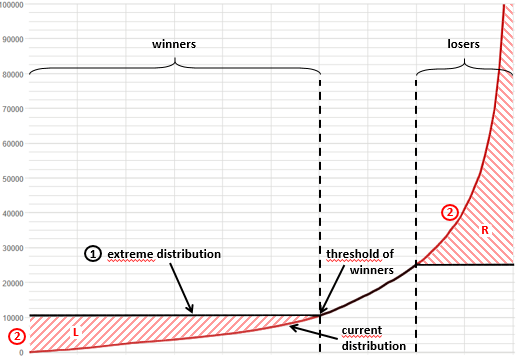
\includegraphics[width=\textwidth]{../figures/questionnaire/algo_1-2.PNG}
  \end{subfigure} 
  \begin{subfigure}{.49\textwidth}
    \caption[]{Steps 3 and 4.}
    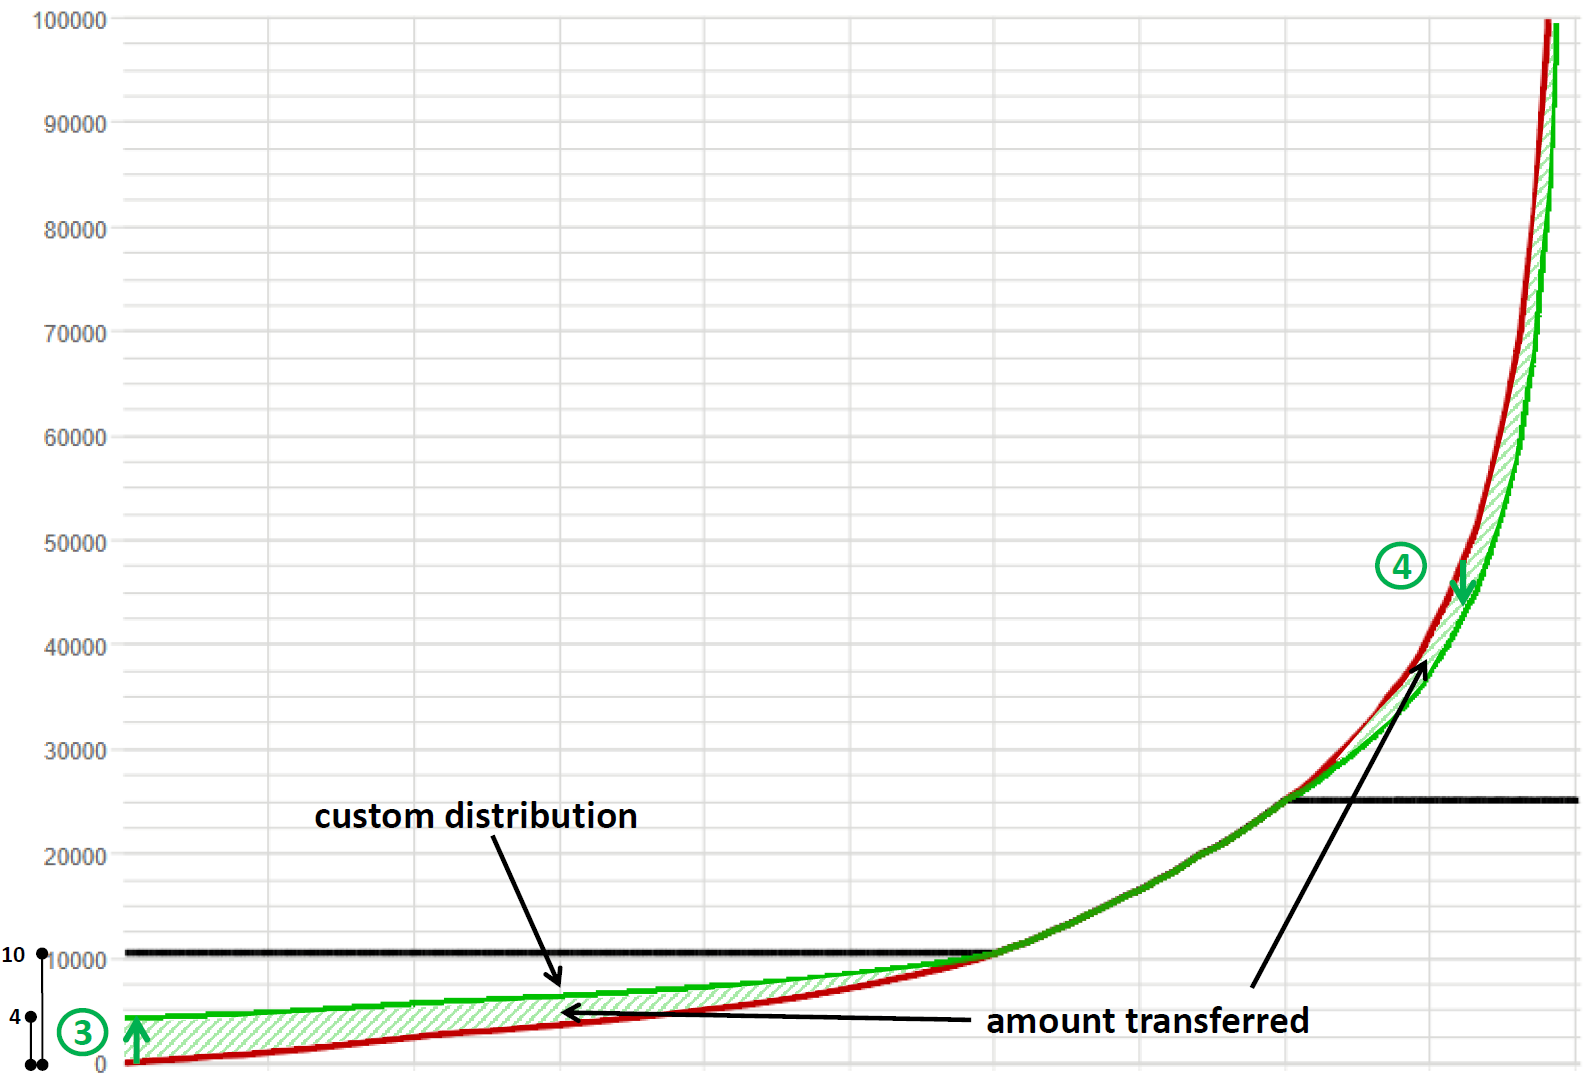
\includegraphics[width=\textwidth]{../figures/questionnaire/algo_3-4_full.PNG}
  \end{subfigure}
\end{figure}

\begin{enumerate}
    \item Define the \textit{extreme distribution} as the current distribution bounded by the income thresholds of winners and losers. In other words, draw two horizontal lines at each end of the distribution, by setting the incomes of winners to the income of the richest winner, and those of losers to the income of the poorest loser.
    \item Compute what can be redistributed on either side as the area between the extreme and current distributions: what can be given to winners on the left side ($L$) or taken on the right side ($R$). If and only if what can be given is lower than what can be taken ($L < R$, as in the above Figure% \ref{fig:algo}
    ), the left side is binding, and it determines the \textit{amount transferred} from the rich to the poor: $\min\{L;\,R\} \cdot degree$.
    \item On the binding side, define the custom distribution as a linear mixture between the current and extreme distributions, with the mixture parameter set by the \textit{degree of redistribution}. In other words, starting from the current distribution, narrow the gap with the extreme distribution by a factor \textit{degree}.
    \item Adjust the non-binding side by narrowing the gap with the extreme distribution, using the unique mixture parameter that preserves aggregate income (so that the amount transferred is the same on both sides).\footnote{While we do not account for behavioral responses, one can adjust the algorithm to account for them. It suffices to define a post-reform aggregate income, which can be lower than the pre-reform one if the reform disincentivizes economic activity.}
    \item ~[Optional step, used in the survey.] To increase the demogrant (i.e. the lowest income) and make the reform more progressive on the left side, try to replace the left side with a straight line. In other words, find the demogrant and the straight line between the demogrant and the threshold of winners that respects the amount transferred. If this straight line crosses the current distribution or if it implies a regressive redistribution (in that some incomes would increase less than higher incomes), abandon the straight line and keep the custom redistribution as is.
\end{enumerate}

% \clearpage
% \renewcommand{\url}[1]{\href{#1}{Link}}
% \putbib
% \end{bibunit}